
\documentclass[
  fontsize=10pt, % Base font size
  twoside=true, % Use different layouts for even and odd pages (in particular, if twoside=true, the margin column will be always on the outside)
  % open=any, % If twoside=true, uncomment this to force new chapters to start on any page, not only on right (odd) pages
  secnumdepth=1, % How deep to number headings. Defaults to 1 (sections)
  %chapterprefix=true, % Uncomment to use the word "Chapter" before chapter numbers everywhere they appear
  %chapterentrydots=true, % Uncomment to output dots from the chapter name to the page number in the table of contents
  numbers=noenddot, % Comment to output dots after chapter numbers; the most common values for this option are: enddot, noenddot and auto (see the KOMAScript documentation for an in-depth explanation)
  % draft=true, % If uncommented, rulers will be added in the header and footer
  % overfullrule=true, % If uncommented, overly long lines will be marked by a black box; useful for correcting spacing problems
]{kaobook}

% Choose the language
\usepackage[english]{babel} % Load characters and hyphenation
\usepackage[english=british]{csquotes}  % English quotes
\usepackage{tablefootnote}

% Load packages for testing
\usepackage{blindtext}
%\usepackage{showframe} % Uncomment to show boxes around the text area, margin, header and footer
%\usepackage{showlabels} % Uncomment to output the content of \label commands to the document where they are used

% Load the bibliography package
% \usepackage{styles/kaobiblio}
% \addbibresource{book-template.bib} % Bibliography file

% Load the package for hyperreferences
\usepackage{styles/kaorefs}

% Load mathematical packages for theorems and related environments. NOTE: choose only one between 'mdftheorems' and 'plaintheorems'.
\usepackage{styles/mdftheorems}
%\usepackage{styles/plaintheorems}

% \graphicspath{{images/}{./}} % Paths in which to look for images

\makeindex[columns=3, title=Alphabetical Index, intoc] % Make LaTeX produce the files required to compile the index

\makeglossaries % Make LaTeX produce the files required to compile the glossary

\makenomenclature % Make LaTeX produce the files required to compile the nomenclature



%----------------------------------------
% HL
%----------------------------------------

% \usepackage[backend=biber,natbib=true,maxcitenames=2,maxbibnames=10,giveninits=true,isbn=false,doi=false,url=false,defernumbers=true,style=numeric,sorting=ydnt]{biblatex} 
\usepackage[backend=bibtex,natbib=true,style=authoryear,citestyle=authoryear,maxcitenames=2,maxbibnames=10,giveninits=true,isbn=false,doi=false,dashed=false]{biblatex}
\bibliography{refs/3db} % Bibliography file
%-- remove the In:
\renewbibmacro{in:}{}
%-- remove the "" before/after the title of the paper
\DeclareFieldFormat[article, inbook, incollection, inproceedings, misc, thesis, unpublished]{title}{#1}



% Command to print a citation in the margins
\newcommand{\sidecitet}[1]{% The optional parameter is the 
%vertical shift; 
%the mandatory one is the citation key
  \citet{#1}% With this we print the marker in the text and add the item to the 
  %bibliography at the end \margincitation
  \marginnote{\citeauthor*{#1} (\citeyear{#1}), \citetitle{#1}\\}% 
  %Create a marginnote for each item
}

\newcommand{\sidecitep}[1]{% The optional parameter is the 
%vertical shift; 
%the mandatory one is the citation key
  \citep{#1}% With this we print the marker in the text and add the item to the 
  %bibliography at the end \margincitation
  \marginnote{\citeauthor*{#1} (\citeyear{#1}), \citetitle{#1}\\}% 
  %Create a marginnote for each item
}

\renewcommand{\ie}{ie}
\renewcommand{\eg}{eg}
% \newcommand{\reffig}[1]{Figure~\ref{#1}}
% \newcommand{\refsec}[1]{Section~\ref{#1}}
\newcommand{\refchap}[1]{Chapter~\ref{#1}}

\setcounter{margintocdepth}{1}
\setcounter{tocdepth}{1}

\usepackage{subcaption}
\usepackage{fontawesome}
\usepackage{boxedminipage}
\usepackage{gensymb}
\usepackage{listings}
\usepackage{color}
\definecolor{codegreen}{rgb}{0,0.6,0}
\definecolor{codegray}{rgb}{0.5,0.5,0.5}
\definecolor{codepurple}{rgb}{0.58,0,0.82}
\definecolor{backcolour}{rgb}{0.95,0.95,0.92}
\lstdefinestyle{mystyle}{
    backgroundcolor=\color{backcolour},   
    commentstyle=\color{codegreen},
    keywordstyle=\color{magenta},
    numberstyle=\tiny\color{codegray},
    stringstyle=\color{codepurple},
    basicstyle=\footnotesize,
    breakatwhitespace=false,         
    breaklines=true,                 
    captionpos=b,                    
    keepspaces=true,                 
    numbers=left,                    
    numbersep=5pt,                  
    showspaces=false,                
    showstringspaces=false,
    showtabs=false,                  
    tabsize=2
}
\lstset{style=mystyle,basicstyle=\ttfamily\footnotesize,breaklines=true}
\usepackage{xurl}
\usepackage{hyperref}
\hypersetup{breaklinks=true}

\setcounter{secnumdepth}{3}


%----------------------------------------------------------------------------------------

\begin{document}

%----------------------------------------------------------------------------------------
% BOOK INFORMATION
%----------------------------------------------------------------------------------------


\title{3D modelling of the built environment}
\author{Ken Arroyo Ohori \hspace{7mm} Hugo Ledoux \hspace{7mm} Ravi Peters}
\date{\texttt{v0.1}}

% \publishers{\includegraphics[width=\linewidth]{front-back/saba.png}}

%----------------------------------------------------------------------------------------

% \frontmatter % Denotes the start of the pre-document content, uses roman numerals

%----------------------------------------------------------------------------------------
% OPENING PAGE
%----------------------------------------------------------------------------------------

%\makeatletter
%\extratitle{
% % In the title page, the title is vspaced by 9.5\baselineskip
% \vspace*{9\baselineskip}
% \vspace*{\parskip}
% \begin{center}
%   % In the title page, \huge is set after the komafont for title
%   \usekomafont{title}\huge\@title
% \end{center}
%}
%\makeatother

%----------------------------------------------------------------------------------------
% COPYRIGHT PAGE
%----------------------------------------------------------------------------------------

% %!TEX root = ../3dbook.tex


\makeatletter
% \uppertitleback{\@titlehead} % Header

\lowertitleback{
  
\textcopyright\ 2020--2022 \, Ken Arroyo Ohori, Hugo Ledoux, and Ravi Peters

\medskip

\ccLogo\ \ccAttribution\ This work is available under a Creative Commons Attribution 4.0 International License.
For license details, see \url{http://creativecommons.org/licenses/by/4.0/}

\medskip

v0.8 --- 2022-02-04 --- Initial release (for 2021--2022 Q3 course)

\medskip
\medskip

\textbf{Download latest version} \\
The latest version of this book can be downloaded in PDF at\\ 
\url{https://github.com/tudelft3d/3dbook/releases}

\medskip

\textbf{Source code} \\
The source code, in \LaTeX, is openly available at\\
\url{https://github.com/tudelft3d/3dbook}

\medskip

\textbf{Errors? Feedback?} \\
Please report errors at\\
\url{https://github.com/tudelft3d/3dbook/issues}

\medskip

\textbf{Colophon} \\
This book was typeset with \LaTeX\ using the \texttt{kaobook} class (\url{https://github.com/fmarotta/kaobook}).
% \mbox{{\fanciestfont{}Feijoa}}, \texttt{GT Pressura} and $\mathrm{Asana\ Math}$ typefaces.
% The figures were created using Ipe, OmniGraffle, Affinity Designer, or Blender.
% The cover image is the SRTM dataset around the Caribbean island Saba, which at 887m is the highest point of the entire Kingdom of the Netherlands; it was rendered with the R package \emph{rayshader}.
 

}
\makeatother







%----------------------------------------------------------------------------------------
% OUTPUT TITLE PAGE AND PREVIOUS
%----------------------------------------------------------------------------------------

% Note that \maketitle outputs the pages before here

% If twoside=false, \uppertitleback and \lowertitleback are not printed
% To overcome this issue, we set twoside=semi just before printing the title pages, and set it back to false just after the title pages
% \KOMAoptions{twoside=semi}
% \maketitle
% \KOMAoptions{twoside=false}

%----------------------------------------------------------------------------------------
% PREFACE
%----------------------------------------------------------------------------------------

% %!TEX root = ../3dbook.tex

% About this book
% from a course, bundle of lecture notes
% link to videos
% acknowledgements


\chapter*{Preface}

This book is the bundle of lecture notes written for the course \emph{3D modelling of the built environment} (GEO1004), which is part of the MSc in Geomatics at the Delft University of Technology.
Each chapter corresponds to a lesson of the course, and each lesson is accompanied by a short video introducing the key ideas and/or explaining some parts of the lessons.
This book, the videos and other materials are freely available online on the website of the course:

\url{https://3d.bk.tudelft.nl/courses/geo1004/}

\paragraph*{Contents}
The book describes the main ways in which the built environment is modelled in three dimensions, covering material from low-level data structures for generic 3D data to high-level semantic data models for cities.

\paragraph*{Who is this book for?}
The book is written for students in Geomatics at the MSc level, but we believe it can be also used at the BSc level.
The main prerequisites are GIS and programming.

\paragraph*{Acknowledgements.}
We would like to thank Francesca Noardo, who contributed significant parts of the BIM chapter.
Also thank you to all the students who helped us by pointing out errors and typos, especially Zhaiyu Chen and Bingshiuan Tsai.






%----------------------------------------------------------------------------------------
% TABLE OF CONTENTS & LIST OF FIGURES/TABLES
%----------------------------------------------------------------------------------------

\begingroup % Local scope for the following commands

% Define the style for the TOC, LOF, and LOT
%\setstretch{1} % Uncomment to modify line spacing in the ToC
%\hypersetup{linkcolor=blue} % Uncomment to set the colour of links in the ToC
\setlength{\textheight}{23cm} % Manually adjust the height of the ToC pages

% Turn on compatibility mode for the etoc package
\etocstandarddisplaystyle % "toc display" as if etoc was not loaded
\etocstandardlines % "toc lines as if etoc was not loaded

% \tableofcontents % Output the table of contents

% \listoffigures % Output the list of figures

% Comment both of the following lines to have the LOF and the LOT on different pages
% \let\cleardoublepage\bigskip
% \let\clearpage\bigskip

% \listoftables % Output the list of tables

\endgroup

%----------------------------------------------------------------------------------------
% MAIN BODY
%----------------------------------------------------------------------------------------

% \mainmatter 
\setchapterstyle{kao} % Choose the default chapter heading style

\setlength{\overflowingheadlen}{\linewidth}
\addtolength{\overflowingheadlen}{\marginparsep}
\addtolength{\overflowingheadlen}{\marginparwidth}
\renewpagestyle{scrheadings}{%
  {\hspace{-\marginparwidth}\hspace{-\marginparsep}\makebox[\overflowingheadlen][l]{%
    \parbox[t][1.7cm][c]{2em}{\hfill\thepage}%
    \makebox[2em][c]{\rule[-1.03cm]{1pt}{1.55cm}}%
    \parbox[t][1.7cm][c]{\textwidth}{\leftmark}}}%
  {\makebox[\overflowingheadlen][r]{%
    \parbox[t][1.7cm][c]{\textwidth}{\hfill\rightmark}%
    \makebox[2em][c]{\rule[-1.03cm]{1pt}{1.55cm}}%
    \parbox[t][1.7cm][c]{2em}{\thepage}}}%
  {\makebox[\overflowingheadlen][r]{%
    \parbox[t][1.7cm][c]{\textwidth}{\hfill\rightmark}%
    \makebox[2em][c]{\rule[-1.03cm]{1pt}{1.55cm}}%
    \parbox[t][1.7cm][c]{2em}{\thepage}}}%
}{%
  {}%
  {}%
  {}%
}
\renewpagestyle{plain.scrheadings}{
  {}%
  {}%
  {}
}{
  {\thepage}%
  {\parbox[t][0cm][c]{\overflowingheadlen}{\ccbysa\ Ken Arroyo Ohori, Hugo Ledoux, Ravi Peters and Francesca Noardo. This work is licensed under a Creative Commons Attribution 4.0 International License (\url{http://creativecommons.org/licenses/by/4.0/})\newline(last update: \today)}}%
  {}
}
\pagestyle{scrheadings}
\newcommand*{\thelesson}{?.?}

% %!TEX root = ../3dbook.tex

\setchapterpreamble[u]{\margintoc}

\graphicspath{{dmds/}}
% \renewcommand*{\thelesson}{1.1}

\chapter{Introduction to 3D modelling of the built environment: reality, data models and data structures}%
\label{chap:dmds}

% 3D modelling and representations

The 3D modelling of the built environment involves the creation, manipulation and use of 3D digital representations of real-world objects, including buildings, terrains and infrastructure.
Over the years, a variety of such representations have been created, each of them modelling objects in a different way and targetting different applications.

% What can be stored and what should be stored

These representations usually include a mix of \emph{geometric} (\ie\ description of shape)\marginnote{geometry}\index{geometry}, \emph{topological}\marginnote{topology}\index{topology} (\ie\ adjacencies and connectivity) and \emph{semantic}\marginnote{semantics}\index{semantics} (\ie\ attributes and other properties) information.
While these can all be combined in arbitrary ways, in practice it is desirable to limit the complexity modelling only the aspects that are needed for an application, and to do so in a manner that is both flexible (to be applicable to all the different objects that can be modelled) and consistently structured (to allow for automated processing using simple rules).

% Compromises

All of these desirable characteristics oppose each other, and so solutions involve finding the compromises that suit a particular application best.
However, since different applications tend to have some elements in common, it is not necessary to build a completely new representation for each application.
Instead, we can reuse representational aspects as a sort of building blocks, from which we can then come up with a good solution for a use case we are working on.

% Contents

In this introductory lesson to the course, we start by explaining how this process is split into a hierarchy working at different levels (from high to low).
While the exact definition of these levels is a bit arbitrary, we follow a common model for geographic information, splitting them into spatial concepts, data models and data structures.
We introduce each of these levels in its own section, including some basic examples for each.
Throughout most of the course, we will look at different data models and data structures in detail.

\section{Hierarchical abstractions in the 3D modelling process}

3D modelling is done through a series of abstractions of the real world, each working at a different abstraction level.
For instance, a typical high-level abstraction could divide the world into discrete objects (\eg\ individual buildings or plots of land), whereas a lower-level abstraction could divide each surface of a wall into triangles (\ie\ meshing) while satisfying certain characteristics (\eg\ minimum angles).
Each abstraction is thus an engineered partial solution to a complex modelling problem, which comes with its own technical choices, advantages and disadvantages, and applications for which it is suitable (or not).

For example, a 3D city model can be stored in a \texttt{.json} file where its entities are structured according to the CityJSON data model, with geometries represented as solids, and where each semantic surface is a triangulated mesh.
Alternatively, we can have a classified point cloud of the same city stored in an indexed series of \texttt{.las} files representing tiles.
Out of these two representations, the point cloud can be easily used as base elevation data or for many visualisation-based operations with comparatively little processing, but even simple spatial analysis operations (\eg\ counting the number of buildings or computing their volume) can be very complex.
On the other hand, the 3D city model could be used for complex spatial analysis operations (\eg\ wind and solar radiance simulations; Figure~\ref{fig:applications}), but some objects that are present in the real-world (\eg\ trees and fences) might be lost in the model or present only as artefacts.

\begin{figure}
\centering
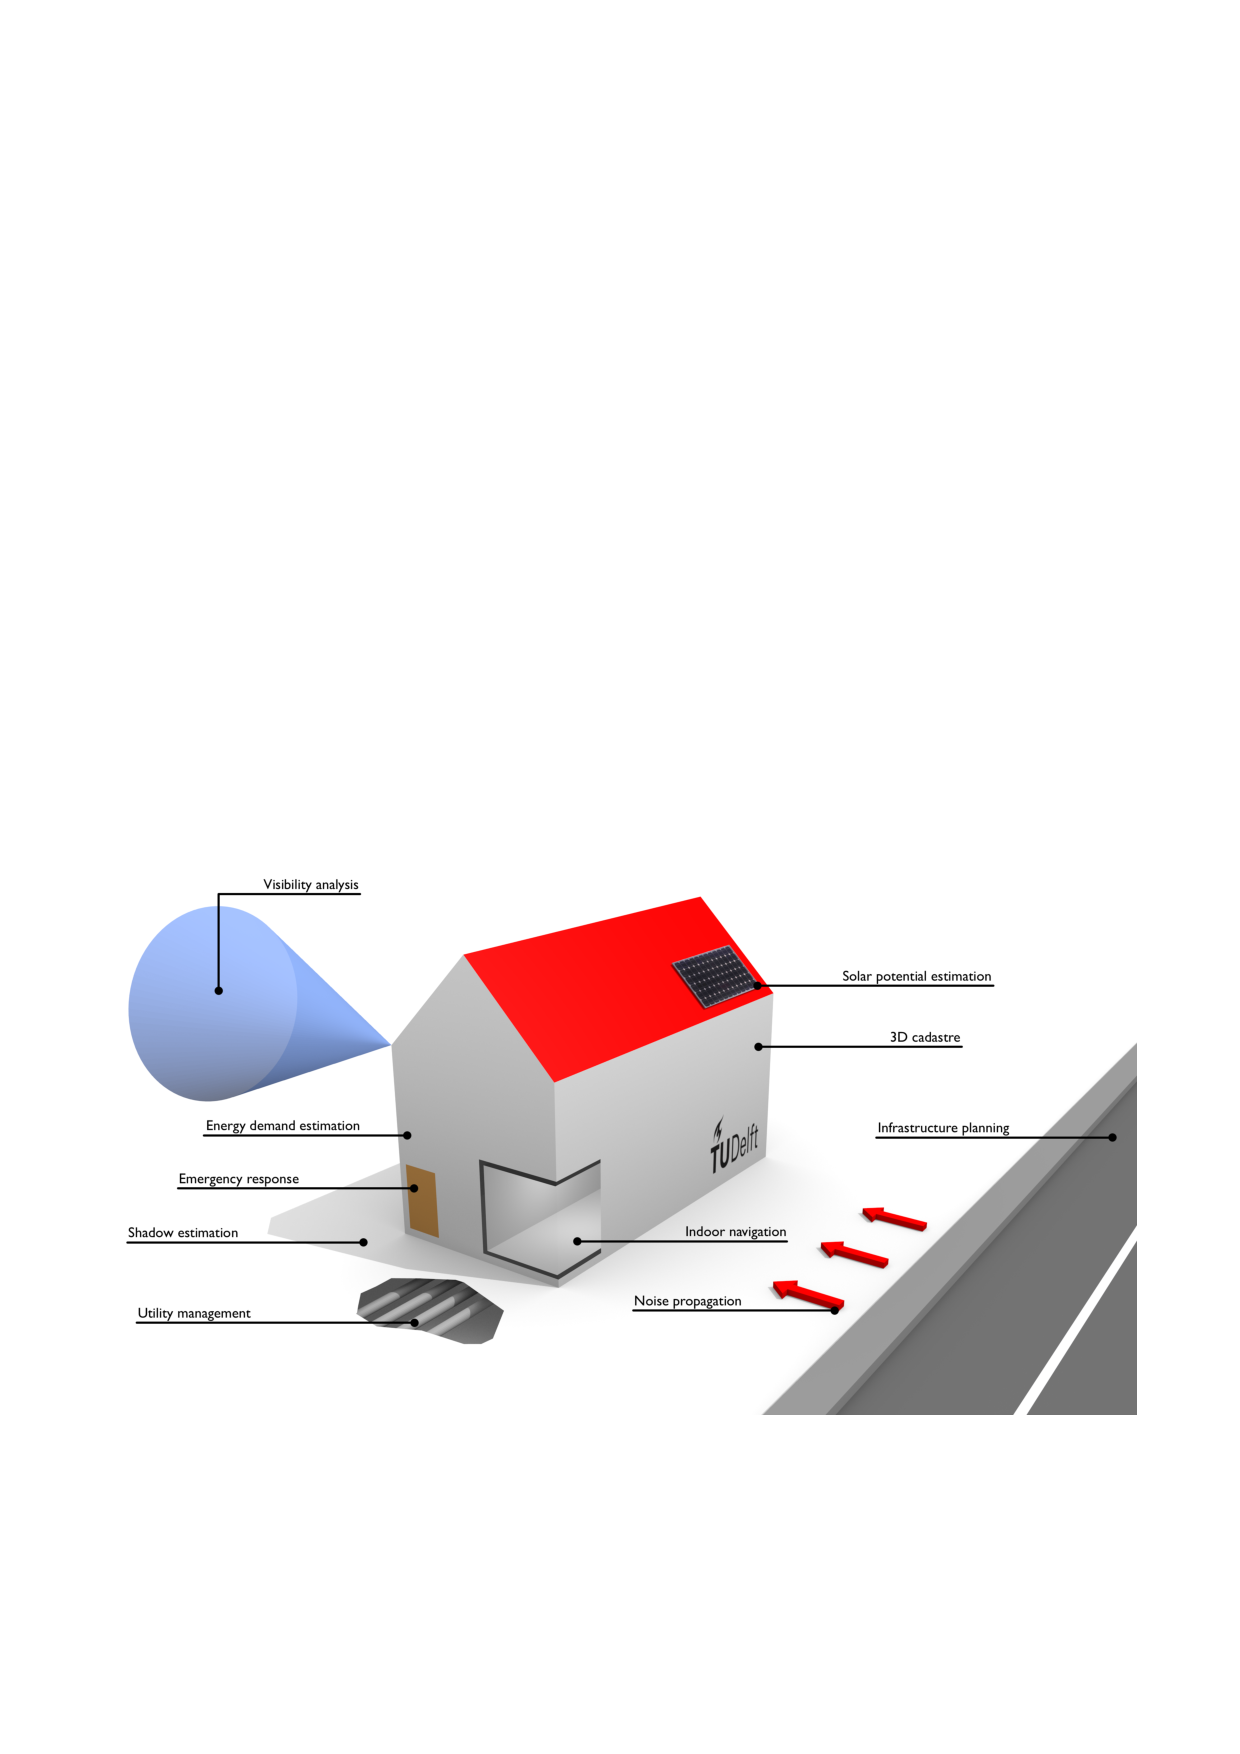
\includegraphics[width=\linewidth]{figs/applications.pdf}
\caption{Some typical applications of 3D city models~\citep{Biljecki15a}.}%
\label{fig:applications}
\end{figure}

In the next sections, we look at three different levels at which abstractions are made: (i) spatial concepts, which work entirely on the basis of human-level congnition; (ii) data models, which are higher-level abstractions closer to the way we structure the world; (iii) and data structures, which are lower-level abstractions close to how they are implemented in a computer.

Even if it is not entirely clear at this point, this means that there can be many possible data models that use a certain spatial concept, and that there can be many different data structures that encode the same data model, each of which is best suited for a given application.

\section{Spatial concepts}

In order to conceptualise and structure the real world, 3D models of the built environment rely on some common spatial concepts.
Some of the most common ones are:

\begin{description}

\item[Geoinformation processing (\ie\ the geoinformation chain)]
From\marginnote{geoinformation chain}\index{geoinformation chain} a practical perspective, a common way to consider how space is structured is based on the usual steps in the geoinformation chain (or pipeline).
This considers that one starts from the acquisition of data, either through traditional measurements (using anything from a tape measure to a total station) or using a variety of sensing technologies, including active methods using the reflections of electromagnetic waves (\eg\ all forms of lidar and radar) and vibrations (\eg\ underwater echo sounding and seismic methods), as well as passive methods (\eg\ digital images using any spectrum).

These `raw' measurements are then used to create simple primitives (\eg\ the points in a point cloud or the plane equation of a wall), and these are then further processed and assembled to create more complex 3D objects.

For instance, a typical process can go from a set of lidar full waveforms to a point cloud by deciding on appropriate return power thresholds, then to a series of meshes by reconstructing surfaces and fitting planes, and finally to a 3D city model with semantic surfaces by classifying and assembling the surfaces into 3D objects.
In every step of such a process, there is certain amount of information loss, but (ideally) the information that remains is more structured and meaningful.

\item[Objects and fields]
From a theoretical GIS standpoint, the typical way to conceptualise space recognises two ways of looking at the world: \emph{objects} and \emph{fields}.
The objects\marginnote{object}\index{object} view considers that space is empty and is populated by discrete objects.
In many cases, this results in an approach where objects are modelled individually (\eg\ a building modelled as a set of surfaces), although they can also be aggregated or generalised into (\eg\ a set of adjacent buildings with the same height modelled as a single block).

By contrast, the fields\marginnote{field}\index{field} view considers that there are certain attributes that fill space and have a value everywhere in it.
The typical examples are physical characteristics, such as the elevation of a terrain, the temperature or the wind speed.
Since we generally cannot know or store the values of fields in every possible location, of which there might be infinitely many, the standard approach is to mathematically model an approximation (\eg\ elevation modelled as an interpolated set of points).

% \item[Geometry, topology and semantics]

\item[Euclidean, Cartesian and point set geometry]
When we model objects mathematically, we often rely on abstract geometric shapes, such as point, lines and planes.
The simplest mathematical descriptions for these are based on \emph{Euclidean geometry}\marginnote{Euclidean geometry}\index{Euclidean geometry}.
Euclidean geometry starts from a small set of geometric axioms considered to be intuitively obvious (Figure~\ref{fig:line}).
Using these axioms, it is possible to construct more complex objects (\eg\ a triangle covering the area between three points) and to define properties, such as relative distances, angles and areas.
However, objects in Euclidean geometry do not have an absolute position in space.

\begin{marginfigure}
\centering
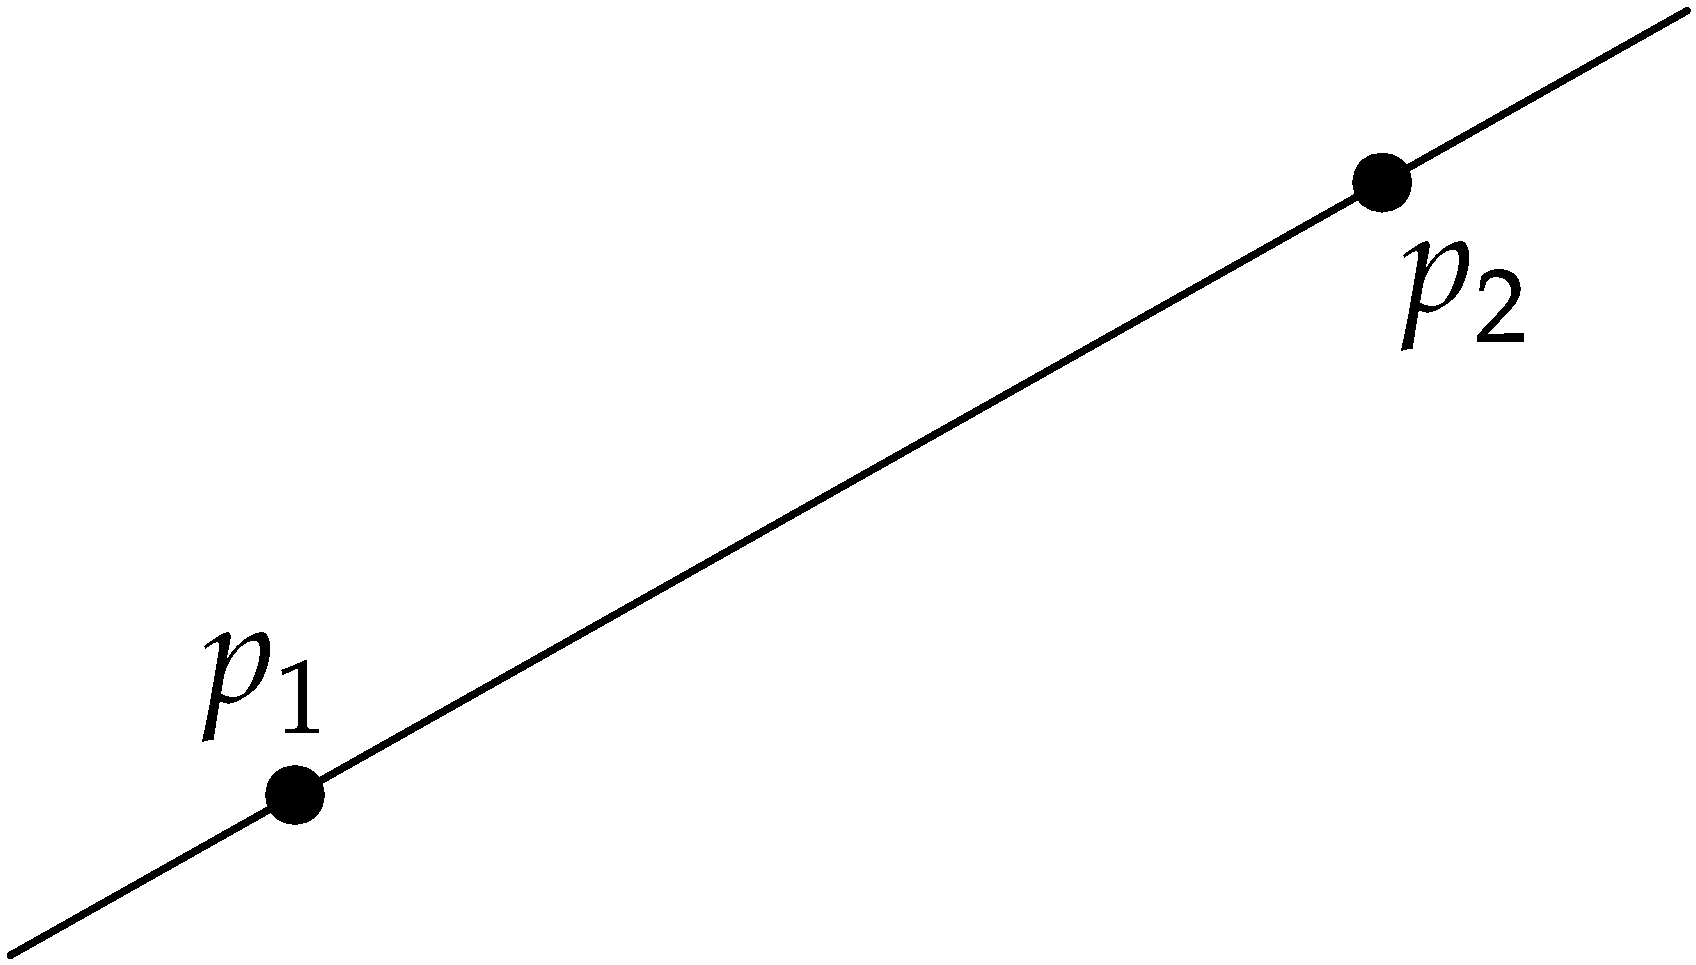
\includegraphics[width=\linewidth]{figs/line.pdf}
\caption{Since there is exactly one line that passes through any pair of points, two points can be used to describe a line in Euclidean geometry.}%
\label{fig:line}
\end{marginfigure}

Where this notion is required, analytic or \emph{Cartesian geometry}\marginnote{Cartesian geometry}\index{Cartesian geometry} adds the concept of coordinates to the objects of Euclidean geometry, which makes it possible to uniquely describe the absolute location of a point (Figure~\ref{fig:point}), the length of a line or the angle between two lines.
This analytic description also makes it possible using algebra to compute the exact value of some properties, such as the distance between two points (as described by their coordinates).

\begin{marginfigure}
\centering
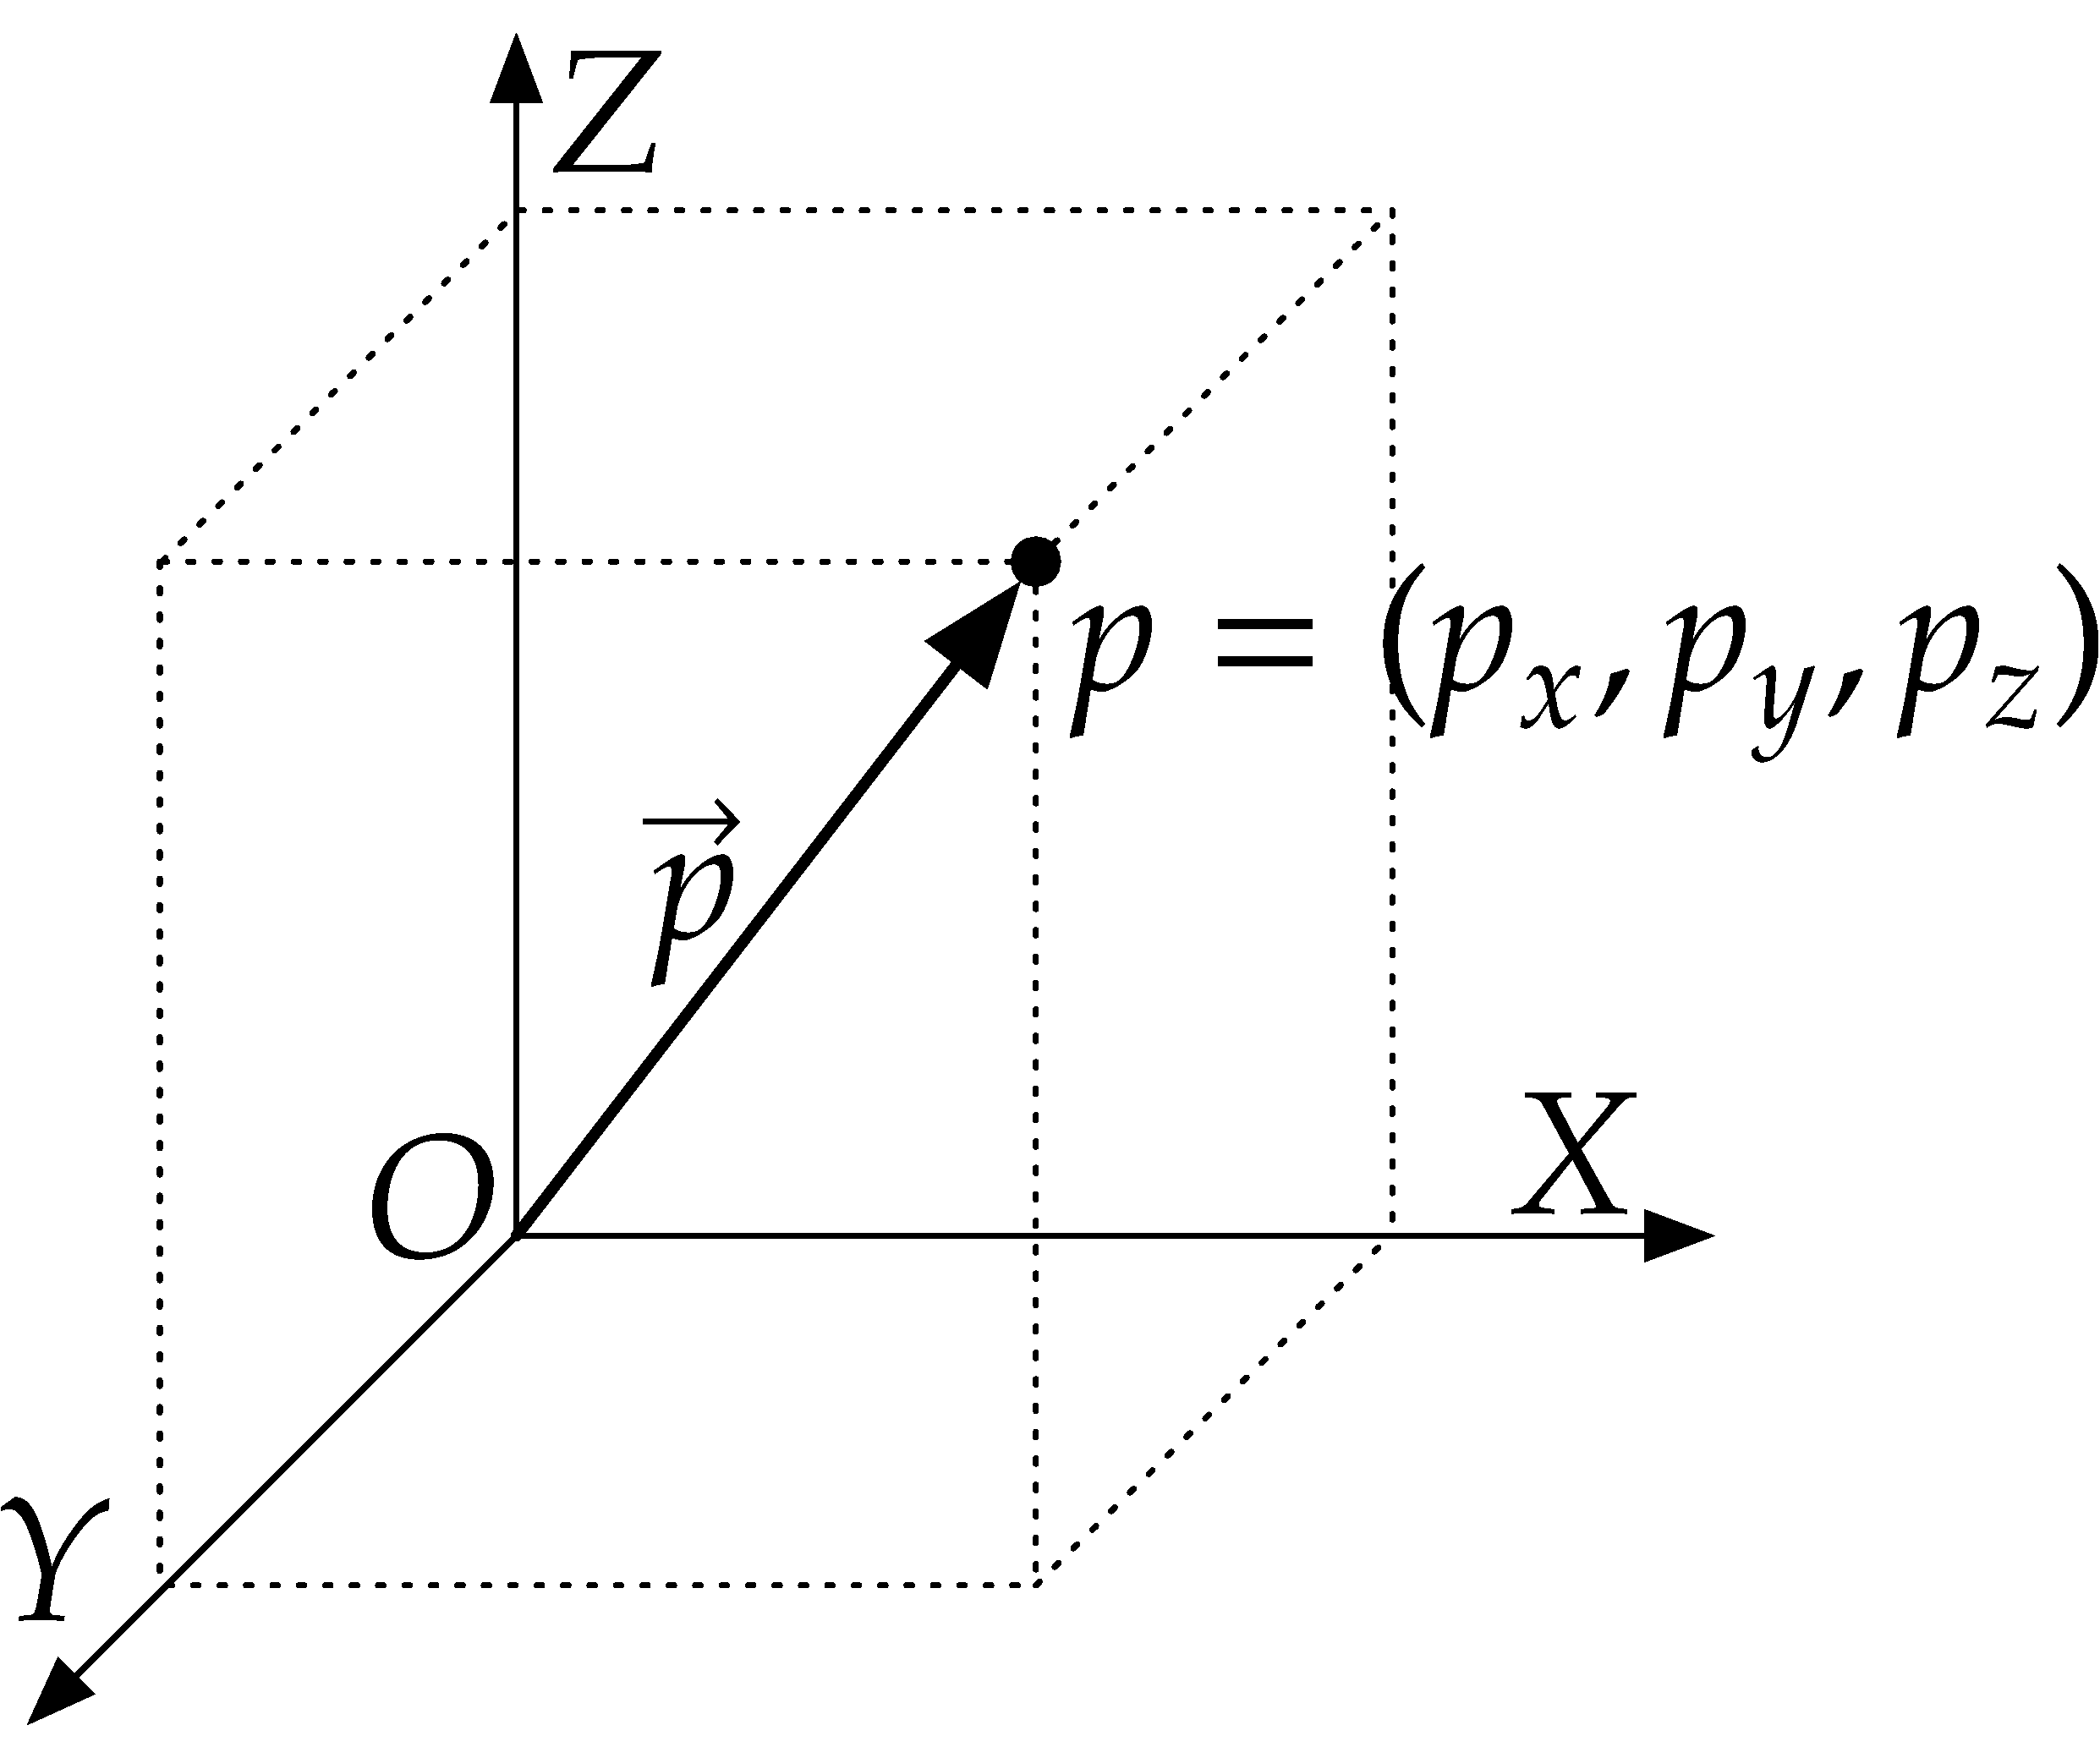
\includegraphics[width=\linewidth]{figs/point.pdf}
\caption{A point in 3D described by an ordered list of three coordinates $(p_x,p_y,p_z)$.}%
\label{fig:point}
\end{marginfigure}

Pure analytical solutions can be however tricky (\eg\ points placed at irrational values), so some other definitions used for modelling objects rely on \emph{point set geometry}\marginnote{point set geometry}\index{point set geometry}.
This method uses the mathematical definitions of sets and of operations between sets to define objects as sets of (often infinitely many) points.
For instance, we can say that a sphere is a point set where the distance to a given point (\ie\ the centre) is equal to a value, or to define an object as the intersection between two other objects (Figure~\ref{fig:boolean}).

\begin{figure}[htbp]
\centering
\begin{subfigure}[b]{0.45\linewidth}
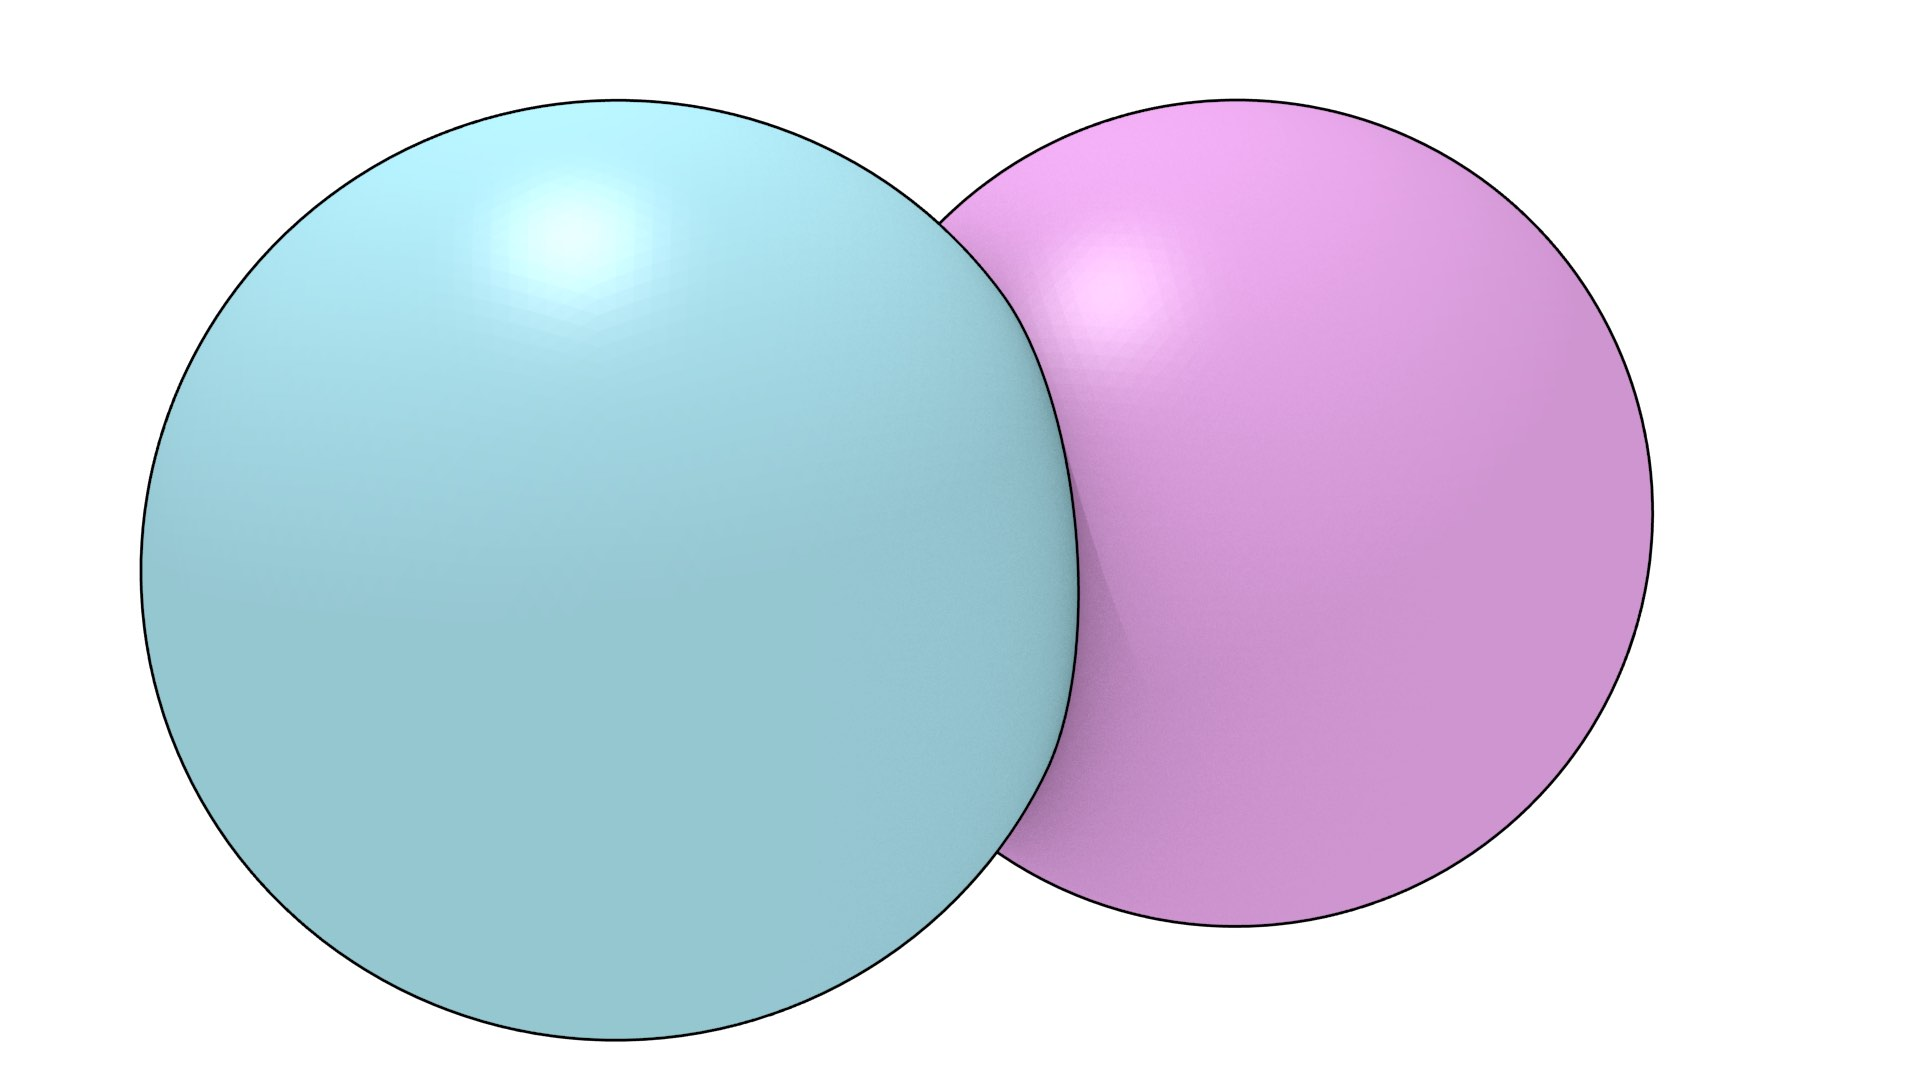
\includegraphics[width=\linewidth]{figs/boolean}
\caption{$\mathbb{A}$ (purple) and $\mathbb{B}$ (blue)}%
\label{subfig:boolean}
\end{subfigure}
\begin{subfigure}[b]{0.45\linewidth}
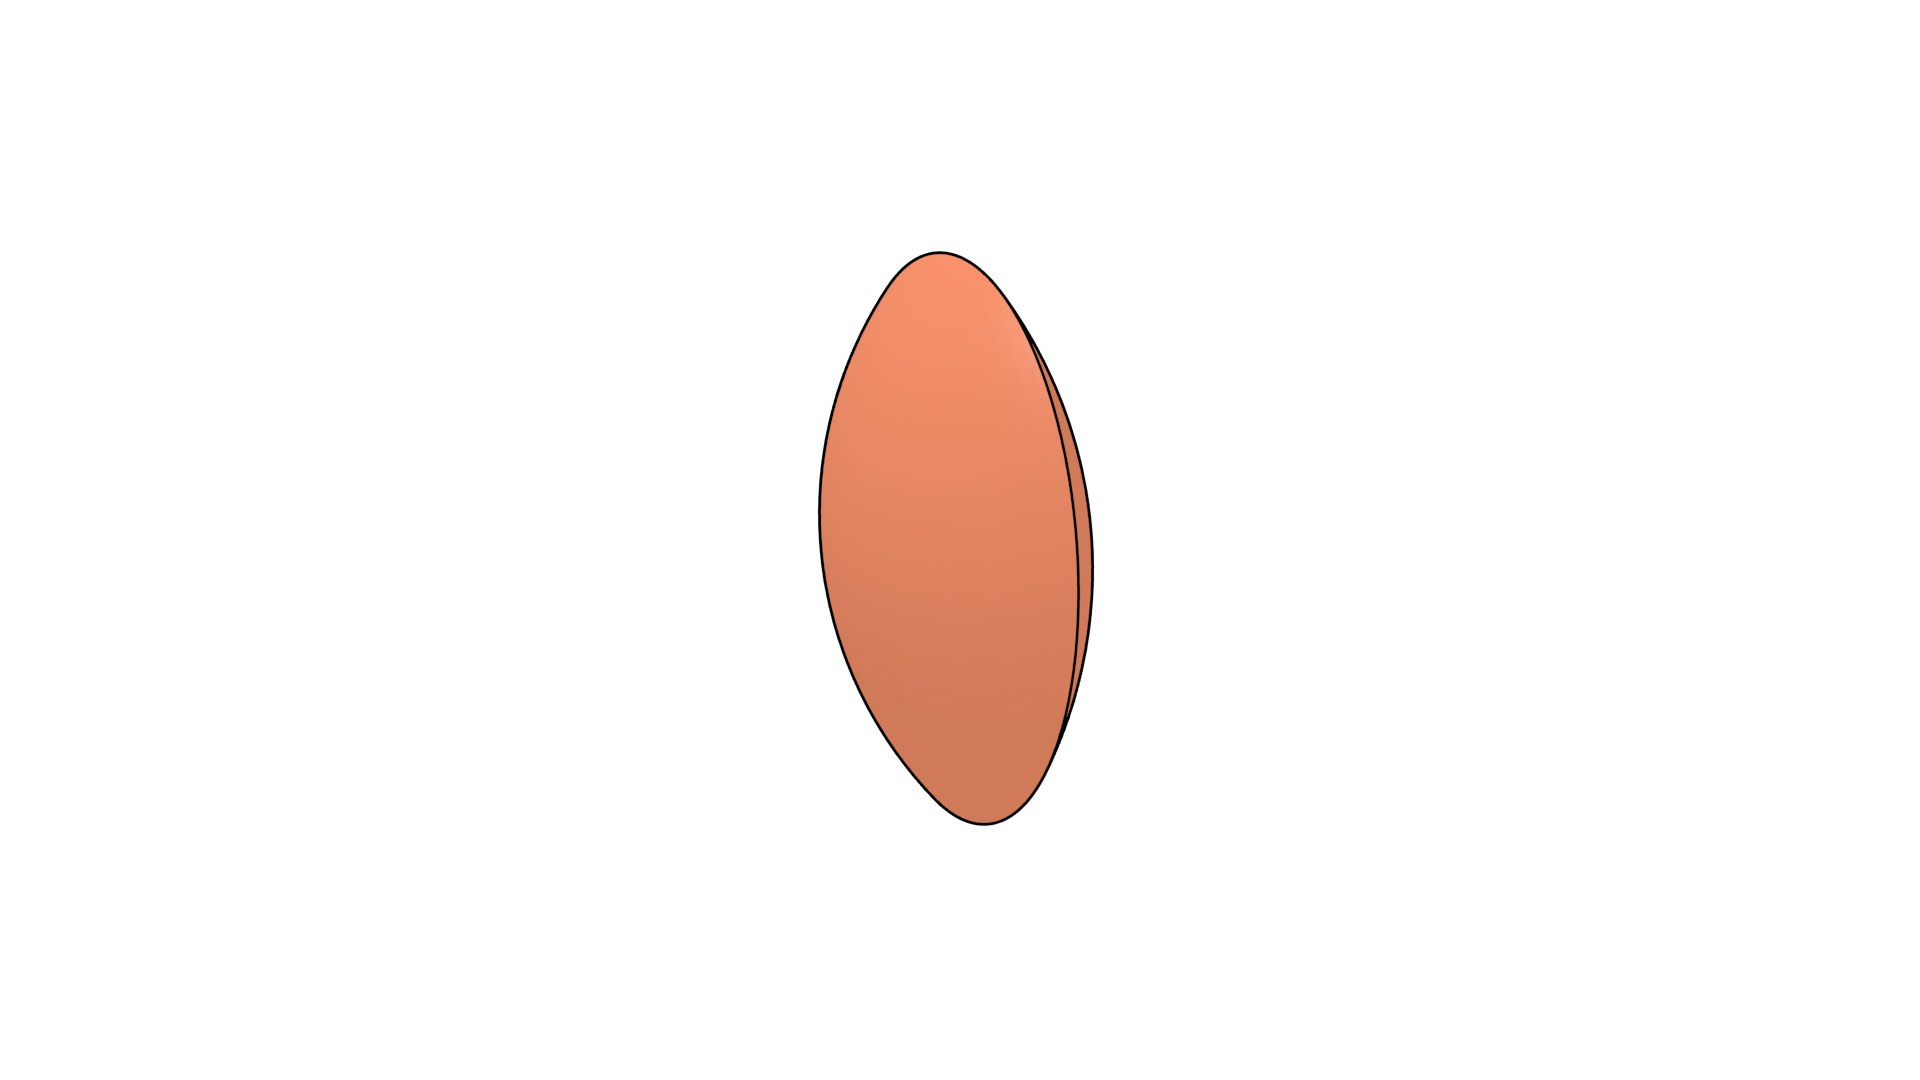
\includegraphics[width=\linewidth]{figs/boolean-intersection}
\caption{Intersection: $\mathbb{A} \cap \mathbb{B}$}%
\label{subfig:boolean-intersection}
\end{subfigure}
\caption{Based on two balls $\mathbb{A}$ and $\mathbb{B}$, other objects that can be defined using Boolean set operations using point set geometry.}%
\label{fig:boolean}
\end{figure}

\item[Graphs and algebraic topology]
The concepts from different branches of geometry are useful to describe the overall shape of objects, but in practice we often need to add concepts of topology as well.
For instance, this is often used to describe relationships between objects, such as adjacency or connectivity.
In the geometric modelling of the built environment, topology is especially important because the standard approach to model complex objects is to divide them into small elements, and thus we also need to describe how these elements are connected.

In its simplest form, topology often takes the form of a \emph{graph}\marginnote{graph}\index{graph}, where the elements are vertices that are connected by (directed) edges.
Vertices often correspond to geometric points and edges to geometric line segments, but this is not always the case.
For instance, in a \emph{dual}\marginnote{duality}\index{duality} representation, vertices can correspond to polygons and the edges connecting them can correspond to the connections between adjacent polygons.

\emph{Algebraic topology}\marginnote{algebraic topology}\index{algebraic topology} takes the concept of a graph further by allowing us to use higher-dimensional objects (\eg\ faces and volumes), which will be used to describe simplices and cells in some of the data models that we will discuss later in the course.
It also makes it possible to describe objects based on sets, as well as to create operations that modify these sets.

% \item[Explicit and implicit geometry]

\end{description}

\section{Data models}

A data model\marginnote{data model}\index{data model} is a high-level formalised way to structure information, generally using a set of abstract classes, relationships between them, and attributes to store information about them.
In the context of geomatics, these classes are often spatial representations of real-world objects.
Some aspects that are typically defined by a data model include the kind of discretisation of space that is used (\eg\ a grid) and the formal mathematical bases of the model (\eg\ describing the basic elements of a data model as tuples).
Certain data models also include formalised operations that can be performed on their defined classes.

Data models are deliberately ambiguous and far from a computer representation, and so implementing them involves various engineering decisions and can be tricky.
Moreover, without some specific encoding rules, different people will make different engineering decisions and thus likely implement a data model very differently.

The typical examples of data models used in (older) geomatics literature are the \emph{raster}\marginnote{raster}\index{raster} and \emph{vector}\marginnote{vector}\index{vector} data models.
These examples are historically accurate because they are clear-cut high-level descriptions that can each be implemented in a variety of ways.
For instance, rasters can be encoded by traversing them in a given order and listing the values in each cell one by one (known as exhaustive enumeration), by splitting it into successive halves of a uniform value using a $k$-d tree, or by compressing it using a Wavelet transform (\eg\ in JPEG 2000 images).

However, it is worth noting that nowadays the term data model is most often used to refer to highly complex abstractions of the real world that are suitable for a particular domain.
These can include a mixture of geometric, topological and semantic components.
Data models are often available in the form of a \emph{schema}\marginnote{schema}\index{schema}---a descriptive document that specifies the data model in a formal manner.
Schemas are often described using UML models (\eg\ CityGML; Figure~\ref{fig:citygml}), although using a computer-processable language (\eg\ JSON schema in CityJSON, EXPRESS in IFC, XSD in CityGML) is generally better since it allows processing the schema, such as for validation.

\begin{figure*}
\centering
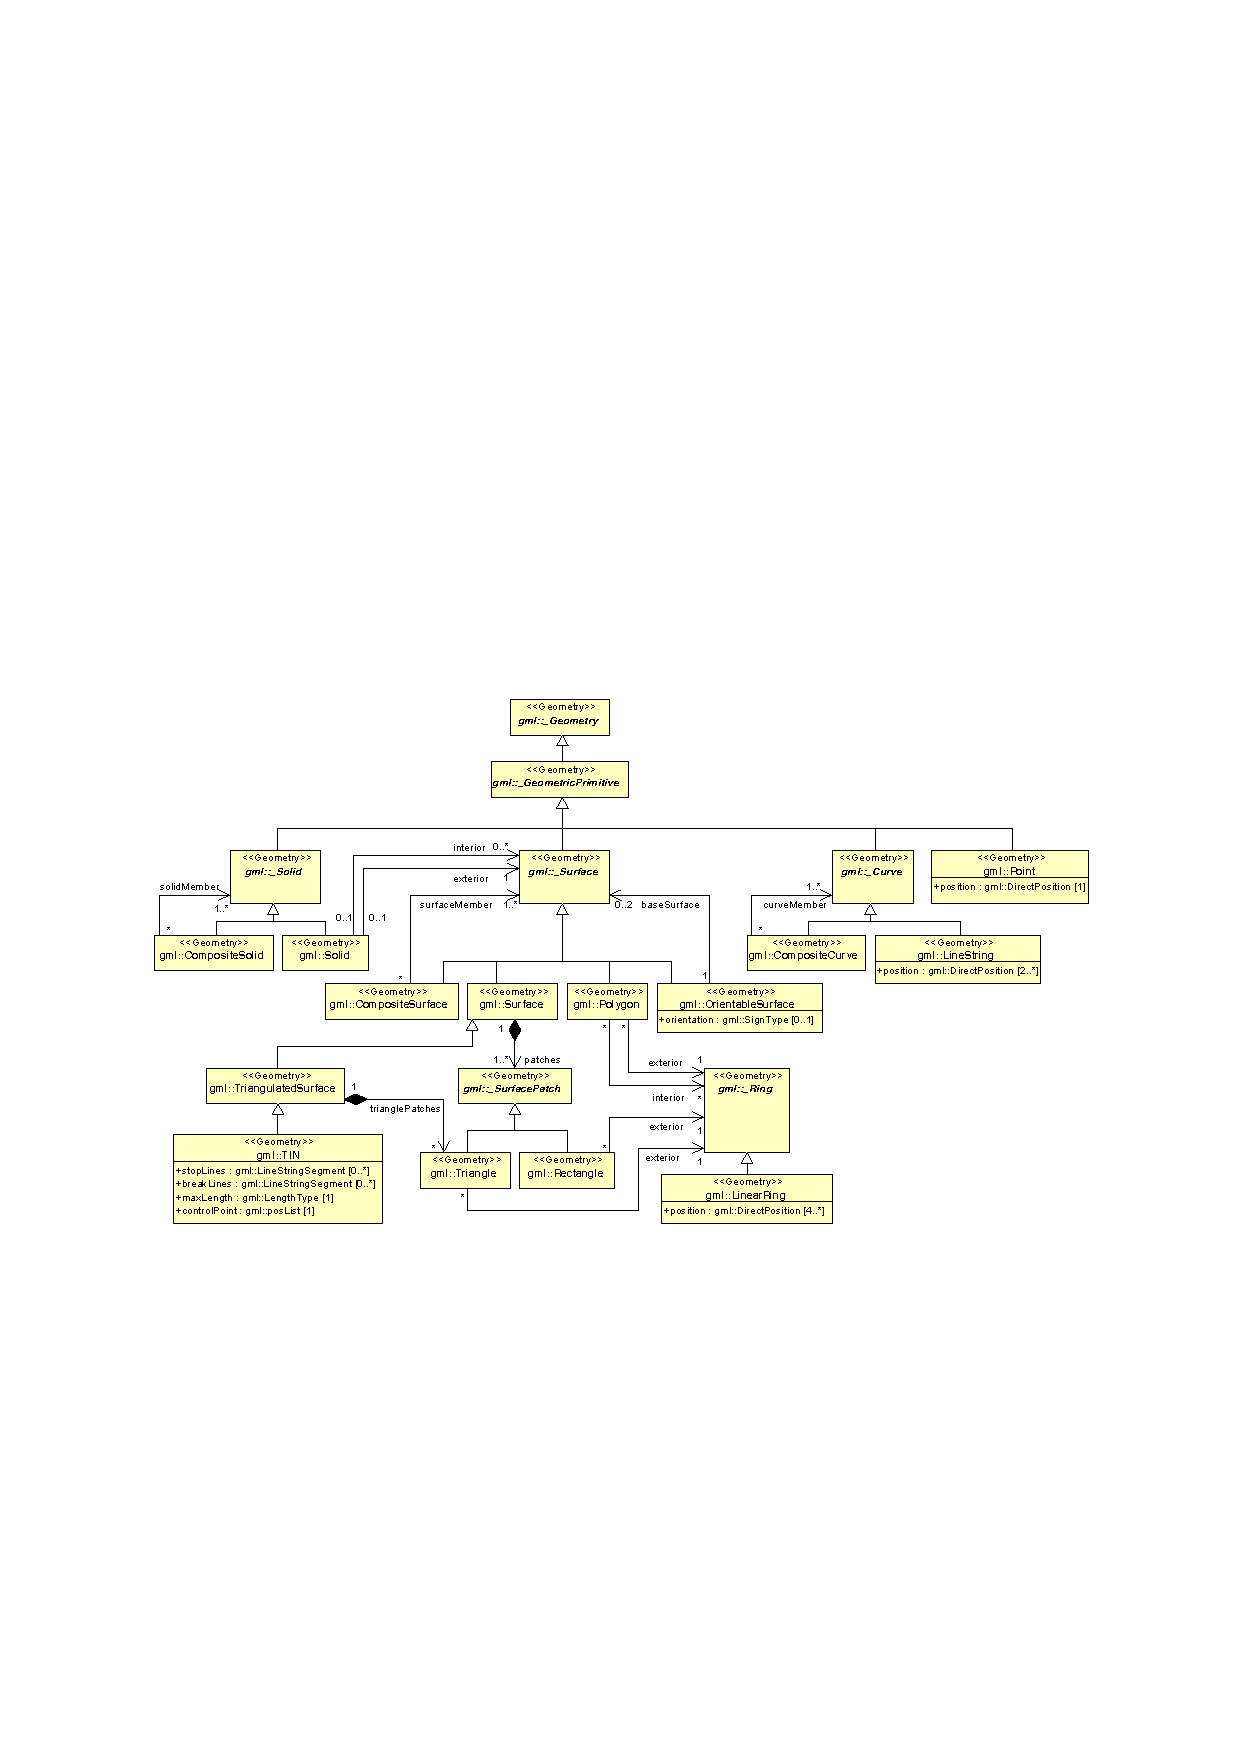
\includegraphics[width=\linewidth]{figs/citygml.pdf}
\caption{The geometry classes used in the CityGML 2.0 standard~\citep{CityGML2.0}.}%
\label{fig:citygml}
\end{figure*}

\section{Data structures}

A data structure\marginnote{data structure}\index{data structure} is a low-level description that specifies how to implement a data model, or occasionally a combination of multiple data models.
Data structures are defined with little to no ambiguity, specifying features such as what sort of storage should be used for a given primitive (\eg\ an array or a linked list). 
As opposed to a data model, creating a computer implementation of a data structure is thus relatively straightforward, and different people implementing the same data structure will end up with very similar implementations.

Data structures can be specified using the same methods as data models, \eg\ UML models, but more explicit descriptions are also possible.
For example, database tuples or table definitions in SQL can be used when a database implementation is expected, or snippets of source code  (generally in the style of the C programming language) can be used when it is expected to be used in memory.

Following a typical example, if we assume that we are implementing a standard vector data model with polygons, we could choose to do so using a half-edge data structure (Figure~\ref{fig:halfedge-2}).
Note that the low-level definition of a half-edge pretty much defines the structure of its computer implementation.

\begin{marginfigure}
\centering
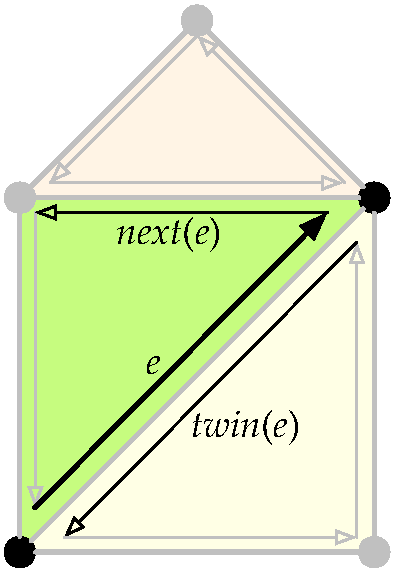
\includegraphics[width=\linewidth]{figs/halfedge-2.pdf}
\caption{The half-edge data structure can store sets of polygons based on elements known as half-edges, which represent an edge within a face.
A half-edge $e$ is related to two vertices (the origin and the destination) and one face, and is linked to its next half-edge (on the same face) and its twin half-edge (on the adjacent face).}%
\label{fig:halfedge-2}
\end{marginfigure}

%%%
%
\section{Exercises}

\begin{enumerate}
	\item What is noisier: the `raw' measurements in the early steps of the geoinformation chain, or the more processed products of the last steps.
	\item Give an example of a field that it not a natural physical characteristic.
	\item Consider whether a point cloud is a data model or a data structure. If it is a data model, what sort of data structure could be used to represent it?
	\item Describe an alternative data structure that can be used to represent the vector data model (\ie\ not the half-edge data structure). What are some advantages/disadvantages of each data structure?
\end{enumerate}



%%%
%
\section{Notes and comments}

\citet{Frank92} is the original source that divides representations into spatial concepts, data models and data structures.
It is partly out of date since it long predates the semantic data models that are used nowadays, but it is still a good paper, and a precursor to the ones we described here.

Chapter 2 of Ken's PhD thesis\footnote{\url{https://3d.bk.tudelft.nl/ken/en/thesis/math.html}} describes all the mathematical notions from this lesson in a bit more detail.
Section 3.1\footnote{\url{https://3d.bk.tudelft.nl/ken/en/thesis/modelling-background.html\#se:spatial-modelling}} lists many data models and data structures with references to the original papers where they came from.

\citet{Couclelis92} is the original source that clearly formalised the difference between objects and fields.
\citet{Goodchild92} links objects and fields to specific computer models that are suitable for them.

\citet{Mantyla88} has an excellent overview of different 3D representations.
Some other good standard alternatives are \citet{Requicha80,Hoffmann92,Foley95}.
A newer book accessible from the campus is \citet{Salomon11}.

 % 1.1
% %!TEX root = ../3dbook.tex

\setchapterpreamble[u]{\margintoc}

\graphicspath{{brep/}}
% \renewcommand*{\thelesson}{1.2}

\chapter{Boundary representation}%
\label{chap:brep}

In the first chapter, we discussed how 3D modelling is done through a series of abstractions of the real world.
One of the chief reasons to do so is to decrease the complexity of what needs to be modelled at each step, with the aim to successively break complex problems into simpler problems until they can be (more easily) solved.

\emph{Boundary representation} works using this principle.
Rather than modelling a 3D object through a volumetric representation, it instead models the object \emph{implicitly} by representing the 2D surface that bounds it (Figure~\ref{fig:cube}).
In this way, it is possible to use one of the many data structures that are used to represent 2D meshes, which are significantly simpler than the data structures used to directly represent arbitrary volumes.

\begin{marginfigure}
\centering
\includegraphics[width=\linewidth]{figs/cube.pdf}
\caption[A cube represented implicitly based on the six square faces that bound it]{A cube can be represented implicitly based on the six square faces that bound it.}%
\label{fig:cube}
\end{marginfigure}

However, it is very important to note that not all 3D objects can be represented using boundary representation with most common 2D mesh data structures without issues.
The main culprits are \emph{non-manifold} objects, which have properties that make representing them ambiguous, as well as objects with holes, which need to be stored using certain techniques.
External data structures might also be needed to keep track of disconnected set of objects, since it might not be possible to have access to them otherwise.

\section{What is boundary representation?}

Boundary representation\marginnote{boundary representation}\index{boundary representation}, also known as \emph{b-rep}\marginnote{b-rep}\index{b-rep} or \emph{surface modelling}\marginnote{surface modelling}\index{surface modelling}, is a method that involves representing an \(n\)-dimensional object through its \((n-1)\)-dimensional boundary.
Most of the time this term is used in the context of 3D modelling, where the aim is to represent a 3D object implicitly through its 2D boundary.
That being said, boundary representation is also common in 2D as well, where we sometimes represent polygons based on the line segments that bound them, and it is the main method used in 1D, where most of the time we represent line segments based on the two points that bound them (Figure~\ref{subfig:line})---as opposed to representing them based on something like a line equation.
Boundary representation can thus be used several times when representing a single 3D model: to represent a 3D volume as a set of 2D surfaces, each 2D surface as a set of 1D line segments or curves, and each 1D line segment as a pair of 0D points---or often 2D polygonal surfaces directly as sequences of 0D points (Figure~\ref{subfig:loop}).

\begin{figure}
\centering
\begin{subfigure}[b]{0.2\linewidth}
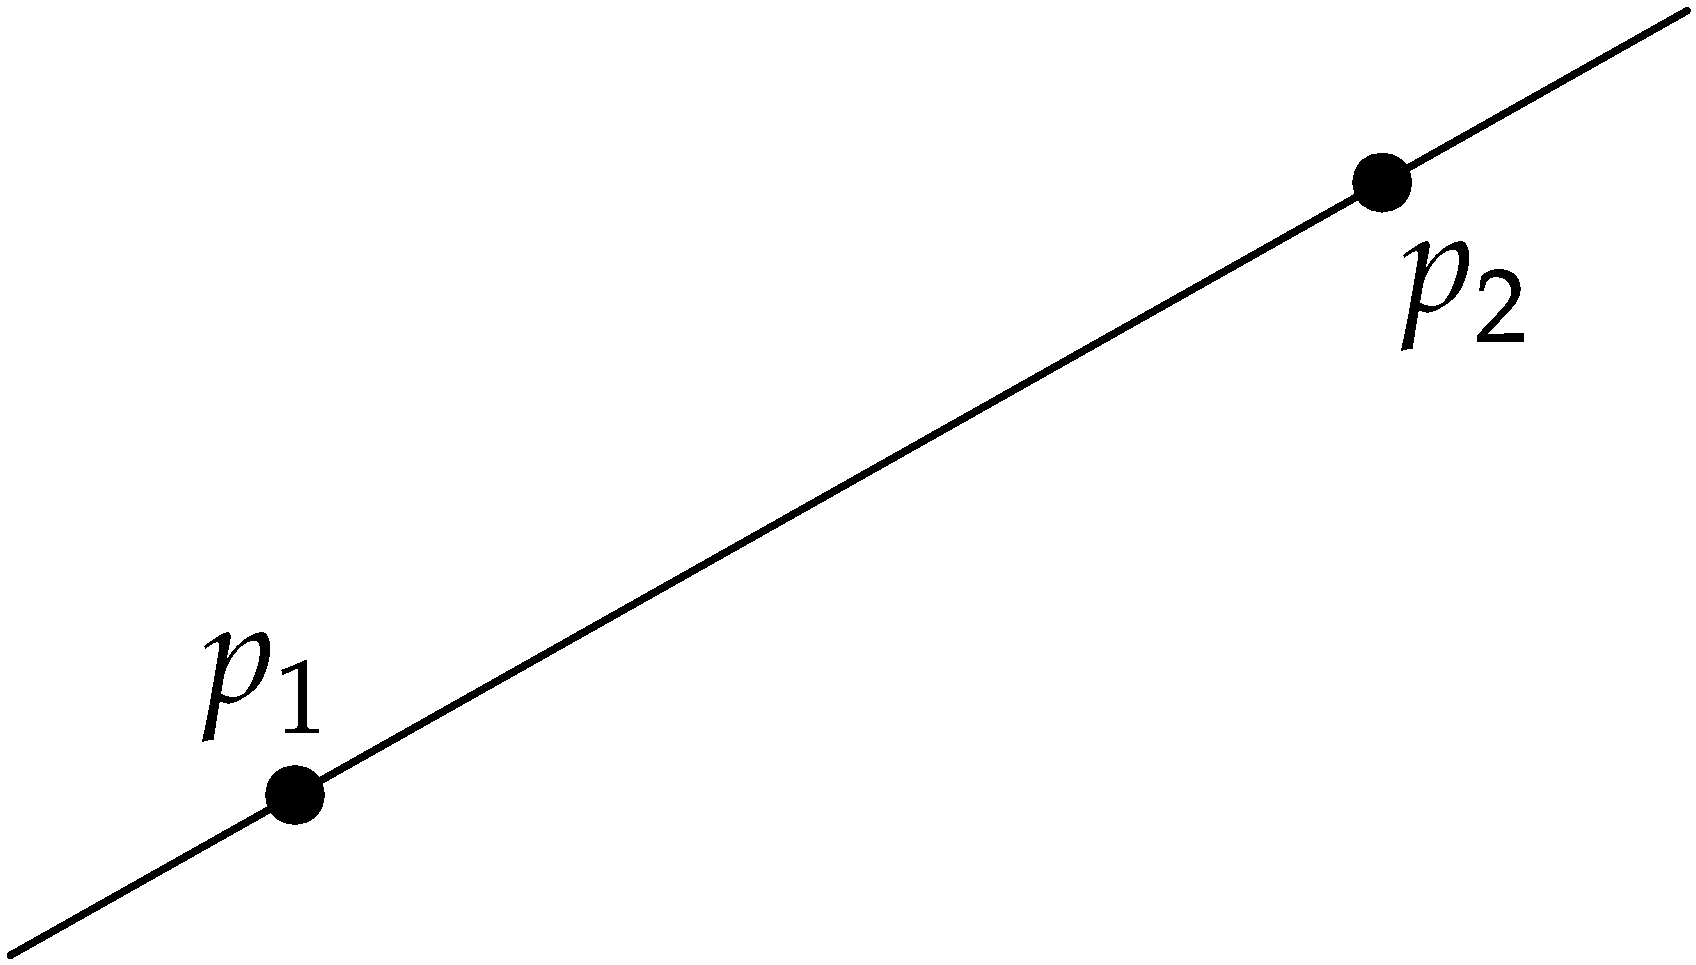
\includegraphics[width=\linewidth]{figs/line.pdf}
\caption{}%
\label{subfig:line}
\end{subfigure}
\quad
\begin{subfigure}[b]{0.3\linewidth}
\includegraphics[width=\linewidth]{figs/loop.pdf}
\caption{}%
\label{subfig:loop}
\end{subfigure}
\caption[Boundary representation]{Boundary representation as applied to: (a) 1D line segments represented implicitly through their two bounding points, and (b) a polygon represented by implying that it is bounded by a set of line segments, which are themselves bounded by consecutive pairs of points in a sequence of points (plus the last and the first).}%
\label{fig:brep}
\end{figure}

Boundary representation works because of what is known in 2D as the Jordan curve theorem\marginnote{Jordan curve theorem}\index{Jordan curve theorem}, which states that a closed curve separates the plane into two parts: an \emph{interior} surface and an \emph{exterior} surface.
In practical terms, this means that if you draw a closed curve (\ie\ a loop) on a sheet of paper, the curve separates the sheet into two parts---an interior one that is bounded on the outside by the curve, and an exterior one that is bounded on the outside by the edges of the sheet (\ie\ its outer boundary) and on the inside by the curve (\ie\ as an inner boundary).
In higher dimensions, this principle is known as the Jordan-Brouwer theorem\marginnote{Jordan-Brouwer theorem}\index{Jordan-Brouwer theorem}, which in 3D says that a closed surface separates 3D space into two parts: an interior volume and an exterior volume.

For our purposes, what the above theorems mean is that if we have a comprehensive method to represent a 2D surface, we can also use it to implicitly represent many 3D volumes with minimal modifications.
The specifics of these modifications depend on the data structure that we are using, but it often is as simple as adding an extra coordinate for each point (\ie\ $(x, y)$ becoming $(x, y, z)$).

\section{Objects with holes}

As hinted in the last paragraph, there are however some 3D volumes that are tricky to store using boundary representation.
The most obvious ones are \emph{objects with 3D holes} (\ie\ cavities)\marginnote{hole}\index{hole}\marginnote{cavity}\index{cavity}, since just like the paper sheet example described previously, they are bounded by one outer surface and possibly several inner surfaces (one per cavity).
Less obviously, objects with 2D faces with holes can have exactly the same problem with certain data structures (Figure~\ref{subfig:hole}), since a surface can be bounded by an outer ring and possibly multiple inner rings.

\begin{figure}
\centering
\begin{subfigure}[b]{0.3\linewidth}
\includegraphics[width=\linewidth]{figs/hole}
\caption{}%
\label{subfig:hole}
\end{subfigure}
\quad
\begin{subfigure}[b]{0.3\linewidth}
\includegraphics[width=\linewidth]{figs/hole-split}
\caption{}%
\label{subfig:hole-split}
\end{subfigure}
\begin{subfigure}[b]{0.3\linewidth}
\includegraphics[width=\linewidth]{figs/hole-bridge}
\caption{}%
\label{subfig:hole-bridge}
\end{subfigure}
\caption[Two different techniques to handle holes]{Two different techniques to handle holes in (a) a volume with 2D faces with holes: (b) splitting the volume into two parts and (c) using a bridge edge.}%
\label{fig:hole}
\end{figure}

Both of these cases are problematic for the same reasons.
In the simplest case, it can be because of a data structure is only built to store one ring/surface (\eg\ a single list of vertices for a ring).
However, the most common issue is that even when multiple rings/surfaces can be stored, the structures representing holes can end up separated from the rest of the data structure, resulting in a \emph{disconnected graph}\marginnote{disconnected graph}\index{disconnected graph}.
In other words, it might be impossible to navigate from the outer boundary of an object to its inner boundaries and vice versa.

While holes can cause problems when modelling objects using boundary representation, these are relatively easy to solve.
The three most common approaches are: 
\begin{enumerate}
	\item splitting volumes into multiple parts in such a manner that the 2D or 3D holes lie between different objects (Figure~\ref{subfig:hole-split}), then somehow semantically marking that the parts belong to the same object (\eg\ by using the same attribute id); 
	\item storing holes just like other (filled) objects, marking them as holes semantically (\eg\ with a special attribute or id), and then storing a list of holes for each object as a sort of attribute, from which they can then be easily accessed;
	\item using one \emph{bridge edge}\marginnote{bridge edge}\index{bridge edge} per hole, which are special edges that join each inner boundary to the outer boundary (Figure~\ref{subfig:hole-bridge}).
	The end result of this approach is that objects are only bounded by a single outer boundary, which wraps around the original outer boundary and all of the former inner boundaries.
	Bridge edges might also be marked semantically as such, although it is possible to tell that an edge is a bridge edge because it is surrounded on all sides by the same 2D/3D object.
\end{enumerate}

% A very similar case to objects with holes are disconnected (\ie\ non-touching) objects, which also result in a disconnected graph.
% In order to support these objects, many data structures have an explicit list of all existing objects, from which it is possible to access them.
% This list can be as simple as an array of pointers or ids, or as complex as a spatial index (\eg\ an R-Tree or $k$-d tree).

\section{Non-manifolds}

In addition to the above mentioned objects with holes, the other kind of objects that are tricky to store using boundary representation are \emph{non-manifolds}\marginnote{non-manifold}\index{non-manifold}.
However, in order to precisely describe what these are, we need to introduce some concepts from topology, which will allow us to describe them in terms of topological characteristics.

Mathematically, a \emph{homeomorphism}\marginnote{homeomorphism}\index{homeomorphism} is a continuous function that also has a continuous inverse.
This is a sort of equivalence relation (\(=\)) in topology, and so it can be used to tell that two objects are topologically equivalent or \emph{homeomorphic}.
In informal terms, applying a homeomorphism is like continuously deforming an object (without making holes in it or glueing different parts of it).
If an object can be transformed to another through this process, they are said to be homeomorphic (Figure~\ref{fig:homeomorphism}).
Homeomorphisms are important because of one key characteristic: they preserve all topological properties.
This means that they can be used to relate an arbitrary object to a simpler well-known one, which then has known topological properties (\eg\ Euclidean 2D space or a sphere).

\begin{figure}[htbp]
\centering
\begin{subfigure}[b]{0.4\linewidth}
\includegraphics[width=\linewidth]{figs/mug}
\caption{}%
\label{subfig:mug}
\end{subfigure}
\quad
\begin{subfigure}[b]{0.4\linewidth}
\includegraphics[width=\linewidth]{figs/donut}
\caption{}%
\label{subfig:donut}
\end{subfigure}
\caption[A typical joke about topology]{A typical joke about topology says that (a) a coffee mug and (b) a donut are homeomorphic.}%
\label{fig:homeomorphism}
\end{figure}

A \emph{manifold}\marginnote{manifold}\index{manifold} is a shape that is homeomorphic to the Euclidean space of a certain dimension, \ie\ a point in 0D, a line in 1D, a plane in 2D or 3D space in 3D.
An intuitive way to think about this is that a manifold locally resembles Euclidean space, even if globally it does not.
For example, a line and a circle are both 1-manifolds, while a plane, a sphere and a torus are all 2-manifolds.
Meanwhile, non-manifolds\marginnote{non-manifold}\index{non-manifold} are shapes where you can find at least one point where this condition is not true (Figure~\ref{subfig:nonmanifold-0} and~\ref{fig:non2manifold}).
In geomatics, when people refer to a non-manifold, they are usually referring to a non-2-manifold in the context of modelling a 3D object using boundary representation.

\begin{figure}
\centering
\begin{subfigure}[b]{0.3\linewidth}
\includegraphics[width=\linewidth]{figs/nonmanifold-0}
\caption{}%
\label{subfig:nonmanifold-0}
\end{subfigure}
\quad
\begin{subfigure}[b]{0.3\linewidth}
\includegraphics[width=\linewidth]{figs/nonmanifold-1}
\caption{}%
\label{subfig:nonmanifold-1}
\end{subfigure}
\quad
\begin{subfigure}[b]{0.3\linewidth}
\includegraphics[width=\linewidth]{figs/nonmanifold-2}
\caption{}%
\label{subfig:nonmanifold-2}
\end{subfigure}
\caption[A 1D boundary around a polygon that is non-1-manifold]{(a) The 1D boundary around a polygon is a non-1-manifold because the space around a vertex (highlighted in a red circle) is not homeomorphic to a line. (b) \& (c) However, the polygon can still be represented using a loop of oriented edges by creating a duplicate vertex at that location (shown as two half disks), but there are two ways in which this can be done.
Note that these are not equally desirable as (c) results in a disconnected structure (just like a hole).}%
\label{fig:nonmanifold}
\end{figure}

Based on these definitions, we can now better describe exactly which 3D objects can be stored using boundary representation without problems: those that are bounded by exactly one 2-manifold surface.
The intuitive logic that explains this is: 2D space is (by definition) a 2-manifold surface, which means that we are able to store objects that are bounded by a surface that is homeomorphic to it.
Another intuitive way to think about this is to consider a counterexample in terms of the Jordan curve theorem: if we draw a closed loop that crosses itself (\eg\ the number 8), which is clearly a non-manifold, we will end up with more than one interior part (or possibly an ambiguous situation).

\begin{marginfigure}
\centering
\includegraphics[width=\linewidth]{figs/non2manifold.jpg}
\caption[A 2D surface around a volume that is non-2-manifold]{The 2D surface around this volume is a non-2-manifold because it is not homeomorphic to a plane.}%
\label{fig:non2manifold}
\end{marginfigure}

While the obvious solution might be to disallow non-manifold objects, they are common in practice, and so we need to have methods to deal with them, even if these methods might introduce additional complexity to boundary representation.
In order to overcome this problem, there are two approaches that are typically used:

\begin{enumerate}
	\item splitting non-manifold objects into multiple manifold parts, then marking the parts as belonging to the same object using semantics;
	\item creating duplicate elements at the same location (Figure~\ref{subfig:nonmanifold-1} and~\ref{subfig:nonmanifold-2}).
		In 2D this usually involves duplicate vertices, whereas in 3D this might involve duplicate edges as well.
\end{enumerate}

\section{Topological concepts}

In addition to holes and manifolds, there are other topological concepts that are commonly used when characterising objects in 3D modelling.
These are not directly related to the present chapter, but we will make a small tangent to introduce them here.

The \emph{genus}\marginnote{genus}\index{genus} of a surface is the maximum number of closed loop cuts we can make in it without causing it to become disconnected (Figure~\ref{fig:genus}).
Note the `maximum' here, since it is always possible to select loops that cause a surface to become disconnected.
Intuitively, it is the number of `handles' it has.
A sphere thus has genus 0, whereas a torus (\eg\ the donut and coffee mug) have genus 1 because we can cut the handle of the object and still have a connected surface.

\begin{figure}
\centering
\begin{subfigure}[b]{0.3\linewidth}
\includegraphics[width=\linewidth]{figs/genus1}
\caption{}%
\label{subfig:genus1}
\end{subfigure}
\quad
\begin{subfigure}[b]{0.3\linewidth}
\includegraphics[width=\linewidth]{figs/genus2}
\caption{}%
\label{subfig:genus2}
\end{subfigure}
\quad
\begin{subfigure}[b]{0.3\linewidth}
\includegraphics[width=\linewidth]{figs/genus3}
\caption{}%
\label{subfig:genus3}
\end{subfigure}
\caption[Surfaces with different genus]{Surfaces with: (a) genus 1, (b) genus 2, (c) genus 3. From Wikimedia Commons.}%
\label{fig:genus}
\end{figure}

A surface is said to be \emph{orientable}\marginnote{orientability}\index{orientability} when it is possible to define a normal vector at every point of the surface in a consistent manner, \ie\ without sudden reversals of the vector direction when moving long the surface.
Since real-world objects are always orientable (Figure~\ref{fig:mobius}), this might seem like a non-issue in practice.
However, real-world objects are always volumetric---no matter how thin they are---but when these are modelled, they are often modelled as surfaces (\ie\ without thickness), which makes it possible to have unorientable surfaces.

\begin{figure}
\centering
\includegraphics[width=0.6\linewidth]{figs/mobius}
\caption[A M\"obius strip]{A M\"obius strip is a one-sided surface, equivalent to glueing a paper strip with a single 180\(^\circ\) twist, and it is the most typical example of a non-orientable surface. Note however that this is only true when it is modelled without thickness. From Wikimedia Commons.}%
\label{fig:mobius}
\end{figure}

\section{Data structures for meshes}

Moving back to the storage of 3D models using boundary representation, there are a large number of data structures that can be used for this purpose.
However, there are three broad approaches: (i) data structures using triangles as base elements; (ii) data structures that use edges or half-edges as base elements; and (iii) data structures that have polygons, edges and vertices as base elements.
We will show one or two characteristic examples for each approach, with the understanding that there are many possible variations of each of them.

\subsection{Triangle-based structures}

The first typical approach relies on a surface being triangulated, \ie\ being split entirely into triangles, so that you have a triangle mesh\marginnote{triangle mesh}\index{triangle mesh}.
This is often desirable because in a triangle mesh, each triangle is known to have only up to three adjacent triangles and only up to three incident vertices, whereas in a polygon it can be any number.
Because of this, a triangle-based data structures (Figure~\ref{fig:2-simplex}) can use fixed-length data structures to store all their elements (\eg\ arrays), which are more efficient.

\begin{figure}
\centering
\begin{subfigure}[b]{0.27\linewidth}
\includegraphics[width=\linewidth]{figs/2-simplex-adjacency}
\caption{}%
\label{subfig:2-simplex-adjacency}
\end{subfigure}
\quad
\begin{subfigure}[b]{0.27\linewidth}
\includegraphics[width=\linewidth]{figs/2-simplex-vertices}
\caption{}%
\label{subfig:2-simplex-vertices}
\end{subfigure}
\quad
\begin{subfigure}[b]{0.27\linewidth}
\includegraphics[width=\linewidth]{figs/0-simplex}
\caption{}%
\label{subfig:0-simplex}
\end{subfigure}
\caption[A triangle-based data structure]{A triangle-based data structure consists of a set of triangles as base elements, each of which has links to (a) its three adjacent triangles (as pointers or ids).
Then, the usual approach is to also have links to (b) its three incident vertices (as pointers or ids), which can stored as separate elements with (c) their coordinates.
Alternatively, it is also possible to store the vertex coordinates directly in the triangles, but this means that the coordinates are stored many times---once in every triangle that is incident to it.}%
\label{fig:2-simplex}
\end{figure}

Since there are specific elements for triangles and vertices, triangle-based data structures make it easy to store attributes both for triangles and for vertices.
For instance, it is possible to mark all the triangles belonging to a certain surface semantically through the use of a common attribute, which could be a pointer or id linking to a surface element.
Such a surface could contain attributes common to all the triangles that represent it.

Surfaces with holes are generally not a problem for triangle-based data structures.
When these are triangulated (using a constrained triangulation), holes become connected to the rest of the structure.
If a hole of a surface contains a different surface, the triangles adjacent to it can simply link to the triangles representing it.
If it does not, the triangles can have a special link or value corresponding to empty space (\eg\ null).
The same applies for triangles on the edge of the surface

In addition to the basic approach, there are variations that use more compact representations of triangle-based structures, usually by joining multiple adjacent triangles that are arranged in a certain way.
Examples of these are triangle strips (Figure~\ref{fig:trianglestrip}) and triangle fans/stars (triangles that are all incident to a certain vertex).

\begin{marginfigure}
\centering
\includegraphics[width=\linewidth]{figs/trianglestrip}
\caption[A triangle strip is easily defined as a list of vertices]{A triangle strip is easily defined as a list of vertices \((a,b,c,d,e,f,g,h)\). Every triangle is formed by three consecutive vertices in the list.}%
\label{fig:trianglestrip}
\end{marginfigure}

\subsection{Edge-based structures}

When we want to allow for polygons in a surface, the most common approach is to use data structures where the base elements are either edges or half-edges.
Let us look at one example of each.

The \emph{quad-edge}\marginnote{quad-edge data structure}\index{quad-edge data structure} data structure uses edges as base elements.
Each edge then stores what is known as a \emph{quad}\marginnote{quad}\index{quad} (Figure~\ref{fig:quad}) and links to one or both of its incident vertices.
Note that these quads are named as such because they store four piece of information and are unrelated to quads (\ie\ quadrilaterals) in computer graphics.

In a common easy implementation of the quad-edge data structure, the edge is first given an arbitrary orientation.
In this manner, there are vertices at the \emph{start} and \emph{end} of the edge, which can be used as names to access them, and there are thus \emph{left} and \emph{right} polygons, which means that the quad links can thus be called something like \emph{left-previous}, \emph{left-next}, \emph{right-previous} and \emph{right-next}.

\begin{figure}[b]
\centering
\includegraphics[width=0.7\linewidth]{figs/quad}
\caption[In the quad-edge data structure, an edge stores a \emph{quad}]{In the quad-edge data structure, an edge stores a \emph{quad}, which contains four records pointing to other quads corresponding to the previous and next oriented edges for the polygons on both of its sides.}%
\label{fig:quad}
\end{figure}

While this approach works fine, it is important to note that there will not be a consistent orientation between adjacent edges.
That is, polygons will not be defined by an oriented loop of edges going around them.
Vertices can thus have multiple edges pointing away from them and toward them.
As an example of the consequences of this, getting all the vertices of a polygon is a bit awkward, since for each iteration where we arrive at an edge, we need to check the orientation of the edge and program a different logic for each orientation.

The alternative is to split each edge into two linked half-edges with opposite orientations.
This approach is called the \emph{half-edge data structure}\marginnote{half-edge data structure}\index{half-edge data structure}, of which are many variations in practice, such as the doubly connected edge list (DCEL)\marginnote{DCEL}\index{DCEL}.
In the DCEL (Figure~\ref{fig:halfedge}), half-edges\marginnote{half-edge}\index{half-edge} are the base element, but there are also elements for vertices and faces.
Vertices store their coordinates and a link to one face-edge starting from it, whereas faces store a link to a half-edge on its outer boundary.
If holes are present, faces also typically store one link to a half-edge on each of its inner boundaries.
Note however that since a face can have any number of holes, this means that a variable-length data structure (\eg\ a linked list) will need to be used.
Vertices, half-edges and faces can each also contain fields for attributes.
Storing attributes for edges will thus result in duplicate information (or additional edge objects that are linked to both half-edges).

\begin{figure}
\centering
\begin{subfigure}[b]{0.27\linewidth}
\includegraphics[width=\linewidth]{figs/halfedge-1}
\caption{}%
\label{subfig:halfedge-1}
\end{subfigure}
\quad
\begin{subfigure}[b]{0.27\linewidth}
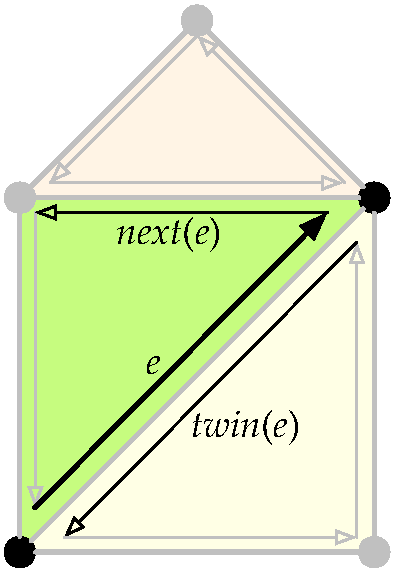
\includegraphics[width=\linewidth]{figs/halfedge-2}
\caption{}%
\label{subfig:halfedge-2}
\end{subfigure}
\caption[Three adjacent polygons are represented using the DCEL]{(a) Three adjacent polygons are represented using (b) the DCEL\@.
In the DCEL, a half-edge \(e\) is linked to two vertices (called the \emph{origin} and the \emph{destination}) and to the face that it is incident to, and is linked to its \emph{next} half-edge (on the same face) and its \emph{twin} half-edge (on the adjacent face).}%
\label{fig:halfedge}
\end{figure}

In general, half-edge data structures are more verbose than edge-based data structures.
However, they make navigating through the structure much easier.
For instance, obtaining all the vertices of a polygon in order in the DCEL simply involves finding a half-edge in the polygon, and then iteratively following the \emph{next} links until we get back to the original half-edge.

\subsection{Incidence graphs}

The last approach that is common in practice is the \emph{incidence graph}\marginnote{incidence graph}\index{incidence graph}.
It is a simple data structure where \(i\)-dimensional elements are linked to the \((i-1)\)-dimensional elements that bound it (Figure~\ref{fig:incidencegraph}).
This approach makes it easy to store attributes for faces, edges and vertices without redundancy.
However, it needs variable-length data structures to store the edges that bound each face.
Because of this, it is commonly used where this limitation is not a problem (\eg\ in text files), but it is avoided when efficiency is more important and where variable-length fields are a problem (\eg\ in databases).

\begin{figure}
\centering
\begin{subfigure}[b]{0.27\linewidth}
\includegraphics[width=\linewidth]{figs/2-cell-boundary}
\caption{}%
\label{subfig:2-cell-boundary}
\end{subfigure}
\quad
\begin{subfigure}[b]{0.27\linewidth}
\includegraphics[width=\linewidth]{figs/1-cell-boundary}
\caption{}%
\label{subfig:1-cell-boundary}
\end{subfigure}
\quad
\begin{subfigure}[b]{0.27\linewidth}
\includegraphics[width=\linewidth]{figs/0-cell-embedding}
\caption{}%
\label{subfig:0-cell-embedding}
\end{subfigure}
\caption[The incidence graph]{In the incidence graph, (a) faces have a list with links to the edges that bound them, (b) edges have links to the two vertices that bound them, and (c) vertices contain their coordinates.}%
\label{fig:incidencegraph}
\end{figure}

%%%
%
\section{Exercises}

\begin{enumerate}
	\item Why can we represent a 2D polygon directly as a sequence of 0D points (\ie\ skipping line segments entirely) but we cannot do the same in 3D\@?
	\item Exactly where is the surface of Figure~\ref{fig:non2manifold} not homeomorphic to a plane?
	\item Splitting objects is a simple solution to deal with both holes and non-manifolds. However, in terms of semantics it is often not desirable. Why is that?
	\item In a triangle fan or star, we need to store vertices in a specific order. Why is that?
	\item How can you obtain all the edges incident to a vertex in order (\ie\ as you rotate around the vertex) using the quad-edge data structure? How about for the DCEL\@? Which is easier?
\end{enumerate}



%%%
%
\section{Notes and comments}

The original place where the Jordan curve theorem is introduced is  \citet{Jordan87}, which is an old French textbook on calculus and differential equations.
The generalisation to higher dimensions was apparently done by \citet{Lebesgue11} and \citet{Brouwer11}, although this is somewhat contentious~\citep[Ch.~5]{van-Dalen13}.

% We mentioned R-trees and \(k\)-d trees as examples of spatial indices.
% The details of each are not very relevant here, but it is good to know that they have tree structures with links to each object in the leaves.
% If you want to get more familiar with them, you can skim the papers where they were introduced, \citet{Guttman84} and \citet{Bentley75}, or simply check the Wikipedia article for an R-tree: \url{https://en.wikipedia.org/wiki/R-tree}.

If you want to see how the coffee mug and the donut from Figure~\ref{fig:homeomorphism} are homeomorphic, watch this video: \url{https://www.youtube.com/watch?v=9NlqYr6-TpA}.

A nice description of a star-based data structure is available in \citet{Blandford05}, or in 3D in \citet{Ledoux13a}.

The quad-edge data structure was originally described in \citet{Guibas85}.
The first data structure of that type is likely the winged-edge data structure~\citet{Baumgart75}.

As for half-edge data structure, the first example is likely the 2D combinational map~\citep{Edmonds60}.
The DCEL is originally described in \citet{Muller78}, but you can find nicer descriptions in \citet{Worboys04} or \citet{deBerg08}.
 % 1.2
% %!TEX root = ../3dbook.tex

\setchapterpreamble[u]{\margintoc}

\graphicspath{{voxels/}}
% \renewcommand*{\thelesson}{2.1}

\chapter{Voxels and voxelisation}%
\label{chap:voxels}

Voxel models, which are the 3D equivalent of 2D rasters, are a common way to store 3D models of the built environment using a regular 3D grid (Figure~\ref{fig:model}).
Much like rasters in 2D, they have inherent limits in precision based on the grid size that is used and can easily grow to very large sizes in terms of memory, especially with a small grid size and when compression is not used.

At the same time, voxel models are easy to use and understand, and algorithms to process them are typically much simpler than those using other representations, which also makes them more reliable, robust and easy to parallelise.
These characteristics make voxels an important and widely used representation to process 3D information in general.

\begin{figure}[htbp]
\centering
\begin{subfigure}[b]{\linewidth}
\includegraphics[width=\linewidth]{figs/model-pre}
\caption{}%
\label{subfig:model-pre}
\end{subfigure}
\\
\begin{subfigure}[b]{\linewidth}
\includegraphics[width=\linewidth]{figs/model-post}
\caption{}%
\label{subfig:model-post}
\end{subfigure}
\caption{(a) A mesh model of a house with surrounding terrain and trees and (b) a corresponding voxel model with the same elements.}%
\label{fig:model}
\end{figure}

\section{Exhaustive enumeration models}

Voxels might appear to be quite a unique data model in terms of 3D representations, but they are actually only the most used among a type of related representations, which are together usually referred to as \emph{exhaustive enumeration}\marginnote{exhaustive enumeration}\index{exhaustive enumeration}.
The specifics of these data models differ, but in general they represent objects by:

\begin{enumerate}

\item \textbf{defining the shape of a domain}\marginnote{voxel domain}\index{voxel domain} in which the objects to be represented fit, or alternatively in which the region of interest of a field fits, \eg\ a bounding box defined by their minimum and maximum coordinates along each axis;

\item \textbf{dividing the domain} using a structure of many \emph{cells}\marginnote{voxel cells}\index{voxel cells}, usually following a regular or semi-regular pattern that can be defined programmatically (as opposed to explicitly representing the shape of each individual cell), \eg\ a grid defined by the number of cells along each axis;

\item \textbf{specifying a well-defined order} passing once through each cell of the subdivision, usually also programmatically (as opposed to explicitly numbering each cell), \eg\ the order and direction of iteration of the axes in a grid;

\item \textbf{labelling each cell} with values that indicate the object(s) that are in it, or in the case of fields, the values of variable(s) at that location.
The values can then be \emph{encoded linearly} using the order defined in the previous step.

\end{enumerate}

We can thus say that what is represented in an exhaustive enumeration is usually composed of four elements: (i) a set of rules defining the shape of a domain, (ii) a set of rules on how to divide the domain into cells, (iii) a set of rules that define an order of the cells, and (iv) an encoded linear representation that represents objects or values for all cells.
However, out of these four elements, the first three are sets of rules that are generally very simple, and thus they are stored encoded in a minimal way or not at all (\ie\ only implied by the context).
For instance, the rules might be part of the specification of a particular data format.

Based on these standard characteristics, we can see that exhaustive enumeration representations use space differently from other data models.
In most geometric representations, much (or most) of the space and complexity of a data structure is devoted to creating a custom structure that individually describes the shape of the objects being represented.
By contrast, in exhaustive enumeration, objects' shapes are instead approximated using simple rules on a predefined structure, and the vast majority of the space is thus devoted to specifying which objects are present in which cells (or the values of a field in each cell).

That being said, the statements described above---which in the steps correspond to the actions that are done for a standard regular 3D grid with voxels---can all differ substantially.
By analysing different possibilities at each step, it is easy to see how the approach can be adapted and extended to form other types of representations.
For instance, consider the following example, which is arbitrarily chosen to be completely different from a typical voxel grid.

We can start by describing a space using an alternative method, \eg\ a b-rep representation of a domain with an arbitrarily complex shape.
Cells could then be specified using a \emph{constrained Delaunay tetrahedralisation} of the domain (using predefined rules for the addition of Steiner points).
The order of the cells could be specified based on the lexicographical order of the vertices of each tetrahedron.
Finally, the values of each tetrahedral cell are then encoded linearly as in a grid.

While the previous example is perfectly possible, it is worth noting that exhaustive enumeration schemes are well-liked largely because of their simplicity, which means that simpler representations are usually preferred.
Using a complex representation where the geometry is not trivial to compute on the fly (\eg\ a CDT) thus defeats many of the advantages of the exhaustive enumeration approach.

Most examples that are found in practice are thus relatively minor variations of voxel grids.
For instance, cells can have varying sizes according to their place in the grid (\eg\ when more details are desired in a particular region), the domains of grids can be stretched in some directions (such that the domain is oblique), or the cells can be of different shapes (\eg\ octahedra).

Among the variations of voxel models, \textbf{sparse voxel models}\marginnote{sparse voxel model}\index{sparse voxel model} are used widely in practice and are thus worth describing in more detail here.
These representations opt to encode only the voxels containing something (rather than all voxels in the domain).
In order to do so, they usually specify simple objects consisting of: (i) a voxel position, \eg\ using integer coordinates for its position along each axis, and (ii) the voxel's variables.
While this is undoubtedly more space-intensive per voxel than the standard encode-all approach, it works well for 3D models consist of largely empty space, which occurs frequently in 3D city models and where the objects we want to represent do not fit neatly into a box-shaped domain.

It is also worth pointing out that most variations of voxel models can be processed with basically the same methods as standard voxel grids.

\section{Hierarchical subdivision models}

In addition to exhaustive enumeration, there are also related data models where the structure is not entirely predefined, but it is instead defined hierarchically using space-partitioning trees.
The root of the tree thus refers to a predefined space that will be subdivided, which corresponds to the entirety of the domain that is represented in an exhaustive enumeration model.
Each node then specifies a subset of the space defined by its parent node, and nodes (usually but not necessarily at the leaf level) are then labelled to specify the object(s) or value(s) present in the space represented by it.

Since different branches of a tree do not need to have the same depth, hierarchical subdivision models can have different resolutions in different parts of the model, and can thus adapt to the shape of the objects being represented.
This allows them to act as more compact alternatives to exhaustive enumeration models in certain cases, usually where there are large objects that occupy many adjoining cells.
Note however that the tree structure of a hierarchical representation can occupy a significant amount of space.

Hierarchical subdivisions are also a good way to encode the sparse models described in the previous section, where large areas of empty space will be efficiently represented by leaf nodes that are generally close to the root of the tree.

The most common structures used by hierarchical subdivision models are:

\begin{description}

\item[octrees] subdivide space evenly along the \(x\), \(y\) and \(z\) axes into eight equal-size \emph{octants}.
They are analogous to quadtrees in 2D, which subdivide space evenly along the \(x\) and \(y\) axes into four equal-size quadrants.

\item[bintrees] are similar to octrees, but they subdivide space in halves along only one axis per node, then switching to a different axis for the next level of the tree, \eg\ \(x\), then \(y\), then \(z\), then \(x\) again, etc.

\item[\(k\)-d trees] are similar to bintrees, but they subdivide space using an arbitrary plane per node, which can be defined by a single coordinate included in the node.

\end{description}

\section{Voxelisation}

The process through which other data models are converted into voxels is called \emph{voxelisation}\marginnote{voxelisation}\index{voxelisation}.
It is analogous to rasterisation in 2D.
In most cases, the data being voxelised consists of vector objects, either as a point cloud or a b-rep mesh.
We will thus explain a method to voxelise 0D, 1D, 2D and 3D vector objects.
In principle, it can be applied to arbitrary curves and surfaces, but in most instances they will be line segments (or polylines), as well as triangular and polygonal meshes.

\subsection{Connectivity}

When rasterising a curve in 2D, different algorithms aim to obtain a pixellated curve that is connected according to either 4-connectivity or 8-connectivity (Figure~\ref{fig:rasterisation}).
These are as follows:
\begin{description}
\item[4-connectivity] means that pixels are connected to their four horizontally and vertically adjacent neighbours.
\item[8-connectivity] means that pixels are connected their four 4-connected neighbours and to their four diagonally incident neighbours.
\end{description}

\begin{figure}
\centering
\includegraphics[width=\linewidth]{figs/rasterisation}
\caption{Rasterising a line to achieve 4-connectivity (left) and 8-connectivity (right). The algorithm uses line targets (orange) that are intersected with the curve.}%
\label{fig:rasterisation}
\end{figure}

In 3D, the equivalent concepts are 6-connectivity, 18-connectivity and 26-connectivity.
These are as follows:
\begin{description}
\item[6-connectivity] \marginnote{6-connectivity}\index{6-connectivity} thus means that voxels are connected to their six adjacent neighbours (\ie\ on their left, right, front, back, bottom and top).
\item[18-connectivity] \marginnote{18-connectivity}\index{18-connectivity} means that voxels are connected to their six 6-connected neighbours and to their twelve incident neighbours that touch them diagonally along an edge (\ie\ top left, top right, top front, top back, bottom left, bottom right, bottom front, bottom back, front left, front right, back left and back right).
\item[26-connectivity] \marginnote{26-connectivity}\index{26-connectivity} means that voxels are connected to their eighteen 18-connected neighbours and to their eight incident neighbours that touch them diagonally along a vertex (\ie\ top front left, top front right, top back left, top back right, bottom front left, bottom front right, bottom back left and bottom back right).
\end{description}

An alternative way to think about these connectivities is that they are defined based on the dimensionality of the common boundary of the pixels or voxels.
6-connectivity means that two neighbouring voxels have a common 2D face.
18-connectivity means that they have at least a common 1D edge (which covers having a common 2D face).
26-connectivity means that they have at least a common 0D vertex (which covers having a common 1D edge or 2D face).

18-connectivity is an interesting concept that shows that there is a consistent logic for every dimension, but it is not really used in practice.
We will thus not discuss it further.

\subsection{Intersections with targets (2D)}

In the example from Figure~\ref{fig:rasterisation}, the pixellated curve is obtained by calculating intersections between the original 1D curve and a set of \emph{intersection targets}\marginnote{intersection target}\index{intersection target} that are 1D line segments.
For 4-connectivity, the targets consist of the four line segments that bound every pixel.
For 8-connectivity, the targets are line segments that bisect the pixel horizontally and vertically and their midpoints.
The intersections with the targets give us a set of points, and the pixels in which these points are tell us the pixels that are part of the pixellated curve.
When a point lies on an edge between two pixels or a vertex between four pixels, we consider that all of the pixels are part of the curve.

In order to understand the logic of the targets, it is important to consider two aspects: (i) where the intersections will lie and (ii) whether they will detect lines when they do not cross the midpoint of a pixel.
For 4-connectivity, the targets simply detect when a line exits the pixel through the left, right, bottom or top edges on the \emph{boundary of the pixel}.
Since all intersections will be between pixels, the 2 or 4 pixels incident to the points will be part of the pixellated curve.
For 8-connectivity, the targets detect when they pass through the middle of the pixel either vertically or horizontally, which happens in the \emph{interior of the pixel}.
Crucially, note that they might do not detect when a line cuts through a corner of the pixel without crossing its middle vertically or horizontally.

Having covered the rasterisation of a 1D curve, let us discuss the two other cases: rasterising 0D points and 2D areas.
Since vector points are not connected, they do not need to be connected when rasterised either.
Since areas are always connected, they should also be connected when rasterised.
Connectivity is thus not an issue, which makes their rasterisation simpler.

An important observation for this method is that we used 1D targets to rasterise a 1D curve.
In order to rasterise a set of 0D points, we would use intersections with 2D targets, of which the optimal choice would consist of the whole area of each 2D pixel.
In order to rasterise a set of 2D areas, we would use intersections with 0D targets, of which the obvious choice is the midpoint of a pixel (although others are possible).
It is possible to see a duality property here: in order to rasterise \(i\)-dimensional objects, we use \((2-i)\)-dimensional targets.

\subsection{Intersections with targets (3D)}

At this point, we should point out that the method described in the previous section is not the absolute fastest or the most common to rasterise objects in 2D.
However, it is a method with good performance with a logic that works perfectly in 3D, which is the reason why we will now explain how it works for voxelisation.

Let us start backwards, with the equivalent duality property for voxelisation, which states that we can use \((3-i)\)-dimensional targets to voxelise \(i\)-dimensional objects.
Using this formula directly, we can discuss the most obvious cases first: voxelising 0D points and 3D volumes, in which connectivity also does not matter.

In order to voxelise \textbf{0D points} (\eg\ a point cloud), we can thus simply use 3D targets that consist of the whole voxel (Figure~\ref{fig:points}).
That is, we can compute for each point which voxel it is in, or for each voxel the points that are in it.
This is a trivial operation using ranges of \(x\), \(y\) and \(z\) coordinates.

\begin{figure}
\centering
\begin{subfigure}[b]{\linewidth}
\includegraphics[width=\linewidth]{figs/points-pre}
\caption{}%
\label{subfig:points-pre}
\end{subfigure}
\\
\begin{subfigure}[b]{\linewidth}
\includegraphics[width=\linewidth]{figs/points-post}
\caption{}%
\label{subfig:points-post}
\end{subfigure}
\caption{A point cloud (a) before and (b) after voxelisation. AHN data from Rotterdam.}%
\label{fig:points}
\end{figure}

Similar to the previous case, in order to voxelise \textbf{3D volumes}, we can use a 0D target with the midpoint of the voxel.
The exact form of this operation depends on the input data.
For instance, if we have tetrahedra as input, it would be a \emph{point in tetrahedron} operation, which could be done using barycentric coordinates.

Now, let us discuss the more challenging cases: 1D and 2D objects.
As with 1D curves in rasterisation, connectivity is important for these, so we will give targets that can be used in order to achieve 6-connectivity and 26-connectivity for each.

In order to voxelise \textbf{1D curves} with 6-connectivity (Figure~\ref{fig:lines}), we could detect when these pass through the top, bottom, left, right, front or back faces of the voxel using 2D targets (Figure~\ref{subfig:1d6}).
For 26-connectivity, we could detect when these pass through the middle of the voxel using three bisecting faces (Figure~\ref{subfig:1d26}).

\begin{figure}
\centering
\begin{subfigure}[b]{\linewidth}
\includegraphics[width=\linewidth]{figs/lines-pre}
\caption{}%
\label{subfig:lines-pre}
\end{subfigure}
\\
\begin{subfigure}[b]{\linewidth}
\includegraphics[width=\linewidth]{figs/lines-post}
\caption{}%
\label{subfig:lines-post}
\end{subfigure}
\caption{A set of lines (a) before and (b) after voxelisation. OpenStreetMap data from Istanbul.}%
\label{fig:lines}
\end{figure}

\begin{figure}
\centering
\begin{subfigure}[b]{0.45\linewidth}
\includegraphics[width=\linewidth]{figs/1d6}
\caption{}%
\label{subfig:1d6}
\end{subfigure}
\quad
\begin{subfigure}[b]{0.45\linewidth}
\includegraphics[width=\linewidth]{figs/1d26}
\caption{}%
\label{subfig:1d26}
\end{subfigure}
\caption{Intersection targets (blue) for 1D curves for (a) 6-connectivity and (b) 26-connectivity.}%
\label{fig:1d}
\end{figure}

Now, in order to voxelise \textbf{2D surfaces} (Figure~\ref{fig:surfaces}) with 6-connectivity, we can use 1D targets that detect when we pass through any of the 12 edges on the boundary of the voxel (Figure~\ref{subfig:2d6}).
For 26-connectivity, we can use 1D targets that detect when we pass through the middle of the voxel (Figure~\ref{subfig:2d26}).

\begin{figure}
\centering
\includegraphics[width=\linewidth]{figs/surfaces}
\caption{Voxelising a surface}%
\label{fig:surfaces}
\end{figure}

\begin{figure}
\centering
\begin{subfigure}[b]{0.45\linewidth}
\includegraphics[width=\linewidth]{figs/2d6}
\caption{}%
\label{subfig:2d6}
\end{subfigure}
\quad
\begin{subfigure}[b]{0.45\linewidth}
\includegraphics[width=\linewidth]{figs/2d26}
\caption{}%
\label{subfig:2d26}
\end{subfigure}
\caption{Intersection targets (black lines) for 2D surfaces for (a) 6-connectivity and (b) 26-connectivity.}%
\label{fig:2d}
\end{figure}

%%%
%
\section{Exercises}

\begin{enumerate}
	\item Can you devise a formula to compare the space occupied by:
	\begin{enumerate}
		\item encoding all voxels in a grid linearly
		\item using a sparse encoding with individual voxels
		\item using a sparse encoding with an octree
	\end{enumerate}
	\item Can you think of cases where the rasterisation targets for 1D lines do not work? Hint: think of short curves.
	\item What kind of connectivity is used in the example of Figure~\ref{fig:lines}?
\end{enumerate}



%%%
%
\section{Notes and comments}

Voxels are widely used in areas other than geographic information.
For instance, both medical magnetic resonance (MRI) and computer tomography (CT) scans produce voxel models.
Physical simulations also use voxels since many calculations are easy to do using regular grid structures, \eg\ finite-element analysis.
Games sometimes use voxels as well, both for calculations and to render graphics.
It is worth noting that many of the techniques developed in these fields are just as applicable to geographic information as well.

4D grids using 3D+time are also sometimes used, both in geographic information and elsewhere.
Some of the earliest papers to mention this are: \citet{Mason94}, who implemented a system using a 4D grid of ocean temperatures with support for interpolation and generalisation operations, and \citet{Bernard98}, who implemented a 4D grid of atmospheric variables (\eg\ temperature, wind or pollution), which can be used for simulations.

A common use of the representations covered here, especially voxel grids and octrees, is spatial indexing.
Cells can thus be used to store other kinds of data, \eg\ ids of objects, memory addresses with data, or a subset of a point cloud.

The original paper describing quadtrees is \citet{Finkel74}, whereas that for octrees is \citet{Meagher80}.
Bintrees~\citep{Samet85} are an alternative that split dimensions alternately rather than all at once.
If you are curious about more types of trees used in hierarhical subdivisions, have a look at the section titled `Spatial data partitioning trees' in this Wikipedia template: \url{https://en.wikipedia.org/wiki/Template:CS_trees}.

The voxelisation algorithm covered here is described by \citet{Laine13}, although it might be easier to understand the implementation described in \citet{Nourian16}.
Alternative targets to the ones described in this lesson are shown in both papers.
 % 2.1
% %!TEX root = ../3dbook.tex

\setchapterpreamble[u]{\margintoc}

\graphicspath{{LoD2recon/}}
% \renewcommand*{\thelesson}{2.2}

\chapter{3D building reconstruction}%
\label{chap:LoD2recon}

%\newpage
In the previous lesson we discussed how to model 3D objects using the boundary representation.
You learned about data structures to represent the geometry and topology of a 3D object's surface in a very structured and organised way.
In this lesson we will look at how you could create such a structured representation from a much less structured form of 3D geoinformation, namely a point cloud.

In automatic building reconstruction we aim to construct 3D mesh models for individual buildings from some form of elevation measurements, \ie\ a raster-based DSM or a point cloud, without any manual interventions (see Figure~\ref{fig:bk-building-recon}).
\begin{marginfigure}
	\centering
	\begin{subfigure}{\linewidth}
		\includegraphics[width=\linewidth]{figs/bk-pointcloud.png}
		\caption{}%
		\label{subfig:bk-pc}
	\end{subfigure}
\\
	\begin{subfigure}{\linewidth}
		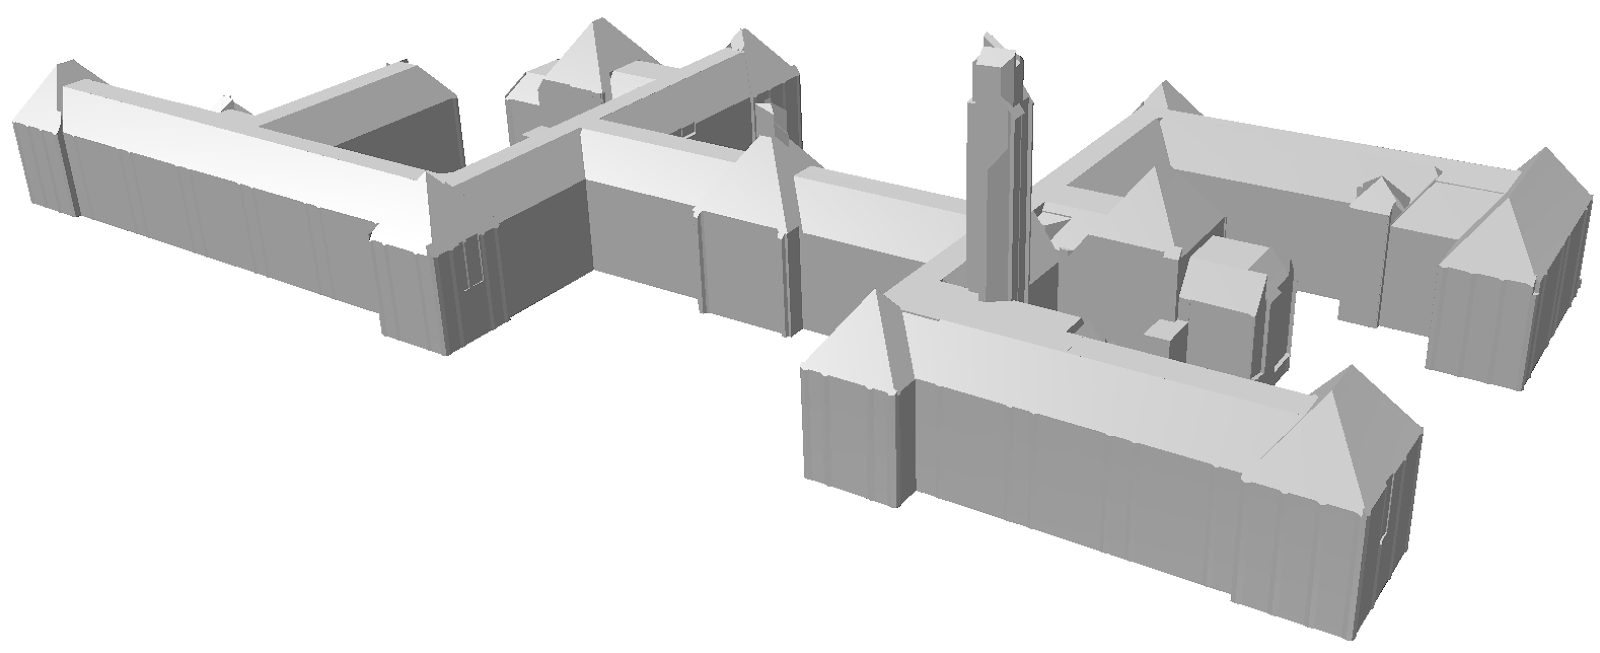
\includegraphics[width=\linewidth]{figs/bk-mesh.png}
		\caption{}%
		\label{subfig:bk-mesh}
	\end{subfigure}
	\caption{Building reconstruction transforms a point cloud (a) into a mesh model (b).}%
	\label{fig:bk-building-recon}
\end{marginfigure}
It can be considered as one step in the geoinformation chain, since we essentially transform 'raw' and unorganised point measurements into more structured and semantically rich 3D models.
Compared to a point cloud, such models are much more useful for applications such as environmental simulations of wind, air pollution, and noise propagation, but also building energy demand estimation and urban planning in general.
Many of these applications require knowledge about the volume or surface area of a building, or the distinction between the interior and exterior of a building, which is evidently much easier to derive from a mesh with a clearly defined boundary than from a point cloud.
In addition, meshes are typically more compact which makes them more efficient to store and process.

This is not to say that meshes are always superior to point clouds. 
For example some of the finer details that may be present in a point cloud could be lost in the mesh representation. 
Furthermore, there is always the risk of introducing new errors and deviations from the original measurement in the building reconstruction process. 
But ultimately, the many benefits of representing a building as a mesh outweigh these disadvantages for many applications.

In this lesson we will first list common challenges and requirements for the building models that are to be constructed. Second, we will look at the important engineering choices in designing a building reconstruction algorithm. And finally, we will discuss one particular approach that was designed to work on Dutch open data in more detail.

%%%
%
\section{Building model requirements and reconstruction challenges}
When designing a building reconstruction method, it is important to carefully consider both the \emph{model requirements} and the \emph{reconstruction challenges}. 
The model requirements specify in detail what properties a reconstructed building model should have. 
Model requirements are mostly application dependent.
For example, an application that performs heavy geometric processing on the building models has stricter geometry and topology requirements than an application that merely visualises the building models.
Reconstruction challenges, on the other hand, are mostly input dependent. 
It is about the characteristics of the input data and the typical shape of the buildings that are present in the input data.
It is relatively easy to design a reconstruction approach for a very high quality point cloud that contains only very simple building shapes, whereas reconstructing complex building shapes from a very sparse and low quality input point cloud is substantially more difficult.

\subsection{Building model requirements}
Following are commonly encountered building model requirements. Notice that the exact requirements will depend on the application.
%An ideal reconstruction method would satisfy all these requirement, but note that in practice we often encounter models that fail in one or several of these.

\begin{description}
	\item[Low complexity] Means that the building model ought to have as few vertices, edges, and faces as possible. Building models with a low complexity are faster to process and take up less storage space.
	\item[High accuracy] The surfaces of the building model should have the lowest possible error with respect to the input point cloud. This error can be measured as the root mean square of all the distances from each input point to the model surface. 
	\item[Geometrically valid] This means among other things that the mesh is 2-manifold, has consistent faces orientation, no duplicated vertices, and no self intersecting geometries. This makes the model generally easier to process since many assumptions can be made about the structure of the mesh. Lesson 3.2 discusses this (and the relevant ISO19107 standard) in more detail.
	\item[Level of Detail (LoD)] Specifies the degree of generalisation in the roof structure of the reconstructed building model when compared to how the actual building is built. An LoD1 model for example only allows horizontal flat roof surfaces (even if the actual building roof looks different), whereas an LoD2 model also allows for more detailed multi-pitched roof shapes. For the remainder of this lesson we will focus on the more detailed LoD2 models. Lesson 4.1 discusses the possible LoDs for building models in more detail.
\end{description}

\subsection{Reconstruction challenges}
Why can it be hard to satisfy the model requirements? This depends on the reconstruction challenges. We distinguish between two main categories.

Firstly, there are variations in architectural style. Urban environments can be complex and organised with a high degree of randomness due to their anarchical creation over time. This makes it difficult to design a reconstruction algorithm that is able to model 100\% of the buildings on earth. It is probable that there are always a few cases that violate some of the assumptions made in the building reconstruction method. For example, to simplify a reconstruction approach, it may seem reasonable to assume that buildings are not built on top of each other without touching each other. And while this assumption is valid in more than 99\% of the cases, in practice there are some violations of this assumption (see Figure~\ref{fig:debrug}).
\begin{figure}
	\centering
	\includegraphics[width=\linewidth]{figs/de_brug.jpg}
	\caption{A complex urban environment.}%
	\label{fig:debrug}
\end{figure}
	
Secondly, we need to consider the quality and completeness of the input data. This mostly relates to how the input data, \ie\ the point cloud, was acquired (compare \eg\ Figure~\ref{fig:pc-quality:low} to \ref{fig:pc-quality:high}).
\begin{marginfigure}
	\centering
	\begin{subfigure}{\linewidth}
		\includegraphics[width=\linewidth]{figs/rdam16_ahn2.png}
		\caption{}%
		\label{fig:pc-quality:low}
	\end{subfigure}
	\\
	\begin{subfigure}{\linewidth}
		\includegraphics[width=\linewidth]{figs/rdam16_d.png}
		\caption{}%
		\label{fig:pc-quality:high}
	\end{subfigure}
	\caption{Varying point cloud qualities. a) low point density with missing facades, b) high point density and points on facades.}%
	\label{fig:pc-quality}
\end{marginfigure}
Most building reconstruction methods work with point clouds that are captured from an airplane. 
This is the most efficient way to cover large areas, but it also means that not all the exterior surfaces of a building are captured due to occlusion. In particular facades and the underside of overhanging structures may be missing in such datasets. 
If a surface is missing in the point cloud we need to compensate for that with assumptions on what we expect the building to look like. 
For instance, we could assume that facades are always vertical so that we can simply model a vertical plane from the roofline to the ground. 
However, while this is reasonable for the majority of buildings there are bound to be some exceptions.
Other point cloud properties are also important. For example the point density is indicative for the smallest details that we can reliably detect in the point cloud. Consequently we can not reasonably expect to see smaller details in the reconstructed building model unless very strong assumptions are taken on the type of building shape that is modelled. Some surface materials can also lead to problems. Glass surfaces for example are notoriously difficult to measure with airborne acquisition techniques, leading \eg\ to holes in the roof surface which can lead to problems in a building reconstruction method.


%%%
%
\section{Data driven versus model driven building reconstruction}
Building reconstruction has been a popular topic among researcher over the last few decades. 
Many approaches exist that vary in the expected type and resolution or density of input data, the precise model requirements, and in how restricted they are to a particular architectural style.
One could classify these methods on a linear scale with on one extreme the purely so-called \emph{data  driven} approaches and on the other extreme the purely so-called \emph{model driven} approaches.

\begin{marginfigure}
	\includegraphics[width=\linewidth]{figs/data-driven.png}
	\caption{Data driven reconstruction based on a triangulation of the input points \citep{Axelsson99}}%
	\label{subfig:data-driven}
\end{marginfigure}
The data driven approach strongly relies on the quality and completeness of the input data.
The resulting building models have a good data fit, but a high complexity (high number of faces).
Defects in the input data are likely to cause problems in the building model, such as holes and non-2-manifoldness.
Examples of the data driven approach are methods that triangulate directly the input point cloud (see Figure~\ref{subfig:data-driven}).

\begin{marginfigure}
	\includegraphics[width=\linewidth]{figs/model-driven.png}
	\caption{Model driven reconstruction by fitting parametrised roof models \citep{Lafarge10}}%
	\label{subfig:model-driven}
\end{marginfigure}
The model driven approach, on the other hand, relies on strong modelling assumptions about the building shape.
This typically results in models with a low complexity, but a poorer fit with the input points when compared to a purely data driven approach.
Because the model driven approach does not rely so heavily on the quality of the input, defects in the input point cloud are less likely to lead to problems in the building model.
Examples of the model driven approach are methods that fit pre-defined roof shapes such as a simple gable roof to a point cloud (see Figure~\ref{subfig:data-driven}). 
Such a method will only work for buildings for which a pre-defined roof shape is available.
Yet, if this the case it can already work reliably for a very sparse point cloud.

Clearly both approaches have limitations. The most advanced building reconstruction methods, including the one discussed below, try to combine the best of both to come to an optimal compromise, \eg\ a method that has both a good datafit and a high degree of flexibility in building shapes but also a low complexity and perfect geometric validity. However, be aware that such a mixed approach combines not only the advantages, but likely also the disadvantages of both approaches to some degree.

% Table~\ref{tab:data-vs-model-driven} gives an overview of the various trade-offs between the data driven and the model driven approach. 
% \begin{table}[]
% 	\centering
% 	\begin{tabular}{p{7cm}|p{7cm}}
% 	Data driven & Model driven \\
% 	\hline
% 	Requires high quality input	& Suitable for low quality input \\
% 	Good data fit	& Possibly loose data fit \\
% 	Sensitive to defects in input data &  Can overcome input defects to some extent \\
% 	High model complexity & Low model complexity \\
% 	No assumptions on building shape	&  Strong assumptions on building shape\\
% 	Can deal with large variety of building shapes	& Limited to specific building shapes\\
% 	No semantics (\ie\ no distinction roof, wall and floor faces) & Has semantics
% 	\end{tabular}
% 	\caption{Trade-offs in data driven versus model driven reconstruction}%
% 	\label{tab:data-vs-model-driven}
% \end{table}
% Notice that this table describes merely the two extremes, and that mixed approaches also exist.
%The important thing is that you learn to understand about the 


%In conclusion, it should be clear that there is no such thing as a perfect . 

% model only superstructures with model-driven approach (iconisation)


\section{Automatic LoD2 reconstruction for the Netherlands}
% design context
In this section we will discuss an automatic LoD2 reconstruction method that I developed to work with Dutch open data\footnote{the AHN3 point cloud and the BAG building footprints}. 
The output of this method should have both a good data fit and a low model complexity and is aimed to have completely valid geometry output. 
This means the resulting models are suitable for various kinds of environmental simulation applications.

% modelling assumptions
\subsection{Modelling assumptions}
The following assumptions are taken in the reconstruction method. They are deemed reasonable for the Dutch input datasets that the method was designed on, and with these assumption the reconstruction problem is somewhat simplified.

\begin{description}
	\item[piecewise planar] The shape of a building can be adequately approximated using planar faces that are detectable from the point cloud.
	\item[2.5D with vertical walls] The roof of the building is 2.5D and all walls are vertical. This implies the 3D building model can be extruded from a 2D planar partition of the roof. The 2.5D assumption is quite reasonable for airborne point cloud, because each building is only scanned from above anyhow.
	\item[classified point cloud] A reliable classification of the input point cloud is expected, \ie\ at least a building and a terrain (ground) class must be present. This is the case for the AHN3 dataset that is used.
	\item[footprints are available] Apart from a point cloud the method also takes 2D building footprints as input. These are used to crop the point cloud for each building. It is assumed that the footprints are up-to-date and well aligned with the point cloud.
\end{description}

% data or model driven?
The method can be classified as a mix between the purely data and model driven approaches as discussed in the previous section. 
Consequently it also mixes the benefits and trade-offs of both extremes.
For example, instead of forcing complete roof shapes on a point cloud, it is only assumed a building is composed of planar surfaces.
This makes the method more flexible compared to a purely model driven approach that fits a pre-defined roof shape, since it should be able to handle any possible roof shape that can reasonably be approximated with (large) planar surfaces while still mainting a low model complexity.
However, if a plane cannot be fitted to a part of the roof due to defects in the point cloud, that part may lead to errors in the resulting building model.


% overview method
\subsection{Method overview}
Figure~\ref{fig:method-overview} illustrates the six main steps of the algorithm. The main idea is to compute a so-called \emph{roof-partition}; a planar partition of the footprint where each face corresponds to a planar piece of the roof and is labeled with a roof plane. Prior to creating the roof-partition the roofplane and line features must be extracted from the point cloud (Figure~\ref{fig:method-overview} step 2 and 3). And once the roof-partition is available, the 3D building model can be generated through extrusion (Figure~\ref{fig:method-overview} step 6).
\begin{figure}
	\centering
	\includegraphics[width=\linewidth]{figs/reconstruction-overview.pdf}
	\caption{The main steps in the reconstruction algorithm. 1) the classified (aerial) point cloud is cropped on the 2D footprint, 2) planes and their boundaries are detected in the point cloud, 3) from the roof planes the intersection lines and boundary lines are extracted, 4) the lines are regularised and projected onto the 2D footprint, 5) the roof-partitions is created. This is a DCEL where each face is labeled with the corresponding plane (from 2, compare colors). 6) the roof-partition is extruded into a 3D mesh. \\If a terrain plane is assigned to a face from the roof-partition, that face is removed (2 and 5).}%
	\label{fig:method-overview}
\end{figure}

%The method consists of five steps.
%\begin{enumerate}
%	\item Plane detections
%	\item Line detection and regularisation
%	\item Subdivision of the footprint
%	\item Graph-cut optimisation
%	\item Extrusion
%\end{enumerate}

\subsubsection{Feature extraction}
% \begin{kaobox}[frametitle=\faExternalLink\ To read or to watch.]
% 		The reader is advised to read the section on shape detection in the Chapter \emph{Point cloud processing} in the book \href{https://github.com/tudelft3d/terrainbook/releases}{\emph{Computational modelling of terrains}}.
% \end{kaobox}
The roof-partition is made using lines that are derived from roof planes that are extracted from the building point cloud.
The roof planes are detected using a region-growing algorithm and then two type of lines are derived from the planes: boundary lines and intersection lines (see Figure~\ref{fig:method-overview} step 3).
The boundary lines are created by detecting lines in the boundary of the $\alpha$-shape of each detected roof plane.
The intersection lines are created where adjacent planes intersect, such as on the top of a gable roof.

Before the boundary and intersection lines are used to partition the footprint, they are regularised.
The goal of line regularisation is to remove duplicate lines and thereby reduce the complexity of the roof-partition.
For example, the line on top of the gable roof in Figure~\ref{fig:method-overview} is detected three times: once as an intersection line and twice as a boundary line (once for each incident roof plane).
After line regularisation only a single line remains.
After projecting the detected lines to 2D, line regularisation is done in two steps: orientation clustering and distance clustering (see Figure~\ref{fig:lineclust}).

Orientation clustering is performed first, and in this step lines that have approximately the same orientation in the 2D plane are put in the same cluster. For example in Figure~\ref{fig:lineclust:2}, there are two dominant orientations that each form a cluster of lines. Withing each orientation cluster the angle between the lines is relatively small, whereas the angle between lines in different clusters is large.
\begin{figure}
	\centering
	\begin{subfigure}[b]{0.48\linewidth}
		\includegraphics[angle=90,width=\linewidth]{figs/line-clustering/slice1.pdf}
		\caption{Detected lines}%
		\label{fig:lineclust:1}
	\end{subfigure}
	\quad
 	\begin{subfigure}[b]{0.48\linewidth}
		\includegraphics[angle=90,width=\linewidth]{figs/line-clustering/slice2.pdf}
		\caption{Orientation clustering}%
		\label{fig:lineclust:2}
	\end{subfigure}
\\
	\begin{subfigure}[b]{0.48\linewidth}
		\includegraphics[angle=90,width=\linewidth]{figs/line-clustering/slice3.pdf}
		\caption{Distance clustering}%
		\label{fig:lineclust:3}
	\end{subfigure}
\quad
	\begin{subfigure}[b]{0.48\linewidth}
		\includegraphics[angle=90,width=\linewidth]{figs/line-clustering/slice4.pdf}
		\caption{Regularised lines}%
		\label{fig:lineclust:4}
	\end{subfigure}	
	\caption{Line regularisation through clustering. }%
	\label{fig:lineclust}
\end{figure}

Next, distance clustering is performed.
This divides each orientation cluster into one or more distance clusters.
This is done by computing for each orientation cluster the distances between the lines it contains.
Groups of lines with a small distance with respect to each other are put in their own distance cluster, weheras the distance between different distance clusters is large (see Figure~\ref{fig:lineclust:3}).

Finally, one average line is computed for each distance cluster (Figure~\ref{fig:lineclust:4}).

\subsubsection{Construction of the roof-partition}
After the lines are detected and regularised they are used to subdivide the footprint into a planar partition called the roof-partition.
A doubly connected edge list (DCEL) is used to represents the full topology of the planar partition of the footprint, that is referred to as the \emph{initial roof-partition}.
This means that each intersection is explicitly represented with a vertex.
In addition there are no dangling edges.
The use of a DCEL allows for easy traversal and manipulation of the roof-partition, \eg\ for the extrusion to a 3D mesh in the last step.


Depending on the number of lines that remain after regularisation, the initial roof-partition may still have a high complexity; it may contain many small faces.
To further reduce the complexity of the roof-partition and to simultaniously assign an optimal roofplane to each face, an optimisation step is performed\footnote{Graph-cut optimisation is used. The details on how graph-cut optimisation works are outside the scope of this course.}.
In this step a roof plane is assigned to each face in the roof-partition (see Figure~\ref{fig:method-overview} step 5).
This is done in such a way that 1) the total error with the input point cloud is minimised and 2) the total length of the edges between faces of a different roof plane is minimised.
This  optimisation thus seeks an optimal balance between respectively a good data fit and a low complexity of the roof-partition.
After the optimisation is complete, the edges for which the two incident faces are assigned to the same roof plane are removed from the partition.
The faces in the resulting \emph{final roof-partition} are referred to as \emph{roof-parts}.

\subsubsection{Extrusion}
\label{sec:extrusion}
The final roof-partition is transformed into a 3D building mesh using extrusion.
This is done by exploiting the topological information that is available in the the DCEL of the roof-partition, as illustrated in Figure~\ref{fig:extrusion}.
\begin{figure}
	\centering
	\begin{subfigure}[b]{0.45\linewidth}
		\includegraphics[width=\linewidth]{figs/2DDCEL.pdf}
		\caption{}%
		\label{subfig:2ddcel}
	\end{subfigure}
	\quad
	\begin{subfigure}[b]{0.45\linewidth}
		\includegraphics[width=\linewidth]{figs/3DDCEL.pdf}
		\caption{}%
		\label{subfig:3ddcel}
	\end{subfigure}
	\caption{The roof-partition is represented as a DCEL (a). When extruding to a 3D mesh (b), each edge in the roof-partition becomes a wall face in the 3D Mesh. Each vertex in the roof-partition (\eg\ $v_1$) needs to be replicated for each incident face: \eg\ $v_{1A}$, $v_{1B}$, $v_{1C}$ in the 3D Mesh.}%
	\label{fig:extrusion}
\end{figure}
Notice that the building mesh consists of three types of faces, \ie\ the floor, the roof and the wall faces.
These are generated from the roof-partition in separate procedures.

\begin{marginfigure}
	\centering
	\includegraphics[width=\linewidth]{figs/extrusion-edge.pdf}
	\caption{The edge $e$ (comprising of two halfedges $e_A$ and $e_B$) is incident to two faces ($f_A$ and $f_B$) and two vertices ($v_1$ and $v_2$). In case of a roof-partition, the height at $v_1$ on face $f_A$ is denoted as $h_{1A}$.}%
	\label{fig:extrusion-notation}
\end{marginfigure}

\begin{description}
\item[floor face] The geometry of the floor face consists of the edges in the roof-partition that are incident to the exterior to the footprint. The elevation of the floor face can either be set to the lowest ground point around the building, or if a terrain mesh is available it can be made exactly fitting with the terrain by computing the intersection with that terrain mesh and setting the vertex elevations accordingly. 

\item[wall faces] These are vertical faces that connect the floor face with the roof faces. They are extruded from the edges in the roof-partition that have one or two incident roof parts. Depending on the plane configuration of the incident roof parts an edge is extruded differently. Figure~\ref{fig:extrusion-cases} shows a few possible cases (there are more).
\begin{figure}
	\includegraphics[width=\linewidth]{figs/extrusion-edge-cases.pdf}
	% \caption{Various possible roof face configurations at edge $e$}%
	\caption{Determining wall face geometry and vertex order. $h_{1A}$ denotes the elevation at vertex $v_1$ on face $f_A$ (see Figure~\ref{fig:extrusion-notation}).}%
	\label{fig:extrusion-cases}
\end{figure}
Notice that an edge in the roof-partition can generate 0 (if the incident planes intersect exactly at the edge), 1 or 2 wall faces.
Also notice that the order of the vertices of a wall face (so that they are oriented counter-clockwise around the face normal that points to the exterior of the mesh) is completely determined by the plane configuration case at the edge.

Special attention needs to be paid to vertices that are extruded to more than two elevations such as $v_1$ in Figure~\ref{subfig:2ddcel}.
To get a topologically correct building mesh, the extruded vertices should become part of all their incident wall faces.
Vertex $v_{1B}$ should thus also be inserted in the boundary ring of the blue face in Figure~\ref{subfig:3ddcel}, despite the fact it is co-linear with $v_{1A}$ and $v_{1C}$.

\item[roof faces]  Each roof part in the interior of the roof-partition will generate a roof face in the building mesh. The planimetric geometry of the roof faces is identical to the faces in the roof-partition. The vertex elevations are found by projecting the 2D vertices to the plane of the roof-part.
\end{description}

%%%
%
\section{Notes and comments}
\citet{Rottensteiner14} gives an overview of building reconstruction methods.

If you want to know more about the graph-cut optimisation method to optimise the roof-partition have a look at the paper from \citet{Zebedin08}.

A good example of a true 3D building reconstruction method (no 2.5D assumption) is the work of \citet{Nan2017}

%%%
%
\section{Exercises}

\begin{enumerate}
  \item Explain the advantages of 2-manifoldness in a building model
  \item Complete the table of possible plane configurations in Figure~\ref{fig:extrusion-cases}.
  \item Could a non-manifold edge be created in the extrusion that is described in Section~\ref{sec:extrusion}? If so, describe how that could happen.
\end{enumerate}
 % 2.2
% %!TEX root = ../3dbook.tex
% chktex-file 46
% chktex-file 36

\setchapterpreamble[u]{\margintoc}

\graphicspath{{dtvd3d/}}
% \renewcommand*{\thelesson}{3.1}

\newcommand{\Orient}{O\textsc{rient}\xspace}
\newcommand{\Insphere}{I\textsc{n}S\textsc{phere}\xspace}

\chapter[Tetrahedralisations and 3D Voronoi diagrams]{Tetrahedralisations and \\3D Voronoi diagrams}%
\label{chap:dtvd3d}


The Delaunay triangulation (DT) and the Voronoi diagram (VD) are fundamental data structures when dealing with spatial datasets, many computer scientists and mathematicians consider the VD as being the most fundamental spatial structure (or spatial model) because it is very simple, and yet is so powerful that it helps in solving many theoretical problems, as well as many real-world applications.

The DT and the VD are most often presented, described, and used, in two dimensions, but their concepts can be generalised to higher dimensions.
We describe in this chapter the concepts in $\mathbb{R}^{3}$, and also discuss the $n$-dimensional cases when appropriate.%
\index{Euclidean space}\marginnote{three-dimensional Euclidean space}

We also discuss how the constrained and conforming DT can be generalised to $\mathbb{R}^{3}$.

\begin{kaobox}[frametitle=\faExternalLink\ To read or to watch.]
  The reader is advised to first read the Chapter \emph{Triangulations \& Voronoi diagram} in the book \emph{Computational modelling of terrains}~\citep{terrain_book}, where the 2D concepts are introduced.
\end{kaobox}

%%%
%
\section[3D Voronoi diagram]{The three-dimensional Voronoi Diagram}

Let $S$ be a set of points in $\mathbb{R}^d$. 
The Voronoi cell of a point $p \in S$, defined $\mathcal{V}_{p}$, is the set of points $x \in \mathbb{R}^d$ that are closer to $p$ than to any other point in $S$; that is:
\begin{equation}
\mathcal{V}_p = \{x \in \mathbb{R}^{d} \ | \ \|x-p\| \, \leq \, \|x-q\|, \ \forall \, q \in S \} 
\end{equation}
The union of the Voronoi cells of all generating points $p \in S$ form the Voronoi diagram of $S$, defined VD($S$). 
If $S$ contains only two points $p$ and $q$, then VD($S$) is formed by a single hyperplane defined by all the points $x \in \mathbb{R}^d$ that are equidistant from $p$ and $q$. 
This hyperplane is the perpendicular bisector of the line segment from $p$ to $q$, and splits the space into two (open) half-spaces. 
\index{half-space}
$\mathcal{V}_p$ is formed by the half-space containing $p$, and $\mathcal{V}_q$ by the one containing $q$. 

%

As shown in Figure~\ref{fig:halfspaces}, 
\begin{marginfigure}
  \centering
  \includegraphics[width=0.8\textwidth]{figs/halfspaces}
  \caption{The Voronoi cell $\mathcal{V}_p$ is formed by the intersection of all the half-planes between $p$ and the other points.}%
\label{fig:halfspaces}
\end{marginfigure}
when $S$ contains more than two points (let us say it contains $n$ points), the Voronoi cell of a given point $p \in S$ is obtained by the intersection of $n-1$ half-spaces defined by $p$ and the other points $q \in S$. 
That means that $\mathcal{V}_{p}$ is always convex, in any dimensions. Notice also that every point $x \in \mathbb{R}^d$ has at least one nearest point in $S$, which means that VD($S$) covers the entire space.

%

As shown in Figures~\ref{fig:vd2d}, 
\begin{marginfigure}
  \centering
  \includegraphics[width=0.8\textwidth]{figs/vd2d}
  \caption{The VD for a set $S$ of points in the plane (the black points).}%
\label{fig:vd2d}
\end{marginfigure}
the VD of a set $S$ of points in $\mathbb{R}^2$ is a planar graph, but it can also be seen as a two-dimensional cell complex where each 2-cell is a (convex) polygon. 
Two Voronoi cells, $\mathcal{V}_{p}$ and $\mathcal{V}_{q}$, lie on the opposite sides of the perpendicular bisector separating the points $p$ and $q$. 

%

In $\mathbb{R}^3$, VD($S$) is a three-dimensional cell complex. 
The Voronoi cell of a point $p$ is formed by the intersection of all the half-spaces (three-dimensional planes) between $p$ and the other points in $S$. 
Drawing a picture of the three-dimensional case is not easy, thus Figure~\ref{fig:vd3d} shows two adjacent Voronoi cells (which are convex polyhedra), and Figure~\ref{fig:vd3d_onecell} one cell with its incident Delaunay edges.
\begin{marginfigure}
  \centering
  \includegraphics[width=0.8\textwidth]{figs/vd3d}
  \caption{Two Voronoi cells adjacent to each other in $\mathbb{R}^3$, they share the grey face.}%
\label{fig:vd3d}
\end{marginfigure}
\begin{marginfigure}
  \centering
  \includegraphics[width=\textwidth]{figs/vd3d_onecell}
  \caption{The Voronoi cell for the red vertex, the red edges are the Delaunay edges that are dual to the Voronoi facets.}%
\label{fig:vd3d_onecell}
\end{marginfigure}

%

The VD has many properties, and most of them are valid in any dimensions. 
Note that most of these properties are valid only when the set $S$ of points is in \emph{general position}, that is when for example in three dimensions no five points are cospherical, and no four points are collinear. 
Details concerning the possible degeneracies are given in Section~\ref{sec:degeneracies}. 
What follows is a list of the most relevant properties:
\begin{description}
  \item[Size:] if $S$ has $n$ points, then VD($S$) has exactly $n$ Voronoi cells since there is a one-to-one mapping between the points and the cells.
  \item[Voronoi vertices:] in $\mathbb{R}^d$, a Voronoi vertex is equidistant from ($d+1$) points. In $\mathbb{R}^3$, a Voronoi vertex is at the centre of a sphere defined by 4 points in $S$.
  \item[Voronoi edges:] in $\mathbb{R}^d$, a Voronoi edge is equidistant from $d$ points.
  \item[Voronoi faces:] in $\mathbb{R}^d$, a Voronoi face is equidistant from ($d-1$) points. Hence, in $\mathbb{R}^3$, it is the bisector plane perpendicular to the line segment joining two points.
  \item[Convex hull:] let $S$ be a set of points in $\mathbb{R}^d$, and $p$ one of its points. $\mathcal{V}_{p}$ is unbounded if $p$ bounds conv($S$). Otherwise, $\mathcal{V}_{p}$ is the convex hull of its Voronoi vertices. 
\end{description}


%%%
%
\section[Delaunay tetrahedralisation]{The Delaunay tetrahedralisation}

The Delaunay triangulation of a set $S$ of points in $\mathbb{R}^d$ is a simplicial complex where each $d$-simplex $\sigma$, formed by $d+1$ vertices in $S$, has an empty \emph{circumball} (a ball is said to be \emph{empty} when no points are in its interior). 
\begin{marginfigure}
  \centering
  \includegraphics[width=\textwidth]{figs/dt2d_2}
  \caption{The DT of a set of points in the plane.}%
  \label{fig:dt2d_2}
\end{marginfigure}
For $\mathbb{R}^3$, it is called the \emph{Delaunay tetrahedralisation}: the space is tessellation into non-overlapping tetrahedra having an empty \emph{circumsphere} (as shown in Figure~\ref{fig:dt3d}).
\begin{marginfigure}
  \centering
  \includegraphics[width=0.8\textwidth]{figs/dt3d}
  \caption{A Delaunay tetrahedron has an empty circumsphere.}%
\label{fig:dt3d}
\end{marginfigure}


%%%
\subsection{Duality between the DT and the VD}

The VD and the DT are dual to each other, and that in any dimensions.
This means they represent the same thing but from a different point-of-view, and one structure can always be extracted from the other.
Consider a graph embedded in $\mathbb{R}^{d}$ as a $d$-dimensional cell complex. 
The mappings between the elements of a cell complex in $\mathbb{R}^{d}$ are as follows: let $C$ be a $k$-cell, the dual cell of $C$ in $\mathbb{R}^{d}$ is denoted by $C^{\star}$ and is a ($d-k$)-cell. 

%

The duality between the VD and the DT in $\mathbb{R}^3$ are thus as follows: 
\begin{figure}
  \centering
  \includegraphics[width=1.0\textwidth]{figs/duality_3d}
  \caption{Duality in $\mathbb{R}^{3}$ between the elements of the VD and the DT.}%
\label{fig:duality_3d}
\end{figure}
\begin{itemize}
  \item a Delaunay vertex $p$ becomes a Voronoi cell (Figure~\ref{fig:duality_3d}a); 
  \item a Delaunay edge $\alpha$ becomes a Voronoi face (Figure~\ref{fig:duality_3d}b);
  \item a Delaunay triangular face $\kappa$ becomes a Voronoi edge (Figure~\ref{fig:duality_3d}c);
  \item a Delaunay tetrahedron $\tau$ becomes a Voronoi vertex (Figure~\ref{fig:duality_3d}d). 
\end{itemize}
A Voronoi vertex is located at the centre of the sphere circumscribed to its dual tetrahedron, and two vertices in $S$ have a Delaunay edge connecting them if and only if their two respective dual Voronoi cells are adjacent.


%%%
\subsection{Convex Hull}
In any dimensions, the DT of set $S$ of points subdivides completely conv($S$), \ie\ the union of all the simplices in DT($S$) is conv($S$).
The boundary of a convex hull in 3D is formed of a set of triangles.
Figure~\ref{fig:dt2}b shows an example.
\begin{figure*}
  \centering
  \begin{subfigure}[b]{0.29\linewidth}
    \includegraphics[width=\textwidth]{figs/t1}
    \caption{}
  \end{subfigure}%
  \qquad
  \begin{subfigure}[b]{0.29\linewidth}
    \includegraphics[width=\textwidth]{figs/t2}
    \caption{}
  \end{subfigure}%
  \qquad
  \begin{subfigure}[b]{0.29\linewidth}
    \includegraphics[width=\textwidth]{figs/t3}
    \caption{}
  \end{subfigure}%
  \caption{\textbf{(a)} A set of 1000 points randomly distributed in a cube. \textbf{(b)} Its convex hull. \textbf{(c)} The Delaunay tetrahedralisation of the points, `sliced' in the middle and the upper tetrahedra removed (to be able to visualise the interior).}%
\label{fig:dt2}
\end{figure*}


%%%
\subsection{Local Optimality}
Let $\mathcal{T}$ be a triangulation of $S$ in $\mathbb{R}^d$. 
A facet $\sigma$ 
\index{facet}\marginnote{facet}
(a ($d-1$)-simplex) is said to be \emph{locally} Delaunay if it either:
\begin{description}
  \item[(i)] belongs to only one $d$-simplex, and thus bounds conv($S$), or
  \item[(ii)] belongs to two $d$-simplices $\sigma_a$ and $\sigma_b$, formed by the vertices of $\sigma$ and respectively the vertices $a$ and $b$, and $b$ is outside of the circumball of $\sigma_a$.
\end{description}
The second case is illustrated in two dimensions in Figure~\ref{fig:slivers}a. 
\begin{figure}
  \centering
  \includegraphics[width=0.9\textwidth]{figs/slivers}
  \caption{\textbf{(a)} A four-sided convex polygon $abcd$ can be triangulated in two different ways, but the empty circumcircle criterion guarantees that the triangles are as equilateral as possible. Notice that the edge $ac$ is not locally Delaunay, but $bd$ is. \textbf{(b)} In three dimensions, five vertices can be triangulated with either two or three tetrahedra. Although the tetrahedralisation at the bottom has two nicely shaped tetrahedra, they are not Delaunay (the point $d$ is inside the sphere $abce$, which also implies that $b$ is inside the sphere $acde$). The tetrahedralisation at the top respects the Delaunay criterion, but contains one very thin tetrahedron spanned by the points $a$, $b$, $d$ and $e$.}%
\label{fig:slivers}
\end{figure}
In an arbitrary triangulation, not every facet that is locally Delaunay is necessarily a facet of DT($S$), but local optimality implies globally optimality in the case of the DT:
\begin{quote}
  Let $\mathcal{T}$ be a triangulation of a point set $S$ in $\mathbb{R}^d$. If every facet of $\mathcal{T}$ is locally Delaunay, then $\mathcal{T}$ is the Delaunay triangulation of $S$.
  \marginnote{locally Delaunay}
\end{quote}
This has serious implications as the DT---and its dual---are locally modifiable, \ie\ we can theoretically insert, delete or move a points in $S$ without recomputing DT($S$) from scratch.


%%%
\subsection{Angle Optimality}
The DT in two dimensions has a very important property that is useful in applications such as finite element meshing or interpolation: the \emph{max-min angle optimality}.
\marginnote{max-min angle optimality}\index{max-min angle optimality}
Among all the possible triangulations of a set $S$ of points in $\mathbb{R}^2$, DT($S$) maximises the minimum angle (max-min property), and also minimises the maximum circumradii. 
In other words, it creates triangles that are as equilateral as possible. 

%

Finding `good' tetrahedra, \ie\ nicely shaped, is however more difficult than finding good triangles because the max-min property of Delaunay triangles does not generalise to three dimensions. 
A DT in $\mathbb{R}^3$ can indeed contain some tetrahedra, called \emph{slivers}, 
\marginnote{slivers}\index{slivers}
whose four vertices are almost coplanar (see Figure~\ref{fig:slivers}b); these tetrahedra are Delaunay. 
Note that such slivers do not have two-dimensional counterparts.

%

For many applications where the Delaunay tetrahedralisation is used, \eg\ in the finite element method in engineering or when the tetrahedra are used to perform interpolation directly, these tetrahedra are bad and must be removed. 
Why use the DT in three dimensions then?
First, it should be said that in most cases Delaunay tetrahedra have in general a more desirable shape than arbitrary tetrahedra, they tend to favour `round' tetrahedra. 
Second, the VD is not affected by them: Voronoi cells in three dimensions will still be `relatively spherical' even if the DT has many slivers. 
Third, if the VD is used for interpolation, then the VD is necessary because many GIS operations use the properties of the VD (see Section~\ref{sec:interpol}), and if only one tetrahedron does not have an empty circumsphere, then the VD is corrupted.



%%%
\subsection{Lifting on the paraboloid}%
\label{sec:parabolic_lifting}

There exists a close relationship between DTs in $\mathbb{R}^{d}$ and convex polytopes in $\mathbb{R}^{d+1}$. 

Let $S$ be a set of points in $\mathbb{R}^{d}$, and let $x_{1}, x_{2}, \ldots , x_{d}$ be the coordinates axes. 
The parabolic lifting map projects each vertex $v(v_{x1}, v_{x2}, \ldots , v_{xd})$ to a vertex $v^{+}(v_{x1}, v_{x2}, \ldots , v_{xd}, v_{x1}^{2}+v_{x2}^{2}+\cdots+v_{xd}^{2})$ on the paraboloid of revolution in $\mathbb{R}^{d+1}$. 
The set of points thus obtained is denoted $S^{+}$. 
Observe that, for the two-dimensional case, the paraboloid in three dimensions defines a surface whose vertical cross sections are parabolas, and whose horizontal cross sections are circles; the same ideas are valid in higher dimensions. 

%

The relationship is the following: every facet (a $d$-dimensional simplex) of the lower envelope of conv($S^{+}$) projects to a $d$-simplex of the Delaunay triangulation of $S$. 
This is illustrated in Figure~\ref{fig:paraboloid} for the construction of the DT in $\mathbb{R}^{2}$. 
\begin{marginfigure}
  \centering
  \includegraphics[width=0.95\textwidth]{figs/paraboloid}
  \caption{The parabolic lifting map for a set $S$ of points $\mathbb{R}^2$.}%
\label{fig:paraboloid}
\end{marginfigure}

%

In short, the construction of the $d$-dimensional DT can be transformed into the construction of the convex hull of the lifted set of points in ($d+1$) dimensions.
In practice, since it is easier to construct convex hulls (especially in higher dimensions, \ie\ 4+), the DT is often constructed with this method.


%%%
\subsection{Degeneracies}%
\label{sec:degeneracies}

The previous definitions of the VD and the DT assumed that the set $S$ of points is in general position, \ie\ the distribution of points does not create any ambiguity in the two structures. 
For the VD/DT in $\mathbb{R}^{d}$, the degeneracies, or special cases, occur when $d+1$ points lie on the same hyperplane and/or when $d+2$ points lie on the same ball. 
For example, in three dimensions, when five or more points in $S$ are cospherical there is an ambiguity in the definition of DT($S$). 
This implies that DT($S$) is not unique; VD($S$) is still unique, but it has different properties.


%%%
%
\section[Construction of 3D DT/VD]{Construction of the 3D DT/VD}

As is the case in 2D, there exist several algorithms to construct either the DT or the VD from a set of points in 3D.

%

Mainly three paradigms of computational geometry can be used for computing a Delaunay triangulation in two and three dimensions:  divide-and-conquer, sweep plane, and incremental insertion.
In two dimensions, each one of these paradigms yields an optimal algorithm.
In three dimensions, things are a bit more complicated.
Divide-and-conquer algorithms have a worst time complexity of $\mathcal{O}(n^3)$, although in practice they are subquadratic.
Only incremental insertion algorithms have a complexity that is worst-case optimal, \ie\ $\mathcal{O}(n^2)$ since the complexity of the DT in $\mathbb{R}^3$ is quadratic.
That is, there are configurations of $n$ points that yield a DT with $\mathcal{O}(n^2)$ tetrahedra.

%

And as is the case in 2D, it is often simpler to reconstruct and store the DT (because they have only 4 vertices and 4 neighbours) and to extract the VD on-the-fly when needed.

%

The details of the algorithms are out of scope for this course.
We provide in the following a general idea of how the reconstruction of the DT is performed in 3D by generalising the algorithm described in GEO1015.

\begin{kaobox}[frametitle=\faCog\ How does it work in practice?]
  Even more than in 2D, the duality between the convex hull in $d+1$-dimension and the DT in $d$-dimension is in practice exploited.
  Indeed, one can construct the convex hull of a set of points projected to 4D to obtain the DT in 3D.
  One popular and widely used implementation is Qhull (\url{http://www.qhull.org/}).
\end{kaobox}


%%%
\subsection{Generalisation of the flip-based incremental insertion algorithm}

The algorithm described in Algorithm~\ref{algo:insert1pt} is a generalisation to 3D of the flip-based incremental insertion algorithm used for 2D DT\@.
\begin{algorithm}[tb] 
  \DontPrintSemicolon\
  \KwIn{A DT($S$) $\mathcal{T}$ in $\mathbb{R}^3$, and a new point $p$ to insert}
  \KwOut{$\mathcal{T}^{p} = \mathcal{T} \cup \{p\}$}
  find tetrahedron $\tau$ containing $p$\;
  insert $p$ in $\tau$ by splitting it in to 4 new tetrahedra (flip14)\;
  push 4 new tetrahedra on a stack\;
  \While{stack is non-empty}
  {
    $\tau = \{p,a,b,c\} \leftarrow$ pop from stack\;
    $\tau_{a} = \{a,b,c,d\} \leftarrow$ get adjacent tetrahedron of $\tau$ having the edge $abc$ as a face\;
    \If{$d$ is inside circumsphere of $\tau$}
    {
      \If{configuration of $\tau$ and $\tau_a$ allows it}
      {
        flip the tetrahedra $\tau$ and $\tau_{a}$ (flip23 or flip32)\;
        push 2 or 3 new tetrahedra on stack\;
      }
      \Else{Do nothing} 
    }
  }
  \caption{Algorithm to insert one point in a DT}%
\label{algo:insert1pt}
\end{algorithm} 

Most steps can be generalised in a direct way.
Figure~\ref{fig:insertion_steps} shows the steps from the 2D algorithm, which are conceptually the same for the 3D generalisation of the algorithm (and it is more difficult to draw these steps in 3D).
\begin{figure*}
  \centering
  \includegraphics[width=1.5\textwidth]{figs/insertion_steps}
  \caption{Step-by-step insertion, with flips, of a single point in a DT in two dimensions.}%
\label{fig:insertion_steps}
\end{figure*}




As is the case with the two-dimensional algorithm, the point $p$ is first inserted in $\mathcal{T}$ with a flip (\emph{flip14} in the case here), 
\marginnote{flips}\index{flip14}
and the new tetrahedra created must be tested to make sure they are Delaunay. 
The sequence of flips needed is controlled by a stack containing all the tetrahedra that have not been tested yet. 
The stack starts with the four resulting tetrahedra of the \emph{flip14}, and each time a flip is performed, the new tetrahedra created are added to the stack. 
The algorithms stops when all the tetrahedra incident to $p$ are Delaunay, which also means that the stack is empty.


%%%
\paragraph{Initialisation: the big tetrahedron.}
A DT is initialised with a tetrahedron several times larger than the spatial extent of $S$.
The points in $S$ are therefore always added inside an existing tetrahedron. 

%%%
\paragraph{Walk/Point location.}
To find the tetrahedron containing the newly inserted point $p$, the adjacency relationships between the tetrahedra can be used. 
With a series of \Orient\ tests one can navigate from one tetrahedron to the other.

%%%
\paragraph{Flips.}
A flip is a local (topological) operation that modifies the configuration of some adjacent tetrahedra. 
In 2D, for 4 points, a flip (called \emph{flip22}), modifies the configuration of 2 adjacent triangles by flipping the diagonal of the quadrilateral.
In 3D, there are 2 kinds of flips: \emph{flip23} and \emph{flip32}.
Consider the set $S = \{a, b, c, d, e\}$ of points in general position in $\mathbb{R}^{3}$ and its convex hull conv($S$). 
There exist two possible configurations, as shown in Figure~\ref{fig:flips3d}:
\begin{marginfigure}
  \centering
  \includegraphics[width=\textwidth]{figs/flips3d}
  \caption{The 4 different kinds of flips in 3D.}% 
\label{fig:flips3d}
\end{marginfigure}
\begin{enumerate}
  \item the five points of $S$ lie on the boundary of conv($S$); see Figure~\ref{fig:flips3d}a. There are exactly two ways to tetrahedralise such a polyhedron: either with two or three tetrahedra. In the first case, the two tetrahedra share a triangular face $bcd$, and in the latter case the three tetrahedra all have a common edge $ae$.
  \item one point $e$ of $S$ does not lie on the boundary of conv($S$), thus conv($S$) forms a tetrahedron; see Figure~\ref{fig:flips3d}b. The only way to tetrahedralise $S$ is with four tetrahedra all incident to $e$.
\end{enumerate}
Based on these two configurations, four types of flips in $\mathbb{R}^{3}$ can be described: \emph{flip23}, \emph{flip32}, \emph{flip14} and \emph{flip41} (the numbers refer to the number of tetrahedra before and after the flip). 
When $S$ is in the first configuration, two types of flips are possible: a \emph{flip23} is the operation that transforms one tetrahedralisation of two tetrahedra into another one with three tetrahedra; and a \emph{flip32} is the inverse operation. 
If $S$ is tetrahedralised with two tetrahedra and the triangular face $bcd$ is not locally Delaunay, then a \emph{flip23} will create three tetrahedra whose faces are locally Delaunay. 

A \emph{flip14} refers to the operation of inserting a vertex inside a tetrahedron, and splitting it into four tetrahedra; and a \emph{flip41} is the inverse operation that deletes a vertex.

Flips can not always be applied during an insertion, it depends on the local configuration.
For example, in Figure~\ref{fig:flips3d}a, a \emph{flip23} is possible on the two adjacent tetrahedra $abcd$ and $bcde$ if and only if the line $ae$ passes through the triangular face $bcd$ (which also means that the union of $abcd$ and $bcde$ is a convex polyhedron). 
If not, then a \emph{flip32} is possible if and only if there exists in the tetrahedralisation a third tetrahedron adjacent to both $abcd$ and $bcde$.



%%%
\subsection{Predicates}

The `orientation' of points in three dimensions is somewhat tricky because, unlike in two dimensions, we can not simply rely on the counter-clockwise orientation. 
In three dimensions, the orientation is always relative to another point of reference, \ie\ given three points we cannot say if a fourth one is left of right, this depends on the orientation of the three points.
When dealing with a single tetrahedron $\tau$ formed by the four vertices $a$, $b$, $c$ and $d$ (as in Figure~\ref{fig:orient}), 
\begin{marginfigure}
  \centering
  \includegraphics[width=0.9\textwidth]{figs/orient}
  \caption{The tetrahedron $abcd$ is correctly oriented since \Orient($a,b,c,d$) returns a positive result. The arrow indicates the correct orientation for the face $\sigma_a$, so that \Orient($\sigma_a,a$) returns a positive result.}%
\label{fig:orient}
\end{marginfigure}
we say that $\tau$ is correctly oriented if \Orient($a,b,c,d$) returns a positive value. 
Notice that if two vertices are swapped in the order, then the result is the opposite (\ie\ \Orient($a,c,b,d$) returns a negative value). 

Vertices forming a face in a tetrahedron $\tau$ can also be ordered. 
As shown in Figure~\ref{fig:orient}, a face $\sigma_a$, formed by the vertices $b$, $c$ and $d$, is correctly oriented if \Orient($\sigma_a,a$) gives a positive result---in the case here, \Orient($b,c,d,a$) gives a negative result, therefore the correct orientation of $\sigma_a$ is $cbd$. Observe that the face $bcd$ is called $\sigma_a$ because it is `mapped' to the vertex $a$ that is opposite; each of the four faces of a tetrahedron can be referred to in this way.

\Orient\ determines if a point $p$ is over, under or lies on a plane defined by three points $a$, $b$ and $c$.
It returns a positive value when the point $p$ is above the plane defined by $a$, $b$ and $c$; a negative value if $p$ is under the plane; and exactly 0 if $p$ is directly on the plane.
\Orient\ is consistent with the left-hand rule: when the ordering of $a$, $b$ and $c$ follows the direction of rotation of the curled fingers of the left hand, then the thumb points towards the positive side (the above side of the plane). 
In other words, if the three points defining a plane are viewed clockwise from a viewpoint, then this viewpoint defines the positive side the plane.

\Orient\ can be implemented as the determinant of a matrix:
\begin{equation}
  \textrm{O}\textsc{rient}(a, b, c, p) = 
  \left| 
  \begin{array}{cccc}
    a_{x} & a_{y} & a_{z} & 1 \\
    b_{x} & b_{y} & b_{z} & 1 \\
    c_{x} & c_{y} & c_{z} & 1 \\
    p_{x} & p_{y} & p_{z} & 1 
  \end{array} 
  \right| 
\end{equation}
%


The predicate \Insphere\ follows the same idea: a positive value is returned if $p$ is inside the sphere; a negative if $p$ is outside; and exactly 0 if $p$ is directly on the sphere. 
Observe that to obtain these results, the points $a$, $b$, $c$ and $d$ in \Insphere\ must be ordered such that \Orient($a,b,c,d$) returns a positive value. 

It should be noticed that \Insphere\ is derived from the parabolic lifting map (see Section~\ref{sec:parabolic_lifting}). 
It is simply transformed into a four-dimensional \Orient\ test: $p$ is inside (outside) the sphere $abcd$ if and only if $p^{+}$ lies under (above) the hyperplane $a^{+}b^{+}c^{+}d^{+}$, and directly on the sphere if $p^{+}$ lies on the hyperplane $a^{+}b^{+}c^{+}d^{+}$.

\begin{equation}
  \textrm{I}\textsc{n}\textrm{S}\textsc{phere}(a, b, c, d, p) = 
  \left| 
  \begin{array}{ccccc}
    a_{x} & a_{y} & a_{z} & a^{2}_{x} + a^{2}_{y} + a^{2}_{z} & 1 \\
    b_{x} & b_{y} & b_{z} & b^{2}_{x} + b^{2}_{y} + b^{2}_{z} & 1 \\
    c_{x} & c_{y} & c_{z} & c^{2}_{x} + c^{2}_{y} + c^{2}_{z} & 1 \\
    d_{x} & d_{y} & d_{z} & d^{2}_{x} + d^{2}_{y} + d^{2}_{z} & 1 \\
    p_{x} & p_{y} & p_{z} & p^{2}_{x} + p^{2}_{y} + p^{2}_{z} & 1 
  \end{array} 
  \right|%
\label{eq:insphere}
\end{equation}


%%%
\subsection{Data structure} Instead of storing triangles as the atom, tetrahedra are used, they have 4 pointers to their 4 vertices, and 4 pointers to their 4 adjacent tetrahedra.
All of them must be oriented correctly (as is the case in 2D where they are all counter-clockwise), as defined above.


%%%
\subsection{Extracting the VD from the DT}%
\label{sec:extraction_vddt}

Let $\mathcal{T}$ be the DT of a set $S$ of points in $\mathbb{R}^3$. 
The simplices of the dual $\mathcal{D}$ of $\mathcal{T}$ can be computed as follows (all the examples refer to Figure~\ref{fig:duality_3d}):
\begin{itemize}
  \item \textbf{Vertex:} a single Voronoi vertex is easily extracted---it is located at the centre of the sphere passing through the four vertices of its dual tetrahedron $\tau$.
  \item \textbf{Edge:} a Voronoi edge, which is dual to a triangular face $\kappa$, is formed by the two Voronoi vertices dual to the two tetrahedra sharing $\kappa$.
  \item \textbf{Face:} a Voronoi face, which is dual to a Delaunay edge $\alpha$, is formed by all the vertices that are dual to the Delaunay tetrahedra incident to $\alpha$. The idea is simply to `turn' around a Delaunay edge and extract all the Voronoi vertices. These are guaranteed to be coplanar, and the face is guaranteed to be convex.
  \item \textbf{Polyhedron:} the construction of one Voronoi cell $\mathcal{V}_{p}$, dual to a vertex $p$, is similar: it is formed by all the Voronoi vertices dual to the tetrahedra incident to $p$. Since a Voronoi cell is convex by definition, it is possible to collect all the Voronoi vertices and then compute the convex hull; the retrieval of all the tetrahedra incident to $p$ can be done by performing a breadth-first search-like algorithm on the graph dual to the tetrahedra. A simpler method consists of first identifying all the edges incident to $p$, and then extracting the dual face of each edge.
\end{itemize}
Given $\mathcal{T}$, we must obviously visit all its 3-simplices to be able to extract $\mathcal{D}$. This means that computing $\mathcal{D}$ from $\mathcal{T}$ has a complexity of $\Theta(n)$ when $S$ contains $n$ points.





%%%
%
\section[Applications]{Applications of the DT and the VD}
% TODO : section about applications of the 3D VD/DT?
  % - relationships in 3D between points
  % - interpolation of 3D samples
  % - FEM
  % - surface reconstruction
  % - iso-surfaces



%%%
\subsection{Modelling continuous 3D fields (as an alternative to voxels)}

The objects studied in geoscience are often not man-made objects, but rather the spatial distribution of three-dimensional continuous geographical phenomena such as the salinity of a body of water, the humidity of the air, or the percentage of gold in the rock. 
These are referred to as fields, and raster structures (voxels or octrees) are the most popular solutions for modelling them.
However, using regular structures has shortcomings and therefore the VD is a viable alternative.

One advantage is that the VD will adapt to the anisotropic distribution of the samples collected to study a field, these samples are three-dimensional points ($x,y,z$) to which an attribute is attached (\eg\ the percentage of a certain mineral in a body of water).
In practice, the samples can be very hard and expensive to collect because of the difficulties encountered and the technologies involved. 
To collect samples in the ground we must dig holes or use other devices (\eg\ ultrasound penetrating the ground); underwater samples are collected by instruments moved vertically under a boat, or by automated vehicles; and samples of the atmosphere must be collected by devices attached to balloons or aircraft. 
As shown in Figure\ref{fig:watercolumns}, samples are often abundant vertically but very sparse horizontally. 
\begin{figure*}
  \centering
  \begin{subfigure}[b]{0.38\linewidth}
    \centering
    \includegraphics[width=\textwidth]{figs/watercolumns1.pdf}
    \caption{}
  \end{subfigure}%
  \qquad
  \begin{subfigure}[b]{0.45\linewidth}
    \centering
    \includegraphics[width=\textwidth]{figs/watercolumns2.pdf}
    \caption{}
  \end{subfigure}
\caption{\textbf{(a)} Example of a dataset in geology, where samples were collected by drilling a hole in the ground. Each sample has a location in 3D space ($x-y-z$ coordinates) and one or more attributes attached to it. \textbf{(b)} An oceanographic dataset in the Bering Sea in which samples are distributed along water columns. Each red point represents a (vertical) water column, where samples are collected every 2m, but water columns are about 35km from each other.}%
\label{fig:watercolumns}%
\end{figure*}

Another advantage is that the VD can be efficiently and robustly reconstructed, and that based on it the samples can be interpolated to obtain an estimation of the attribute at any location, see below for details.

Finally, the tessellations of the VD (and the DT) make possible, and even optimise, several spatial analysis and visualisation operations.




%%%
\subsection{Spatial interpolation}%
\label{sec:interpol}

Given a set of samples, embedded in three-dimension, to which an attribute $a$ is attached, spatial interpolation permits us to reconstruct the field that was sampled.

As is the case in 2D, the properties of both the 3DVD and the 3DDT can be used to estimate the value of an attribute.

% TODO : numbering of chapters
Chapter~12 presents in details how to extend to three dimensions the usual interpolation methods used in GIS, and discusses whether they preserve their properties or are appropriate for geoscientific datasets.





%%%
\subsection{Iso-surfaces}

Given a set of samples from a trivariate field $f(x,y,z) = a$, an isosurface is the set of points in space where $f(x,y,z) = a_0$, where $a_0$ is a constant. 
Isosurfaces, also called \emph{level sets}, are the three-dimensional analogous concept to isolines (also called contour lines), which have been traditionally used to represent the elevation in topographic maps.
Figure~\ref{fig:isosurface} shows one concrete example.
\begin{figure*}
  \centering
  \begin{subfigure}[b]{0.28\linewidth}
    \centering
    \includegraphics[width=\textwidth]{figs/isosurface2}
    \caption{}
  \end{subfigure}%
  \qquad
  \begin{subfigure}[b]{0.28\linewidth}
    \centering
    \includegraphics[width=\textwidth]{figs/isosurface25}
    \caption{}
  \end{subfigure}
  \qquad
  \begin{subfigure}[b]{0.28\linewidth}
    \centering
    \includegraphics[width=\textwidth]{figs/isosurface3}
    \caption{}
  \end{subfigure}
\caption{An example of an oceanographic dataset where each point has the temperature of the water, and three isosurface extracted (for a value of respectively 2.0, 2.5 and 3.5) from this dataset.}%
\label{fig:isosurface}
\end{figure*}


% TODO : update lesson number
As explained in Chapter~12, isosurfaces can be extracted automatically from the DT\@.



%%%
%
\section[Adding constraints]{Constrained tetrahedralisations}%
\label{sec:cdt}

% p.95 of the delaunay book

As is the case in 2D, given as input a set of points, straight-line segments, and faces embedded in $\mathbb{R}^3$, two different Delaunay tetrahedralisations are possible:
\begin{itemize}
  \item conforming Delaunay tetrahedralisation (ConfDT)
  \item constrained Delaunay tetrahedralisation (ConsDT)
\end{itemize}
Both tetrahedralisations covers the convex hull of $\mathcal{P}$, respect every polygon (which can be represented by one or more triangles), and include every segment (which can be one of more edges in the tetrahedralisation) and vertex.

%

The typical input of a Delaunay tetrahedralisation program (or algorithm) is a called \emph{piecewise linear complex} (PLC).
A PLC $\mathcal{P}$ is a set of linear $d$-cells (where $0 \leq d \leq 3$), that satisfy the following properties:
\begin{enumerate}
  \item the boundary of a $d$-cell in $\mathcal{P}$ is a union of cells in $\mathcal{P}$
  \item if two distinct cell $f, g \in \mathcal{P}$ intersect, their intersection is a union of cells in $\mathcal{P}$.
\end{enumerate}
Figure~\ref{fig:plc} shows one example.
\begin{marginfigure}
  \centering
  \includegraphics[width=0.95\linewidth]{figs/plc}
  \caption{A PLC representing a solid (with a genus of 1) and having one dangling left; notice also that one extra edge is on a polygon. \textbf{Right:} These two polygons do not form a valid PLC because their intersection is not formed of vertices and edges in the PLC.}%
\label{fig:plc}
\end{marginfigure}
As shown in Figure~\ref{fig:plc_not}, 
\begin{marginfigure}
  \centering
  \includegraphics[width=0.7\linewidth]{figs/plc_not}
  \caption{These two polygons do not form a valid PLC because their intersection is not formed of vertices and edges in the PLC.}%
\label{fig:plc_not}
\end{marginfigure}
in practice this means that polygons cannot intersect other polygons (there needs to be a vertex and/or edges), but there are otherwise no restriction on the shapes that can be represented.
Observe also that a PLC is flexible and allows unconnected (\ie\ `floating') vertices, edges, and faces (an edge can for instance be inside a polygon).
Dangling edges, such as the one in Figure~\ref{fig:plc}, are also allowed.
The domain represented by a PLC does not have to represent a volume, it can be simply a set of points and surfaces that act as constraints for the tetrahedralisation.

%%%
\paragraph*{Tetrahedralisation of a polyhedron.}

While any polygon in two dimensions can be triangulated, some arbitrary polyhedra cannot be tetrahedralised without the addition of extra vertices, the so-called Steiner points. 
Figure~\ref{fig:schonhardt}
\begin{marginfigure}
  \centering
  \includegraphics[width=0.95\textwidth]{figs/schonhardt}
  \caption{The Schönhardt polyhedron is impossible to tetrahedralise without adding extra vertices inside.}%
\label{fig:schonhardt}
\end{marginfigure}
shows a simple example, called the Schönhardt polyhedron after the mathematician who first described the case.
This polyhedron is formed by twisting the top face of a triangular prism to form a 6-vertex polyhedron having eight triangular faces (each one of the three quadrilateral faces adjacent to the top face will fold into two triangles). 
It is impossible to select four vertices of the polyhedron such that a tetrahedron is totally contained inside the polyhedron, as none of the vertices of the bottom face can directly `see' the three vertices of the top triangular face.



%%%
\paragraph*{Conforming DT (ConfDT).}

A ConfDT is a tetrahedralisation where every tetrahedron has an empty circumsphere, it is thus a `real' Delaunay tetrahedralisation.   
This is achieved by adding new extra points to the input PLC $\mathcal{P}$ to ensure that the input constraints are present in the ConfDT\@. 
The extra points are called, as is the case in 2D, \emph{Steiner} points.
\marginnote{Steiner points}\index{Steiner points}

% 

It is known that every $n$-vertex PLC has a Steiner tetrahedralisation with at most $\mathcal{O}(n^2)$ vertices; notice here that this tetrahedralisation is \emph{not} necessarily Delaunay.

Obtaining a ConfDT might require inserting significantly more than this, when for instance two or more polygons form a very small angle.

In fact, there do not exist any algorithm that guarantees to insert a polynomial number of vertices.

Most implementations will insert several new vertices, which are often unnecessary.
Because of this, ConfDT are less used in practice.


% There are algorithms that can find a Steiner Delaunay tetrahedralisation of any three-dimensional polyhedron, but they might introduce a superpolynomial number of new vertices. 
% No known algorithm for finding Steiner Delaunay tetrahedraliza- tions is guaranteed to introduce only a polynomial number of new vertices, and no algo- rithm of any complexity has been offered for four- or higher-dimensional Steiner Delaunay triangulations. 
% Moreover, the existing algorithms all seem to introduce an unnecessarily large number of vertices near small domain angles. These problems can be partly remedi- ated by Steiner CDTs.

% As Figures~\ref{fig:ccdt} and ~\ref{fig:cdt_example}c show, the input straight-line segments will be split into several collinear segments. 
% The Steiner points have to be carefully chosen (where to put them is beyond the scope of this course).
% Observe that each triangle in a ConfDT respect the Delaunay criterion, but that more triangles are present. 
% If 2 segments are nearly parallel, many points could be necessary (for $m$ segments, up to $m^2$ could be necessary).



%%%
%
\paragraph*{Constrained DT (ConsDT).}

Given a PLC $\mathcal{P}$, the ConsDT is similar to the Delaunay tetrahedralisation, but the tetrahedra in ConsDT are not necessarily Delaunay (\ie\ their circumsphere might contain other points from $\mathcal{P}$). 
The empty circumsphere for a ConsDT is less strict: a tetrahedron is Delaunay if its circumsphere contains no other points in $\mathcal{P}$ that are \emph{visible} from the tetrahedron; the constraints polygons in $\mathcal{P}$ act a visibility blockers. 

%

Thus, the ConsDT aims at keeping the Delaunay properties, but relaxes them to be able to respect the constraints (edges and polygons in the PLC).
\begin{figure*}
  \centering
  \includegraphics[width=0.95\linewidth]{figs/cdt_tudelft}
  \caption{The LoD1 3D model of the TU Delft where each building is represented with the ConsDT of its PLC.}%
\label{fig:cdt_tudelft}
\end{figure*}

%

However, unlike in 2D where it is known that for a set $S$ of points and straight-line segments there is always a ConsDT possible, in 3D this is not the case.
As explained above, this is linking to the fact that simple PLC cannot be tetrahedralised at all.
As a consequence, the ConsDT of a PLC in 3D allows extra Steiner vertices to be inserted.
The existing algorithms (and their implementations) that will insert far fewer vertices in a ConsDT than in a ConfDT\@. 
The details of the algorithms are beyond what is covered in this course.

%

\newpage
\begin{kaobox}[frametitle=\faCog\ How does it work in practice?]
  Implementing a ConsDT that is robust against all input is difficult, and there exists few reliable libraries.
  Perhaps the ``best'' and easiest to use is TetGen, which is open-source; it is available at \url{http://www.tetgen.org/}.
  Beware: it expects a \emph{perfect} input PLC, which is often not available for 3D geographical datasets that are made available by municipalities and governments; see Lesson~5.2.
\end{kaobox}


%%%
%
\section{Notes and comments}
% TODO : complete notes

\citet{Rajan91} shows that the smallest sphere containing a Delaunay tetrahedron is smaller than the one of any other tetrahedron, \ie\ the Delaunay criterion favours `round' tetrahedra.

\citet{Cignoni98} developed an algorithm, called \texttt{DeWall} and based on the divide-and-conquer paradigm, for constructing the DT in any dimensions. Although the worst-time complexity of this algorithm is $\mathcal{O}(n^3)$ in three dimensions, they affirm that the speed of their implementation is comparable to the implementation of known incremental algorithms, and is sub-quadratic.

The Schönhardt polyhedron was first described in \citet{Schonhardt28}. 

The algorithm to construct the 3D DT is adapted from~\cite{Joe91}, and is conceptually the same as~\cite{Edelsbrunner96}. 
See \citet{Ledoux07} for an easy explanation of the steps to construct the 3D DT/VD for a set of points, including the handling of the degeneracies. 

\citet{Ledoux08} presents an overview of why the VD is a better alternatives to grids for the modelling of geoscientific fields.



%%%
%
\section{Exercises}

\begin{enumerate}
  \item A DT contains 32 tetrahedra and we insert a new point $p$ that falls inside one of the tetrahedra. If we insert and update the tetrahedralisation (for the Delaunay criterion), what is the number of tetrahedra?
  \item If a given vertex $v$ in a DT has 18 incident tetrahedra, how many vertices will its dual Voronoi cell contain?
  \item Take a cube and try tetrahedralise it (not necessarily into Delaunay tetrahedra). How many tetrahedra do you get?
  \item If $a = (1, 1, 2)$, $b = (4, 2, 2)$, $c = (3, 3, 2)$, and $d = (4, 3, 3)$. Is the value returned by \Orient~($a,b,c,d$) positive, negative, or 0?  
\end{enumerate}
 % 3.1
% %!TEX root = ../3dbook.tex
% chktex-file 46

\setchapterpreamble[u]{\margintoc}

\graphicspath{{iso19107/}}
% \renewcommand*{\thelesson}{3.2}

\chapter{Three-dimensional geometries in geoinformation}%
\label{chap:iso19107}

To facilitate and encourage the exchange and interoperability of geographical information, the ISO (International Organization for Standardization: \url{www.iso.org}) and the OGC (Open Geospatial Consortium: \url{www.opengeospatial.org}) have developed in recent years standards that define what the basic geographical primitives are (the abstract specifications of ISO19107), and also how they can be represented in a computer (the implementation specifications of GML and \emph{Simple Features}). 
While the abstract definitions for the primitives are not restricted to two dimensions (2D), most of the efforts for the representation and storage of the geographical primitives have been done only in 2D; the \emph{Simple Features} specifications are well-defined, used, and implemented across the GIS community.
\marginnote{Simple Features specifications}\index{Simple Features specifications}

This document gives an overview of the primitives in 3D, both from the ISO19107 and the GML point-of-views.
Although the topic might appear trivial---``a polyhedron is simply a polyhedron, no?''---it is in practice a problem because several definitions exist and different software packages use different ones.
\marginnote{polyhedron}\index{polyhedron}

Having unambiguous definitions for the geometric primitives is important to foster interoperability, because most GIS operations (\eg\ calculation of the area of polygons; creation of buffers; conversion to other formats; Boolean operations such as intersection, union, etc.) require that the input primitives be according to certain definitions, otherwise the output of the operation is not guaranteed.

%%%
%
\section[Same polyhedra?]{Are your polyhedra the same as my polyhedra?}%
\label{sec:definition}

In the scientific literature, there is no single definition for a solid or a polyhedron (notice that these two terms are often used interchangeably).
Even in the field of mathematics, opinions differ as to what constitutes the term \emph{polyhedron}; many simply characterise the term as ``difficult to define''. 
Some researchers use it only for a regular polyhedron, or only for a convex one, and some consider non-planar faces as part of the definition.

%

The most common definition used is probably this simple one: a polyhedron is a 3D solid bounded by planar faces. 
The bounding faces are surfaces embedded in $\mathbb{R}^3$, the three-dimen\-si\-o\-nal Euclidean space, and together the bounding surfaces form a \emph{closed two-dimensional manifold} (or 2-manifold for short).
\marginnote{2-manifold}\index{2-manifold}
A 2-manifold is a topological space that is topologically equivalent to $\mathbb{R}^2$. 
An obvious example is the surface of the Earth, for which near to every point the surrounding area is topologically equivalent to a plane. 
% An example of a 3-manifold is the entire Earth (its interior) because the neighbourhood of every point is equivalent to a sphere. 
\marginnote{3-manifold}\index{3-manifold}
The concept of neighbourhood, or locality, is such that a manifold can actually be constructed by `gluing' separate Euclidean spaces together.
Representing and storing a 2-manifold, even in $\mathbb{R}^3$, can be done with data structures that are intrinsically 2D since: (1) each edge is guaranteed to have a maximum of two incident faces; (2) around each vertex the incident faces form one `umbrella' (Figure~\ref{fig:nonmanifoldiso}).
\begin{marginfigure}
  \centering
  \includegraphics[width=0.9\linewidth]{figs/nonmanifold}
  \caption[An invalid 2-manifold]{An invalid 2-manifold: one edge and one vertex are non-manifold (the red ones).}%
\label{fig:nonmanifoldiso}
\end{marginfigure}
The 2D data structures typically used in GIS, \eg\ the half-edge or the DCEL, can thus be used.



%%%
%
\section{The standard ISO19107}%
\label{sec:19107}

The geometric primitives as used in 3D GIS are based on the ISO19107 definitions, and the definition of a polyhedra there is broader than that of a 2-manifold, to allow us to represent all the real-world features.

As shown in Figure~\ref{fig:isoprimitives}, 
\begin{marginfigure}
  \centering
  \includegraphics[width=\linewidth]{figs/isoprimitives.pdf}
  \caption{ISO 19017 primitives relevant for the modelling of the built environment.}%
\label{fig:isoprimitives}
\end{marginfigure}
the ISO19107 geometric primitives for representing an object are: a 0D primitive is a \texttt{GM\_Point}, a 1D a \texttt{GM\_Curve}, a 2D a \texttt{GM\_Surface}, and a 3D a \texttt{GM\_Solid}.
A $d$-dimensional primitive is built with a set of $(d-1)$-dimensional primitives, \eg\ a \texttt{GM\_Solid} is formed by several \texttt{GM\_Surfaces}, which are formed of several \texttt{GM\_Curves}, which are themselves formed of \texttt{GM\_Point}.
Observe that the ISO19107 primitives do not need to be linear or planar, \ie\ curves defined by mathematical functions are allowed

%

In our context, the following three definitions from \citet{ISO19107} are relevant:
\begin{definition}
A \texttt{GM\_Solid} is the basis for 3-dimensional geometry. 
The extent of a solid is defined by the boundary surfaces.
The boundaries of \texttt{GM\_Solids} shall be represented as \texttt{GM\_SolidBoundary}.
[\ldots] 
The \texttt{GM\_OrientablesSurfaces} that bound a solid shall be oriented outward.
\end{definition}
\begin{definition}
A \texttt{GM\_Shell} is used to represent a single connected component of a \texttt{GM\_SolidBoundary}. 
It consists of a number of references to \texttt{GM\_OrientableSurfaces} connected in a topological cycle (an object whose boundary is empty). 
[\ldots] 
Like \texttt{GM\_Rings}, \texttt{GM\_Shells} are simple.
\end{definition}
\begin{definition}
A \texttt{GM\_Object} is \emph{simple} if it has no interior point of self-intersection or self-tangency. 
In mathematical formalisms, this means that every point in the interior of the object must have a metric neighbourhood whose intersection with the object is isomorphic to an $n$-sphere, where $n$ is the dimension of this \texttt{GM\_Object}.
\end{definition}

%

Observe that since shells (\texttt{GM\_Shell}s) are \emph{simple}, they are 2-manifold objects.
To be a valid shell, the 2-manifold should be closed, \ie\ there should not be `holes' in the surface (in other words, it should be watertight).
% It should furthermore be an orientable surface, Möbius strip not allowed.
% From Claus Nagel: However, the shell of a solid cannot be any 2-manifold, it must be a closed, orientable surface. Specifically, the shell must be homeomorphic to an n-holed torus, with the 0-holed torus being the n-sphere.

%

Figure~\ref{fig:onesolid} shows a solid that respects that definition.
\begin{marginfigure}
  \centering
  \includegraphics[width=0.95\textwidth]{figs/isosolid.pdf}
  \caption[One solid which respects the ISO19107 definition]{One solid which respects the ISO19107 definition. It has one exterior shell (grey) and one interior shell (orange) forming a cavity.}%
\label{fig:onesolid}
\end{marginfigure}
First observe that the solid is composed of two shells (both forming its boundaries), one being the exterior and one being the interior shell.
The exterior shell has eleven surfaces, and the interior one six.
An interior shell creates a cavity in the solid---cavities are also referred to as ``voids'' or holes in a solid.
A solid can have no inner shells, or several.
Observe that a cavity is not the same as a hole in a torus (a doughnut) such as that in Figure~\ref{fig:torus}: it can be represented with one exterior shell having a genus of 1\marginnote{The \textbf{genus} of an (orientable) surface embedded is the number of ``handles'' that it has. For instance, a doughnut and a mug have a genus of 1.} and no interior shell.
Observe also that the top face of the solid in Figure~\ref{fig:onesolid} has one inner ring, but that other surfaces ``fill'' that hole so that the exterior shell is closed.
\begin{marginfigure}
  \centering
  \includegraphics[width=0.8\linewidth]{figs/torus.pdf}
  \caption[A `squared torus']{A `squared torus' is modelled with one exterior boundary formed of ten surfaces. Notice that there are no interior boundary.}%
\label{fig:torus}
\end{marginfigure}


%%%
%
\section{Primitives used in practice}

\begin{figure}
  \centering
  \includegraphics[width=0.7\linewidth]{figs/geomprimitives.pdf}
  \caption[Some of the CityGML primitives]{Some of the CityGML primitives, including aggregates and composites. Orange primitives are those representing inner boundaries. The \texttt{Shell} is not a class in GML, but it is implied when a \texttt{CompositeSurface} is used to define the boundary of a \texttt{Solid}.}%
\label{fig:geomprimitives}
\end{figure}

%

CityGML, the international standard for 3D modelling of cities (see Chapter~\ref{chap:3dcm}), uses a subset of ISO19107, with the following two restrictions: 
\begin{enumerate}
  \item \texttt{GM\_Curves} can only be \emph{linear} (thus only \texttt{LineStrings} and \texttt{Li\-near\-Rings} are used); 
  \item \texttt{GM\_Surfaces} can only be \emph{planar} (thus \texttt{Polygons} are used).
\end{enumerate}

%

Following ISO19107, in GML and CityGML geometric primitives can be combined into either \emph{aggregates} or \emph{composites}.

An aggregate (class \texttt{gml:\_AbstractGeometricAggregate}) is an arbitrary collection of primitives of same dimensionality that is simply used to bundle together geometries.
GML (and CityGML) has classes for each dimensionality (\texttt{Multi*}), the most relevant one in our context is \texttt{MultiSurface} that is often used in practice to represent the geometry of a building.
An aggregate does not prescribe any topological relationships between the primitives.

A composite of dimension $d$ is a collection of $d$-dimensional primitives that form a $d$-manifold. 
\marginnote{$d$-manifold}\index{$d$-manifold}
The most relevant example in our context is a \texttt{CompositeSurface}, which is a 2-manifold.



%%%
%
\section[Implementation specifications]{Implementation specifications for the 3D primitives}%
\label{sec:isovalidity}


Observe that for a primitive to be valid, all its lower-dimensionality primitives have to be valid.
For instance, a valid Solid cannot have as one of its surfaces a Polygon having a self-intersection (which would make it invalid).


%%%
\subsection{\texttt{Polygon}}

For a \texttt{Polygon} embedded in $\mathbb{R}^3$ to be valid, it needs to fulfil the 6 assertions in Figure~\ref{fig:ogcsf_definitions}, which are given on pages 27--28 of the OGC \emph{Simple Features} document.
These rules are verified by first projecting each \texttt{Polygon} to a plane, this plane is usually obtained by least-square adjustment of its points.
A \texttt{Polygon} must also be \emph{planar} to be valid: its points (used for both the exterior and interior rings) have to lie on a plane.
\begin{figure}
  \centering
  \begin{boxedminipage}{\textwidth}
    {\small
  \begin{enumerate}
    \item Polygons are topologically closed;
    \item The boundary of a Polygon consists of a set of LinearRings that make up its exterior and interior boundaries;
    \item No two Rings in the boundary cross and the Rings in the boundary of a Polygon may intersect at a Point but only as a tangent, \eg\
      \[
         \forall P \in Polygon, \forall c1, c2 \in P.Boundary(), c1 \neq c2,
      \]
      \[
          \forall p, q \in Point, p, q \in c1, p \neq q, [p \in c2 \Rightarrow q \notin c2];
      \]
    \item A Polygon may not have cut lines, spikes or punctures \eg:
      \[
         \forall P \in Polygon, P = P.Interior.Closure;
      \]
    \item The interior of every Polygon is a connected point set;
    \item The exterior of a Polygon with 1 or more holes is not connected. Each hole defines a connected component of the exterior.
  \end{enumerate}
  }
  \end{boxedminipage}
\caption{The six assertions for the validity of a 2D polygon, according to \emph{Simple Features}.}%
\label{fig:ogcsf_definitions}
\end{figure}



%%%
\subsection{\texttt{MultiSurface}}
It is an arbitrary collection of \texttt{Polygon}.
Validating a \texttt{MultiSurface} simply means that each \texttt{Polygon} is validated individually; a \texttt{MultiSurface} is valid if all its \texttt{Polygon}s are valid.


%%%
\subsection{\texttt{CompositeSurface}}
Besides that each \texttt{Polygon} must be individually valid, the \texttt{Polygon}s forming a \texttt{Composite\-Surface} are not allowed to overlap and/or to be disjoint.
Furthermore, if we store a \texttt{Com\-po\-site\-Surface} in a data structure, each edge is guaranteed to have a maximum of two incident surfaces (except those on the boundary), and around each vertex the incident faces form one ``umbrella'' (see Figure~\ref{fig:nonmanifoldiso}).


%%%
\subsection{\texttt{Solid}}

According to ISO19107, the different boundaries of a solid are allowed to interact with each other, but only under certain circumstances.
To understand these, we have to generalise to 3D the implementation specifications defined in 2D by the OGC (Figure~\ref{fig:ogcsf_definitions}).
Observe that all of them, except the third one, generalise directly to 3D since a point-set topology nomenclature is used.
The only modifications needed are that, in 3D, polygons become solids, rings become shells, and holes become cavities.

To further explain what the assertions are in 3D, Figure~\ref{fig:validornot}
\begin{figure}
  \centering
  \includegraphics[width=\textwidth]{figs/validornot.pdf}
  \caption[Twelve solids, some of them valid and some invalid]{Twelve solids, some of them valid and some invalid. The number of interior shell(s) is ``ishell'', and the numbers in parentheses next to invalid indicates which OGC assertions are broken. For solid $s_9$ the colour of the exterior shell is not shown to highlight the interior shell.}%
\label{fig:validornot}
\end{figure}
shows 12 solids, some of them valid, some not (all the statements below refer to solids in this figure).

The first assertion of the OGC means that a solid must be closed, or `watertight' (even if it contains interior shells).
The solid $s_1$ is thus not valid, but $s_2$ is because the hole in the top surface is `filled' with other faces.

The second assertion implies that each shell must be simple, \ie\ that it is a 2-manifold.

The third assertion means that the boundaries of shells can intersect each others, but the intersection between the shells can only contain primitives of dimensionality 0 (vertices) and 1 (edges).
If a surface or a volume is part of the intersection, then the solid is invalid.
The solid $s_3$ is an example of a valid solid: it has two interior shells whose boundaries intersect at one point (at the apexes of the tetrahedra), and the apex of one of the tetrahedra is coplanar with the exterior shell.
If the interior of the two interior shells intersects (as in $s_4$) the solid is not valid; this is also related to the sixth assertion stating that each cavity must define one connected component: if the interior of two cavities are intersecting they define the same connected component.
Notice also that $s_5$ is not valid since one surface of its cavity intersects with one surface of the exterior shell (they ``share a surface''); $s_5$ should be represented with one single exterior shell (having a `dent'), and no interior shell.

The fourth assertion states that a shell is a 2-manifold and that no dangling pieces can exist (such as that of $s_6$); it is equivalent to the \emph{regularisation} of a point-set in $\mathbb{R}^3$.
\marginnote{regularisation}\index{regularisation}

The fifth assertion states that the interior of a solid must form a connected point-set (in $\mathbb{R}^3$).
Consider the solid $s_7$, it is valid since its interior is connected and it fulfils the other assertions; notice that: (1) it is a 2-manifold but that unlike other solids in Figure~\ref{fig:validornot} (except $s_8$) its genus is 1; (2) it is modelled only with an exterior shell.
If we move the location of the triangular prism (which is part of the exterior shell, and is not an interior shell) so that it touches the boundary of the exterior shell (as in $s_8$), then the solid becomes invalid since its interior is not connected anymore, and also since its exterior shell is not simple anymore (2 edges have 4 incident planar faces, which is not 2-manifold).
It is also possible that the interior shell of a solid separates the solid into two parts: the interior shell of $s_9$ is a pyramid having four of its edges intersecting with the exterior shell, but no two surfaces are shared, thus these interactions are allowed.
However, the presence of the pyramid separates the interior of the solid into two unconnected volumes (violating assertion 5); for both $s_8$ and $s_9$, the only possible valid representation is with two different solids.

Notice also that for a solid to be valid, all its lower-dimensionality primitives must be valid.
That is, each surface of the shells has to be individually valid according to the assertions in Figure~\ref{fig:ogcsf_definitions}.
An example of an invalid surface would be one having a hole (an inner ring) overlapping the exterior ring (see $s_{10}$).

It should also be noticed that when validating a solid both the combinatorial consistency and the geometric consistency of the representation should be valid.
\marginnote{combinatorial consistency}\index{combinatorial consistency}
A solid such as $s_{11}$ is valid, but if the location of only one of its vertices is modified (for instance if the apex of the pyramid of $s_{11}$ is moved downwards to form $s_{12}$) then it becomes invalid. 
Both $s_{11}$ and $s_{12}$ can be represented with a graph having exactly the same topology (which is valid for both), but if we consider the geometry then the latter solid is not valid since its exterior shell is not simple.
Enforcing simplicity requires calculating the intersections between the surfaces.

Lastly, the orientation of the polygons must be considered.
In 2D, the only requirement for a polygon is that its exterior ring must have the opposite orientation of that of its interior ring(s) (\eg\ clockwise versus counter-clockwise).
In 3D, if one polygon is used to construct a shell, its exterior ring must be oriented in such as way that when viewed from outside the shell the points are ordered counter-clockwise.
Figure~\ref{fig:orientation} shows an example.
\begin{marginfigure}
  \centering
  \includegraphics[width=0.8\linewidth]{figs/orientation.pdf}
  \caption{One solid and the orientation of 3 of its polygons (different colours).}%
\label{fig:orientation}
\end{marginfigure}
In other words, the normal of the surface must point outwards if a right-hand system is used, \ie\ when the ordering of points follows the direction of rotation of the curled fingers of the right hand, then the thumb points towards the outside.
If the polygon has interior rings, then these have to be ordered clockwise.


\begin{kaobox}[frametitle=\faCog\ How does it work in practice?]
  The software `val3dity', developed at TU Delft, allows us to validate directly all the ISO19107 primitives, it accepts as input CityJSON and OBJ, among others.
  It is freely available at \url{https://github.com/tudelft3d/val3dity}, and a web-application can be used at \url{http://geovalidation.bk.tudelft.nl/val3dity/}
\end{kaobox}

%%%
\subsection{\texttt{MultiSolid}}
It is an arbitrary collection of \texttt{Solid}s.
Validating a \texttt{MultiSolid} simply means that each \texttt{Solid} is validated individually; a \texttt{MultiSolid} is valid if all its \texttt{Solid}s are valid.


%%%
\subsection{\texttt{CompositeSolid}}
A \texttt{CompositeSolid}, formed by the \texttt{Solids} $A$ and $B$, should fulfil the following two assertions:
\begin{itemize}
  \item \textbf{Assertion \#1:} their interior should not overlap ($A^{o} \cap B^{o} = \emptyset$)
  \item \textbf{Assertion \#2:} their union should form one solid ($A \cup B =$ one \texttt{Solid})
\end{itemize}


%%%
%
\section{Notes and comments}

The title ``\emph{Are your polyhedra the same as my polyhedra?}'' is taken from the (excellent) paper from \citet{Grunbaum03}.

The 2D GIS data structures that can be used for storing 2-manifolds are, for instance, the half-edge~\citep{Mantyla88}, the quad-edge~\citep{Guibas85}, and the doubly-connected edge list (DCEL)~\citep{Muller78}; all of these store the edge of a polyhedron as the atom, with links to its adjacent edges and incident faces.

For details how the validation of a the 3D primitives can be implemented, see \citet{13_cacaie} and \citet{18_ogdss_val3dity}.

The official specifications documents are the following:
\begin{itemize}
  \item ISO19107 document: \citet{ISO19107}
  \item Simple Features document: \citet{OGC-SF}
  \item GML specifications: \citet{OGC-GML}
  \item CityGML specifications: \citet{CityGML3.0CM}
\end{itemize}


%%%
%
\section{Exercises}

\begin{enumerate}
  \item List all 10 surfaces (and describe their geometry) for the solid in Figure~\ref{fig:torus}.
  \item Draw a 2-manifold that has a genus of 2.
  \item The object in Figure~\ref{fig:nonmanifoldiso} contains 8 surfaces but is not a 2-manifold. If you were to store it in a 3D primitive in GML, which one would you choose? 
  \item How many interior shells does the solid in Figure~\ref{fig:orientation} have?
  \item In which direction points the normal of the interior shell of the solid in Figure~\ref{fig:geomprimitives}?
\end{enumerate}
 % 3.2
% %!TEX root = ../3dbook.tex
% chktex-file 18 
% chktex-file 46

\setchapterpreamble[u]{\margintoc}

\graphicspath{{3dcm/}}
% \renewcommand*{\thelesson}{4.1}

\chapter{Semantic 3D city models}%
\label{chap:3dcm}

A 3D city model is a digital representation,  with three-dimensional geometries, of the common objects in an urban environment, with buildings usually being the most prominent objects. 

Because typical 3D city models are reconstructed/derived from various acquisition techniques, their structure, format, and characteristic will greatly vary.
As an example, a 3D city model can be reconstructed with methods such as these: photogrammetry, laser scanning, extrusion from 2D footprints, conversion from architectural models and drawings, procedural modelling, volunteered geoinformation, etc.

This chapter discusses the main 3D city models formats, and focuses on \emph{semantic} 3D city models, 
\marginnote{semantic 3D city models}\index{semantics}
which are useful in a variety of applications.


%%%
%
\section{Semantic 3D city models}

Consider the 3D city model of Helsinki in Figure~\ref{fig:mesh}a (one part of it),
\begin{figure*}
  \centering
  \begin{subfigure}[b]{0.48\linewidth}
    \centering
    \includegraphics[width=\textwidth]{figs/mesh01.png}
    \caption{}
  \end{subfigure}
  \begin{subfigure}[b]{0.48\linewidth}
    \centering
    \includegraphics[width=\textwidth]{figs/mesh04.png}
    \caption{the edges of the triangles are highlighted in orange.}
  \end{subfigure}
\caption{Part of the 3D city model of Helsinki, Finland.}%
\label{fig:mesh}
\end{figure*}
which was reconstructed by dense matching of aerial images.
The model is a textured mesh, formed by triangles to which a texture is attached (the triangles are visible in Figure~\ref{fig:mesh}b).
\marginnote{textured mesh}\index{textured mesh}
If you were asked to count the number of buildings (or cars, or dormers in a given building) you would surely just have to zoom in on the model, look at it, and then you could give the answer.
However, for a computer, this 3D city model is simply represented as a series of triangles to which a texture is attached; the notion of `building' (or `car', or any other object) is thus not available.
As a result, a computer cannot automatically answer these simple questions.
It should be observed that there exist algorithms to segment and classify textured meshes into objects, but these are not fully automatic (yet!) and are beyond the scope of this book.
Other simple questions that a human could easily answer but a computer cannot:
\begin{enumerate}
  \item how many windows does the main façade of a given building have?
  \item how many floors does a given building have?
  \item can the local park be seen from the second floor of a given building?
\end{enumerate}

%

A semantic 3D city model is a data model where the \emph{relevant} objects (and their sub-parts) are labelled with their meaning and have attributes attached to them.
Conceptually, it means that a city is decomposed 
\marginnote{decomposition of a city into relevant classes}
into classes that we deem relevant for certain applications, for instance the city is decomposed into the classes `building', `road', `tree', `lamppost', etc, and each of the objects has its own 3D geometry and potentially (thematic) attributes (\eg\ the owner of a building, the name of street, the city identifier for a lamppost, etc).

%

Observe also, as shown in Figure~\ref{fig:ssc} for one building, 
\begin{figure*}
  \centering
  \includegraphics[width=\linewidth]{figs/ssc}
  \caption{A building is semantically decomposed into different objects, and each objects is defined with geometry. This building has good spatio-semantic coherence}%
\label{fig:ssc}
\end{figure*}
that the objects can be further decomposed into semantically homogeneous parts, in 3D city modelling these are often the parts of a buildings (\eg\ an extension to a house) and the type of surfaces (roof, façade, window, door).

The decomposition is thus \emph{hierarchical}, 
\marginnote{hierarchical decomposition}
and the relationships between the classes are stored (\eg\ a building is composed of parts, which are formed of walls, which have windows). 
We say that a 3D city model is \emph{spatio-semantically coherent} if the two decompositions are coherent,
\marginnote{spatio-semantic coherence}\index{spatio-semantic coherence}
that is if there is a one-to-one mapping between the elements of each decomposition (geometry and semantic), see Figure~\ref{fig:ssc} for a building.
% containing two parts, would be decomposed semantically and geometrically; notice that both decompositions should ideally be coherent.
% but parts of those (roof and façade surfaces, dormers, side-walks))

%

Figure~\ref{fig:denhaag} shows one semantic model being visualised in a viewer, notice that the user can identify the roof surfaces and that different attributes are available.
\begin{figure*}
  \centering
  \includegraphics[width=\linewidth]{figs/denhaag.jpg}
  \caption{Part of the semantic 3D city model of The Hague, in the Netherlands. Notice that each building is decomposed into its semantic surfaces (wall, roof, and ground) and there are attributes for each. The model is not textured, but semantic models can have textures too.}%
\label{fig:denhaag}
\end{figure*}

%

It should also be noticed that semantic 3D models can be textured.

%

To avoid the fact that every city/country defines its own classes to decompose a city (\eg\ a `building' class can be a `house' class in another city), semantic models prescribe the classes and often even the thematic attributes that should be stored.


% TODO: add this somewhere?
% The CityGML data model defines ways to describe most of the common 3D features and objects found in cities and the relationships between them. 
% These can be supplemented with textures and/or colours to give a better impression of their appearance.
% Specific relationships between different objects can also be stored using CityGML, for example that a building is decomposed into three parts, or that a building has a both a carport and a balcony.


%%%
%
\section[CityGML data model]{The CityGML data model}%
\index{CityJSON}

CityGML is an open data model to represent semantic 3D models of cities and landscapes, and it is standardised by the Open Geospatial Consortium (OGC). 
\marginnote{\faExternalLink\ \url{https://www.opengeospatial.org/standards/citygml}}
Its first version (v1.0.0) was released in 2008, and the current version (v3.0.0) in 2021.

The classes possible in CityGML are grouped into different modules, as can be seen in Figure~\ref{fig:citygml_modules}.
\begin{marginfigure}
  \centering
  \includegraphics[width=\linewidth]{figs/citygml_modules.png}
  \caption{The modules of the CityGML data model.}%
\label{fig:citygml_modules}
\end{marginfigure}
In the specifications, each module is described with text and the UML diagram of the classes is available.
Figure~\ref{fig:citygml_uml_core} shows the core module, and Figure~\ref{fig:citygml_uml_building} the classes for the Building module.
It can be seen that both the exterior and the interior of a building can be described, a building can for instance have different rooms (\emph{BuildingRoom}), different storeys or units (\texttt{BuildingStorey} and \texttt{BuildingUnit}), but also installations (\eg\ chimneys, antennas, balconies, etc.).
\begin{figure*}
  \centering
  \includegraphics[width=0.95\linewidth]{figs/citygml_uml_core}
  \caption{Overview of the UML model for the core of CityGML\@. (Figure \textcopyright\ 2021 Open Geospatial Consortium, Inc.)}%
\label{fig:citygml_uml_core}
\end{figure*}
\begin{figure*}
  \centering
  \includegraphics[width=0.95\linewidth]{figs/citygml_uml_building}
  \caption{Overview of the UML model for the core of CityGML\@. (Figure \textcopyright\ 2021 Open Geospatial Consortium, Inc.)}%
\label{fig:citygml_uml_building}
\end{figure*}



%

\subsection{Levels-of-detail (LoDs)}%
\label{sec:lods}

One particularity of CityGML is that it prescribes the different standard levels of detail (LoDs) for 3D objects, which allows us to represent objects for different applications and purposes.

For each of the classes defined by CityGML, four LoDs can be defined.
Figure~\ref{fig:officiallods}
\begin{marginfigure}
  \centering
  \includegraphics[width=\textwidth]{figs/CityGML-LODs-c3.png}
  \caption{The four LoDs in CityGML for the exterior of a building.}%
\label{fig:officiallods}
\end{marginfigure}
shows the ones for the buildings, and they are as follows:
\begin{description}
  \item[LoD0] is a horizontal polygon representing the footprint (at the elevation of the terrain) and optionally a horizontal polygon representing the horizontal roof.
  Such models represent the transition from 2D to 3D GIS, and they do not contain volumetric geometries.
  \item[LoD1] is a block model, with an horizontal and planar roof that is usually derived by extruding a footprint to a given height.
  LoD1 models are easy to reconstruct: the footprint of a building, readily available in many countries, can be extruded to its height. The height can be the average (or median) of all the lidar points inside the footprint.
  \item[LoD2] the generalised roof shape and larger roof superstructures are present.
  As such, LoD2 models are useful for rooftop solar potential estimations.
  They are usually obtained with photogrammetric techniques, and, in some cases, may be derived automatically (see Chapter~\ref{chap:LoD2recon}). 
  \item[LoD3] is a detailed architectural model containing openings (windows and doors), chimneys, and other façade details.
  Models at LoD3 are usually obtained with a conversion from BIM models or from terrestrial laser scanning.
  The presence of windows and other details makes them useful in applications such as energy simulations.
\end{description}

%

The interior of a building can also be modelled by using the following classes: \texttt{BuildingStorey}, \texttt{BuildingRoom}, or \texttt{BuildingUnit}.
For each of these, it is possible to use one of the LoD (from LoD0 to LoD3), although the details have not be standardised.
  \begin{marginfigure}
    \centering
    \includegraphics[width=\linewidth]{figs/lod4}
    \caption{The subdivision of the interior of a building can be modelled. [Figure from \citet{Lowner16}]}%
  \label{fig:lod4}
  \end{marginfigure}
We usually assume that lower LoDs have less geometrical and semantical details than higher ones.

%

While the four LoDs are supposed to inform users about the representation of the data, in practice they are too generic (not precise enough) and can be ambiguous. 
For instance, as Figure~\ref{fig:lod_ambiguity} shows,
\begin{marginfigure}
  \centering
  \includegraphics[width=\linewidth]{figs/lod_ambiguity_b}
  \caption{Two buildings represented in CityGML as LoD2 models. Both are valid LoD2 models.}%
\label{fig:lod_ambiguity}
\end{marginfigure}
a building with roof overhangs can be modelled as LoD2 with them, or without (and therefore the size of its footprint would be larger).
Both are technically ``valid'' LoD2 models, but the acquisition methods required differ significantly.
The model on the right can be acquired with aerial photogrammetry or aerial lidar (the walls are derived as projections from the roof outline), while the model on the left probably needs two acquisition techniques: the walls are at their actual location (ground survey was necessary) and the roof overhangs are explicitly present.
To remedy to this situation, improved LoDs for buildings have been proposed at TU Delft, see Figure~\ref{fig:refinedLODs}.
\begin{figure}
  \centering
  \includegraphics[width=0.9\linewidth]{figs/refinedLODs}
  \caption{The improved LoDs for buildings; they are generally referred to as the \emph{TUDelft LoDs}.}%
\label{fig:refinedLODs}
\end{figure}

%

Notice that while each of the CityGML classes can be represented with four different LoDs, only those for buildings are prescribed and documented.
For trees and roads, practitioners can decide that a given representation is `LoD2', 
\marginnote{LoDs for trees and roads}
but that would purely indicate that the LoD is higher than a LoD1 one.
There are efforts (scientific papers) to document these, but they have not been standardised (yet).


%%%
\subsection{Geometries}

CityGML uses the ISO19107 geometric primitives for representing the geometry of its 3D objects.
\marginnote{ISO19107 is used, with a few restrictions}\index{ISO19107}
While the ISO19107 primitives do not need to be linear or planar, \ie\ curves defined by mathematical functions are allowed, CityGML uses a subset of ISO19107, with the following two restrictions: (1) \texttt{GM\_Curves} can only be \emph{linear} (thus only \texttt{LineStrings} and \texttt{LinearRings} are used); (2) \texttt{GM\_Surfaces} can only be \emph{planar} (thus \texttt{Polygons} are used).

See Chapter~\ref{chap:iso19107} for ISO19107.


%%%
\subsection{Textures and materials}
The 3D geometries can be supplemented with textures and/or colours (called materials since different parameters like transparency can be defined) to give a better impression of their appearance.

CityGML reuses known and used standards in other fields for the appearances.
The material is represented with the X3D specifications, and the texture with the COLLADA standard.


%%%
\subsection{Extensions to the core data model with ADEs} 

The CityGML data model prescribes a certain number of classes, but sometimes practitioners may want to model additional objects.
For this, CityGML has the concept of ADEs (application domain extensions).
\marginnote{ADE: application domain extension}\index{ADE}\index{application domain extension}
An ADE is defined as an extension/extra to the core data model, inheritance is used to refine the classes of CityGML (add attributes for instance) or to define entirely new classes.

CityGML has XML files and the schemas can be extended, see Section~\ref{sec:citygmlxml} for more details. 

CityJSON has a similar mechanism, see below.


% TODO : add more to ADE section?
% XSD files have never been mentioned before. I suggest:
% Describe with one more sentence what an XSD file is.
% Add that there can be other schema files, depending on the encoding (and a reference to the encoding later on)


% See Section~\ref{sc:applications}.

% the new classes inherit from the parent classes of CityGML\@.
% An ADE allows us to document in a structured way, and also to validate, an instance of a CityGML document that would contain both classes from the core model and from the ADEs.



%%%
\subsection{Encodings}

Based on the CityGML data model, there exist three encodings:
\begin{enumerate}
  \item XML-based encoding, also called ``CityGML''
  \item CityJSON
  \item a database schema called 3DCityDB, which can be implemented both for PostgreSQL and Oracle Spatial. This is not an official standard, but is nonetheless used by several municipalities around the world.
  \marginnote{\faExternalLink\ \url{https://www.3dcitydb.org}}
\end{enumerate}
We discuss in the following the first two.


%%%
\section[XML-encoded CityGML]{The XML encoding of CityGML}%
\label{sec:citygmlxml}

The XML encoding of the CityGML data model is an application schema of GML, the \emph{Geography Markup Language}, also standardised by the OGC\marginnote{GML specifications: \faExternalLink\ \url{https://www.opengeospatial.org/standards/gml}}.

Observe that both the data model and the XML encoding are officially called `CityGML', but that since this is too confusing in practice, in this book we refer to the data model by using simply `CityGML', and to the encoding by using `CityGML-XML'.
\marginnote{CityGML vs CityGML-XML}

\begin{kaobox-warning}[frametitle=\faExclamationTriangle\ There is no XML encoding yet for CityGML v3.0.0]
  At the moment of writing this book (January 2022), the CityGML-XML encoding has not been standardised yet.
  \\ \\
  There is however a draft available: \faExternalLink\ \url{https://github.com/opengeospatial/CityGML-3.0Encodings/}.
\end{kaobox-warning}


%

As shown in Figure~\ref{fig:citygml_file}, CityGML datasets consist of a set of plain text files (XML files) and possibly some accompanying image files that are used as textures. 
Each text file can represent a part of the dataset, such as a specific region, objects of a specific type (such as a set of roads), or a predefined LoD\@.
\begin{figure}
\begin{lstlisting}
<?xml version="1.0" encoding="UTF-8"?>
<CityModel xmlns:xlink="http://www.w3.org/1999/xlink" 
  xmlns:gml="http://www.opengis.net/gml" 
  xmlns="http://www.opengis.net/citygml/2.0" 
  xmlns:bldg="http://www.opengis.net/citygml/building/2.0"  
  xsi:schemaLocation="http://www.opengis.net/citygml/2.0">
  <cityObjectMember>
  <bldg:Building gml:id="9a06451677c7">
    <bldg:function>1070</bldg:function>
    <bldg:lod1Solid>
      <gml:Solid>
        <gml:exterior>
          <gml:CompositeSurface>
            <gml:surfaceMember>
              <gml:Polygon>
                <gml:exterior>
                  <gml:LinearRing>
                    <gml:pos>0.0 0.0 0.0</gml:pos>
                    <gml:pos>0.0 1.0 0.0</gml:pos>
                    <gml:pos>1.0 1.0 0.0</gml:pos>
                    <gml:pos>1.0 0.0 0.0</gml:pos>
                    <gml:pos>0.0 0.0 0.0</gml:pos>
                  </gml:LinearRing>
                </gml:exterior>
              </gml:Polygon>
            </gml:surfaceMember>
    ...
    </bldg:Building>
    <bldg:Building gml:id="jdhd76sa">
    ...
    </bldg:Building>
  </cityObjectMember>
</CityModel>
\end{lstlisting}
\caption{Part of a CityGML file containing 2 buildings.}%
\label{fig:citygml_file}
\end{figure}
The structure of a CityGML file is a hierarchy that ultimately reaches down to individual objects and their attributes. 

Because CityGML files are XML files, they can be parsed by any XML-parser (there are many available), and also can be modified with a text editor.

The schema of CityGML is encoded in XML files called ``XSD'' (XML Schema Definition).
This way, software can validate whether the syntax of a file corresponds to that of the data model, for instance it can defined that a Building must have a geometry, and that a set of attributes are mandatory.

% \paragraph*{CityGML ADEs.} % TODO: definition of ADEs when they are released?
% When distributing files containing ADEs, usually the extensions to the data model must be made available; with XML-based CityGML files those are XML Schema files (\texttt{.xsd} files).
% City data contained in a CityGML file can be objects from the core model (\eg\ buildings) and new objects defined in an ADE (\eg\ sheds could be defined).

% TODO : put a few more reasons why XML is great?


%%%
\subsection{The drawback of the XML encoding}

The vast majority of the efforts concerning CityGML have been spent on developing the concepts and the data model, and it appears that very little attention has been paid to deriving a \emph{usable} exchange format.
Indeed, the XML encoding is verbose, hierarchical, complex, and not adapted for the web.
These drawbacks hinder the use of CityGML in practice, which can be observed by: (1) the low number of software packages supporting full read/write/edit capabilities for CityGML files; and (2) the relatively low number of datasets stored in CityGML files.

\begin{kaobox-warning}[frametitle=\faExclamationTriangle\ GML madness]
  The \emph{GML Madness} blog post shows 25 different ways to store a simple square in GML\@. 
  This means that a developer implementing a parser for CityGML would have to support them all, and more for the primitives in higher dimensions! 
  \\ \\
  \faExternalLink\ \url{https://erouault.blogspot.com/2014/04/gml-madness.html}
\end{kaobox-warning}

CityGML files are notoriously known to be very difficult to parse and to extract information from.
This has to do with the fact that XML itself requires special libraries to handle the data, that GML has several different ways to store the same geometry, and that CityGML files have deep hierarchies (which are problematic for DBMS implementation, which tend to be `flat') and several XLinks.



%%%
\section{CityJSON}%
\index{CityJSON}

CityJSON is a JSON-based encoding 
for a subset of the  CityGML data model (version 3.0). 
\marginnote{\textbf{J}ava\textbf{S}cript \textbf{O}bject \textbf{N}otation}
\marginnote{\faExternalLink\ \url{http://json.org}}
It defines how to store digital 3D models of cities and landscapes. 
The aim of CityJSON is to offer an alternative to the GML encoding of CityGML, which can be verbose and complex to read and manipulate. 
CityJSON aims at being easy-to-use, both for reading datasets and for creating them. 
It was designed with programmers in mind, so that tools and APIs supporting it can be quickly built. 

%

The current version of CityJSON is 1.1, 
and it is a standard of the Open Geospatial Consortium (OGC).
\marginnote{\faExternalLink\ \url{https://cityjson.org}}

%

CityJSON has a number of advantages over CityGML-XML\@.
First, and foremost, JSON dominates the web: nowadays if two applications need to exchange data they will most likely use JSON (over XML).
Of the ten most popular APIs on the web, only one exposes its data in XML, the others all use JSON\@.
\sidenote{\faExternalLink\ \url{https://twobithistory.org/2017/09/21/the-rise-and-rise-of-json.html}}
Second, JSON is predominantly favoured by developers (on \emph{Stack Overflow} it is by far the most discussed exchange format) which means that more libraries and software will support it, and these will most likely be maintained.
Finally, JSON is based on two data structures that are available in virtually every programming language (more details below), and we can thus structure a file in a way that  developers would build and index in memory the objects (developers then do not need to use external libraries, all features and geometries are already indexed, and ready to use). 

%

A CityJSON file represents a given geographical area; the file contains one JSON object of type \texttt{"CityJSON"} and would typically contain the following JSON properties:
\begin{lstlisting}
  {
    "type": "CityJSON",
    "version": "1.1",
    "transform": {},
    "metadata": {},
    "CityObjects": {},
    "vertices": [],
    "appearance": {}
  }
\end{lstlisting}


%%%
\subsection{City objects are ``flattened out''}

The property \texttt{"CityObjects"} contains a JSON dictionary where the properties are the identifiers of the city objects (\emph{IDs}).
The schema of CityGML has been flattened out and all hierarchies removed.
Figure~\ref{fig:cityjson_co} shows the city objects that are supported in CityJSON, both 1st- and 2nd-level city objects are stored in the dictionary \texttt{"CityObjects"}.
\begin{figure}
  \centering
  \includegraphics[width=0.7\linewidth]{figs/cityjson_co}
  \caption{The implemented CityJSON classes (same name as CityGML classes) are divided into 1st and 2nd levels.}%
\label{fig:cityjson_co}
\end{figure}

%

As an example, for a \texttt{Building} containing 2 \texttt{BuildingPart}s, the 3 objects will be represented at the same level and linked by their \emph{IDs}.
\begin{lstlisting}
  "CityObjects": {
    "id-1": {
      "type": "Building",
      "attributes": {...},
      "children": ["id-2", "id-3"],
      "geometry": [{...}]
    },
    "id-2": {
      "type": "BuildingPart",
      "parents": ["id-1"],
      "geometry": [{...}]
      ...
    },
    "id-3": {
      "type": "BuildingPart",
      "parents": ["id-1"],
      "geometry": [{...}]
      ...
    }
  }
\end{lstlisting}

%

Each city object can have a \texttt{"parents"} and/or a \texttt{"children"} property, and this is how in the snippet the building \texttt{"id-1"} is linked to its 2 parts.
% We define 2nd-level city objects as having a \texttt{"parent"}.
The fact that a dictionary is used means that developers have direct access to the city objects through their IDs (and also in constant time if a hash map is used to implement the dictionary).

%

A city object can be of any of the types defined in Figure~\ref{fig:cityjson_co}, and each of them must have the same structure, and at a minimum contain a \texttt{"geometry"} property. 
If attributes are to be stored, they have to be in the \texttt{"attributes"} property.
This simplifies the work of the developer because there is a single point of entry for all geometries and attributes, unlike with XML-encoded CityGML\@.
\begin{lstlisting}
  {
    "type": "PlantCover",
    "attributes": {
      "averageHeight": 11.05,
      "colour": "green"
    },
    "geometry": [{...}]
  }
\end{lstlisting}


%%%
\subsection{Geometry}

CityJSON defines the same 3D geometric primitives used in CityGML, with the same restrictions for linearity/planarity.
\marginnote{ISO19107 geometries are used}
However, since they are rarely used in a 3D context, \emph{Point} and \emph{LineString} only have their Multi* counterparts; a single \emph{Point} is a \emph{MultiPoint} with only one object.
When a geometry is defined, it must contain a value for the LoD. 
In order to avoid ambiguities, we encourage the use of the TUDelft LoDs (see above), over the five standard CityGML ones.
City Object can have several LoDs, and thus CityJSON, as is the case for CityGML, allows us to store concurrently several LoDs for the same object.
\begin{lstlisting}
  {
    "type": "MultiSurface",
    "lod": 2.1,
    "boundaries": [
      [[0, 3, 2, 1]], [[4, 5, 6, 7]], [[0, 1, 5, 4]]
    ]
  }
\end{lstlisting}

It should be noticed that CityJSON uses a different approach from GML and CityGML-XML to store the $(x,y,z)$ coordinates of geometric primitives.
A geometric primitive does not list all the coordinates of its vertices, rather the coordinates of the vertices are stored in a separate array (the \texttt{"vertices"} property of the CityJSON object), and geometric primitives refer to the position of a vertex in that array.
\begin{lstlisting}
  "vertices": [
    [23234, 111009, 1392],
    [29456, 115134, 1007],
    [54508, 229995, 1961],
    ...
    [23134, 625134, 203]
  ]
\end{lstlisting}
The indexing mechanism of the format \emph{Wavefront OBJ}\marginnote{\faExternalLink\ \url{https://en.wikipedia.org/wiki/Wavefront_.obj_file}} is reused, because it has been used for many years, with success, in the computer graphics community.
This mechanism is modified so that the coordinates of the vertices of the geometries are represented integer values (and not float).
This is to reduce the size of a CityJSON object (and thus the size of files) and to ensure that only a fixed number of digits is stored for the coordinates of the geometries (eg to have millimetre precision).
This is achieved by using a simple \emph{quantization} method, 
\marginnote{\faExternalLink\ \url{https://www.cityjson.org/specs/\#transform-object}}
where the scale factor and the translation needed to obtain the original coordinates are stored.

There are several advantages to storing vertices once (instead of repeating them as in GML).
First, the files can be compressed: 3D vertices are often shared by several surfaces, and repeating them can be costly (especially if they are very precise, often sub-millimetre is used).
Second, this increases the topological relationships that are explicitly stored in the file, and several operations can be sped up and made more robust (\eg\ are two buildings adjacent?).
Third, it is very easy to convert to a representation listing all coordinates; the inverse is not true. 

%

The geometry is based on an enumeration of the vertices forming each ring of a surface, as follows.
A \texttt{"MultiSurface"} has an array containing surfaces, where each surface is modelled by an array of arrays, the first array being the exterior boundary of the surface, and the others the interior boundaries.
A \texttt{"Solid"} has an array of shells, the first array being the exterior shell of the solid, and the others being the interior shells; each shell has an array of surfaces, modelled in the exact same way as a \texttt{"MultiSurface"}.
Notice that unlike with GML and CityGML-XML, there is only one variation per geometry type, which (greatly) simplifies the life of developers.
\marginnote{Concrete examples of each geometric type are given at \faExternalLink\ \url{https://www.cityjson.org/help/geom-arrays/}.}
\begin{lstlisting}
  {
    "type": "Solid",
    "lod": 2.2,
    "boundaries": [
      [ [[0, 3, 2, 1, 22]], [[4, 12, 123, 5, 6, 7]], [[0, 1, 5, 4]], [[1, 2, 6, 5]] ], 
      [ [[240, 243, 124]], [[244, 246, 724]], [[34, 414, 45]], [[111, 246, 5]] ] 
    ]
  }
\end{lstlisting}


%%%
\subsection{Appearance}

Both textures and materials are supported, and the same mechanisms as CityGML are used for these. 
The material is represented with the X3D specifications, as is the case for CityGML\@. 
\marginnote{\faExternalLink\ \url{https://en.wikipedia.org/wiki/X3D}}
For the texture, the COLLADA specifications are reused, as is the case for CityGML\@.
\marginnote{\faExternalLink\ \url{https://www.khronos.org/collada/}}


%%%
\subsection{Extension to the core model}

CityJSON also supports extensions to the core data model of CityGML for specific applications and use-cases.
They are simply called \emph{Extensions} and are defined as simple JSON files, and support the addition of new feature types, as well as the addition of new attributes for features and for datasets. 
See \url{https://www.cityjson.org/specs/#extensions} for more details.



%%%
\subsection{CityGML support}

CityJSON implements most of the data model, and all the CityGML modules have been mapped to CityJSON objects. 
However, for the sake of simplicity and efficiency, some modules and features have been omitted and/or simplified. 
If a module is supported, it does not mean that there is a 1-to-1 mapping between the classes and features in CityGML and CityJSON, but rather that it is possible to represent the same information, but in a different manner. 
CityJSON thus conforms to a subset of CityGML, although technically only XML-encoded CityGML files can be conformant to the specifications of CityGML\@.

%

The main features that are \underline{not} supported are:
\marginnote{full list at: \url{https://www.cityjson.org/conformance/v30/}}
\begin{itemize}
  \item Several CRSs in the same datasets. In CityJSON, all geometries in a given CityJSON object must use the same CRS\@. In CityGML, 3 adjacent buildings can all have different CRSs, and some of the geometries to represent the walls can be in yet another CRS (although admittedly it is seldom used!).
  \item Identifiers for low-level geometries. In CityGML most objects can have an ID (usually a \texttt{gml:id}). That is, not only can one building have an ID, but also each of the 3D primitives forming its geometry can have an ID\@. In CityJSON, only city objects and semantic surfaces can have IDs.
  \item Complex attributes have been simplified. For instance, several attributes in CityGML are derived from \texttt{gml:Measure} (like \texttt{bldg:mea\-su\-red\-Height}), and thus you cannot just store a value but also the unit of measurement. This is not represented in CityJSON directly, an Extension must be used. Also, generic attributes in CityGML cannot be mapped simply because in CityJSON you can add any attributes you like (inline with the JSON philosophy).
  \item Raster files for the relief. Only TINs are supported.
\end{itemize}



%%%
%
\section[Other formats]{Other formats for 3D city modelling}
% \begin{enumerate}
%   \item LandInfra
%   \item OBJ, OFF
%   \item glTF?
% \end{enumerate}

We describe briefly in this section a few formats and standards that are related to 3D city modelling and that are sometimes used in practice.
Those generally focus mostly on \emph{geometries}, but lack support for semantics and attributes (to a varying degree).
They are thus usually less suitable and less agile than the family of CityGML formats, that is they can be useful for a few use-cases.



%%%
\subsection{Standard computer graphics formats: OBJ, PLY, OFF, etc}

There exist several similar formats in computer graphics for storing and representing meshes (which are usually triangular meshes, but polygons can also be represented):

\textbf{OBJ (Wavefront Object)} is one of the most popular text-based formats in the 3D graphics community.
\marginnote{OBJ specifications: \url{http://paulbourke.net/dataformats/obj/}}
It has a simple structure where first the vertices are listed, and then each polygon is listed, as a list of references to the vertex ID (its position in the list of vertices).
The OBJ format can also encode colours and texture information, which are stored in a separate file (a~\texttt{.mtl} file, Material Template Library).
Attributes for specific polygons or groups of polygons is only possible by using the comments and grouping possibilities (as a hack), there are no standardised and documented ways to do so.

\textbf{OFF} is a simpler format: only polygons can be represented, optionally with their colours.
\marginnote{OFF specifications: \url{https://en.wikipedia.org/wiki/OFF_(file_format)}}

\textbf{PLY} is based on the same ideas for the geometries, and attributes can also be attached to vertices and polygons. (See the \emph{Computational modelling of terrains} book Section~12.1).

Notice that neither of these formats allow us to store an ISO19107 solid having inner shells and attributes/semantics for different parts/elements.


%%%
\subsection{glTF (GL Transmission Format)}
glTF\marginnote{glTF specifications: \url{https://www.khronos.org/gltf/}} is a JSON-based open 3D format by Khronos Group for the exchange of 3D models.
It also has a binary encoding for storing mesh geometry and animation data.
It provides compact representation of geometries, and small file sizes.

It used for instance in CesiumJS\marginnote{CesiumJS: \url{https://cesium.com/cesiumjs/}} (which supports semantic 3D city models to some extents), and in other libraries like \emph{three.js}\marginnote{three.js: \url{https://threejs.org/}}.

% TODO: b3dm?


%%%
\subsection{LandInfra \& InfraGML}

LandInfra is a relatively new OGC open standard for land and infrastructure features, integrating concepts from IFC/BIM (see Chapter~\ref{chap:bim}) and CityGML\@.

It actually partially overlaps with CityGML: it contains the thematic classes `Building', `Road' and `Railway' (\texttt{Transportation} in CityGML), and `LandSurface' (\texttt{ReliefFeature} in CityGML). 
However, it has a more detailed representation for land and infrastructure features, \eg\ administrative units, ownership rights, spatial units for land use (land parcels and the legal spaces of buildings), surveying and representation, alignment for roads and railways, subsurface models for terrain, etc

InfraGML is the GML-based encoding of LandInfra, and the only one standardised.

LandInfra is a relatively young standard and at present it is difficult to identify any concrete examples of its usage in practice; the majority of citations about LandInfra describe the need to consider LandInfra in future work.


%%%
%
\section{Notes and comments}

The official specifications of CityGML are available at \url{https://www.opengeospatial.org/standards/citygml}.

\citep{Stadler07} first proposed and described the semantic and spatial decompositions of a city, and how keeping the two decomposition aligned has several advantages in practice.

\citet{Biljecki15a} describe and list 30 use-cases and 100 applications that make use of semantic 3D city models.

See \citet{Biljecki18} for an overview of the existing ADEs (for CityGML v2.0.0).

CityJSON specifications, examples datasets, tutorials, and software are available at \url{https://cityjson.org}.
\citet{Ledoux19} discuss in details the encoding and give concrete examples why they believe it is a superior encoding to XML for the CityGML data model; parts of this chapter was taken and adapted from that paper.

\citet{Helsinki19} describe the efforts and workflows used by the city Helsinki to built both a textures mesh and a semantic 3D city models of their city. 
Details about how the model is used in practice are also given.

\citet{Kumar19} describe the role and position of LandInfra with respect to CityGML and BIM/IFC\@.

For the description of LoD of other classes then buildings, see \citet{Kumar19} for terrains, \citet{Labetski18} for roads, and \citet{Ortega18} for trees.

%%%
%
\section{Exercises}

\begin{enumerate}
  \item It is stated that a given CityJSON file will be on average 6X compacter than an equivalent CityGML file. Explain why CityJSON files are compacter.
  \item Build manually a CityJSON file of a unit cube that represent a LoD2 building, and assign to its surfaces the correct semantics (roof, ground, façade). Add a few random attributes to the building. Make sure your file is valid by following that tutorial: \url{https://www.cityjson.org/tutorials/validation/}
  \item What would be the ``best'' format to store the textured mesh of Helsinki (in Figure~\ref{fig:mesh})?
\end{enumerate}
 % 4.1
% %!TEX root = ../3dbook.tex

\setchapterpreamble[u]{\margintoc}

\graphicspath{{csg_nef/}}
% \renewcommand*{\thelesson}{4.2}

\chapter{Constructive solid geometry and Nef polyhedra}%
\label{chap:csg_nef}

% So far explicit, define

Until this lesson, we have only discussed data models that represent 3D geometries very \emph{explicitly}.
In other words, we have been specifying objects' shape through simple elements that have a direct geometric interpretation.
For instance, a tetrahedron's shape can be known by looking only at the coordinates of its four vertices, and a polyhedron's shape by looking at the set of its bounding polygons (which have a shape that is easily obtained from a list of vertices).
Even in a compact representation of a voxel grid, the geometry of a single voxel can be easily known based on a few simple parameters, such as: the absolute location and orientation of the voxel grid, the cell spacing along each axis, the order of the voxels in a linear encoding of the grid, and an index to identify the voxel in this encoding.

% Pros and cons

Since the elements in explicit representations can be interpreted easily, these kinds of explicit representations are usually the easiest for computers to process.
However, they also have disadvantages: since objects are often composed of many small elements, they can be very inefficient with space and can also make it difficult for people to define objects (either manually or automatically by writing software).
For instance, defining a shape that approximates a sphere using only polygons will require many small polygons to obtain a decent approximation, and defining the polygons to use (and their vertex coordinates) is not trivial.

% Define implicit

The alternative to the explicit approach is thus to use more \emph{implicit} representations\marginnote{implicit geometries}\index{implicit geometries}, in which objects are represented as \emph{sequences of operations on geometric primitives}.
Thus, the exact shape of the objects being represented is only known after performing the geometric operations, which can be rather complex.
However, the indirect approach makes it possible to use primitives that are better suited to a certain task, primitives that are easier to define, or simply fewer primitives overall.

\section{What is constructive solid geometry?}

Constructive solid geometry (CSG)\marginnote{constructive solid geometry}\index{constructive solid geometry}\marginnote{csg}\index{csg} is a general approach that combines many of techniques that are typically used with implicit representations, including primitive instancing, half-space intersections and Boolean set operations.
Most other data models that use implicit representations can thus be considered as variations of CSG, usually with more restrictions on the operations that can be performed or the primitives that can be used.

CSG represents objects as \emph{hierarchies of Boolean set operations} on other objects (\reffig{csg}).
A CSG object is thus a tree\marginnote{CSG tree}\index{CSG tree}, where each non-leaf node is a Boolean set operation on its children, and where the leaves are mathematical definitions of point sets, usually describing very simple objects.
In theory, arbitrary point sets can be used, although implementations usually limit them to some of the following:

\begin{figure}
\centering
\includegraphics[width=0.7\linewidth]{figs/csg}
\caption{A CSG object represented as a tree of Boolean set operations on a sphere, a cube and three cylinders. From Wikimedia Commons.}%
\label{fig:csg}
\end{figure}

\begin{description}
\item[Primitive instancing] defines simple solids parametrically, such as a sphere based on a radius and the coordinates of its centre\marginnote{primitive instancing}\index{primitive instancing};
\item[Arbitrary polyhedra] defined using mesh data structures and boundary representation; and
\item[Half-spaces] (\reffig{halfspaces})\marginnote{half-space}\index{half-space} defined using a plane equation and a direction.
\end{description}

\begin{figure}
\centering
\includegraphics[width=0.3\linewidth]{figs/halfspaces}
\caption{A plane separates 3D space into two parts on either side of it. A plane and a direction can thus be used to specify the geometry of one of these halves, which forms an unbounded space on all directions except one.}%
\label{fig:halfspaces}
\end{figure}

The next section of the handout is a short summary of the mathematical background for this lesson, which consists of set theory, Boolean set operations and their mathematical notation.
Feel free to skip it if you are familiar with them.
In the next two sections, we look at how the two main elements of CSG work in theory: (i) the definition of simple objects as point sets, and (ii) how these elements can be combined using Boolean point set operations.
The final section covers Nef polyhedra, which are arguably the best known basis to implement CSG in practice.

\section{Background: set theory and Boolean set operations}

Set theory\marginnote{set theory}\index{set theory} is the branch of mathematics that studies \emph{sets}\marginnote{set}\index{set}, which are collections of abstract objects.
These objects can be anything, including other sets.

Set theory starts by considering the existence of a given domain of objects from which one may build sets, which is known as the \emph{universe set}\marginnote{universe set}\index{universe set} and denoted as \(\mathbb{U}\).
If an object \(a\) is part of a set \(\mathbb{X}\), it is denoted as \(a \in \mathbb{X}\), which is read as `\(a\) is an \emph{element}\marginnote{element of a set}\index{element of a set} of \(\mathbb{X}\)'.
If \(a\) is not part of a set \(\mathbb{X}\), it is denoted as \(a \notin \mathbb{X}\), which is read as `\(a\) is not an element of \(\mathbb{X}\)'.
By convention, lower case is usually used for simple elements and upper case for sets.

There are two common ways to describe the elements in a set, both using curly braces, \ie\ \{ and \}.
One way to do so is to list all the elements of the set one by one.
For instance, the set \(\left\{ 1,2,3 \right\}\) is the set containing \(1\), \(2\) and \(3\) as elements (and no others).
The other way to do so is to specify one or more rules that the elements of the set need to fulfil.
For instance, the set \(\{ x : x\)~\emph{is~a~prime~number}\(\}\) consists of all prime numbers.
It is read as `\(x\), such that \(x\) is a prime number'.

The order in which the elements in a set are defined does not matter.
That is, \(\left\{ 1,2,3 \right\}\) and \(\left\{ 3,2,1 \right\}\) are the same set.
The elements in a set are also unique, and duplicate items are ignored by convention.
That is, \(\left\{ 1,2,3 \right\}\) and \(\left\{ 1,2,3,2,1 \right\}\) are also the same set.

A set may contain an infinite number of elements (\eg\ as the prime number example above), or no elements at all, in which case it is a special set known as the \emph{null set}\marginnote{null set}\index{null set} or \emph{empty set}\marginnote{empty set}\index{empty set} and denoted as \(\{ \}\) or \(\emptyset\).
Other commonly used sets with a special notation and name are: the natural numbers (\(\mathbb{N}\)), the real numbers (\(\mathbb{R}\)), the rational numbers (\(\mathbb{Q}\)) and the integers (\(\mathbb{Z}\)).

In order to build more complex sets, the concepts and notation from mathematical logic are used, in particular \emph{propositional logic}\marginnote{propositional logic}\index{propositional logic}.
Propositional logic works with \emph{propositions}\marginnote{proposition}\index{proposition}, which are sentences that are either true or false, but not both.
These propositions might be altered and combined using various symbols expressing various notions, such as: \emph{and} (\(\wedge\)), \emph{or} (\(\vee\)), \emph{not} (\(\neg\)), \emph{implies} (\(\Rightarrow\)), \emph{is implied by} (\(\Leftarrow\)), \emph{if and only if} (\(\Leftrightarrow\)), \emph{for all} (\(\forall\)) and \emph{exists} (\(\exists\)).
These symbols correspond to their names.
For instance, \(a \wedge b\) is true only when both \(a\) and \(b\) are true, \(a \vee b\) is true when \(a\) or \(b\) are true (or both), and \(\neg a\) is true when \(a\) is false.

Using these concepts it is possible to state relationships between sets\marginnote{relationship between sets}\index{relationship between sets}.
For instance, we can define that \(\mathbb{A}\) and \(\mathbb{B}\) are equal (\(\mathbb{A} = \mathbb{B}\)) when an element is in \(\mathbb{A}\) if and only if it is also in \(\mathbb{B}\), which can be denoted as \(\forall x : x \in \mathbb{A} \Leftrightarrow x \in \mathbb{B}\).
A set \(\mathbb{A}\) is called a subset\marginnote{subset}\index{subset} of a set \(\mathbb{B}\) (\(\mathbb{A} \subseteq \mathbb{B}\)), or \(\mathbb{B}\) is a superset\marginnote{superset}\index{superset} of \(\mathbb{A}\) (\(\mathbb{B} \supseteq \mathbb{A}\)), when if an element is in \(\mathbb{A}\) then it is also in \(\mathbb{B}\), denoted as \(\forall x : x \in \mathbb{A} \Rightarrow x \in \mathbb{B}\).
If \(\mathbb{A} \subseteq \mathbb{B}\) but \(\mathbb{A} \neq \mathbb{B}\), \ie\ there is at least one extra element in \(\mathbb{B}\), then \(\mathbb{A}\) is a proper subset\marginnote{proper subset}\index{proper subset} of \(\mathbb{B}\) (\(\mathbb{A} \subset \mathbb{B}\)), or alternatively \(\mathbb{B}\) is a proper superset\marginnote{proper superset}\index{proper superset} of \(\mathbb{A}\) (\(\mathbb{B} \supset \mathbb{A}\)).
Note that these relationships are akin to `less than' (\(<\)), `less or equal than' (\(\leq\)), `equal to' (\(=\)), `greater or equal than' (\(\geq\)), and `greater than' (\(>\)) for numbers.

It is also possible to use propositional logic to create new sets by defining certain operations between sets, in particular \emph{Boolean set operations}\marginnote{Boolean set operation}\index{Boolean set operation}, consisting of intersection, union, difference and complement.
The intersection\marginnote{intersection}\index{intersection} of the sets \(\mathbb{A}\) and \(\mathbb{B}\), denoted as \(\mathbb{A} \cap \mathbb{B}\), consists of all the elements that are both in \(\mathbb{A}\) and in \(\mathbb{B}\), \ie\ \(\mathbb{A} \cap \mathbb{B} = \left\{ x : x \in \mathbb{A} \wedge x \in \mathbb{B} \right\}\).
The union\marginnote{union}\index{union} of the sets \(\mathbb{A}\) and \(\mathbb{B}\), denoted as \(\mathbb{A} \cup \mathbb{B}\), consists of all the elements that are either in \(\mathbb{A}\) or in \(\mathbb{B}\), \ie\ \(\mathbb{A} \cup \mathbb{B} = \left\{ x : x \in \mathbb{A} \vee x \in \mathbb{B} \right\}\).
The difference\marginnote{difference}\index{difference} between sets \(\mathbb{A}\) and \(\mathbb{B}\), denoted as \(\mathbb{A} - \mathbb{B}\), consists of all the elements that are in \(\mathbb{A}\) but not in \(\mathbb{B}\), \ie\ \(\mathbb{A} - \mathbb{B} = \left\{ x : x \in \mathbb{A} \wedge x \notin \mathbb{B} \right\}\).
The complement\marginnote{complement}\index{complement} of a set \(\mathbb{A}\), denoted as \(\neg \mathbb{A}\), consists of all the elements that are in the universe set but are not in \(\mathbb{A}\), \ie\ \(\neg \mathbb{A} = \left\{ x : x \in \mathbb{U} \wedge x \notin \mathbb{A} \right\}\).

Apart from sets, it is also possible to consider \emph{tuples}\marginnote{tuple}\index{tuple} of elements, which are sequences of ordered elements.
A tuple containing exactly two elements is known as a \emph{pair}\marginnote{pair}\index{pair}, one containing three elements is a \emph{treble}\marginnote{treble}\index{treble} and one containing \(n\) elements is an \(n\)-tuple.
Tuples are usually denoted using parenthesis, \ie\ (\ and~).

A common operation that generates tuples is the Cartesian product.
The Cartesian product\marginnote{Cartesian product}\index{Cartesian product} of sets \(\mathbb{A}\) and \(\mathbb{B}\), denoted as \(\mathbb{A} \times \mathbb{B}\), is defined as \(\left\{ (a,b) : a \in \mathbb{A} \wedge b \in \mathbb{B} \right\}\).
In other words, it is a set of pairs, where the first element of a pair is an element of \(\mathbb{A}\) and the second element of the pair is an element of \(\mathbb{B}\).
This can be generalised to more than two sets, such that the \(n\)-fold Cartesian product of \(n\) sets is an \(n\)-tuple.
The \(n\)-fold Cartesian product of a set \(\mathbb{A}\) with itself, \ie\ \(\mathbb{A} \times \mathbb{A} \times \cdots \mathbb{A}\), is denoted as \(\mathbb{A}^n\).

\section{Defining objects using point set geometry}%
\label{sec:ps}

Point set geometry applies the notions of set theory to define the geometry of objects as sets of points.
The usual definition maps 1D space (\ie\ the line) to the set of real numbers (\ie\ \(\mathbb{R}\)), and so 2D space (\ie\ the plane) is \(\mathbb{R}^2\) and 3D space is \(\mathbb{R}^3\).

Individual points in 2D and 3D space can be considered as elements of \(\mathbb{R}^2\) and \(\mathbb{R}^3\).
For instance, we can denote a point \(p\) in 2D space as \(p \in \mathbb{R}^2\) or in 3D space as \(p \in \mathbb{R}^3\).
Note that this notation perfectly matches the way in which points are usually defined based on their coordinates.
For example, by stating \(p = (x, y, z) \in \mathbb{R}^3\), we simply mean that \(x,y,z \in \mathbb{R} \), \ie\ that \(x\), \(y\) and \(z\) are arbitrary real numbers.

Based on these definitions, we can then define sets that describe specific geometric objects.
For instance, we can start by considering how any point \(p\) between two points \(p_1\) and \(p_2\) at different locations can be obtained as a sort of weighted average of \(p_1\) and \(p_2\), where the relative weight of the two points tell us that we're closer to one point than to another.
If we put this into an equation, we get:

\begin{equation}
p = \frac{a p_1 + b p_2}{a+b}.
\end{equation}

Note that we divide everything by \(a+b\) to make sure that the weights add up to one.
Also, note it is possible to use negative weights to get points that are on the line that passes through \(a\) and \(b\) but not between \(a\) and \(b\).
Expanding on this, the line \(L\)\marginnote{point set equation of a line}\index{point set equation of a line} passing through \(p_1\) and \(p_2\) is defined by considering all possible values of \(a\) and \(b\).
That is:

\begin{equation}
\label{eq:line}
L = \left\{ \frac{a p_1 + b p_2}{a+b} : a,b \in \mathbb{R} \right\}.
\end{equation}

In the case of a line, we can get rid of one parameter by substituting \(t = a/(a+b)\), which would yield \(L = \left\{ t p_1 + (1-t) p_2 : t \in \mathbb{R} \right\} \).
Note how at \(t = 0\) we get \(p_2\), at \(t = 1\) we get \(p_1\), and when \(0 < t < 1\) we get the line segment between \(p_1\) and \(p_2\).
Note also how this definition of a line works both in 2D and 3D.

Generalising from \refeq{line}, we can also define a similar equation for a plane \(P\)\marginnote{point set equation of a plane}\index{point set equation of a plane} from three non-collinear points \(p_1\), \(p_2\) and \(p_3\) as:

\begin{equation}
P = \left\{ \frac{a p_1 + b p_2 + c p_3}{a+b+c} : a,b,c \in \mathbb{R} \right\}.
\end{equation}

In 3D, if we substitute the equality (\(=\)) of the previous equation for a strict inequality (\(<\) or \(>\)), we get instead an equation to represent the half-spaces\marginnote{point set equation of a half-space}\index{point set equation of a half-space} respectively below and above the plane (such as those previously shown in \reffig{halfspaces}).
An equation of this form is typically stored in the leaves of a CSG tree, \eg\ as the three non-collinear points in the equation above, or as the coefficients of an equation of the form \(ax + by + cz + d = 0 \), plus a direction to specify which half-space to use.

For the sake of uniformity and ease of processing, many CSG implementations only use half-spaces.
However, several simple axis-aligned 3D solids also have easy point set definitions that can be used to store them as primitives based on a few parameters, including:

\begin{description}
\item[balls] \ie\ the space inside a sphere\marginnote{point set equation of a ball}\index{point set equation of a ball}, which can be defined as \( (x-c_x)^2 + (y-c_y)^2 + (z-c_z)^2 < r^2\), where \(r\) is the radius and \(c = (c_x, c_y, c_z)\) is the centre;
\item[ellipsoid interiors] defined\marginnote{point set equation of an ellipsoid}\index{point set equation of an ellipsoid} as \( \frac{(x-c_x)^2}{a^2} + \frac{(y-c_y)^2}{b^2} + \frac{(z-c_z)^2}{c^2} < 1 \), where \(a\), \(b\) and \(c\) are half the lengths of each axis, and \(c = (c_x, c_y, c_z)\) is the centre; and
\item[cuboid interiors] \ie\ box-shaped objects\marginnote{point set equation of a cuboid}\index{point set equation of a cuboid}, which can be defined using intervals for the minimum and maximum values it has along each axis, \ie\ \( x_\mathrm{min} < x < x_\mathrm{max} \wedge y_\mathrm{min} < y < y_\mathrm{max} \wedge z_\mathrm{min} < z < z_\mathrm{max} \); and
\item[cylinder interiors] by\marginnote{point set equation of a cylinder}\index{point set equation of a cylinder} checking whether a point lies within a radius for two axes, and within an interval for the third.
\end{description}

Other common objects are more general versions of these objects, such as parallelepipeds, (truncated) cones, etc.
As for non-axis aligned simple solids, they can be supported by special nodes in the CSG tree that represent geometric transformations by their parameters (rather than Boolean point set operations), such as translations, rotations and scaling, or more general ones like affine transformations or arbitrary transformation matrices by storing their elements one by one.

\section{Boolean point set operations}
\label{sec:psetops}

In order to create objects other than those directly added to an implementation (\ie\ half-spaces and possibly some geometric shapes), CSG relies on Boolean point set operations (\reffig{boolean}).
Arbitrary polyhedra can be represented in this way by first splitting them into convex parts\marginnote{convex decomposition}\index{convex decomposition} (which might require Steiner vertices), and then representing the convex parts as intersections of half-spaces (one per face).
These operations, which are located in the non-leaf nodes of the CSG tree, combine the geometry of the point sets described by their children (using the methods described in the previous section).

\begin{figure}
\centering
\begin{subfigure}[b]{0.5\linewidth}
\includegraphics[width=\linewidth]{figs/boolean}
\caption{}%
\label{subfig:boolean}
\end{subfigure}%
\begin{subfigure}[b]{0.5\linewidth}
\includegraphics[width=\linewidth]{figs/boolean-intersection}
\caption{}%
\label{subfig:boolean-intersection}
\end{subfigure}\\
\begin{subfigure}[b]{0.5\linewidth}
\includegraphics[width=\linewidth]{figs/boolean-union}
\caption{}%
\label{subfig:boolean-union}
\end{subfigure}%
\begin{subfigure}[b]{0.5\linewidth}
\includegraphics[width=\linewidth]{figs/boolean-difference}
\caption{}%
\label{subfig:boolean-difference}
\end{subfigure}
\caption{Based on (a) two balls \(\mathbb{A}\) and \(\mathbb{B}\), other objects can be defined using Boolean set operations, such as: (b) the intersection \(\mathbb{A} \cap \mathbb{B}\), (c) the union \(\mathbb{A} \cup \mathbb{B}\), and (d) the difference \(\mathbb{A} - \mathbb{B}\).}%
\label{fig:boolean}
\end{figure}

Boolean point set operations are based on the Boolean operations on sets, which are mainly:

\begin{description}
\item[union] of\marginnote{union}\index{union} the sets \(\mathbb{A}\) and \(\mathbb{B}\), denoted as \(\mathbb{A} \cup \mathbb{B}\), is the set containing the elements that are in \(\mathbb{A}\) or \(\mathbb{B}\), \ie\ \( \mathbb{A} \cup \mathbb{B} = \left\{ x : x \in \mathbb{A} \vee x \in \mathbb{B} \right\} \);
\item[intersection] of\marginnote{intersection}\index{intersection} the sets \(\mathbb{A}\) and \(\mathbb{B}\), denoted as \(\mathbb{A} \cap \mathbb{B}\), is the set containing the elements that are in both \(\mathbb{A}\) and \(\mathbb{B}\), \ie\ \( \mathbb{A} \cap \mathbb{B} = \left\{ x : x \in \mathbb{A} \wedge x \in \mathbb{B} \right\} \);
\item[set difference] of\marginnote{difference}\index{difference} the sets \(\mathbb{A}\) and \(\mathbb{B}\), denoted as \(\mathbb{A} - \mathbb{B}\) or \(\mathbb{A} \setminus \mathbb{B}\), is the set containing the elements that are in \(\mathbb{A}\) but not in \(\mathbb{B}\), \ie\ \( \mathbb{A} - \mathbb{B} = \left\{ x : x \in \mathbb{A} \wedge x \notin \mathbb{B} \right\} \);
\item[symmetric difference] of\marginnote{symmetric difference}\index{symmetric difference} the sets \(\mathbb{A}\) and \(\mathbb{B}\), denoted as \(\mathbb{A} \triangle \mathbb{B}\), \(\mathbb{A} \ominus \mathbb{B}\) or \(\mathbb{A} \oplus \mathbb{B}\), is the set containing the elements that are either in \(\mathbb{A}\) or in \(\mathbb{B}\) but not in both, \ie\ \( \mathbb{A} \triangle \mathbb{B} = \left\{ x : x \in \mathbb{A} - \mathbb{B} \cup \mathbb{B} - \mathbb{A} \right\} \).
\end{description}

The key point about these operations is that they do not need to perform any geometric computations, since it is possible to tell if an element (\ie\ point) is in the new point set by just checking whether it is in its children's point sets.
It is thus trivially easy to do Boolean point set operations on individual points.

Based on this knowledge, we could build a crude CSG implementation directly on a point cloud or voxel grid by: (i) for each leaf node, checking whether each point/voxel meets the point set definition in the node, and (ii) for each non-leaf node, applying the Boolean set operations on the point sets represented by its child nodes point by point.
However, since this easy solution is not applicable to other data models, we will look at a better solution that works better in practice.

\section{Nef polyhedra}

\emph{Nef polyhedra}\marginnote{Nef polyhedra}\index{Nef polyhedra}, named after Walter Nef, are an alternative representation of polygons and polyhedra (\ie\ not the usual b-rep meshes) that is based on the concept of a \emph{local pyramid}, which is a structure that stores the neighbourhood information around every vertex (\reffig{nef}).
Polygons and polyhedra can be stored as a set of local pyramids and their location (as a set of 2D/3D coordinates).

\begin{figure}
\centering
\begin{subfigure}[b]{0.5\linewidth}
\includegraphics[width=\linewidth]{figs/nef-1}
\caption{}%
\end{subfigure}
\begin{subfigure}[b]{0.35\linewidth}
\includegraphics[width=\linewidth]{figs/nef-2}
\caption{}%
\end{subfigure}
\caption{(a) A Nef polygon is represented indirectly as (b) a set of local pyramids (circles).
At every local pyramid, the polygon (red) becomes an angular interval.
Incident edges become points at the endpoints of these intervals.}%
\label{fig:nef}
\end{figure}

\subsection{Local pyramids}

The local pyramid\marginnote{local pyramid}\index{local pyramid} of a vertex contains the intersection of an infinitesimally small sphere (in 3D) or circle (in 2D) with the volumes, faces and edges incident to this vertex.
An incident volume thus becomes a face, an incident face becomes an edge, and an incident edge becomes a vertex on the surface of the local pyramid sphere/circle, essentially lowering the dimension of every object by one (just like boundary representation does!).

The key thing to understand here is the following: \emph{a 2D/3D object represented as a set of local pyramids (and their location) can individually be stored using 1D/2D data structures}.
This is a process akin to boundary representation, but it does not have problems with non-manifold objects (unlike boundary representation).

In practice, computing the local pyramid at a local vertex is also a relatively simple operation.
We will not go through the details here (see the references in the notes if you are interested), but in 2D, it involves computing the angle of its neighbouring vertices as you rotate around the vertex, and marking the intervals between these vertices with the polygons that you pass through while doing so.
In 3D, it is a more complex operation involving the computation of an arrangement of lines in a spherical coordinate system, and the location of every neighbouring vertex is defined by two angles (rather than one).

\subsection{Computing Boolean point set operations on Nef polyhedra}

Boolean point set operations on Nef polyhedra (and many other geometric operations) can be computed in three steps: subdivision, selection and simplification.
This is a common scheme used in geometric computing in general, and we will discuss what each of these involves in this specific case.

\begin{description}

\item[Subdivision] involves\marginnote{subdivision}\index{subdivision} computing an overlay of the input polyhedra, thus creating the overall structure where the result will be put (\ie\ the vertices, edges, faces and volumes).

In 2D, this is also a computation of a line arrangement (also known in GIS as map overlay), where the output is a set of vertices and edges representing all the input lines of both polygons, but where edges do not intersect except at their common vertex end points.
Vertices (\ie\ local pyramids) will be located at the position of all input vertices and at every new intersection between lines.

In 3D, it is a similar operation, but the new vertices (\ie\ local pyramids) are located at line-polygon intersections as well.
These can be calculated by computing a plane passing through the polygon and intersecting it with the line.

\item[Selection] involves\marginnote{selection}\index{selection} checking whether each face (in 2D) or volume (3D) should be part of the output or not, marking it as such in the relevant parts of the local pyramids.
This is done by testing whether it is in the interior or exterior of the input Nef polygons/polyhedra.

\item[Simplification] involves\marginnote{simplification}\index{simplification} removing unnecessary structures in a way that does not alter the point set that is represented, which is akin to the dissolving operations common in GIS\@.
This is done by deleting local pyramids when they do not actually represent a new vertex, or when are not subdivided.

\end{description}

\reffig{nef-boolean} shows an example of how this works in practice in 2D.
A 2D Boolean point set operation starts from two Nef polygons \(A = (g, b, f, i)\) and \(B = (a, f, k, j, e, c)\)---each of which is stored as a set of local pyramids at its corresponding vertices.
As shown previously in \reffig{nef}, each of these 2D local pyramids can be stored as a list of 1D intervals, \eg\ at vertex \(a\), polygon \(B = [225, 315]\), where the values are in degrees.

The operation first computes the intersections between the line segments (as an overlay problem), creating the new vertices \(d\) and \(h\).
The location of these vertices can be calculated using the equations of the corresponding lines.
The vertices of each polygon and the intersection points between the line segments yield the local pyramids to be considered.

Then, the local pyramid intervals for both polygons at all of these locations are computed.
For instance, at vertex \(a\), \(A = \emptyset{}\) and \(B = [225, 315]\).
A Boolean set operation is then computed by applying it to the local pyramids (\ie\ to the intervals).
For instance, at vertex \(a\), \(\neg A = \mathbb{U} = [0, 360]\) and \(\neg B = [315, 225]\) (by inverting the range), \(A \cup B = [225, 315]\) (by combining the ranges), \(A \cap B = \emptyset{}\) (by finding common parts of the ranges), and \(A - B = \emptyset{}\) (by removing from the ranges of \(A\) those of \(B\)).

Finally, unnecessary local pyramids can be removed from the output: \(f\) in \(A \cup B\); \(a\), \(b\), \(c\), \(g\), \(i\), \(j\) and \(k\) in \(A \cap B\); and \(a\), \(c\), \(j\) and \(k\) in \(A - B\).

\begin{figure}
\centering
\begin{subfigure}[b]{0.23\linewidth}
\includegraphics[width=\linewidth]{figs/nef-boolean-1}
\caption{}%
\end{subfigure}
\quad
\begin{subfigure}[b]{0.6\linewidth}
\includegraphics[width=\linewidth]{figs/nef-boolean-2}
\caption{}%
\end{subfigure}
\caption{Various Boolean point set operations on (a) the Nef polygons \(A\) (red) and \(B\) (blue) that can be performed on (b) their local pyramids.}%
\label{fig:nef-boolean}
\end{figure}

\subsection{3D Nef polyhedra in practice: selective Nef complexes}

3D Nef polyhedra and Boolean point set operations on them can be implemented using different data structures, but an excellent open implementation (see notes) uses a data structure called \emph{selective Nef complexes}\marginnote{selective Nef complex}\index{selective Nef complex} (\reffig{snc}).

\begin{figure}
\includegraphics[width=\linewidth]{figs/snc}
\caption{A selective Nef complex.
The standard half-edge structure on 3D space uses faces (as an oriented facet for each incident polyhedron), edges (as an edge-use for each incident oriented facet) and vertices.
The half-edge structure on the surfaces of the spheres representing local vertices, known as sphere maps, uses \emph{sfaces} (per incident polyhedron but not shown here), \emph{sedges} (per incident face) and \emph{svertices} (per incident edge).
From \citet{Hachenberger06}.}%
\label{fig:snc}
\end{figure}

Selective Nef complexes (SNC) use a combination of two half-edge data structures:

\begin{itemize}
\item a standard half-edge data structure on 3D space, which stores each face of each polyhedron as a cycle of \emph{edge-uses} connecting vertices;
\item a half-edge data structure to represent each local pyramid (one per vertex) as a subdivision on the surface of an (infinitesimally small) sphere.
\end{itemize}

Each vertex is linked to its sphere map, where each incident volume corresponds to a face on its sphere map (sface), each incident face corresponds to an edge (sedge), and each incident edge corresponds to a vertex (svertex).
These corresponding elements are linked to each other, which makes it possible to navigate both on the half-edge data structure in 3D space (\eg\ by going from an edge-use to the next to cycle around a face) and on the half-edge data structure of a sphere map (\eg\ by going from one sedge to the next to cycle around an sface).

%%%
%
\section{Exercises}

\begin{enumerate}
	\item How can you define a cube using:
	\begin{enumerate}
		\item a parametric representation
		\item a b-rep data structure
		\item an intersection of half-spaces
	\end{enumerate}
	\item In the line \(L = a p_1 + (1-a) p_2 \), what is the geometry given by \(a < 0\) and \(a > 1\)?
	\item Compute the ranges for the local pyramids of some other vertices in 
	\reffig{nef-boolean}.
	\item In which cases is simplification needed in 2D\@?
	\item Imagine the voxel CSG engine briefly mention in \refsec{psetops}. What would you use for leaf nodes in the CSG tree? How would you implement Boolean set operations on them?
\end{enumerate}



%%%
%
\section{Notes and comments}

If you need more help with the mathematical background, check the Wikipedia pages on sets\footnote{\url{https://en.wikipedia.org/wiki/Set_(mathematics)}}, set algebra\footnote{\url{https://en.wikipedia.org/wiki/Algebra_of_sets}}.

The earliest description of CSG is likely \citet[\S{}12.3]{Requicha77} and its properties is \citet{Requicha78}.
However, it is more of a culmination of efforts of many people.
For instance, \citet{Shamos76} and \citet{Preparata79} show that it is possible to represent any convex object (of any dimension) as the intersection of a finite number of half-spaces.
In order to see how such a decomposition can be done, see \citet{Chazelle79} or \citet{Bajaj90}.
A nice example of how half-spaces can be stored in practice is \citet{Naylor90}.

Nef polyhedra were originally described in \citet{Nef78}, although a much better description including the way they work with Boolean set operations is available in \citet{Bieri88}.

For more background on the line arrangement problem, see the relevant Wikipedia page\footnote{\url{https://en.wikipedia.org/wiki/Arrangement_of_lines}}.
For a clear description of how to compute one, see \citet[\S{}2]{deBerg08} or the user manual of the \texttt{Arrangements\_2} package of CGAL\footnote{\url{https://doc.cgal.org/latest/Arrangement_on_surface_2/index.html}}.

Nef polyhedra as a CSG engine in practice is only possible thanks to \citet{Seel01} in 2D and \citet{Hachenberger06} in 3D.
They discuss how to compute local pyramids in 2D and 3D, as well as Boolean point set operations on polygons and polyhedra.
They are implemented in the CGAL packages 2D Boolean Operations on Nef Polygons\footnote{\url{https://doc.cgal.org/latest/Nef_2/index.html}} and 3D Boolean Operations on Nef Polyhedra\footnote{\url{https://doc.cgal.org/latest/Nef_3/index.html}}.

The general scheme to perform geometric operations in three steps (subdivision, selection and simplification) is discussed by \citet{Rossignac89}.
 % 4.2
% %!TEX root = ../3dbook.tex

\setchapterpreamble[u]{\margintoc}

\graphicspath{{gmaps/}}
% \renewcommand*{\thelesson}{5.1}

\chapter{Generalised and combinatorial maps}%
\label{chap:gmaps}

Generalised maps and combinatorial maps are two related data structures to represent objects of any dimension using a single consistent definition.
2D combinatorial maps are basically the same as most half-edge data structures, with the minor difference that the links between primitives are defined in a manner that works consistently in every dimension.
However, they have clear advantages when we move to 3D combinatorial maps, in which we can break the limits of boundary representation and can store links between adjacent volumes.

As for generalised maps, they are very similar to the combinatorial maps of the same dimension, but they avoid the concept of orientation at the cost of having twice as many primitives.
Theoreticians thus mostly focus on how generalised maps can represent unorientable objects.
However, the most interesting practical aspect about them is that by omitting orientation, they make building many algorithms easier.

Higher-dimensional generalised and combinatorial maps (\ie\ 4D and higher) can be used to incorporate other non-spatial features, such as time and scale, although this is more of a research topic than a practical application.

\section{What are generalised and combinatorial maps?}

\emph{Generalised maps}\marginnote{generalised maps}\index{generalised maps} (\emph{g-maps}\marginnote{g-maps}\index{g-maps}) and \emph{combinatorial maps}\marginnote{combinatorial maps}\index{combinatorial maps} (\emph{c-maps}\marginnote{c-maps}\index{c-maps} or just \emph{maps}) are what are known as \emph{ordered topological models}\marginnote{ordered topological models}\index{ordered topological models}.
These are subdivisions of space into abstract simplices\marginnote{simplex}\index{simplex} (Figure~\ref{fig:simplices}), much like a geometric triangulation in 2D or a tetrahedralisation in 3D.
However, unlike the latter, the subdivision operation to create an ordered topological model is a purely combinatorial operation, \ie\ no geometric tests are ever made.

\begin{figure}
\centering
\includegraphics[width=0.5\linewidth]{figs/simplex}
\caption{An \(n\)-dimensional simplex, or simply \(n\)-simplex, is a combinatorial primitive made from a set of \(n+1\) vertices.
A 0-simplex is thus a point, a 1-simplex is a line segment, a 2-simplex is a triangle, and a 3-simplex is a tetrahedron.
Here they are shown as if embedded in 3D space (\ie\ \(\mathbb{R}^3\)).}%
\label{fig:simplices}
\end{figure}

At this point, it is very important to note that the simplices in an ordered topological model \emph{do not correspond to actual simplices in space}, \ie\ they do not represent actual triangles or tetrahedra that you can point to in a 3D model.
However, there are a few geometric interpretations that are possible, and we will be using one of them to help in understanding, but please bear in mind that it is slightly incorrect from a theoretical standpoint.

\subsection{Darts}

The most precise geometric interpretation is as follows: a generalised or combinatorial map is akin to a barycentric triangulation.
Shortly, a barycentric triangulation\marginnote{barycentric triangulation}\index{barycentric triangulation} of a polygon is a simple way to triangulate a roughly convex polygon by adding a new vertex at its barycentre, then creating new triangles by joining this new vertex to every existing edge in the triangulation, \ie\ forming new triangles with the two vertices on the ends of every existing edge plus the new vertex at the barycentre.
This method creates more triangles than are absolutely necessary in a triangulation, but it does so without doing any geometric tests (unlike a constrained triangulation).

In a 2D combinatorial map\marginnote{2D combinatorial map}\index{2D combinatorial map}, the triangulation that is performed is similar to what was described above (Figure~\ref{subfig:cmaps-simplices}), with the difference that the new vertex is not really located at the barycentre.
In fact, that vertex is not located anywhere---hence why the simplices created using this process are called \emph{abstract simplices}.
In the figures, we thus place the new vertex in a convenient location that avoids visually overlapping simplices, but this is just an arbitrary choice to make the figures clearer.

In a 2D generalised map\marginnote{2D generalised map}\index{2D generalised map}, the barycentric triangulation requires an extra step where we first split every edge into two by adding a vertex at their barycentres (which is equivalent to a barycentric 1D triangulation of the edge), and then do the 2D triangulation as described above (Figure~\ref{subfig:gmaps-simplices}).
Note that this means that a generalised map has exactly twice as many simplices as a combinatorial map of the same model.

\begin{figure}
\centering
\begin{subfigure}{0.3\linewidth}
\includegraphics[width=\linewidth]{figs/cmaps-simplices}
\caption{}%
\label{subfig:cmaps-simplices}
\end{subfigure}
\quad
\begin{subfigure}{0.3\linewidth}
\includegraphics[width=\linewidth]{figs/gmaps-simplices}
\caption{}%
\label{subfig:gmaps-simplices}
\end{subfigure}\\
\caption{The barycentric triangulation interpretation of: (a) a 2D combinatorial map and (b) a 2D generalised map}%
\label{fig:maps-simplices}
\end{figure}

Now, this is where the \emph{ordered} part of an ordered topological model comes in.
Every vertex in the simplices that were created can be associated with an element of a certain dimension.
The original vertices are zero-dimensional, the new vertices on the edges (for g-maps) are one-dimensional, the new vertices on the faces are two-dimensional, and so on.
Doing so reveals that:

\begin{itemize}
\item every simplex in a 2D generalised map has one vertex of every dimension (\ie\ \(0\), \(1\) and \(2\)), and
\item every simplex in a 2D combinatorial map has two zero-dimensional vertices and one two-di\-men\-sio\-nal vertex (\ie\ \(0\), \(0\) and \(2\)).
\end{itemize}

In order to get the tetrahedralisation for a 3D generalised\marginnote{3D generalised map}\index{3D generalised map} or combinatorial map\marginnote{3D combinatorial map}\index{3D combinatorial map}, we start from the triangulation describing the 2D generalised or combinatorial map of every face, and then we tetrahedralise by adding a new vertex in the barycentre of each volume.
This new vertex is connected to every existing triangle to form the new tetrahedra, which follow the same ordering pattern as before (Figure~\ref{fig:cmap-3d}).
Formulating it in a dimension-independent way, we have that:

\begin{figure}
\centering
\begin{subfigure}{0.33\linewidth}
\includegraphics[width=\linewidth]{figs/cube}
\caption{}%
\label{subfig:cube}
\end{subfigure}%
\begin{subfigure}{0.33\linewidth}
\includegraphics[width=\linewidth]{figs/cmap-3d}
\caption{}%
\label{subfig:cmap-3d}
\end{subfigure}%
\begin{subfigure}{0.33\linewidth}
\includegraphics[width=\linewidth]{figs/cmap-3d-vertices}
\caption{}%
\label{subfig:cmap-3d-vertices}
\end{subfigure}\\
\caption{(a) A cube, (b) its barycentric tetrahedralisation for a 3D combinatorial map, and (c) one of its simplices showing the ordered property.}%
\label{fig:cmap-3d}
\end{figure}

\begin{itemize}
\item every simplex in an \(n\)D generalised map\marginnote{nD generalised map}\index{nD generalised map} has one vertex of every dimension up to \(n\) (\ie\ \(0, 1, 2, \ldots, n\)), and
\item every simplex in an \(n\)D combinatorial map\marginnote{nD combinatorial map}\index{nD combinatorial map} has two zero-dimensional vertices and one one vertex of every dimension from \(2\) up to \(n\) (\ie\ \(0, 0, 2, \ldots, n\)).
\end{itemize}

In a generalised or combinatorial map, the primitives that are used to describe the geometry of objects are precisely these \(n\)D abstract simplices, which are called \emph{darts}\marginnote{dart}\index{dart}.

\subsection{Permutations and involutions}

Let us define some properties of \(n\)-simplices that are important for generalised and combinatorial maps.
An \(n\)-simplex can have up to \(n+1\) adjacent other simplices as neighbours, where adjacency is defined as sharing a common \((n-1)\)-simplex on its boundary.
That is, a line segment can have up to two adjacent line segments (each sharing a vertex), a triangle can have up to three adjacent triangles (each sharing an edge), a tetrahedron can have up to four adjacent tetrahedra (each sharing a triangular face), and so on.
Note that these numbers will be lower for the simplices on the boundary of the model.

Therefore, a dart in a 2D generalised/combinatorial map will have up to three neighbouring darts, whereas a dart in a 3D generalised/combinatorial map will have up to four neighbouring darts, and these neighbours will have all but one of the same vertices as the original dart.
Since two adjacent \(n\)-simplices will have a common \((n-1)\)-simplex on their common boundary, going from a dart to its adjacent neighbour will therefore switch only one of its vertices.
Then, since the ordered property tells us the exact combination of dimensional elements that any simplex must have, the switch must exchange an element of a certain dimension for another element of the same dimension (while keeping all of the other previous elements).

In a generalised map, the operation to change the \(0\)-dimensional element, known as \(\alpha_0\), will thus switch a vertex for another vertex on the same edge, face and volume.
Similarly, the operation to change the \(1\)-dimensional element (\(\alpha_1\)) will switch an edge for another edge on the same vertex, face and volume, the operation to change the \(2\)-dimensional element (\(\alpha_2\)) will switch a face for another face on the same vertex, edge and volume, and the operation to change the \(3\)-dimensional element (\(\alpha_3\)) will switch a volume for another volume on the same vertex, edge and face.
These are thus all denoted as \(\alpha_i\)\marginnote{\(\alpha\)}\index{\(\alpha\)}, where \(i\) is the dimension of the element being switched.

In a combinatorial map, the operations are slightly different because of the two \(0\)-dimensional elements, which means that changing either \(0\)-dimensional element will switch an \emph{edge} for either of its two adjacent edges.
Since having an operation that yields two different results is undesirable, we therefore have to choose one of these edges as a result of the operation, which means giving the combinatorial map an \emph{orientation}\marginnote{orientation of a combinatorial map}\index{orientation of a combinatorial map} (Figure~\ref{fig:cmaps-orientation}).
This orientation is defined by ordering the two \(0\)-dimensional elements in the dart, and as in half-edge data structures, two darts connected by an involution should have \emph{opposite orientations}.
Since this operation switches the edges of a dart, it is thus denoted as \(\beta_1\).
As for the other operations, they are defined as in a generalised map, but they are all denoted as \(\beta_i\)\marginnote{\(\beta\)}\index{\(\beta\)}, where \(i\) is the dimension of the element being switched.

\begin{figure}
\centering
\begin{subfigure}{0.33\linewidth}
\includegraphics[width=\linewidth]{figs/cmaps-orientation-1}
\caption{}%
\label{subfig:cmaps-orientation-1}
\end{subfigure}%
\quad
\begin{subfigure}{0.33\linewidth}
\includegraphics[width=\linewidth]{figs/cmaps-orientation-2}
\caption{}%
\label{subfig:cmaps-orientation-2}
\end{subfigure}\\
\caption{Every connected component in a combinatorial map has two possible orientations.
Here, the arrows are darts.
Note how a 2D combinatorial map is equivalent to a half-edge data structure.}%
\label{fig:cmaps-orientation}
\end{figure}

While the triangulation analogy is useful, visually representing darts as simplices is cumbersome and it does not work well in 3D.
For example, consider how the tetrahedra in Figure~\ref{subfig:cmap-3d} visually obstruct each other, which means that showing a more complex polyhedron than a cube is not ideal.
Because of this, most visualisations of generalised maps and combinatorial maps skip the vertices for 2-dimensional elements and higher, resulting in something that looks like a half-edge data structure (Figure~\ref{fig:2dcc}).

\begin{figure}
\centering
\begin{subfigure}{0.33\linewidth}
\includegraphics[scale=0.7]{figs/2dcc}
\caption{}%
\label{subfig:2dcc}
\end{subfigure}%
\quad
\begin{subfigure}{0.33\linewidth}
\includegraphics[scale=0.7]{figs/2dcc-gmap}
\caption{}%
\label{subfig:2dcc-gmap}
\end{subfigure}\\
\begin{subfigure}{0.33\linewidth}
\includegraphics[scale=0.7]{figs/2dcc-alphas}
\caption{}%
\label{subfig:2dcc-alphas}
\end{subfigure}%
\quad
\quad
\begin{subfigure}{0.33\linewidth}
\includegraphics[scale=0.7]{figs/2dcc-betas}
\caption{}%
\label{subfig:2dcc-betas}
\end{subfigure}\\
\caption{(a) Three polygons, (b) their simplices while represented as a 2D generalised map, and alternative geometric interpretations of them as (c) a 2D generalised map and (d) a combinatorial map.}%
\label{fig:2dcc}
\end{figure}

Except for the special case of \(\beta_1\), it is important to note that applying the operation to switch from a dart to its neighbour twice results in returning to the same dart.
Since such an operation is equal to its own inverse, it is known mathematically as an \emph{involution}\marginnote{involution}\index{involution}.
As for \(\beta_1\), it forms a loop of darts around a face that eventually returns to the original dart, and it is thus known instead as a \emph{permutation}\marginnote{permutation}\index{permutation}.

\subsection{Orbits and sewing}

Starting from a given dart \(d\), the operation to obtain all the darts connected to it while following only the permutations/involutions corresponding to certain dimensions is known as an \emph{orbit}\marginnote{orbit}\index{orbit} of \(d\).

Among these orbits, the most important one is the one to obtain all the darts belonging to a particular \emph{cell}\marginnote{cell}\index{cell}, \ie\ a vertex, edge, face, or volume.
As we discussed previously, changing the \(i\)-dimensional cell (\(i\)-cell) of a dart, \ie\ applying \(\alpha_i\) or \(\beta_i\), means switching to an adjacent \(i\)-cell.
By the opposite logic, the orbit that obtains all the darts of an \(i\)-dimensional cell is the one that follows all the permutations and involutions except for \(\alpha_i\) or \(\beta_i\) (Figure~\ref{fig:darts-of-cell}).
For an \(n\)-dimensional generalised map, we can denote this as \(\langle \alpha_0, \ldots, \alpha_{i-1}, \alpha_{i+1}, \ldots, \alpha_n \rangle(d)\), and for an \(n\)-dimensional combinatorial map, we can denote this as \(\langle \beta_1, \ldots, \beta_{i-1}, \beta_{i+1}, \ldots, \beta_n \rangle(d)\).

\begin{figure}
\centering
\begin{subfigure}{0.4\linewidth}
\includegraphics[width=\linewidth]{figs/darts-of-cell-1}
\caption{}%
\label{subfig:darts-of-cell-1}
\end{subfigure}%
\quad
\begin{subfigure}{0.4\linewidth}
\includegraphics[width=\linewidth]{figs/darts-of-cell-2}
\caption{}%
\label{subfig:darts-of-cell-2}
\end{subfigure}\\
\caption{(a) A 3D generalised map of a cube, and (b) the orbits that represent one of its vertices, one of its edges and one of its faces.}%
\label{fig:darts-of-cell}
\end{figure}

Note that this means that the objects of any dimension are thus defined as \emph{sets of darts}.
While this is normal for faces and volumes in most other data structures, this applies also to vertices and edges in generalised and combinatorial maps.

Another important orbit is the one that obtains all the darts belonging to an \(i\)-cell within a \(j\)-cell, where \(i < j\).
This can be obtained using the orbit that follows all the permutations and involutions up to \(j-1\) except for \(\alpha_i\) or \(\beta_i\).
For instance, the darts belonging to an edge within a single volume (without obtaining the darts of the same edge but on other volumes) are obtained as \(\langle \alpha_0, \alpha_2 \rangle(d)\) in a generalised map and \(\langle \beta_2 \rangle(d)\) in a combinatorial map.

An important characteristic of orbits is that if they are implemented with some care, it is possible to use them to iterate over the darts of a cell in a consistent order.
This is the basis of the operation that is used to construct generalised and combinatorial maps, which is called \emph{sewing}\marginnote{sewing}\index{sewing}.
In order to sew together two \(i\)-dimensional objects, the \(i\)-sewing operation starts from two corresponding darts on a common (\(i-1\))-cell but on different \(i\)-cells (Figure~\ref{fig:3-sew}).
It then proceeds to do a parallel traversal of each of their (\(i-1\))-orbits while connecting corresponding darts with \(\alpha_i\) (for a g-map) or \(\beta_i\) (for a c-map).

\begin{figure}
\centering
\includegraphics[width=0.8\linewidth]{figs/3-sew}
\caption{A 3-sewing operation to connect two cubes along a common face.
Note that the operation should start from corresponding darts on either volume.}%
\label{fig:3-sew}
\end{figure}

This process can be used to simply connect adjacent \(i\)-dimensional objects together, but it can also be used to create (\(i+1\))-dimensional objects.
For example, two vertices can be 0-sewn to create an edge (in a g-map), adjacent pairs of edges in a loop can be 1-sewn to create a face, a set of faces enclosing a volume can be 2-sewn along their common edges to create a volume.

\section{Implementing generalised and combinatorial maps}

With data structures for geometric modelling, it is often useful to separate them into two parts: (i) a combinatorial structure\marginnote{combinatorial structure}\index{combinatorial structure} that describes the primitives and the relationships between them, and (ii) an embedding structure\marginnote{embedding structure}\index{embedding structure} that maps the primitives to space and stores additional information (\eg\ attributes).
This division exists in many data structures, but it is particularly clear in generalised and combinatorial maps.

The most common way to implement a generalised or combinatorial map encodes each dart as a pair of tuples: one for the combinatorial part and one for its embedding.
The combinatorial tuple contains all the permutations and involutions of the dart in order according to their dimension.
For instance, these can be pointers or memory addresses of other darts, or something like ids (in which case the tuple should also contain an id for the dart).
When no objects are connected to a dart through that permutation/involution, a special marker can be used (\eg\ null or zero).

As for the embedding tuple, it generally consists of links to specific structures to store the geometry and attributes for the cell of each dimension that a dart belongs to.
For example, the first element of the tuple could then be a link to a 0-embedding structure, which then contains a list of attributes about the vertex of that dart, the next element could be a link to a 1-embedding structure with information about its edge, and so on.
If no embedding information is needed for the cells of a particular dimension, the corresponding item in the tuple can be omitted, although it is generally desirable to have at least a basic embedding structure with an id.

Regarding the geometric information, in the simplest case, where all geometries are linear\marginnote{linear geometry}\index{linear geometry} (\ie\ line segments, polygons and polyhedra), the 0-embedding structure of a particular vertex can just contain its point coordinates.
From these points, we can linearly interpolate the higher-dimensional geometries by assuming that line segments connect two points and polygons are bounded by (roughly coplanar) line segments.
This kind of data structure with the linear geometries assumption is known as a \emph{linear cell complex}\marginnote{linear cell complex}\index{linear cell complex}.

More complex geometries can be however stored in a generalised or combinatorial map using the higher-dimensional embeddings.
For instance, we can store the control points for a B\'ezier curve in its 1-embedding structure, or the ones for a B\'ezier surface in its 2-embedding structure.

%%%
%
\section{Exercises}

\begin{enumerate}
	\item Why do barycentric triangulations only work well with roughly convex polygons/polyhedra?
	\item Look at the differences between g-maps and c-maps. Why is implementing algorithms on c-maps is often much harder than on g-maps? Think about how this relates to implementing algorithms on full edge-based data structures vs.\ half-edge data structures.
	\item What are the equivalent operations between the DCEL and a 2D combinatorial map?
	\item Rather than storing links to special embedding structures for each dimension in the embedding tuple of a dart, it is also possible to store point coordinates directly. Why is this usually a bad idea?
\end{enumerate}



%%%
%
\section{Notes and comments}

\(n\)-dimensional generalised and combinatorial maps were developed by \citet{Lienhardt94} as a generalisation of 2D combinatorial maps~\citep{Edmonds60}.
Independently, the cell-tuple structure~\citep{Brisson89} was developed as a generalisation of the quad-edge \citep{Guibas85} data structure in 2D and the facet-edge data structure \citep{Dobkin87} in 3D.
The two data structures (generalised maps and the cell-tuple) are basically equivalent.
However, for a more in-depth look at combinatorial maps, see \citet{Damiand14} instead.

Chains of maps \citep{Elter94} supplement the approach used in generalised maps and combinatorial maps with an incidence graph, which can be used to support non-manifolds, but they are rarely used because of their extremely high space requirements.

Moka\footnote{\url{http://moka-modeller.sourceforge.net}} is a nice free modeller that uses generalised maps.
There are also good implementations of generalised maps\footnote{\url{https://doc.cgal.org/latest/Generalized_map/index.html}} and combinatorial maps\footnote{\url{https://doc.cgal.org/latest/Combinatorial_map/index.html}} in CGAL\@.
 % 5.1
% %!TEX root = ../3dbook.tex

\setchapterpreamble[u]{\margintoc}

\graphicspath{{mat/}}
% \renewcommand*{\thelesson}{5.2}

\chapter{The Medial Axis Transform}%
\label{chap:mat}

The Medial Axis Transform (MAT) is yet another way to represent a 3D model.
It can be considered a \emph{dual} representation to the b-rep, similar to how the Voronoi diagram is dual to the Delaunay triangulation. 
Contrary to the b-rep, that represents a model by describing explicitly its boundary surface, the MAT describes a model by its \emph{skeleton} (compare Figures~\ref{fig:gbm:brep} and \ref{fig:gbm:maxis}).
\begin{marginfigure}
	\centering
	\begin{subfigure}[b]{0.47\linewidth}
		\centering
		\includegraphics[width=\textwidth]{figs/gingerbreadman_whole.pdf}
		\caption{}
		\label{fig:gbm:whole}
	\end{subfigure}
	% \qquad%
	\begin{subfigure}[b]{0.47\linewidth}
		\centering
		\includegraphics[width=\textwidth]{figs/gingerbreadman_brep.pdf}
		\caption{}
		\label{fig:gbm:brep}
	\end{subfigure}
	% \qquad%
	\begin{subfigure}[b]{0.50\linewidth}
		\centering
		\includegraphics[width=\textwidth]{figs/gingerbreadman_skeleton.pdf}
		\caption{}
		\label{fig:gbm:maxis}
	\end{subfigure}
	
	\begin{subfigure}[b]{0.47\linewidth}
		\centering
		\includegraphics[width=\textwidth]{figs/gingerbreadman_mat.pdf}
		\caption{}
		\label{fig:gbm:mballs}
	\end{subfigure}
	% \qquad
	\begin{subfigure}[b]{0.47\linewidth}
		\centering
		\includegraphics[width=\textwidth]{figs/gingerbreadman_grassfire.pdf}
		\caption{}
		\label{fig:gbm:dt}
	\end{subfigure}
	
	\caption{Different ways to represent the shape of gingerbread man (a). b) b-rep; c) Interior MAT; d) b-rep + MAT with medial balls; e) b-rep + contours of equal distance to it + MAT}
	\label{fig:gingerman}
\end{marginfigure}
Both the MAT and the b-rep contain exactly the same information and it is possible to convert one to the other without loss of information.

Compared to other shape representations, this skeleton structure makes different properties of the model explicit.
For example, the MAT allows us to split a shape into parts simply by looking at the branches of the skeleton. 
The resulting shape parts often turn out to be meaningful in practice. 
Observe for instance that for the gingerbread man in Figure~\ref{fig:gingerman}, its arms, legs, torso and head each have one corresponding branch in its medial axis (compare Figures~\ref{fig:gbm:whole} and \ref{fig:gbm:maxis}).
For DTMs for example, equally meaningful decompositions into parts can be made, \eg\ the MAT allows us to decompose a DTM into separate hills, watercourses and other objects on top the DTM (see Figure~\ref{fig:matterrain}).

\section{Defining the MAT}
The MAT can be computed both for 2D and 3D objects (compare Figures~\ref{fig:3dmat_2d} and~\ref{fig:3dmat_halfopen}).
\begin{figure}
	\centering
	\begin{subfigure}{0.26\linewidth}
		\includegraphics[width=\linewidth]{figs/Box2D3D/3dmat_2d.pdf}
		\subcaption{The MAT for a 2D box consists of medial balls (blue) and the medial axis (red).}
		\label{fig:3dmat_2d}
	\end{subfigure}
	\quad
	\begin{subfigure}{0.33\linewidth}
		\includegraphics[width=\linewidth]{figs/Box2D3D/3dmat_halfopen.png}
		\subcaption{3D medial balls of a 3D box shape.}
		\label{fig:3dmat_halfopen}
	\end{subfigure}
	\quad
	\begin{subfigure}{0.33\linewidth}
		\includegraphics[width=\linewidth]{figs/Box2D3D/3dmat_sheets.png}
		\subcaption{3D medial axis of a 3D box shape.}
		\label{fig:3dmat_sheets}
	\end{subfigure}
	\caption{The MAT in 2D and in 3D for a box shape.}
	\label{fig:3dmat}
\end{figure}
In both cases there are two equivalent definitions of the MAT\marginnote{Sometimes the MAT is referred to as medial axis function, stick figure, skeleton or surface skeleton.
	Inventor Harry Blum finally settled on symmetry axis, as he considered symmetry to be the crucial role of the MAT \citep{Blum73}.} that apply. 
One is based on the distance transform, and one is based on medial balls. 
Both definitions describe how to obtain the MAT from the boundary, denoted $
\mathcal{B}$, of an object (Figure~\ref{fig:gbm:brep}).
And both can be applied to both 2D and 3D objects .

\begin{description}
	\item[Grassfire analogy]
	Imagine that everything is made of grass and that all the points on $\mathcal{B}$ are simultaneously set on fire at time $t=0$. 
	The fire spreads evenly to all directions at constant speed. 
	Now, the MAT is defined as the set of points where the fire front meets itself. 
	This concept is illustrated in Figure~\ref{fig:gbm:dt}, where each contour can be seen as a fire front at some constant time $t$. The medial axis is drawn where the fire front meets itself.
	\item[Medial balls]
	A \emph{medial ball}\marginnote{medial balls}\index{medial balls} is a ball that fits completely inside $\mathcal{B}$ and does not contain any other ball that would fit inside $\mathcal{B}$. 
	The MAT is defined as the set of points that are the centres of all medial balls of $\mathcal{B}$ (see Figure~\ref{fig:gbm:mballs}). 
	Notice that each medial ball touches $\mathcal{B}$ on at least two points, called its \emph{feature points}\marginnote{feature points}\index{feature points}. 
\end{description}

%TODO: that should also be in the figure
As illustrated in Figure~\ref{fig:gbm:maxis}, the MAT can be subdivided into \emph{medial branches}\marginnote{medial branches}\index{medial branches} and \emph{junctions}\marginnote{junctions}\index{junctions}. 
Junctions are locations where three or more medial branches coincide. 
The points of the MAT are called \emph{medial atoms}\marginnote{medial atoms}\index{medial atoms}, or simply \emph{atoms}. 
Observe that if an atom has exactly two feature points, it is part of a medial branch, and if it has more than two feature points it lies on a junction or on the tip of a medial branch. 
The medial branches, its junctions and how those are are connected define the \emph{medial structure}\marginnote{medial structure}\index{medial structure}.
% If we consider that each branch corresponds to one part of $\mathcal{B}$ gives us a natural way to split an object into parts

For a 2D object, such as in Figure~\ref{fig:gingerman}, the medial branches are curves and the the junctions are points. 
However, for a 3D object, the medial branches can also be surfaces (see Figure~\ref{fig:3dmat_sheets}), and the junctions can also be curves.
The branches of the 3D MAT are therefore also called \emph{medial sheets}\marginnote{medial sheets}\index{medial sheets}.

\subsection{Medial geometry}
The medial geometry describes how atoms are related to the object boundary $\mathcal{B}$. 
It is defined for each medial atom that is part of a medial sheet. 
Figure~\ref{fig:medialgeometry} illustrates the complete medial geometry of an atom.
The medial ball $B$ has the atom $\mathbf{c}$ at its center and has a radius $r$, \ie\ the shortest distance from $\mathbf{c}$ to $\mathcal{B}$.
The medial ball $B$ touches the boundary $\mathcal{B}$ at the feature points $\mathbf{p}$ and $\mathbf{q}$.
The vectors from $\mathbf{c}$ to $\mathbf{p}$ and $\mathbf{q}$ are called the \emph{spoke vectors}\marginnote{spoke vectors}\index{spoke vectors}, denoted $\vec{\mathbf{s_{p}}}$ and $\vec{\mathbf{s_{q}}}$. 
The angle between the spoke vectors is called the \emph{separation angle}\marginnote{separation angle}\index{separation angle}, denoted $\theta$ and the bisector of the spoke vectors is called the \emph{medial bisector}\marginnote{medial bisector}\index{medial bisector}, denoted $\vec{\mathbf{b}}$.

\begin{marginfigure}
	% \centering
	% \setcapindent{1em}
	\centering
	\begin{minipage}[c]{\linewidth}
		\includegraphics[width=\linewidth]{figs/medial_atom_geometry.pdf}
		\vspace{0.1em}
	\end{minipage}
	\begin{minipage}[c]{\textwidth}
		% \hspace{1.1em}
		\centering
		\begin{tabular}{ll}
			\toprule
			Symbol & Description \\
			\midrule
			$B(\mathbf{c},r)$& medial ball\\
			$\mathbf{c}$ & medial atom\\
			$r$ & radius\\
			$\mathbf{p}, \mathbf{q}$ & feature points\\
			$\vec{\mathbf{s_{p}}}, \vec{\mathbf{s_{q}}}$ & spoke vectors\\
			$\theta$ & separation angle\\
			$\vec{\mathbf{b}}$ & medial bisector\\
			\bottomrule
		\end{tabular}
	\end{minipage}
	\caption{The geometry of a medial atom.}
	\label{fig:medialgeometry}
\end{marginfigure}

% maximal/medial ball, primary and secondary feature point, primary and secondary medial ball, separation angle, bisector, medial atom:point+ball+metrics, 
% defining local coordinate system
% \subsection{Properties of the MAT}
Using the medial geometry we can describe a number of interesting properties of the MAT.
\begin{enumerate}
	\item Any atom $\mathbf{c}$ is always \emph{medial} to $\mathcal{B}$, \ie\ it is equidistant to the feature points of $\mathbf{c}$ (hence the name of the MAT).
	\item The medial ball $B$ is always tangential to $\mathcal{B}$ at the feature points. 
	\item The radius $r$ can be used to define the `thickness' of an object, since it measured the distance to the `middle' of the object where the MAT is located.
	% \item From the union of all interior medial balls of an object, its boundary can be reconstructed.
	% \item The medial bisector $\vec{\mathbf{b}}$ always points in the direction of decreasing radius along a medial branch or sheet.
	% \item The feature points of a medial atom at the tip of a medial branch indicate points of minimal of curvature on $\mathcal{B}$. Notice also that the radius of those atoms is inversely proportional to the curvature at its feature points.
\end{enumerate}

\subsection{Exterior MAT and the MAT of a DTM}
The MAT can be divided into an interior part and an exterior part.
So far we have only looked at the \emph{interior MAT}\marginnote{interior MAT}\index{interior MAT}, which consists of medial balls that reside entirely on the inside of an object.
However, in many cases it is also possible to define medial balls that reside entirely on the outside of an object.
That part of the MAT is called the \emph{exterior MAT}\marginnote{exterior MAT}\index{exterior MAT}.
An object can only have an exterior MAT if the shape of that object is non-convex, since for convex object it is not possible to find exterior medial balls with a finite radius.
% In case of a composition of multiple objects, the interaction between these object can also lead to an exterior MAT, even if all objects are convex.\todo{illustrate that}

The separation between inside and outside is very clear and unambiguous for a an object with a closed boundary such as the gingerbread man of Figure~\ref{fig:gingerman} or for any perfectly manifold boundary.
However, for objects that are not completely closed this separation is less clear, as there could be MAT sheets that connect the interior and exterior parts though holes in the boundary surface.
In some cases with an open boundary a reasonable distinction can still be made.
For example for a DTM we can follow the convention that the `ground side` of the DTM is the interior, and the `sky side' is the exterior, as follows from Figure~\ref{fig:object_earth}.
\begin{figure*}
	\centering
	\begin{subfigure}{0.4\linewidth}
		\includegraphics[width=\linewidth]{figs/object_earth.pdf}
		\subcaption{The interior and exterior of a DTM.}
	\label{fig:object_earth}
	\end{subfigure}
	\quad
	\begin{subfigure}{0.57\linewidth}
		\includegraphics[width=\linewidth]{figs/MAT_hierarchy.pdf}
		\subcaption{For a terrain the MAT is typically subdivided into open clusters that correspond to features such as hills, buildings and watercourses in the terrain. Shown here is a vertical cross section of a DTM. Exterior MAT in light blue, interior MAT in dark blue.}
		\label{fig:matterrain}
	\end{subfigure}
	\caption{Defining interior and exterior for an open surface such as a terrain.}
	\label{fig:intext}
\end{figure*}
Following this convention, we can still define the interior and exterior MAT of a DTM, see for instance Figure~\ref{fig:matterrain}.

\subsection{Medial clusters}
The interior and exterior MAT can consist of multiple disjoint parts (\eg\ in Figure~\ref{fig:matterrain}).
For closed objects the interior MAT is always one part, whereas the exterior MAT can be multiple parts depending on the number of concavities in the object boundary.
The disjoint parts are called \emph{medial clusters}\marginnote{medial clusters}\index{medial clusters}.
Each medial cluster is in fact a set of adjacent sheets where each adjacency is also a junction between medial sheets.

For objects with open boundaries like DTMs, there can also be multiple interior medial clusters.
In this case one object on the terrain typically corresponds to one medial cluster (Figure~\ref{fig:matterrain}).
Figure~\ref{fig:smat_r3d_int} also illustrates how the MAT can thus be used to meaningfully subdivide an object into parts.
For an input that is simply a surface point cloud that happens to contain several object, we can detect easily these objects by looking at the medial clusters of its MAT.
This effectively decomposes the object into meaningful sub-objects.
\begin{figure*}
	\begin{subfigure}[t]{0.45\linewidth}
		\includegraphics[width=\linewidth]{figs/smat/smat_r3d_surface.png}
		\subcaption{Surface points.}
		\label{fig:smat_r3d_surface}
	\end{subfigure}
	\quad
	\begin{subfigure}[t]{0.45\linewidth}
		\includegraphics[width=\linewidth]{figs/smat/smat_r3d_mat.png}
		\subcaption{Medial atoms coloured by medial radius using a repeating colourmap.}
		\label{fig:smat_r3d_mat}
	\end{subfigure}
	\quad
	\begin{subfigure}[t]{0.45\linewidth}
		\includegraphics[width=\linewidth]{figs/smat/smat_r3d_thetad_all.png}
		\subcaption{Medial sheet segmentation.}
		\label{fig:smat_r3d_sheets_all}
	\end{subfigure}
	\quad
	\begin{subfigure}[t]{0.45\linewidth}
		\includegraphics[width=\linewidth]{figs/smat/smat_r3d_ballo_all.png}
		\subcaption{Medial cluster segmentation.}
		\label{fig:smat_r3d_ballo_all}
	\end{subfigure}
	\quad
	\begin{subfigure}[t]{0.45\linewidth}
		\includegraphics[width=\linewidth]{figs/smat/smat_r3d_mat_int.png}
		\subcaption{Interior medial clusters.}
		\label{fig:smat_r3d_ballo_int}
	\end{subfigure}
	\quad
	\begin{subfigure}[t]{0.45\linewidth}
		\includegraphics[width=\linewidth]{figs/smat/smat_r3d_surface_int.png}
		\subcaption{Surface points corresponding to interior medial clusters.}
		\label{fig:smat_r3d_surface_int}
	\end{subfigure}
	\caption{Decomposing an object into parts using the MAT and its interior medial clusters.}
	\label{fig:smat_r3d_int}
\end{figure*}

% \begin{figure}
% 	\centering
% 	\begin{subfigure}{0.45\linewidth}
% 		\centering
% 		\includegraphics[width=\textwidth]{figs/watercourse_crossec_mat.pdf}
% 		\subcaption{Cross section of a watercourse. The 3D skeleton is obtained by reconstructing medial balls that touch the ground surface in two points.}\label{fig:crosssec}
% 	\end{subfigure}
% 	\qquad
% 	\begin{subfigure}{0.45\linewidth}
% 		\centering
% 		\includegraphics[width=\textwidth]{figs/watercourse_3d_mat.pdf}
% 		\subcaption{Perspective view of the 3D skeleton of simple watercourses.}\label{fig:crosssec3d}
% 	\end{subfigure}
% 	\caption[MAT segmentation]{Profile view of 3D skeleton of the terrain}
% 	\label{fig:MAT2D3D}
% \end{figure}

\section{Computing the MAT} 
Computing the MAT from the boundary $\mathcal{B}$ of an object is typically done in two steps. 
During the first step, \ie\ \emph{MAT approximation}, a noisy approximation of the MAT is obtained, and during the second step, \ie\ \emph{pruning}, the noise is removed.

\subsection{MAT approximation}
The MAT can be approximated in various ways, \eg~by using voxels and distance transforms or as a subset of the Voronoi diagram.
However, here we will focus on the so-called shrinking-ball algorithm.

\subsubsection{The shrinking-ball algorithm}
The shrinking-ball algorithm works well for robustly approximating the MAT of 3D objects that are represented using boundary points, \ie point clouds.
It is a simple and fast algorithm that can be made robust to noise in the boundary points.
%This means that pruning the MAT after approximation is not necessary with the shrinking-ball algorithm.
The shrinking-ball algorithm takes an \emph{oriented point cloud} as input, \ie\ a point cloud that includes a normal vector for each point. 
It outputs a disjoint set of medial atoms. 

The algorithm is based on the observation that the medial atom corresponding to a boundary point $\mathbf{p}$ must be positioned somewhere on the line $L$ through the normal $\vec{\mathbf{n}}$ of $\mathbf{p}$.
This observation is used to restrict the search space for the medial ball of $\mathbf{p}$ to the line $L$.
As illustrated by Figure~\ref{fig:shrinkballAlgo}, the algorithm begins with a very large candidate ball for $\mathbf{p}$ that is centered on $L$.
\begin{figure*}[tbp]
	\begin{subfigure}{0.245\linewidth}
		\includegraphics[width=\textwidth]{figs/fullBallShrink_1.pdf}
		\subcaption{Initial ball}
		\label{fig:fullBallShrink_1}
	\end{subfigure}
	\begin{subfigure}{0.245\linewidth}
		\includegraphics[width=\textwidth]{figs/fullBallShrink_2.pdf}
		\subcaption{Second iteration.}
		\label{fig:fullBallShrink_2}
	\end{subfigure}
	\begin{subfigure}{0.245\linewidth}
		\includegraphics[width=\textwidth]{figs/fullBallShrink_3.pdf}
		\subcaption{Third iteration.}
		\label{fig:fullBallShrink_3}
	\end{subfigure}
	\begin{subfigure}{0.245\linewidth}
		\includegraphics[width=\textwidth]{figs/fullBallShrink_4.pdf}
		\subcaption{Fourth iteration.}
		\label{fig:fullBallShrink_4}
	\end{subfigure}
	\caption{Ball shrinking iterations with the shrinking-ball algorithm. The final iteration yields a \emph{medial} ball. A legend is given in (\subref{fig:fullBallShrink_2}).}
	\label{fig:shrinkballAlgo}
\end{figure*}
At each consecutive iteration, a new candidate ball is constructed that is smaller than the previous one and closer to the final \emph{medial} ball.
Every ball is constructed so that it touches $\mathbf{p}$ and is centred on $L$.
Only the candidate feature point $\mathbf{q}$ changes with each iteration.
A new $\mathbf{q}$, denoted $\mathbf{q_{next}}$, is found by selecting the closest point from the centre $\mathbf{c}$ of the current ball.
Using $\mathbf{p}, \vec{\mathbf{n}}, \mathbf{q_{next}}$ we can compute the centre of the next ball $\mathbf{c_{next}}$, at which point we move on to the next iteration.
The algorithm terminates when an empty ball is found, which is the case when the radius no longer shrinks.
Algorithm~\ref{alg:shrinkBall} gives the pseudo-code for the shrinking-ball algorithm.
\begin{algorithm}[tb]
	\SetKwInOut{Input}{Input}
	\SetKwInOut{Output}{Output}
	\DontPrintSemicolon\Input{
		a KD-tree of the surface point cloud $T$,\\ 
		a surface point $\mathbf{p}$\\ 
		it's normal vector $\vec{\mathbf{n}}$, and\\
		the initial ball radius $r_{init}$}
	\Output{the medial ball centre $\mathbf{c}$,\\the medial ball radius $r$}
	$r \leftarrow r_{init}$ \\
	$\mathbf{c} \leftarrow$ the centre of the ball that touches $\mathbf{p}$ is centered on $\vec{\mathbf{n}}$ with a radius $r$ \\
	\Repeat{a \textbf{break} statement is executed} {
		$q_{next} \leftarrow$ the nearest point to $\mathbf{c}$, obtained quickly using $T$ \\
		$r_{next} \leftarrow$ radius of the next ball that touches $\mathbf{p}$ and $\mathbf{q_{next}}$ and is centred on $\vec{\mathbf{n}}$ \\
		$\mathbf{c_{next}} \leftarrow$ centre of the next ball, can be computed with $\mathbf{p}, \vec{\mathbf{n}}$, and $r_{next}$ \\
		\If{$r_{next} = r$} {
			\textbf{break}
		}
		$\mathbf{c} \leftarrow \mathbf{c_{next}}$ \\
		$r \leftarrow r_{next}$
	}
	\caption{The shrinking-ball algorithm.}
	\label{alg:shrinkBall}
\end{algorithm}

The algorithm is ran for each point in the input point cloud. 
If the normal vectors point away from the interior, the interior MAT is computed.
And by flipping the orientation of the normal vector, the exterior MAT can also be computed.
If normals are not available for a point cloud, these can be estimated using local plane fitting, \ie\ by fitting a plane to the $k$ nearest neighbours of each boundary point. 
The vector perpendicular to that plane then becomes the estimated normal vector.
A KD-tree is typically used to speed up the nearest neighbour searches, both for normal estimation and the shrinking-ball algorithm.
Figure~\ref{fig:ca_ridge} gives an example result of the shrinking-ball algorithm for a terrain point cloud. 
Observe how the MAT describes the valleys (exterior MAT) and ridges (interior MAT) in the terrain with its skeletal structure.
\begin{figure}
	\centering
	\begin{subfigure}{0.310\linewidth}
		\includegraphics[angle=90,width=\linewidth]{figs/iMAT.png}
		\caption{Interior MAT.}
		\label{fig:ca_ridge:imat}
	\end{subfigure}
	\begin{subfigure}{0.310\linewidth}
		\includegraphics[angle=90,width=\linewidth]{figs/terrain.png}
		\caption{Terrain points}
		\label{fig:ca_ridge:terrain}
	\end{subfigure}
	\begin{subfigure}{0.310\linewidth}
		\includegraphics[angle=90,width=\linewidth]{figs/oMAT.png}
		\caption{Exterior MAT}
		\label{fig:ca_ridge:omat}
	\end{subfigure}
	\caption{MAT approximation (a,c) of a lidar terrain point cloud (b) obtained with the shrinking-ball algorithm. Top view.}
	\label{fig:ca_ridge}
\end{figure}

Notice that the shrinking ball algorithm subdivides the output only in an interior and exterior part based on the point normals in the input. 
It is possible to further segment the MAT into for example medial sheets and medial clusters.
This can be achieved for example with a region-growing segmentation algorithm that uses properties of the medial geometry (\eg\ the medial bisector). 
Figures~\ref{fig:smat_r3d_sheets_all} and \ref{fig:smat_r3d_ballo_all} show the result of such a segmentation.

% The main limitation of the shrinking-ball algorithm is that it outputs only an unstructured set of medial atoms, \ie\ there is no distinction between its different medial sheets.% and also the surface of the sheets is not explicitly reconstructed.
% This can be solved by using the medial geometry of the medial atoms.
% Several properties of the medial geometry are locally similar within the same medial sheet.
% With a region-growing algorithm this similarity can be exploited to segment the unstructured medial atoms into medial sheets.
% Especially the medial bisector is useful, \ie\ it is tangential to the medial sheet and it always points in the direction of decreasing radius in a sheet, usually away from junction curves.
% It is thus not only similar within one sheet, but also dissimilar for the different sheets that meet at a junction curve.
% As a result there is little chance that a sheet segment grows into another sheet through a junction curve, leading to well separated sheets (see Figure~\ref{fig:MATmeth}).
% Region-growing can also be used to segment the MAT of a DTM in its different disjoint medial clusters.
% In this case the region-growing condition may be based on a measure for the amount of overlap between nearby medial balls.
% Because, nearby medial balls within one medial cluster are likely to overlap, whereas medial balls between different clusters are not.

\subsection{Pruning}
Pruning is the process of retracting or removing unimportant branches from the MAT.
It is often necessary because the MAT is unstable, \ie\ it is extremely sensitive to small bumps in $\mathcal{B}$.
As illustrated in Figures~\ref{fig:mat-instability} and \ref{fig:imaimp:a}, tiny deviations in $\mathcal{B}$ can lead to big spurious branches in the structure of the MAT.
\begin{figure}
	\centering
	\begin{subfigure}{0.425\linewidth}
		\centering
		\includegraphics[width=\textwidth]{figs/protrudingSheets.pdf}
		\subcaption{Small bumps in the boundary can cause big spurious branches to appear. Object boundary drawn in red, MAT in blue.}\label{fig:mat-bumps}
	\end{subfigure}
	\qquad
	\begin{subfigure}{0.50\linewidth}
		\centering
		\includegraphics[width=\textwidth]{figs/spurious_branches.png}
		\subcaption{Spurious branches can appear in the MAT due to a small amount of noise in the boundary.}
		\label{fig:sb_noise}
	\end{subfigure}
	\caption{Instability of the MAT.}
	\label{fig:mat-instability}
\end{figure}
This is especially problematic when $\mathcal{B}$ has some noise as is the case with the typical DTM.
The resulting MAT can become so distorted by the spurious branches that it becomes hard to distinguish its main medial structure.
The main aim of pruning is to remove these spurious branches.

Most pruning methods are based on properties of the medial geometry. 
Based on these properties, an importance measure for each medial atom is defined, which is then used as a threshold to filter medial atoms. 
The resulting (pruned) MAT is usually a subset of the original MAT. 
Some methods preserve topology, others do not or do so only up to a certain level. 
The main challenge is often selecting the optimal threshold value---a compromise between removing noisy MAT parts and not removing fine detail, \ie\ often the endpoints of good MAT branches are also affected by pruning.
Examples of importance measures for pruning are the separation angle $\theta$ (recall this is the angle between the spoke vectors) and the separation distance $\lambda$, \ie\ the distance between the two feature points of a medial atom. 
These values are typically low for noisy parts of the MAT.
Figure~\ref{fig:imaimp} gives an example of pruning with the separation distance.
\begin{figure}
	\centering
	\begin{subfigure}{0.4\linewidth}
		\includegraphics[width=\linewidth]{figs/rasterimpl/simple_dtm-gamma1_earthskel_.png}
		\caption{MAT without pruning ($\lambda=0$)}
		\label{fig:imaimp:a}
	\end{subfigure}
	\quad
	\begin{subfigure}{0.4\linewidth}
		\includegraphics[width=\linewidth]{figs/rasterimpl/simple_dtm-gamma1_earthskel.png}
		\caption{Reconstructed object for $\lambda=0$.}
		\label{fig:imaimp:b}
	\end{subfigure}
	
	\begin{subfigure}{0.4\linewidth}
		\includegraphics[width=\linewidth]{figs/rasterimpl/simple_dtm-gamma6_earthskel_.png}
		\caption{MAT with medium pruning ($\lambda=6$)}
		\label{fig:imaimp:c}
	\end{subfigure}
	\quad
	\begin{subfigure}{0.4\linewidth}
		\includegraphics[width=\linewidth]{figs/rasterimpl/simple_dtm-gamma6_earthskel.png}
		\caption{Reconstructed object for $\lambda=6$. Despite the pruned MAT, the corresponding boundary remains almost unchanged.}
		\label{fig:imaimp:d}
	\end{subfigure}
	
	\begin{subfigure}{0.4\linewidth}
		\includegraphics[width=\linewidth]{figs/rasterimpl/simple_dtm-gamma10_earthskel_.png}
		\caption{MAT with strong pruning ($\lambda=10$).}
		\label{fig:imaimp:e}
	\end{subfigure}
	\quad
	\begin{subfigure}{0.4\linewidth}
		\includegraphics[width=\linewidth]{figs/rasterimpl/simple_dtm-gamma10_earthskel.png}
		\caption{Reconstructed object for $\lambda=10$. Notice how the tree is separated from the the ground and that edges have become rounder.}
		\label{fig:imaimp:f}
	\end{subfigure}
	\caption{The effect of different levels of pruning based on the separation distance $\lambda$ on the MAT.}
	\label{fig:imaimp}
\end{figure}

% Pruning is virtually always performed as a post-process when the MAT is approximated using a grid method or a method based on the Voronoi Diagram, extremely clean inputs excepted.
% The shrinking ball algorithm, on the other hand, can be modified in such a way that its output does not require pruning afterwards.
% The modification boils down to checking during each iteraions the separation angle of the candidate medial ball.
% When the separation angle drops below a threshold, the algorithm is terminated and the current candidate ball is picked as the definitive medial ball for the current boundary point.
% This is illustrated in Figure~\ref{fig:sb_noise}, \ie\ because the separation angle $\theta_{i+1}$ of the next atom is very small, the shrinking ball process is terminated at the current atom $\mathbf{c_i}$.
% Notice that the separation angle became so small because the candidate feature point `jumped' from one side of the boundary to the other side (compare $\mathbf{q_i}$ and $\mathbf{q_{i+1}}$).
% This typically happens in the presence of noisy boundary points, and illustrates why filtering on a low separation angle is effective for pruning.

\section{Notes and comments}
The Medial Axis Transform was originally introduced in 1967 by Harry Blum, a biologist \citep{Blum67}.

\citet{Ma12} introduced the shrinking ball algorithm. \citet{Peters18} explains how to make the algorithm robust so that it can be successfully applied to lidar point cloud inputs and how to obtain a sheet and cluster segmentation using a region-growing approach.


%%%
%
\section{Exercises}

\begin{enumerate}
  \item Draw the medial axis of a 2D box. Then draw the medial bisectors. How could the medial bisector be used to distinguish between the different sheets?
  \item For what closed object the MAT is a single point?
  \item Do think the MAT could help us to detect thick and thin parts of an object? If so, how?
\end{enumerate} % 5.2
% %!TEX root = ../3dbook.tex

\setchapterpreamble[u]{\margintoc}

\graphicspath{{curves/}}
% \renewcommand*{\thelesson}{6.1}

\chapter{B\'ezier curves and surfaces}
\label{chap:curves}

The vast majority of geographic information uses only linear geometries (\ie\ line segments, polygons and polyhedra).
When curved geometries are present, they are usually simple parametric shapes, such as spheres, cylinders and cones in CSG or circular arcs in certain 2D datasets (Figure~\ref{fig:circulararc}).
Moreover, most data models are designed with linear geometries in mind.

\begin{marginfigure}
\centering
\includegraphics[width=0.8\linewidth]{figs/circulararc}
\caption{A composite curve made from two line segments and a circular arc.}%
\label{fig:circulararc}
\end{marginfigure}

However, modelling curves and curved surfaces is still highly desirable in certain circumstances, as they make it possible to model many shapes a lot more compactly and without losing precision through discretisation.
Most CAD and 3D modelling software thus support curves and curved surfaces, and BIM models routinely use them internally as well.

There are several methods that can be used to represent general curves in 2D/3D and curved surfaces in 3D.
This chapter covers one of them that is relatively simple and works well in practice: B\'ezier curves and surfaces.

\section{Background}

\subsection{Types of points}

In general, curve and surface modelling is done by specifying the locations of points, of which there are two kinds (Figure~\ref{subfig:pointtypesa}):

\begin{figure}
\centering
\begin{subfigure}{0.5\linewidth}
\includegraphics[width=\linewidth]{figs/pointtypesa}
\caption{}%
\label{subfig:pointtypesa}
\end{subfigure}%
\begin{subfigure}{0.4\linewidth}
\includegraphics[width=\linewidth]{figs/pointtypesb}
\caption{}%
\label{subfig:pointtypesb}
\end{subfigure}\\
\caption{(a) The data points (white) and control points (black) used to draw a B\'ezier curve.
(b) In Affinity Designer (shown here) and most other graphics editors, data points (large circles) are surrounded by handles with the control points at their ends (small blue circles)}%
\label{fig:pointtypes}
\end{figure}

\begin{description}
\item[data points] are\marginnote{data point}\index{data point} points that the curve/surface needs to pass through; and
\item[control points] are\marginnote{control point}\index{control point} points that have some influence over the shape of the curve/surface, but through which the curve/surface does not necessarily pass. Intuitively, they `pull' the curve in their direction.
\end{description}

Note that in some contexts, they might all be referred to as control points (\eg\ graphics software), whereas in others (\eg\ interpolation) the distinction is almost always made.
If you have some experience with vector-based graphic editors (\eg\ Adobe Illustrator, Inkscape or Sketch), you have likely drawn curves using data points and control points (Figure~\ref{subfig:pointtypesb}).

\subsection{Types of curves and surfaces}

There are three kinds of mathematical representations that are typically used to represent curves and surfaces.
From most restrictive to least restrictive, these are:

\begin{description}
\item[Explicit curves/surfaces] are\marginnote{explicit curve}\index{explicit curve}\marginnote{explicit surface}\index{explicit surface} modelled using a function that defines the value of one coordinate, generally \(y\) in 2D and \(z\) in 3D, based on the other coordinate(s).
For instance, \(f(x)=y=x^2\) can be used to define a parabola in 2D, and \(f(x,y)=z=x^2+y^2\) to define a paraboloid in 3D.
This makes it impossible to represent vertical lines in 2D and planes in 3D (without swapping the dependent and independent variables in the equation), and makes it difficult to have multiple values per dependent variable, with minor exceptions such as the use of plus or minus (\(\pm\)), \eg\ \(f(x)=y = \pm\sqrt{1-x^2}\) for a circle or \(f(x,y)=z = \pm\sqrt{1-x^2-y^2}\) for a sphere.

\item[Implicit curves/surfaces] are\marginnote{implicit curve}\index{implicit curve}\marginnote{implicit surface}\index{implicit surface} modelled using a single function with all coordinates as parameters.
For instance, \(f(x,y) = x^2+y^2=1\) defines a unit circle in 2D and \(f(x,y,z)=x^2+y^2+z^2=1\) defines a unit sphere in 3D.
This works fine with vertical lines/planes and can represent multiple values per dependent variable, but completely functions have to be built to represent different curves.

\item[Parametric curves/surfaces] are\marginnote{parametric curve}\index{parametric curve}\marginnote{parametric surface}\index{parametric surface} modelled using different functions per coordinate which have independent non-coordinate variables as parameters.
For instance, \(f(t) = (\cos t, \sin t)\) with \(0 \leq t \leq 2\pi \) defines a unit circle in 2D, whereas \(f(t) = (\cos \theta \sin \phi , \sin \theta \sin \phi, \cos \phi)\) with \(0 \leq \theta \leq 2\pi \) and \(0 \leq \rho \leq \pi \) defines a unit sphere in 3D.
This is the most flexible approach because it allows us to define curves and surfaces in a general form that works independently of the coordinates used. 
\end{description}

Because of their flexibility, B\'ezier curves/surfaces and most other curve modelling methods (\eg\ splines) are based on parametric curves/surfaces.
For the rest of this chapter, we will therefore be working with parametric curves/surfaces only.

\subsection{Tangent vectors and other derivatives}

If we compute the first derivative of a parametric curve with respect to its parameter(s) at a given point, we get vector(s)\marginnote{tangent vector}\index{tangent vector} with a direction that is tangent to the curve and a magnitude that tells us the rate of change of the parameter(s) at that point.
For instance, in the curve \(C(x,y) = (\cos t, \sin t)\) with \(0 \leq t \leq 2\pi \) (Figure~\ref{fig:derivatives}), which describes the unit circle, at \(t=0\) we get the point \((1, 0)\), \ie\ the rightmost point on the circle using the typical axis directions.
The tangent vector is then \(dC(x,y)/dt = (-\sin t, \cos t)\), which at \(t=0\) is \((0, 1)\), \ie\ a unit vector pointing upwards (which makes sense considering that it draws the circle in a counter-clockwise direction).

\begin{marginfigure}
\centering
\includegraphics[width=\linewidth]{figs/derivatives}
\caption{The parametric curve \(C(x,y) = (\cos t, \sin t)\) for the unit circle (black), its first derivative at \(t=0\) (green), and the second derivative (red).}%
\label{fig:derivatives}
\end{marginfigure}

A common analogy to understand this concept is to consider a moving particle moving in time (hence you will often see \(t\) used in parametric functions).
The parametric function tells us the position of the particle at any given time, and the tangent vector tells us the direction and speed of the particle at that time.

The second derivative of a parametric curve is a little harder to visualise, but it is also a vector that tells us the rate of change of the curvature at a point.
In the particle analogy, it is the acceleration of the particle (and its acceleration direction).
In the circle from the previous example, the second derivative is \(d^2C(x,y)/dt^2 = (-\cos t, -\sin t)\), which at \(t=0\) is \((-1, 0)\), \ie\ a unit vector towards the centre of the circle.

\subsection{Uniform vs.\ non-uniform}

In order to fit a parametric curve through a series of points, we need to decide the curve equations and the values of the parameters that should be used.
We will discuss the curve equations for B\'ezier curves and surfaces later in this chapter, so for the moment let us consider only two points \(p_0\) and \(p_1\), which are connected by a straight line segment \(L\).
The parametric equation of the line segment would be given by:

\begin{equation}
\label{eq:line}
L(t) = (1-t)p_0 + tp_1\text{, for }0 \leq t \leq 1.
\end{equation}

Here, note that \(t=0\) corresponds to \(p_0\) and \(t=1\) corresponds to \(p_1\).
When the equation is parametrised so that the parameter increases by a fixed amount for every point in a sequence of points, it is said to be a \emph{uniform} parametric curve\marginnote{uniform parametric curve}\index{uniform parametric curve}.
When this is not the case, it is a \emph{non-uniform} parametric curve\marginnote{non-uniform parametric curve}\index{non-uniform parametric curve}.

\subsection{Polynomials, segments and patches}

Polynomial functions can be used to directly model entire curves and surfaces.
In 2D, a polynomial of degree one (\ie\ a straight line) is a linear function of the form \(f(t) = at+b\) that can be defined so as to pass through two points, a polynomial of degree two (\ie\ a parabola) is a quadratic function of the form \(f(t)=at^2+bt+c\) that can be made to pass through three points, a polynomial of degree three is a cubic function of the form \(f(t)=at^3+bt^2+ct\) that can be made to pass through four points, and so on.
We can therefore use a polynomial of degree \(n\) to model a curve passing through \(n+1\) points.

However, high-degree polynomials wobble uncontrollably to pass through all the points, and a small change in the position of one of the points can cause large changes all over the curve.
It is thus much better to split curves and surfaces into \emph{segments}\marginnote{curve segment}\index{curve segment} (for curves) and \emph{patches}\marginnote{surface patch}\index{surface patch} (for surfaces) passing through only a small number of points, and then to join these segments/patches using low-degree polynomial functions (generally quadratic or cubic).

In a parametric curve \(C(t)\), specific values of \(t\) can be used to split the curve into segments.
Most commonly, the data points will be used for this purpose, which for uniform parametric curves will be at \(t = 0, 1, 2, \ldots \) (Figure~\ref{fig:segments}).

\begin{figure*}
\centering
\includegraphics[width=\linewidth]{figs/segments}
\caption{A composite B\'ezier curve made from three segments.}%
\label{fig:segments}
\end{figure*}

In a parametric surface \(S(u, v)\), specific values of \(u\) are curves on the surface, as are values of \(v\).
Similarly, a set of two curves with fixed \(u\) and two curves with fixed \(v\) will bound a patch, \eg\ \(S(u, 0)\), \(S(u, 1)\), \(S(0, v)\) and \(S(1, v)\) (Figure~\ref{fig:patch}).

\begin{figure}
\centering
\includegraphics[width=0.5\linewidth]{figs/patch}
\caption{A B\'ezier rectangular patch.}%
\label{fig:patch}
\end{figure}

\subsection{Continuity}

In order to describe how segments/patches should be joined, we rely on the concept of continuity, of which there are two types: geometric and parametric.
Geometric continuity\marginnote{geometric continuity}\index{geometric continuity} can be defined as follows:

\begin{description}
\item[Positional] (\(G^0\)) continuity\marginnote{positional continuity}\index{positional continuity}\marginnote{\(G^0\) continuity}\index{\(G^0\) continuity} means that the boundary of a segment or patch matches that of its neighbours, \ie\ there are no holes at common boundaries (Figure~\ref{subfig:g0});
\item[Tangential] (\(G^1\))\marginnote{tangential continuity}\index{tangential continuity}\marginnote{\(G^1\) continuity}\index{\(G^1\) continuity} means that the angles of segments or patches match those of its neighbours at their common boundaries, \ie\ no sharp edges at common boundaries (Figure~\ref{subfig:g1});
\item[Curvature] (\(G^2\))\marginnote{curvature continuity}\index{curvature continuity}\marginnote{\(G^2\) continuity}\index{\(G^2\) continuity} means that the curvature of a segment or patch match that of its neighbours at their common boundaries, \ie\ no `soft' edges at common boundaries.
\end{description}

\begin{figure}
\centering
\begin{subfigure}{0.4\linewidth}
\includegraphics[width=\linewidth]{figs/g0}
\caption{}%
\label{subfig:g0}
\end{subfigure}%
\begin{subfigure}{0.4\linewidth}
\includegraphics[width=\linewidth]{figs/g1}
\caption{}%
\label{subfig:g1}
\end{subfigure}%
\caption{Continuity: (a) \(G_0\) and (b) \(G_1\). \(G_2\) continuity is difficult to achieve with B\'ezier curves.}%
\label{fig:g}
\end{figure}

Generalising from here, we can say that a curve has \(G^n\) continuity\marginnote{\(G^n\) continuity}\index{\(G^n\) continuity} at a boundary point when the \(n\)-th derivatives have the same direction at that point.
If they have the same magnitude as well, it is also said to have \(C^n\) continuity.
Therefore, \(C^n\) continuity\marginnote{\(C^n\) continuity}\index{\(C^n\) continuity} implies \(G^n\) continuity.

\section{B\'ezier curves}

B\'ezier curves\marginnote{B\'ezier curve}\index{B\'ezier curve} are parametric curves that are based on a polynomial function with one parameter.
They are named after Pierre B\'ezier, who developed them to model the stylised shapes of cars while working at Renault in the 1960s.
Interestingly enough, they were also independently developed by Paul de Casteljau at Citro\"en, likely before B\'ezier, but it appears that he was not allowed to publish them.
However, De Casteljau's algorithm, which is used to evaluate B\'ezier curves, is named after him.

\subsection{A single B\'ezier segment}

Given a sequence of points, the B\'ezier curve starts from the first point and ends at the last point, whereas the intermediate points are treated as control points that `pull' the curve in their direction, but always remaining inside the convex hull of the points.
This is known as a \emph{B\'ezier segment}\marginnote{B\'ezier segment}\index{B\'ezier segment}.

The tangent vector at the first point points to the second point, whereas the tangent vector at the last point points from the next-to-last point to it.
Similar constructions can be made for the higher derivatives, with the \(n\)-th derivative being determined only by \(n+1\) points.

If there are no intermediate points, the result is a linear B\'ezier curve\marginnote{linear B\'ezier curve}\index{linear B\'ezier curve}, which is equivalent to a straight line between the two endpoints.
The most common forms of B\'ezier curves are however quadratic B\'ezier curves\marginnote{quadratic B\'ezier curve}\index{quadratic B\'ezier curve} (Figure~\ref{fig:quadratic}), which have one intermediate point, \eg\ \(p_{\mathrm{quadratic}} = (p_0, p_1, p_2)\), and cubic B\'ezier curves (Figure~\ref{fig:cubic}), which have two intermediate points, \eg\ \(p_{\mathrm{cubic}} = (p_0, p_1, p_2, p_3)\).
Note the tangent vectors in both figures, as well as how the curves always fit within the convex hull of the points.

\begin{figure*}
\centering
\includegraphics[width=\linewidth]{figs/quadratic}
\caption{Three quadratic B\'ezier curves}%
\label{fig:quadratic}
\end{figure*}

\begin{figure*}
\centering
\includegraphics[width=\linewidth]{figs/cubic}
\caption{Three cubic B\'ezier curves}%
\label{fig:cubic}
\end{figure*}

A B\'ezier curve \(C\) can be formulated as a sort of weighted average of its points \((p_i, \ldots, p_n)\):

\begin{equation}
\label{eq:beziercurve}
C(t) = \sum_{i=0}^n B^n_i(t) p_i\text{, for }0 \leq t \leq 1
\end{equation}

where \(B^n_i\) is the weight associated with the point \(p_i\).

Intuitively, you can imagine that we want this weight to reach a maximum when we are close to the point and decrease as we move farther from it.
For example, in a quadratic B\'ezier curve, \(B^n_0\) should start from its maximum value at \(t=0\) and decrease as \(t\) increases, \(B^n_1\) should start low, increase to reach a maximum at \(t=0.5\) and decrease afterwards, and \(B^n_2\) should start from its lowest point and increase to reach its maximum at \(t=1\).

The exact functions used to determine the weights in B\'ezier curves are called \emph{Bernstein polynomials}\marginnote{Bernstein polynomials}\index{Bernstein polynomials} (Figure~\ref{fig:bernstein}), named after Sergei Natanovich Bernstein who discovered them in the 1910s.
These are given by:

\begin{equation}
\label{eq:bernstein}
B^n_i(t) = \binom{n}{i} t^i (1-t)^{n-i}\text{, where }\binom{n}{i} = \frac{n!}{i! (n-i)!}
\end{equation}

where \(n\) is the degree of the B\'ezier curve, \ie\ 1 for linear, 2 for quadratic, 3 for cubic, etc.
\(\binom{n}{i}\) is the \emph{binomial coefficient}\marginnote{binomial coefficient}\index{binomial coefficient}, which is equivalent to the \(i\)-th column of the \(n\)-th row in Pascal's triangle\marginnote{Pascal's triangle}\index{Pascal's triangle} (Figure~\ref{fig:pascal}).

\begin{figure*}
\centering
\begin{subfigure}{0.5\linewidth}
\includegraphics[width=\linewidth]{figs/bernstein1}
\caption{}%
\label{subfig:bernstein1}
\end{subfigure}%
\begin{subfigure}{0.5\linewidth}
\includegraphics[width=\linewidth]{figs/bernstein2}
\caption{}%
\label{subfig:bernstein2}
\end{subfigure}\\
\begin{subfigure}{0.5\linewidth}
\includegraphics[width=\linewidth]{figs/bernstein3}
\caption{}%
\label{subfig:bernstein3}
\end{subfigure}%
\caption{Weights obtained from the Bernstein polynomials for (a) linear, (b) quadratic and (c) cubic B\'ezier curves.}%
\label{fig:bernstein}
\end{figure*}

\begin{figure}
\centering
\includegraphics[width=0.4\linewidth]{figs/pascal-triangle}
\caption{Pascal's triangle, where the numbers are obtained by adding the numbers in the row above (starting from a single 1).}%
\label{fig:pascal}
\end{figure}

Linear B\'ezier curves (\(n = 1\)) are thus given by:

\begin{align}
\label{eq:bezier1}
C(t) &= \sum_{i=0}^1 B^1_i(t) p_i \nonumber \\
&= (1-t) p_0 + t p_1\text{, for }0 \leq t \leq 1.
\end{align}

which is equivalent to the parametric equation of the line we discussed in the background.
Quadratic B\'ezier curves (\(n = 2\)) are given by:

\begin{align}
\label{eq:bezier2}
C(t) &= \sum_{i=0}^2 B^2_i(t) p_i \nonumber \\
&= (1-t)^2 p_0 + 2 t (1-t) p_1 + t^2 p_2\text{, for }0 \leq t \leq 1.
\end{align}

And cubic B\'ezier curves (\(n = 3\)) are given by:

\begin{small}
\begin{align}
\label{eq:bezier3}
C(t) &= \sum_{i=0}^3 B^3_i(t) p_i \nonumber \\
&= (1-t)^3 p_0 + 3 t (1-t)^2 p_1 + 3 t^2 (1-t) p_2 + t^3 p_3\text{, for }0 \leq t \leq 1.
\end{align}
\end{small}

\subsection{Composite B\'ezier curves}

Now, let us discuss how to join multiple B\'ezier segments together smoothly into a \emph{composite B\'ezier curve}\marginnote{composite B\'ezier curve}\index{composite B\'ezier curve} or a \emph{polybezier}\marginnote{polybezier}\index{polybezier} (accent usually omitted).
When they are joined in a loop, \ie\ joining the last to the first, it is sometimes called a \emph{beziergon}\marginnote{beziergon}\index{beziergon} or \emph{bezigon}\marginnote{bezigon}\index{bezigon}.
Many common vector file formats use these, including several font formats, PDF files, and SVG images.
Figure~\ref{fig:pointtypes} also shows how these commonly look in software, where the intermediate control points are shown as `handles' around the data points.

As we mentioned before, high-degree polynomials are undesirable because they tend to wobble and are hard to control.
It is therefore usually better to create composite B\'ezier curves by connecting B\'ezier segments made from low-degree B\'ezier curves using only a few control points, most often cubics.

Connecting multiple B\'ezier segments with \(G_0\) or \(C_0\) continuity simply means that their common endpoint should be the same.
That is, if we have a composite B\'ezier curve formed by two adjacent B\'ezier segments, where the first is defined by the points \((p_0, \ldots, p_n)\) and the second is defined by the points \((q_0, \ldots, q_n)\), we need to enforce that \(p_n = q_0\).

As we previously discussed, the tangent vector of the endpoint of a B\'ezier curve is related only to the endpoint and its neighbour.
Therefore, \(G_1\) continuity can be achieved by making sure that the common endpoint and its two neighbours, \ie\ \(p_{n-1}\) and \(q_1\), are collinear (Figure~\ref{fig:polybezier}).
For \(C_1\) continuity, they should also be evenly spaced.
\(G_2\) and \(C_2\) continuity is hard to achieve, so we will not discuss it here.

\begin{figure}
\centering
\begin{subfigure}{0.5\linewidth}
\includegraphics[width=\linewidth]{figs/polybezierg}
\caption{}%
\label{subfig:polybezierg}
\end{subfigure}%
\begin{subfigure}{0.5\linewidth}
\includegraphics[width=\linewidth]{figs/polybezierc}
\caption{}%
\label{subfig:polybezierc}
\end{subfigure}%
\caption{Two composite B\'ezier curves with: (a)\(G_1\) continuity and (b) \(C_1\) continuity (bottom).}%
\label{fig:polybezier}
\end{figure}

\section{B\'ezier surfaces}
\subsection{Rectangular B\'ezier surfaces}

Moving on to 3D, the most common implementation of B\'ezier surfaces uses rectangular patches, which are made of grids of points.
The most common are biquadratic\marginnote{biquadratic B\'ezier surface}\index{biquadratic B\'ezier surface} (\(3 \times 3\); Figure~\ref{fig:quadraticsurf}) and bicubic\marginnote{bicubic B\'ezier surface}\index{bicubic B\'ezier surface} (\(4 \times 4\); Figure~\ref{fig:cubicsurf}) surfaces, which are defined based on square matrices of points, such as:

\begin{figure}
\centering
\includegraphics[width=\linewidth]{figs/quadraticsurf}
\caption{A B\'ezier biquadratic surface and the points that define it.
Note how the four corners are the only data points and how the surface is tangent to them.}%
\label{fig:quadraticsurf}
\end{figure}

\begin{figure}
\centering
\includegraphics[width=\linewidth]{figs/cubicsurf}
\caption{A B\'ezier bicubic surface and the points that define it.
Note how the four corners are the only data points and how the surface is tangent to them.}%
\label{fig:cubicsurf}
\end{figure}

\begin{align}
p_{\mathrm{biquadratic}} &= \left(\begin{array}{ccc}
p_{0,0} & p_{0,1} & p_{0,2} \\
p_{1,0} & p_{1,1} & p_{1,2} \\
p_{2,0} & p_{2,1} & p_{2,2} 
\end{array}\right)\text{, and } \\
p_{\mathrm{bicubic}} &= \left(\begin{array}{cccc}
p_{0,0} & p_{0,1} & p_{0,2} & p_{0,3} \\
p_{1,0} & p_{1,1} & p_{1,2} & p_{1,3} \\
p_{2,0} & p_{2,1} & p_{2,2} & p_{2,3} \\
p_{3,0} & p_{3,1} & p_{3,2} & p_{3,3}
\end{array}\right),
\end{align}

where only the four corner points are data points and all the others are control points.
Note that the four sides of a B\'ezier surface are B\'ezier curves using the points on the top/bottom/left/right of the matrix.

A rectangular B\'ezier surface is described as:

\begin{equation}
\label{eq:bezierrectangle}
S(u, v) = \sum_{i=0}^n \sum_{j=0}^m B^n_i(u) B^m_j(v) p_{i,j}\text{, for }0 \leq u \leq 1, 0 \leq v \leq 1.
\end{equation}

where \(p_{i,j}\) is a point in an \(m \times n\) matrix that defines the data points and control points used for the patch.

As with composite B\'ezier curves, \emph{composite B\'ezier surfaces}\marginnote{composite B\'ezier surface}\index{composite B\'ezier surface} can be created by joining together multiple rectangular B\'ezier patches\marginnote{B\'ezier patch}\index{B\'ezier patch}.
These follow the same logic as the composite B\'ezier curves.

In order to get \(G_0\) and \(C_0\) continuity, the common points at the boundary of the two matrices should be the same.
That is, if we have a composite B\'ezier surface formed by two adjacent B\'ezier rectangular patches, where the first is defined by the matrix \(p\) and the second by the matrix \(q\), which are defined as:

\begin{equation}
p = \left(\begin{array}{ccc}
p_{0,0} & \cdots & p_{0,n} \\
\vdots & \ddots & \vdots \\
p_{m,0} & \cdots & p_{m,n} 
\end{array}\right),
q = \left(\begin{array}{ccc}
q_{0,0} & \cdots & q_{0,n} \\
\vdots & \ddots & \vdots \\
q_{m,0} & \cdots & q_{m,n} 
\end{array}\right),
\end{equation}

and they are joined at the curve defined by \(p_{i,n}\) and \(q_{i,0}\), for \(0 \leq i \leq n\), we simply need to enforce that \(p_{i,n} = q_{i, 0}\).

For \(G_1\) continuity, we need to ensure that the tangent vector at the common curve has the same direction, which is given by:

\begin{equation}
\left. \frac{\partial p(u,v)}{\partial v} \right|_{v=1} = a \left. \frac{\partial q(u,v)}{\partial v} \right|_{v=0}.
\end{equation}

where \(a\) can have any positive value.
For \(C_1\) continuity, the magnitude of the vector needs to be the same, which means that \(a = 1\) in the previous equation.
Just as with composite B\'ezier curves, these conditions are achieved when each point along the common boundary curve and its neighbours on either side patch.
That is, for all \(i\), \(p_{i, n-1}\), \(q_{i, 0}\) and \(q_{i, 1}\), are collinear (for \(G_1\)) and also evenly spaced (for \(C_1\)). 

\subsection{Triangular B\'ezier surfaces}

Triangular B\'ezier surfaces\marginnote{triangular B\'ezier surface}\index{triangular B\'ezier surface}, or simply B\'ezier triangles\marginnote{B\'ezier triangle}\index{B\'ezier triangle}, are the other common type of B\'ezier surface.
These are better parametrised in terms of three barycentric coordinates, which we here denote as \(u\), \(v\) and \(w\) (Figure~\ref{fig:triangle}).
Note however that the three coordinates not linearly independent, as they always add up to one.

Triangular B\'ezier surfaces are defined based on triangular arrangements of points of the form:

\begin{figure}
\centering
\begin{subfigure}{0.5\linewidth}
\includegraphics[width=\linewidth]{figs/triangle1}
\caption{}%
\label{subfig:triangle1}
\end{subfigure}%
\begin{subfigure}{0.5\linewidth}
\includegraphics[width=\linewidth]{figs/triangle2}
\caption{}%
\label{subfig:triangle2}
\end{subfigure}%
\caption{The barycentric coordinates used to parametrise triangular B\'ezier surfaces}%
\label{fig:triangle}
\end{figure}

\begin{figure}
\centering
\includegraphics[width=\linewidth]{figs/quadratictri}
\caption{A B\'ezier quadratic triangle and the points that define it.
Note how the three corners are the only data points and how the triangle is tangent to them.}%
\label{fig:quadratictri}
\end{figure}

\begin{figure}
\centering
\includegraphics[width=\linewidth]{figs/cubictri}
\caption{A B\'ezier cubic triangle and the points that define it.
Note how the three corners are the only data points and how the triangle is tangent to them.}%
\label{fig:cubictri}
\end{figure}

\begin{align}
p_{\mathrm{linear}} &= \begin{array}{cccc}
& \multicolumn{2}{c}{p_{0,1,0}} & \\
\multicolumn{2}{c}{p_{0,0,1}} & \multicolumn{2}{c}{p_{1,0,0}}
\end{array},\\
p_{\mathrm{quadratic}} &= \begin{array}{cccccc}
\multicolumn{6}{c}{p_{0,2,0}} \\
& \multicolumn{2}{c}{p_{0,1,1}} & \multicolumn{2}{c}{p_{1,1,0}} & \\
\multicolumn{2}{c}{p_{0,0,2}} & \multicolumn{2}{c}{p_{1,0,1}} & \multicolumn{2}{c}{p_{2,0,0}}
\end{array},\\
p_{\mathrm{cubic}} &= \begin{array}{cccccccc}
\multicolumn{8}{c}{p_{0,3,0}} \\
&& \multicolumn{2}{c}{p_{0,2,1}} & \multicolumn{2}{c}{p_{1,2,0}} && \\
& \multicolumn{2}{c}{p_{0,1,2}} & \multicolumn{2}{c}{p_{1,1,1}} & \multicolumn{2}{c}{p_{2,1,0}} & \\
\multicolumn{2}{c}{p_{0,0,3}} & \multicolumn{2}{c}{p_{1,0,2}} & \multicolumn{2}{c}{p_{2,0,1}} & \multicolumn{2}{c}{p_{3,0,0}}
\end{array},
\end{align}

where the surface is described by:

\begin{equation}
S(u,v,w) = \sum_{i+j+k=n \atop i,j,k \geq 0} B^n_{i,j,k}(u,v,w) p_{i,j,k},
\end{equation}

and \(B^n_{i,j,k}\) are the \emph{bivariate Bernstein polynomials}\marginnote{bivariate Bernstein polynomials}\index{bivariate Bernstein polynomials}, which are given by:

\begin{equation}
B^n_{i,j,k}(u,v,w) = \frac{n!}{i!j!k!}u^i v^j w^k
\end{equation}

For the first few values of \(n\), these are:

\begin{align}
B^1_{i,j,k} &= \begin{array}{cccc}
& \multicolumn{2}{c}{v} & \\
\multicolumn{2}{c}{w} & \multicolumn{2}{c}{u}
\end{array},\\
B^2_{i,j,k} &= \begin{array}{cccccc}
\multicolumn{6}{c}{v^2} \\
& \multicolumn{2}{c}{2vw} & \multicolumn{2}{c}{2uv} & \\
\multicolumn{2}{c}{w^2} & \multicolumn{2}{c}{2uw} & \multicolumn{2}{c}{u^2}
\end{array},\\
B^3_{i,j,k} &= \begin{array}{cccccccc}
\multicolumn{8}{c}{v^3} \\
&& \multicolumn{2}{c}{3v^2w} & \multicolumn{2}{c}{3uv^2} && \\
& \multicolumn{2}{c}{3vw^2} & \multicolumn{2}{c}{6uvw} & \multicolumn{2}{c}{3u^2v} & \\
\multicolumn{2}{c}{w^3} & \multicolumn{2}{c}{3uw^2} & \multicolumn{2}{c}{3u^2w} & \multicolumn{2}{c}{u^3}
\end{array}
\end{align}

As with rectangular B\'ezier surfaces, the points on any of the three edges of the triangular B\'ezier surface define a B\'ezier curve.

In order to create a composite B\'ezier surface from triangular B\'ezier patches, we need to have similar constraints as before.
For \(G_0\) and \(C_0\) continuity, the common boundary points should be the same.
That is, if we have a composite B\'ezier surface formed by two adjacent B\'ezier triangular patches, where the first is defined by the matrix \(p\) and the second by the matrix \(q\), which are defined as:

\begin{equation}
p = \begin{array}{cccccc}
&&&& \multicolumn{2}{c}{\multirow{2}{*}{\(p_{0,n,0}\)}} \\
&& \multicolumn{2}{c}{\multirow{2}{*}{\reflectbox{\(\ddots \)}}} \\
\multicolumn{2}{c}{\multirow{2}{*}{\(p_{n,0,0}\)}} &&& \multicolumn{2}{c}{\multirow{2}{*}{\(\vdots \)}} \\
&& \multicolumn{2}{c}{\multirow{2}{*}{\(\ddots \)}} \\
&&&& \multicolumn{2}{c}{\multirow{2}{*}{\(p_{0,0,n}\)}} \\
\\
\end{array},
q = \begin{array}{cccccc}
\multicolumn{2}{c}{\multirow{2}{*}{\(q_{0,n,0}\)}} \\
&& \multicolumn{2}{c}{\multirow{2}{*}{\(\ddots \)}} \\
\multicolumn{2}{c}{\multirow{2}{*}{\(\vdots \)}} &&& \multicolumn{2}{c}{\multirow{2}{*}{\(q_{n,0,0}\)}} \\
&& \multicolumn{2}{c}{\multirow{2}{*}{\reflectbox{\(\ddots \)}}} \\
\multicolumn{2}{c}{\multirow{2}{*}{\(q_{0,0,n}\)}} \\
\\
\end{array},
\end{equation}

and they are joined at the curve defined by \(u=0\) on both, \ie\ \(p_{0,j,n-j}\) and \(q_{0,j,n-j}\), for all \(0 \leq j \leq n\), we need to enforce that \(p_{0,j,n-j} = q_{0,j,n-j}\).

For \(G_1\) continuity, it is somewhat more complex than for rectangular B\'ezier surfaces.
Basically, we need to ensure that along the common boundary curve, three specific vectors starting at every common point on the boundary surface except for the last one, \ie\ \(p_{0,j,n-j}\), for all \(0 \leq j < n\), should be coplanar.
These three vectors are the ones pointing to: (i) the next point along the common curve (\ie\ \(p_{0, j, n-j}\) to \(p_{0, j+1, n-j-1}\)), (ii) the next point in the \(u\) direction in the patch on the left (\ie\ \(p_{0, j, n-j}\) to \(p_{1, j, n-j-1}\)), and (iii) the next point in the \(u\) direction in the patch on the right (\ie\ \(q_{0, j, n-j}\) to \(q_{1, j, n-j-1}\)).

% \section{B-splines}

% Spline curves, named after flat splines (Figure~\ref{fig:spline}), refer to a variety of piecewise polynomial functions that connect smoothly at certain data points.
% Out of those function, we are most interested in \emph{basis splines}, or \emph{b-splines} for short, which have a number of properties that make them very useful for modelling curves.

% \begin{figure}
% \centering
% \includegraphics[width=0.3\linewidth]{figs/spline}
% \caption{Splines are named after the flexible pieces of wood that were used to draw curves, often used for engineering drawings before computers. From Wikipedia Commons.}%
% \label{fig:spline}
% \end{figure}

% A b-spline curve is created based on at least two elements: (i) a sequence of control points that are used by all the segments in the curve, and (ii) a sequence of non-decreasing values called \emph{knots}, which define how the parameters in the parametric curve are evaluated.

% Given a sequence of \(n+1\) points \((p_0, \ldots, p_n)\), a b-spline of order \(k\) is composed of segments, each of which is created based on a sub-sequence of \(n+1\) control points from those of the curve in a moving window, thus overlapping with all except one of the control points of the previous and next segments.

% Since b-splines are created from a limited number of control points, they have \emph{local control}, meaning that moving a control point affects only the segments of the curve that use that control point.
% Continuity in B-splines is also easy to achieve, with a b-spline of degree \(n\) being able to have \(C^n\) continuity.

% \subsection{Uniform b-splines}

% In uniform b-splines, the knot values are evenly spaced, \eg\ \((0, 1, 2, 3, 4, 5)\), and so the weight functions used for the control points are the same.
% A b-spline segment \(B_i\) of order \(n\) is thus a parametric curve that is defined as:

% \begin{equation}
% B_i(t) = \left(\begin{array}{ccc}t^n & \cdots & t^0\end{array} \right) M_n \left(\begin{array}{c} p_i \\ \vdots \\ p_{i+n} \end{array}\right)
% \end{equation}

% where \(M_n\) is a basis matrix of the form:

% \begin{equation}
% M_n = \left(\begin{array}{ccc}
% m_{0,0} & \cdots & m_{0, n} \\
% \vdots & \ddots & \vdots \\
% m_{n, 0} & \cdots & m_{n, n}
% \end{array}\right),
% \end{equation}

% and the elements \(m_{i,j}\) of \(M_n\) are given by:

% \begin{equation}
% m_{i,j} = \frac{1}{n!}\binom{n}{i}\sum_{k=j}^n \left(n-k\right)^i \left(-1\right)^{k-j} \binom{n+1}{k-j}.
% \end{equation}

% For the first few values of \(n\), the basis matrices are:

% \begin{equation}
% M_1 = \left(\begin{array}{cc}-1 & 1 \\
% 1 & 0\end{array}\right),
% M_2 = \frac{1}{2}\left(\begin{array}{ccc}1 & -1 & 1 \\
% -2 & 2 & 0 \\
% 1 & 1 & 0\end{array}\right),
% M_3 = \frac{1}{6}\left(\begin{array}{cccc}-1 & 3 & -3 & 1 \\
% 3 & -6 & 3 & 0 \\
% -3 & 0 & 3 & 0 \\
% 1 & 4 & 1 & 0\end{array}\right),
% \end{equation}

% \subsection{}


%%%
%
\section{Exercises}

\begin{enumerate}
	\item What are the explicit, implicit and parametric equations for a line? And for a plane? Hint: start from two and three points.
	\item Open any graphics editing software that can model curves. What degree of continuity does it enforce?
	\item Derive the weights given by Bernstein polynomials for quartic (degree four) and quintic (degree five) B\'ezier curves. At which values of \(t\) do they reach a maximum?
	\item How would you store the data points and control points for:
	\begin{enumerate}
		\item a composite B\'ezier curve with cubic segments?
		\item a rectangular B\'ezier patch in a half-edge data structure?
		\item a triangular B\'ezier patch in a triangle-based data structure?
	\end{enumerate}
	\item Cubic B\'ezier curves and surfaces are the most commonly used ones. Why do you think that is? Hint: think of inflection points
\end{enumerate}



%%%
%
\section{Notes and comments}

\citet{Salomon06} is a nice book covering all aspects of modelling curves and curved surfaces.
Some of the equations described in this chapter are adapted (and usually simplified) from this book.

\citet{Farin04} covers the history of how B\'ezier curves and other curve modelling approaches were created (with nice historical pictures).

There are nice animations showing a graphical interpretation of B\'ezier curves in their \href{https://en.wikipedia.org/wiki/Bézier_curve#Constructing_Bézier_curves}{Wikipedia article}, although the rest of the article is not as good.
 % 6.1
% %!TEX root = ../3dbook.tex
% chktex-file 46
% chktex-file 36

\setchapterpreamble[u]{\margintoc}

\graphicspath{{conversion/}}
% \renewcommand*{\thelesson}{6.2}

\chapter{Conversions between 3D representations and formats}%
\label{chap:conversion}

This chapter describes different conversions between 3D representations and formats that a geomatics engineer might have to perform.
It does not claim to be an overview of all potential conversions, but it rather offers insights about the algorithms and methods most commonly used, and points out pitfalls to be aware of.

%% to dmds

The chapter is divided into two distinct parts:
\begin{description}
  \item[Fields:] conversions that are performed when we are dealing with a \emph{field}, let it be the temperature or the concentration of a certain chemical in the air (modelled as a 3D volume).
  We name such field a trivariate field: each location ($x,y,z$) in space has one attribute.%
  \index{trivariate field}\marginnote{trivariate field}
  Voxels are usually what is used to represent, exchange, and analyse fields in 3D.%
  \index{voxels}\marginnote{voxels}
  \item[Objects:] when we are dealing with data (points, surfaces, and volumes) that represent the boundaries of objects in our environment. 
  These can be sample points from lidar or dense matching of images, or the b-rep of some buildings (which have been reconstructed with different acquisition methods).%
  \index{b-rep}\marginnote{boundary representation (b-rep)}
\end{description}

\begin{kaobox}[frametitle=\faExternalLink\ To read or to watch.]
  The reader is advised to first read the two chapters about spatial interpolation (Chapters~4 and 5) in the book \emph{Computational modelling of terrains}~\citep{terrain_book}, where the 2D concepts are introduced.
\end{kaobox}



%%% to dmds
%
\section{Conversions for fields}


%%% to voxels
\subsection{Points to voxels}

The conversion from scattered points to grid is trivial: simply interpolate at regular locations in three dimensions% 
\index{interpolation}\marginnote{interpolation}
(which represent the centre of each voxel) and output the results in the appropriate format (grids can be stored in many ways). 
Figure~\ref{fig:r-interpolation} shows the process in two dimensions.
\begin{figure}
  \centering
  \includegraphics[width=\linewidth]{figs/r-interpolation}
  \caption[Interpolations of sample points into a raster]{\textbf{(a)} input sample points. \textbf{(b)} size/location of output grid. \textbf{(c)} 9 interpolations must be performed (at locations marked with $\circ$): at the middle of each cell. \textbf{(d)} the convex hull of the sample points show that 2 estimations are outside, thus no interpolation. \textbf{(e)} the resulting raster.}%
\label{fig:r-interpolation}
\end{figure}

All the two-dimensional interpolation methods (weighted-average and kriging) generalise in theory to three dimensions.
However, it is not obvious that they preserve their properties or are appropriate for geoscientific datasets.
We describe in the following how they can be, and their properties.

%%%
\paragraph{Nearest neighbour.} 
The method, based on the Voronoi diagram (VD),% 
\index{Voronoi diagram}\marginnote{Voronoi diagram}
generalises in a straightforward manner to 3D.
It suffices to build the VD and to identify inside which cell the interpolation point lies.
The VD can be bypassed if a three-dimensional $k$d-tree is used.


%%%
\paragraph{Inverse distance weighting (\textbf{IDW}).}
The generalisation of this method to three dimensions is straightforward: a searching \emph{sphere} with a given radius is used. 
The same problems with the one-dimensionality of the method (the value for the search radius) will be even worse because the search must be performed in one more dimension. 
The method has too many problems to be considered  has a viable solution for fields as found in geosciences: the interpolant is not guaranteed to be continuous, especially when the dataset has an anisotropic distribution, 
\marginnote{anisotropic distribution}
and the criterion has to be selected carefully by the user.
Note that the implementation problems are also similar to the ones encountered with the previous method, and an auxiliary data structure must be used to avoid testing all the points in a dataset.


%%%
\paragraph{Linear interpolation in tetrahedra.}
This is the generalisation of the popular linear interpolation in TINs where the tetrahedra of the Delaunay tetrahedralisation (DT) are used. 
The barycentric coordinates can be used to linearly interpolate inside a tetrahedron, as shown in Figure~\ref{fig:barycentric} the volumes of 4 tetrahedra are used (instead of the area for the 2D case.)
\begin{marginfigure}
  \centering
  \includegraphics[width=0.9\textwidth]{figs/barycentric}
  \caption[Barycentric coordinates in two and three dimensions]{Barycentric coordinates in two and three dimensions. $A_i$ represents the area of the triangle formed by $x$ and one edge. In 3D, the tetrahedron is subdivided into 4 tetrahedra.}% 
\label{fig:barycentric}
\end{marginfigure}

The volume of a $d$-simplex $\sigma$ is easily computed:
\begin{equation}
vol(\sigma) = \frac{1}{d \, !} \left| \,  
                            \det \, \left( 
                                  \begin{array}{ccc}
                                    v^{0} & \cdots & v^{d} \\
                                    1     & \cdots & 1 \\
                                  \end{array}
                                \right)
                        \right|
\end{equation}  
where $v^{i}$ is a $d$-dimensional vector representing the coordinates of a vertex and $\det()$ is the determinant of the matrix. 

As explained above, finding tetrahedra having a good shape is not as easy as in two dimensions, and the presence of slivers yield bad results for the interpolation process. 
To be used in practice, the shape of the tetrahedra is usually improved with techniques involving the insertion of new points and/or applying flips.


%%%
\paragraph{Natural neighbour interpolation.}
The theory of this method also generalises in a straightforward manner to 3D.
Instead of having stolen areas, we have stolen \emph{volumes} between the Voronoi cells.
However, although the concepts behind the method are simple and easy to understand, its implementation for the 3D case is far from being straightforward. 
The main reasons are that it requires the computation of two VDs---one with and one without the interpolation point---and also the computation of volumes of Voronoi cells. 
This involves algorithms for both constructing a VD and deleting a point from it.

The volume of a $d$-dimensional Voronoi cell is computed by decomposing it into $d$-simplices---not necessarily Delaunay simplices---and summing their volumes. 
Triangulating a Voronoi cell is easily performed since it is a convex polyhedron.



%%%
\paragraph{kriging.}
All of the most common kriging varieties generalise to three dimensions without major changes, including simple kriging and ordinary kriging.
In the simplest case, covariance functions, experimental variograms and fitted functions work exactly the same as in 2D but are computed using distances in 3D.

However, the vertical direction has a much weaker correlation than the horizontal directions in many fields, \eg\ temperature, pressure and humidity.
Anisotropy is thus a much more significant factor in 3D and almost always has to be modelled.
A minimal solution is a custom distance function that scales the vertical direction.
A better (but still simple) solution involves computing multiple experimental variograms: two (for the horizontal plane \(x,y\) and for the vertical direction \(z\)) or three (for \(x\), \(y\) and \(z\)).



%%% to voxels
\subsection{Voxels to points}

The conversion of a voxel to a set of scattered points is not a simple operation.
Given a three-dimensional grid, it is possible to create one data point at the centre of each voxel.
Notice however that potentially a lot of the neighbouring points will be the same value, and thus a lot of redundancy is stored.

%

A better approach to this problem is to consider it as a simplification problem.%
\index{simplification}\marginnote{simplification}
Given a set $S$ of points in $\mathbb{R}^3$ representing a field $f$ (where each point $p$ in $S$ as an attribute $a$ attached to itself), the aim is to find a subset $R$ of $S$ which will approximate $f$ as accurately as possible, using as few points as possible. 
The subset $R$ will contain the `important' points of $S$, \ie\ a point $p$ is important when $a$ at location $p$ can not be accurately estimated by using the neighbours of $p$.

%

The two algorithms described in the GEO1015 book (Section~8.3) can in theory be generalised; Figure~\ref{fig:meshsimplification} shows the idea for the 1D case.
\begin{figure}
  \centering
  \includegraphics[width=0.85\linewidth]{figs/mesh_simplification}
  \caption[The importance measure of a point expressed by its error]{The importance measure of a point can be expressed by its error. When this error is greater than a given threshold $\epsilon_{\max}$, the point is kept ($p_1$), else it is discarded ($p_2$).}%
\label{fig:meshsimplification}
\end{figure}
Both strategies (decimation and refinement) can be implemented.

The error associated with each point $p$, denoted error($p$), is calculated by interpolating at location $p$ after $p$ has been temporarily removed from the field, and comparing the value obtained with the real attribute $a$ of $p$, thus error($p) = |a - estimation|$. 
As shown in Figure~\ref{fig:meshsimplification} for a one-dimensional case, when the error is more than $\epsilon_{\max}$ then the point must be kept, if it is less then the point can be discarded.

The method for 2D fields in GEO1015 uses linear interpolation in triangles, that is after $p$ has been temporarily deleted from DT($S$), the triangulation is updated and the estimation is obtained with the triangle containing location $p$. 
However, since mentioned earlier, using the DT in 3D for interpolation is not advised (because they contain slivers).
As an alternative, one could use for instance the natural neighbour interpolation, and each error is calculated by interpolating in the field at the location and comparing the real and the estimated value.


%%%
\subsection{Conversion to isosurfaces}

Given a trivariate field $f(x,y,z) = a$, an isosurface is the set of points in space where $f(x,y,z) = a_0$, where $a_0$ is a constant. 
Isosurfaces, also called \emph{level sets}, 
\marginnote{isosurfaces, or level sets}
are the three-dimensional analogous concept to isolines (also called contour lines), which have been traditionally used to represent the elevation in topographic maps.
% Figure~\ref{fig:isosurface} shows one concrete example.
% \begin{figure*}
%   \centering
%   \begin{subfigure}[b]{0.3\linewidth}
%     \centering
%     \includegraphics[width=\textwidth]{figs/isosurface2}
%     \caption{}
%   \end{subfigure}%
%   \quad
%   \begin{subfigure}[b]{0.3\linewidth}
%     \centering
%     \includegraphics[width=\textwidth]{figs/isosurface25}
%     \caption{}
%   \end{subfigure}
%   \quad
%   \begin{subfigure}[b]{0.3\linewidth}
%     \centering
%     \includegraphics[width=\textwidth]{figs/isosurface3}
%     \caption{}
%   \end{subfigure}
% \caption{An example of an oceanographic dataset where each point has the temperature of the water, and three isosurface extracted (for a value of respectively 2.0, 2.5 and 3.5) from this dataset.}%
% \label{fig:isosurface}
% \end{figure*}

%

In two dimensions, isolines are usually extracted directly from a TIN or a regular grid. 
The idea is to compute the intersection between the level value (\eg\ 200m) and the terrain, represented for instance with a TIN\@. 
Each triangle is scanned and segment lines are extracted to form an approximation of an isoline.

%

In three dimensions, for a trivariate field, the same idea can be used to extract surfaces.

%

\paragraph{From voxels: Marching Cubes.} 
The principal and most known algorithm for extracting an isosurface form a voxel dataset is the \emph{Marching Cu\-bes}. 
The isosurface is computed by finding the intersections between the isosurface and each voxel/cube of the representation. 
Linear interpolation is used along the edges of each cube to extract `polygonal patches' of the isosurface. 
There exist 256 different cases for the intersection of a surface with a cube (considering that the value of each of the eight vertices of a cube is `above' of `under' the threshold), although if we consider the symmetry in a cube that comes down to only 15 cases. 
The major problem with the marching cubes algorithm is that the isosurface may contain `holes' or `cracks' when a cube is formed by certain configurations of above and under vertices. 
The ambiguities are shown in Figure~\ref{fig:isosurface_ambiguity} for the two-dimensional case when two vertices are above the threshold, and two under, and they form a `saddle'.
\begin{figure}
  \centering
  \includegraphics[width=0.7\textwidth]{figs/isosurface_ambiguity}
  \caption[Ambiguous extraction of an isoline]{Ambiguous extraction of an isoline where the attribute is 8.}% 
\label{fig:isosurface_ambiguity}
\end{figure}
The three-dimensional case is similar, with many more cases possible. 

%

\paragraph{From a tetrahedral mesh: Marching Tetrahedra.} 
Although it is possible to fix the ambiguities, as is the case in two dimensions, the simplest solution is to subdivide each cell into simplices (cubes into tetrahedra in 3D). 
The so-called \emph{Marching Tetrahedra} algorithm is very simple: each tetrahedron is tested for the intersection with the isosurface, and triangular faces are extracted from the tetrahedra by linear interpolation on the edges. 
The resulting isosurface is guaranteed to be topologically consistent (\ie\ will not contain holes), except at the border of the dataset. 
But again, if a ``big tetrahedron''% 
\index{big tetrahedron}\marginnote{big tetrahedron}
is used where the vertices are assigned to a value lower than the minimum value of the field, then all the isosurfaces extracted are guaranteed to be `watertight'. 
The nice thing about the algorithm is that only three cases for the intersection of the isosurface and a tetrahedron can arise:
\begin{enumerate}
  \item the four vertices have a higher (or lower) value. No intersection. (Figure~\ref{fig:isosurface_3cases}a)
  \item one vertex has a higher (or lower) value, hence the three others have a lower (or higher) value. Three intersections are thus defined, and a triangular face is extracted. (Figure~\ref{fig:isosurface_3cases}b)
  \item two vertices have a higher (or lower) value and the others have a lower (or higher) value. Four intersections are thus defined. To ensure that triangular faces are extracted (better output for graphics cards), the polygon can be split into two triangles, with an arbitrary diagonal. (Figure~\ref{fig:isosurface_3cases}c)
  \end{enumerate}
\begin{figure}
  \centering
  \includegraphics[width=1.0\textwidth]{figs/isosurface_3cases}
  \caption[Potential isosurface extracted for one tetrahedron]{Potential isosurface (for an attribute value $v$) extracted for one tetrahedron. Black vertex means that the attribute of this vertex is below $v$; white vertex means it is above; and grey that it is equal.}% 
\label{fig:isosurface_3cases}
\end{figure}
The only degenerate cases possible are when one or more vertices have exactly the same value as the isosurface. 
These cases are handled very easily, and the intersection is simply assumed to be at the vertices themselves (see Figure~\ref{fig:isosurface_3cases}d/e/f). 
Notice that the case when three vertices have exactly the same value, then the complete face of the tetrahedron must be extracted to ensure topological consistency.



%%%
%
\section{Conversions for objects}


%%%
\subsection{Points to b-rep}

In the context of the built environment, this would most likely mean that from a point cloud, a LoD2 model of the buildings, and eventually of other objects such as trees and bridges, are reconstructed. See Chapter~\ref{chap:LoD2recon}.

It should be noticed that the b-rep can be formed solely of triangles, or of polygons.
The polygons can have interior boundaries, as defined in ISO19107 (see Chapter~\ref{chap:iso19107}).

%%%
\subsection{Points/surfaces/volumes to voxels}

The conversions of points, curves, surfaces and volumes to voxels are covered in Chapter~\ref{chap:voxels}.


%%%
\subsection{b-rep to mesh}

For the purposes of this chapter, a \emph{mesh} is a collection of simplices that define the (3D) shape of an object (\eg\ a building, a tree, or a bridge).

If we take the 3D model of a building (say BK-City, see Figure~\ref{fig:bk-mesh}), 
\begin{figure}
  \centering
  \includegraphics[width=\linewidth]{figs/bk-mesh}
  \caption{b-rep model of BK-City, from Chapter~\ref{chap:LoD2recon}}%
\label{fig:bk-mesh}
\end{figure}
this model is formed of several planar faces (hopefully) forming a closed 2-manifold.

In practice, if someone wants the mesh of this b-rep, it could mean two different structures:
\begin{description}
  \item[2D triangulation of each surface:] the constrained Delaunay triangulation, or simply an arbitrary constrained triangulation, for each of the polygon can be created. These are independently performed for each surface, and involve transforming the 3D coordinate of the vertices of the surface to a 2D system; this coordinate system is on the plane defined by the surface. Notice that this assumes that all input surfaces of the b-rep are planar, if it is not the case then finding a projection that preserves the topology of the polygon might not be possible.
  \item[Tetrahedralisation of the volume defined by the surfaces:] the constrained tetrahedralisation of the volume defined by the b-rep; see Chapter~\ref{chap:dtvd3d}.
\end{description}

Figure~\ref{fig:meshing} shows one example,
\begin{figure}
  \centering
  \includegraphics[width=\linewidth]{figs/mesh1}
  \caption{BK-City LoD2 b-rep tetrahedralised.}%
\label{fig:meshing}
\end{figure}
notice that the volume modelled by the boundary is tetrahedralised, but that here only some tetrahedra (in grey) are shown. 
The surfaces of the b-rep also get meshed in the same process (each surface is triangulated).


%%%
% \subsection{IFC to/from CityGML}

% The conversion between IFC (see Chapter~\ref{chap:bim}) and the CityGML data model (in either direction) is a very actual topic (many organisation would like to be able to realise it) but it is also riddled with problems caused by the differences in semantics, in data formats, and in the way geometries are modelled.
% Automatic conversion with commercial software, \eg\ FME or ArcGIS, will often ``work'', but because of the complexity of some formats, information will often be lost in the conversion. 
% Be aware.

% The following scientific paper summarises the issues and proposes one solution. 
% This solution is (mostly) based on the methods and algorithms we have studied so far in this course.

% It should be noticed that this paper is a summary of the MSc thesis of Sjors Donkers, who studied MSc Geomatics in 2014--2015.
% This MSc thesis gives you an idea of what a (very good) thesis should look like, in content and in scope.

% \begin{kaobox}[frametitle=\faExternalLink\ To read or to watch.]
%   \fullcite{Donkers16}
%   \\ \\
%   PDF: \url{https://3d.bk.tudelft.nl/hledoux/pdfs/16_tgis_ifcitygml.pdf}
%   \\ \\
%   Full MSc thesis: \url{http://resolver.tudelft.nl/uuid:31380219-f8e8-4c66-a2dc-548c3680bb8d}
% \end{kaobox}

%%%
%
\section{Notes and comments}

\citet{Lorensen87} first describe the Marching Cubes algorithm to extract isosurfaces from voxels.
Although \citet{Wilhems90} describe various methods to fix the ambiguities, as is the case in two dimensions, the simplest solution is to subdivide the cubes into tetrahedra.

\citet{Cheng00} and \citet{Miller02} both describe methods to remove slivers in Delaunay meshes and to improve the shape of tetrahedra (so that they can be used for interpolation).

%%%
%
\section{Exercises}

\begin{enumerate}
  \item Converting samples points to voxels require totally different algorithm if the samples point represent a field or an object. Discuss why.
  \item If the b-rep model of BK-city contains intersecting surfaces and has gaps/holes, will it be possible to mesh the model?
  \item For terrains, linear interpolation in a TIN is very popular and used. Why is it less popular for trivariate fields?
  \item It is stated in the chapter that ``Triangulating a Voronoi cell is easily performed since it is a convex polyhedron''. Explain one method.
  \item In the methodology of \citet{Donkers16}, why are the dilation and erosion operators used? Are they always necessary? Can you think of a simple dataset where they could be skipped?
\end{enumerate}
 % 6.2
% %!TEX root = ../3dchapter.tex

\setchapterpreamble[u]{\margintoc}

\graphicspath{{apps/}}
\renewcommand*{\thelesson}{7.1}

\chapter{Applications of 3D modelling of the built environment}%
\label{chap:apps}

To finish the course, we would like you to have an overview of the many different applications of 3D modelling of the built environment.
For this, please read the following paper:

\begin{kaobox}[frametitle=\faExternalLink\ To read or to watch.]
\fullcite{Biljecki15a}
\\ \\
Paper:\ \url{https://doi.org/10.3390/ijgi4042842}
\end{kaobox}

\section{MSc geomatics theses}

Then, we would like to highlight some of the most interesting applications that have been created by previous geomatics students.
These are all good MSc theses that build on the topics we have seen throughout the course.

For some of them, there's a paper, so preferably skim that when available.
For the rest, please read the summary of the thesis.

\subsection{Automatic conversion of CityGML to IFC (Nebras Salheb, 2019)}

\begin{kaobox}[frametitle=\faExternalLink\ To read or to watch.]
Full MSc thesis: \url{http://resolver.tudelft.nl/uuid:455b6060-5152-46eb-8c64-5382f915442b}
\end{kaobox}

\subsection{Automatic enhancement of CityGML LoD2 models with interiors and its usability for net internal area determination (Roeland Boeters, 2013)}

\begin{kaobox}[frametitle=\faExternalLink\ To read or to watch.]
\fullcite{Boeters15}
\\ \\
Paper:\ \url{https://3d.bk.tudelft.nl/ken/files/15_ijgis_roeland.pdf}
\\ \\
Full MSc thesis: \url{http://resolver.tudelft.nl/uuid:b22a2b93-4a0a-4aa7-8e3b-6e08e0027634}
\end{kaobox}

\subsection{Automatic extraction of an IndoorGML navigation from an indoor point cloud (Puck Flikweert, 2019)}

\begin{kaobox}[frametitle=\faExternalLink\ To read or to watch.]
\fullcite{Flikweert19}
\\ \\
Paper:\ \url{https://doi.org/10.5194/isprs-annals-IV-2-W5-271-2019}
\\ \\
Full MSc thesis: \url{http://resolver.tudelft.nl/uuid:b11f5b57-5362-4b45-bed6-d5bc154d86aa}
\end{kaobox}

\subsection{Automatic identification of water courses from AHN3 in flat and engineered landscapes (Tom Broersen, 2016)}

\begin{kaobox}[frametitle=\faExternalLink\ To read or to watch.]
\fullcite{Broersen17}
\\ \\
Paper:\ \url{https://3d.bk.tudelft.nl/rypeters/pdfs/Broersen17.pdf}
\\ \\
Full MSc thesis: \url{http://resolver.tudelft.nl/uuid:7a64a9f7-2fef-46b1-9e48-5e0b0d736056}
\end{kaobox}

\subsection{Automatic repair of 3D city building models using a voxel-based repair method (Damien Mulder, 2015)}

\begin{kaobox}[frametitle=\faExternalLink\ To read or to watch.]
Full MSc thesis: \url{http://resolver.tudelft.nl/uuid:8ef4459d-b940-4007-bc3c-d87349015129/}
\end{kaobox}

\subsection{Improving location accuracy of a crowdsourced weather station by using a point cloud: use case base Netatmo on the Hague (Yixin Xu, 2019)}

\begin{kaobox}[frametitle=\faExternalLink\ To read or to watch.]
Full MSc thesis: \url{http://resolver.tudelft.nl/uuid:b9cd47d6-c54f-40f4-95f9-4e9624f1c859}
\end{kaobox}

\subsection{Large-scale efficient extraction of 3D roof segments from aerial stereo imagery (Martijn Vermeer, 2018)}

\begin{kaobox}[frametitle=\faExternalLink\ To read or to watch.]
Full MSc thesis: \url{http://resolver.tudelft.nl/uuid:24e59c42-b019-4fd8-a968-307eae8e4460}
\end{kaobox}

\subsection{Structure-aware building mesh simplification (Vasileios Bouzas, 2019)}

\begin{kaobox}[frametitle=\faExternalLink\ To read or to watch.]
Full MSc thesis: \url{http://resolver.tudelft.nl/uuid:a0faf1a6-9815-4828-9186-a4a16119c71c}
\end{kaobox}
 % 7.1
%!TEX root = ../3dchapter.tex

\setchapterpreamble[u]{\margintoc}

\graphicspath{{bim/}}
\renewcommand*{\thelesson}{6.2}

\chapter{Building information models}%
\label{chap:bim}


Building information model (BIM) is a different kind of 3D model with respect to the 3D city model concept.

%Broadly speaking, it involves the creation and use of detailed digital 3D models of buildings or infrastructure in a way that supports their design and construction, but hopefully also extending to their planning, operation, maintenance, refurbishing and/or demolition.


The original scope of such 3D information systems is to support a building's design and construction in the Architecture Engineering and Construction (AEC) field.
However, BIM models are supposed to be useful for much more than this narrow purpose, representing a central platform for collaboration during the design phase of a building (architectural design, structural design, installations design, etc.), supporting coordination between disciplines and analysis of the designed building within the same modelling tool or within compatible ones, and once built, being a base data set that can be reused and maintained to support the asset and facility management of the modelled object.

In industry, BIM is commonly intended at improving existing processes (\eg\ minimising errors during design and construction, optimize resources, improve coordination and control). %, and so the 3D models are only important insofar as they support these processes.
However, the automation of a number of further use cases is enabled by the re-use of the BIM within different applications (\eg\ structural analysis, energy simulations, urban planning and building permitting, documentation for circular city purposes).
It often implies the conversion and integration with other formats, such as the 3D city models.
%By contrast, a common academic/government view is that BIM is mainly about the 3D models themselves, and thus it is important that they reflect the real situation as much as possible.
In this latter view, the improved processes and new applications are simply the result of using these models in a smart way.
This is why it is relevant to know and manage such a different kind of 3D model.



\section{How BIM came to be}

Traditionally, the design of buildings and infrastructure mostly relied on technical drawings on paper, often as a combination of more engineering-focused 2D cross-sections and floor plans, with more visual drawings (\eg\ architectural sketches) that showed an overview of project as 2D perspective views, either in a stylised or in a realistic way.
These were sometimes supplemented with 3D physical models (\ie\ maquettes).

Although the initial concept of BIM was developed starting from the 1980s, when these design processes were (partly) transferred to computers, it mostly meant the use of 2D computer-aided design (CAD) software to create the technical drawings and the use of general-purpose graphics editing software for the other views.
While this simplified many tasks (\eg\ iterating to make small changes and printing new versions), it is worth noting that the use of these kinds of software did not fundamentally change the nature of designing a building, or of using the archived versions of such designs for later purposes (\eg\ locating pipes and wires), which were most likely only stored in print anyway.

BIM is often considered as an evolution from these CAD-based processes, which is partly true, but it is also a very different way to model buildings and infrastructure.
This is mainly because it models a building or infrastructure project as a single model composed of a large set of 3D objects, as opposed to a series of unconnected 2D drawings showing different views of subsets of these objects.
The kind of technical drawings that were made before are still common, but they can be semi-automatically generated from the BIM model using software.

The objects represented in a BIM model include the 3D elements that a building is composed of (\eg\ beams, columns, stairs and windows).
They can range from higher level representations (less detailed) until the millimetric representation of single screws, with their accompanying relevant attributes (\eg\ the materials they are made of and their properties).
Moreover, the more abstract elements are included that describe the project itself (\eg\ construction timelines and costs).
There is also a large number of relations between the objects, which are often used by software to support smart editing features, such as keeping sets of related objects together when one of them is moved.

Note that a key aspect of BIM is that it focusses on volume-filling physical objects (Figure~\ref{fig:volumetric}), such as walls, whereas GIS representations instead tend to model the objects' outer surfaces (\eg\ wall surfaces) and the voids between them (\eg\ rooms).
This means that BIMs are usually more detailed and have semantics that are more meaningful for some purposes (\eg\ construction or refurbishing), but 3D GIS models have higher-level semantics that are easier for many applications (\eg\  navigation and spatial analyses) (Table~\ref{tab:vs}).

\begin{figure}
\centering
\includegraphics[width=0.6\linewidth]{figs/volumetric.pdf}
\caption{BIM models focus on volumetric physical elements (centre), whereas 3D GIS models focus on semantic surfaces (left) and the voids between them (right).}%
\label{fig:volumetric}
\end{figure}


\begin{table}[H]
	\centering
	\small
	\begin{tabular}{|m{2.5cm}|m{3.5cm}|m{3.5cm}|}
		\hline
		& \textbf{3D city models} & \textbf{BIM}  \\ \hline
		\textit{Geometry} & mainly boundary representation (explicit) & mainly parametrically modelled solids (implicit) \\ \hline
		\textit{Main data source }& survey of real world objects & design \\ \hline
		\textit{Approximate range of detail (d)} & $1000>d>0.1 m$ & $50>d>0.001 m$ \\ \hline
		\textit{Semantics} & aimed at the description of city/landscape representation & aimed at the description of small building elements representation  \\ \hline
		\textit{Georeferencing} & compulsory & optional  \\ \hline
		\textit{Supported analysis and decisions} & city-level & building-level \\ \hline
		\textit{Evolution of} & Geographical Information Systems (GIS) & Computer-Aided Design (CAD) \\ \hline
		\textit{Dominated by} & government & industry \\ \hline
	\end{tabular}
	\caption{Comparison between 3D city models features and BIM aspects.}%
	\label{tab:vs}
\end{table}



\subsection{Use of BIM and common terminology}

BIM was originally focussed on the design of buildings, but its reach has expanded significantly in recent years and is continuing to do so in a number of ways.
Firstly, it is attempting to cover all sorts of non-building infrastructure projects as well, including roads, railways, bridges, tunnels, waterways, utility and communication networks, which together with buildings are often known as \emph{assets}.
Secondly, it also aims to support all the stages of the lifecycle of an asset using the same base data, including its planning (with the help of GIS data), design, construction, operation, maintenance, refurbishing and demolition.
These stages will likely involve different software, \eg\ specialised building design and asset management software; and it will also likely involve different people, \eg\ architects, surveyors, civil engineers, etc.





Relevant to this, some software vendors and organisations (\eg\ the American Institute of Architects and the UK BIM Task Group) have come up with the concept of the level of development (LOD) of a BIM model, which is equivalent to the concept of level of detail (also LOD or LoD) in GIS\@.
While both terms are directly related to how abstract a model is, and indirectly to how complex the geometries in it are, the two terms are somewhat different.
Different LoDs in GIS usually model the same features at the same time, but they are captured at or generalised to different levels of detail.
Different LODs in a BIM model instead show the same asset at the different stages that it goes through, from its conception (as a rough sketch or even with no geometry), and gaining more detail as it passes through its design and to its construction.

In the recent ISO 19560 (Organization and digitization of information about buildings and civil engineering works, including building information modelling (BIM) — Information management using building information modelling), the Level of Information Need (LOIN) is defined as a `framework which defines the extent and granularity of information' and is intended to substitute the many and inconsistent previous classifications of LODs.
The LOIN is intended for clients who define their information needs for project management: various metrics can be used to measure the information to be delivered.
For example, geometry, alphanumeric data and documents, as well as unstructured information such as plans, reports, photographs and so on, with the alphanumeric information considered at least as important as geometry, helping in the process of passing from documents (reports, manuals, product specification sheets) to the BIM itself for the description, storage and management of the information related to the building.

%Ideally, this extends to modification of the model to reflect its as-built state, which can be then used for asset management and other applications.
%The exact terms used for different BIM LODs differ, but a common scheme is from LOD 100 (concept), LOD 200 (design during development), LOD 300 (detailed design to calculate materials and costs), LOD 400 (construction) and LOD 500 (asset management).
%Other schemes use smaller numbers, such as 1 to 7 in the United Kingdom, or use the same hundreds-series numbers but with different definitions.


Another important set of terms is related to the dimensions in BIM: in a similar but already stronger concept than for GIS, BIM is often presented as `multidimensional', being (usually, as example) 4D with the time, 5D with cost information, 6D and higher referring to various other aspects (sustainability, facility management, and delivery of as-built models among others), but the definitions for these are very inconsistent.

%Another important set of terms is related to the dimensions in BIM, which are commonly used but they are used inconsistently\@.
%In this, practitioners and software vendors very often refer to 4D BIM, which means that a model includes time information, generally in the context of construction scheduling.
%Note however that this information might not be in a convenient format, \eg\ a linked Word file with a textual description.
%Other dimension definitions sometimes refer to 5D BIM, which usually means a model with cost information.
%Finally, different people use 6D or 7D BIM to refer to various other aspects (sustainability, facility management, and delivery of as-built models among others), but the definitions for these are very inconsistent.


Apart from the core applications of BIM in managing a building's lifecycle mentioned above, it is worth noting that there are also many new possibilities that are currently being studied, such as the automatic conversion of BIM models into GIS-ready models that can be integrated into 3D city models, applying environmental analyses directly on BIM models (\eg\ shadow analyses), improving the sustainability of buildings (green BIM), using BIM models to automate building permit issuing, and as will be further discussed in this course, the integration of BIM models with GIS data (GeoBIM).

\section{IFC}

BIM is an industry-dominated field, and software-specific file formats are still the main way in which files are exchanged, such as using the native formats of Autodesk's Revit\footnote{\url{https://www.autodesk.com/products/revit/overview}} and Graphisoft's ArchiCAD\footnote{\url{https://www.graphisoft.com/archicad/}} (BIMx).
However, such formats are only well supported by their corresponding software programs, which leads to interoperability problems when exchanging files.

As a way to solve this problem, the buildingSMART consortium, which notably includes a number of software companies (including Autodesk and the Graphisoft-owning Nemetschek Group)\footnote{\url{https://www.buildingsmart.org/members/member-directory/}}, created the industry foundation classes (IFC)\footnote{\url{http://www.buildingsmart-tech.org/specifications/ifc-releases}} as an open data model for the exchange of BIM models.
IFC has been further standardised as ISO 16739~\citep{ISO16739:2013} with its geometry definitions in ISO 10303~\citep{ISO10303:2014}.

IFC files are often large (hundreds of MBs), and their structure is rather complex.

They can contain many types of classes (130 defined types, 217 enumeration types, 60 select types, 816 entities, 47 functions, 2 rules, 415 property sets, 93 quantity sets and 1697 individual properties in IFC 4.2\footnote{\url{https://standards.buildingsmart.org/IFC/DEV/IFC4_2/FINAL/HTML/}}), which are defined using the EXPRESS data modelling language.
Among others, there are several classes to model actors (\eg\ people and organisations), controls (\eg\ specifications, regulations, schedules and other requirements), processes (\eg\ actions during construction), products (\eg\ physical building elements and other spatially defined objects), the project itself (\eg\ where it is placed), and resources (\eg\ cost, materials and equipment), as well as groups of other classes (\eg\ those having a common purpose).
In the rest of this handout, we will mostly focus on products.

\subsection{Encoding}

The most common encoding of IFC files is the STEP Physical File (SPF), which is a plain text format that is reasonably compact, easy to parse by a computer and human readable (Figure~\ref{fig:step}).
It is also defined in the ISO 10303 standard.
Files with this encoding have the extension \texttt{.ifc}.

\lstset{basicstyle=\footnotesize\ttfamily,breaklines=true}
\begin{figure}
\begin{lstlisting}[frame=single]
#365= IFCDIRECTION((1.,0.,0.));
#367= IFCDIRECTION((0.,0.,1.));
#369= IFCCARTESIANPOINT((0.,0.,0.));
#371= IFCAXIS2PLACEMENT3D(#369,#367,#365);
#372= IFCDIRECTION((0.766044443119,0.642787609687));
#374= IFCGEOMETRICREPRESENTATIONCONTEXT($,'Plan',3,1.00000000000E-5,#371,#372);
#375= IFCGEOMETRICREPRESENTATIONSUBCONTEXT('Box','Plan',*,*,*,*,#374,$,.PLAN_VIEW.,$);
#377= IFCCARTESIANPOINT((-3.,-3.,-1.));
#379= IFCBOUNDINGBOX(#377,18.,16.,1.);
#380= IFCSHAPEREPRESENTATION(#375,'Box','BoundingBox',(#379));
#383= IFCPRODUCTDEFINITIONSHAPE($,$,(#355,#380));
#389= IFCSITE('0KMpiAlnb52RgQuM1CwVfd',#12,'Gelaende','Ebenes Gelaende','LandUse',...
#400= IFCRELAGGREGATES('1GO86xgv8B470LzUwG9dnQ',#12,$,$,#66,(#389));
#406= IFCPROPERTYSINGLEVALUE('BuildingHeightLimit',$,IFCPOSITIVELENGTHMEASURE(9.),$);
#407= IFCPROPERTYSINGLEVALUE('GrossAreaPlanned',$,IFCAREAMEASURE(0.),$);
#408= IFCPROPERTYSET('1pzemvk20um3F9bx64I1e9',#12,'Pset_SiteCommon',$,(#406,#407));
#412= IFCRELDEFINESBYPROPERTIES('2w5hE3w6ce8Clm81uDvALx',#12,$,$,(#389),#408);
#416= IFCQUANTITYLENGTH('GrossPerimeter',$,$,0.,$);
#419= IFCQUANTITYAREA('GrossArea',$,$,0.,$);
\end{lstlisting}
\caption{Excerpt of a typical IFC file encoded in STEP\@.
After a short metadata header, a file consists of a series of lines, where every line starts with a hash sign (\#), followed by the definition of an entity.
An entity is assigned a numeric ID, followed by an equals sign (=), the name of the entity, and a tuple of its parameters.
These parameters can be empty (\texttt{\$}), a number, a list (a comma separated list enclosed by parentheses), a text string (enclosed by single quotes), or the ID of another entity, among others.}%
\label{fig:step}
\end{figure}

In addition to STEP files, there is also an XML encoding of the standard (IFC-XML) with file extension \texttt{.ifcXML}, as well as a zipped version of the other encodings with extension \texttt{.ifcZIP}.
These two are less convenient due to the large file of XML files and the need to uncompress its zipped version.
They are thus rarely used in practice.
In addition, recent proposals add new options to store the IFC files, in order to enable the use of further technologies for their management.
For example, the Ontology Web Language (OWL) format is considered in ifcOWL, and the ifcJSON is being developed.
An overview of available formats is given at \url{https://technical.buildingsmart.org/standards/ifc/ifc-formats/}

\subsection{How objects are modelled}

Physical elements in IFC (\ie\ \texttt{IfcElement}) are usually modelled separately using a local coordinate system that is defined per object (as opposed to the national or regional coordinate systems used in GIS).
This reflects the fact that in BIM and CAD, objects are generally modelled independently before later being fitted together.
In practice, this means that the location of an independently-modelled element is defined by a hierarchy of transformations.
For example, these levels can correspond to the levels in a decomposition structure (typically a site, project, building and individual floors), or link an element to another element (a dependent element linked to one it is attached to).

In concrete terms, a product in IFC (\ie\ \texttt{IfcProduct}, which is a superclass of \texttt{IfcElement}), is linked to a geometry (\ie\ \texttt{IfcProductRepresentation}) and to the local coordinate system that defines its location (\ie\ \texttt{IfcObjectPlacement}).
The latter can be absolute (\ie\ defined with respect to the whole project's coordinate system) or relative (\ie\ defined with respect to another product).

\subsection{Geometry}

The geometry of a physical element can be created using a variety of representation paradigms:
\begin{description}
  \item[Primitive instancing:] an object is represented based on a set number of predefined parameters (Figure~\ref{fig:parametric}).
  IFC uses this paradigm to define various forms of 2D profiles (Figure~\ref{fig:profiles}), as well as volumetric objects, such as spheres, cones and pyramids.
  \item[CSG and Boolean operations:] an object is represented as a tree of Boolean set operations (union, intersection and difference) of volumetric objects (Figure~\ref{fig:csg}).
  Half-spaces are often used to cut out the undesired parts of surfaces or volumes.
  \item[Sweep volumes:] a solid can also be defined by a 2D profile (a circle, a rectangle or an arbitrary polygon with or without holes) and a curve along which the surface is extruded (Figure~\ref{fig:sweeps}).
  \item[B-rep:] an object is represented by its bounding surfaces, either triangulated meshes, polygonal meshes or topological arrangements of free-form surfaces (Figure~\ref{fig:brep}).
\end{description}
These paradigms can be used independently or combined with each other in a hierarchy.


\begin{figure}
\begin{lstlisting}[frame=single]
#17079= IFCDIRECTION((1.,0.));
#17081= IFCCARTESIANPOINT((0.,0.));
#17083= IFCAXIS2PLACEMENT2D(#17081,#17079);
#17084= IFCRECTANGLEPROFILEDEF(.AREA.,'',#17083,0.885,2.01);
\end{lstlisting}
\caption{Defining a rectangular profile (\ie\ \texttt{IfcRectangleProfileDef}) parametrically.
The rectangle extends 0.885 units along the x-axis, which is defined by the direction given in its \texttt{IfcAxis2Placement2D} \((1,0)\), and 2.01 units along the y-axis (perpendicular to the x-axis).}%
\label{fig:parametric}
\end{figure}

\begin{figure}
\centering
\begin{subfigure}[b]{0.45\linewidth}
	\includegraphics[width=\linewidth]{figs/profiles}%
	\label{subfig:profiles}
\end{subfigure}
\begin{subfigure}[b]{0.45\linewidth}
	\includegraphics[width=\linewidth]{figs/letter_profiles}%
	\label{subfig:letter-profiles}
\end{subfigure}
\caption{The IFC standard supports parametric instantiated objects, such as these extrusions of (a) shape profiles and (b) letter profiles.}%
\label{fig:profiles}
\end{figure}

\begin{figure}
\begin{lstlisting}[frame=single]
#237=IFCEXTRUDEDAREASOLID(#236,#234,#230,6000.);
#238=IFCDIRECTION((1.,0.,0.));
#239=IFCDIRECTION((-1.,0.,1.));
#240=IFCCARTESIANPOINT((-2500.,0.,3000.));
#241=IFCAXIS2PLACEMENT3D(#240,#239,#238);
#242=IFCPLANE(#241);
#243=IFCHALFSPACESOLID(#242,.F.);
#244=IFCBOOLEANCLIPPINGRESULT(.DIFFERENCE.,#237,#243);
\end{lstlisting}
\caption{Removing part of a volume by subtracting a half-space from it using a Boolean operation.}%
\label{fig:csg}
\end{figure}

\begin{figure}
\centering
\begin{subfigure}[b]{0.45\linewidth}
	\includegraphics[width=\linewidth]{figs/ifc-1}%
	\label{subfig:ifc-1}
\end{subfigure}
\begin{subfigure}[b]{0.45\linewidth}
	\includegraphics[width=\linewidth]{figs/ifc-2}%
	\label{subfig:ifc-2}
\end{subfigure}
\caption{The IFC standard supports objects defined through sweeps, which are defined by (a) an \texttt{IfcPCurve} (black spiral) and a \texttt{SweptArea} (blue disk), in this case resulting in (b) a screw shape.}%
\label{fig:sweeps}
\end{figure}

\begin{figure}
\begin{lstlisting}[frame=single]
#120= IFCCARTESIANPOINT((-3.,13.,0.));
#122= IFCCARTESIANPOINT((12.,10.,0.));
#124= IFCCARTESIANPOINT((15.,13.,0.));
#126= IFCPOLYLOOP((#120,#122,#124));
\end{lstlisting}
\caption{Defining a simple polygon (\ie\ \texttt{IfcPolyLoop}) using B-rep.
Every point is defined as an \texttt{IfcCartesianPoint}, then the polygon is defined by a list of points.}%
\label{fig:brep}
\end{figure}


Two constructs (and related IFC classes) are particularly important: \textit{IfcOpenings} and \textit{IfcSpaces}.

Subtraction relationships are part of the IFC model, representing openings by means of the voiding mechanism:
\textit{IfcOpening} defines the objects used to be subtracted from another geometry (\eg\ an \textit{IfcWall} or an \textit{IfcSlab}) in order to generate an opening in a consistent way, according to the data model.
The \textit{IfcOpening} can be in turn filled by an element, like an \textit{IfcWindow} or \textit{IfcDoor}.

A second important element is the explicit modelling of \textit{IfcSpaces}, which are filling the empty spaces (for example, rooms) and defining them.
It is possible to associate attributes to them, and their geometry is generally very relevant to conversion procedures.

\subsection{Semantics}

The semantics in an IFC file are stored within a structure of entities, attributes and relationships similar to any information system data model.

An example of entities (classes) is given by all the subentities of \texttt{IfcBuildingElement}, including: \texttt{IfcBeam}, \texttt{IfcBuildingElementComponent}, \texttt{IfcBuildingElementProxy}, \texttt{Ifc\-Chim\-ney}, \texttt{Ifc\-Co\-lumn}, \texttt{IfcCovering}, \texttt{IfcCurtainWall}, \texttt{IfcDoor}, \texttt{IfcFooting}, \texttt{IfcMember}, \texttt{IfcPile}, \texttt{Ifc\-Plate}, \texttt{Ifc\-Rai\-ling}, \texttt{IfcRamp}, \texttt{Ifc\-Ramp\-Flight}, \texttt{IfcRoof}, \texttt{IfcShadingDevice}, \texttt{IfcSlab}, \texttt{Ifc\-Stair}, \texttt{Ifc\-Stair\-Flight}, \texttt{IfcWall}, and \texttt{Ifc\-Win\-dow}.
%
%These can be used to represent the different functions that a building element has, although there is also a commonly used generic one (\ie\ \texttt{IfcBuildingElementProxy}) that does not provide this information.
Similar subentities exist in other parts of the standard, such as for distribution elements (\eg\ for heating, cooling, ventilation and plumbing).
The concepts represented in IFC are organized in four conceptual layers, as represented in Figure~\ref{fig:ifclayers}.

\begin{figure}[ht!]
	\begin{center}
		\includegraphics[width=2\columnwidth]{figs/IFC4LayeredArchitecture.png}
		\caption{{The four layers in which the Industry Foundation Classes are organised. Source: IFC4.1 specification}}%
		\label{fig:ifclayers}
	\end{center}
\end{figure}

The core layer contains the classes which are central and most general in the data model.
In particular, the Kernel contains the root classes for the definition of objects, relationships and properties and their relationships (\eg\ \textit{IfcRoot}, superclass of all the other entities; \textit{IfcRelationship}, superclass of all relationships; \textit{IfcObject}, which is the parent entity of \textit{IfcGroup, IfcActor, IfcResource, IfcControl, IfcProcess, IfcProject} and \textit{IfcProduct}, being specified in the further extensions of the model).
In the core layer there are also the three main extensions representing the foreseen possible representations by IFC:\@ product, control and process.

The interoperability layer includes classes specializing those defined in the \textit{IfcProductExtension} schema, increasing the level of detail of the represented information. The included entities can be of interest to multiple domains.

Some even more specific information can be represented through the domain specific part of the schema, which can specify either classes represented in the interoperability layer or in the product extension directly (\textit{IfcArchitectureDomain, IfcBuildingControlsDomain, IfcConstructionMgmtDomain, IfcElectricalDomain, IfcHvacDomain, IfcPlumbingFireProtectionDomain, IfcStructuralAnalysisDomain, IfcStructuralElementsDomain}).

The resource layer defines entities to further describe the objects defined in the other levels.

In order to represent objects which are not included in the IFC model, an \textit{IfcProxy} element is foreseen, as a subclass of \textit{IfcProduct}.
In particular, the entity \textit{IfcBuildingElementProxy} is frequently used in models to substitute other entities.
This is useful in order not to prevent the addition of customised entities to models. However, many times this is instead used (or misused) to represent also objects which have suitable entities in the IFC model.
This is a problem, since a correct interpretation of such models from the semantic point of view becomes more difficult, requiring either manual work or complex inferences based on their geometry.

Moreover, it is often possible to store the same kind of object by means of several entities.
For example, the layers within a compound wall object can be represented by means of an associated \texttt{IfcMaterialLayerSet}, but also as a more generic decomposition where every wall layer is modelled as a distinct \texttt{IfcBuildingElementPart}.

Although the richness of the data model is not thoroughly used within the BIMs,
IFC classes are structured in a deep hierarchies (is-a relationships), additionally organized in
meronymic (part-of) trees too.

Spatial composition, by means of \textit{IfcSpatialStructureElements}\footnote{\url{https://standards.buildingsmart.org/IFC/RELEASE/IFC4/ADD1/HTML/schema/ifcproductextension/lexical/ifcspatialstructureelement.htm}} (Site/Building/Storey/Space/Zone) is one more kind of aggregation, different from the element (meronymical) composition one (\eg\ a stair and the assembled elements in it).
\textit{IfcSpatialStructureElement} is used to define a spatial units structure, by means of which the building project is organized.

Elements are also related to one another for example for wall connectivity and space boundaries.

In addition, various forms of semantic information can be associated to the elements, such as materials, properties (key-value pairs) and even scheduling.
Many attributes can be provided for elements, as foreseen by class specifications that can be inherited from their parents.
In addition, property sets (already in the standard or added as extension) can be used.
%Regarding the attributes, a good example is given by the various property sets of IFC\@.
For instance, a building's use can be defined using the property set \texttt{Pset\_BuildingUse}, which includes things like its market category (\eg\ residential or commercial).
Another example is given in Figure~\ref{fig:pset}, where custom properties are defined in order to store specific semantics of a model.

\begin{figure}
	\begin{lstlisting}[frame=single]
	#991622=IFCPROPERTYSINGLEVALUE('End Extension Calculation',$,IFCLENGTHMEASURE(3000.),$);
	#991623=IFCPROPERTYSINGLEVALUE('Material',$,IFCLABEL('NL_01_hout_plaat'),$);
	#991624=IFCPROPERTYSINGLEVALUE('Length',$,IFCLENGTHMEASURE(2594.),$);
	#991625=IFCPROPERTYSINGLEVALUE('Start Release',$,IFCINTEGER(3),$);
	#991626=IFCPROPERTYSINGLEVALUE('End Release',$,IFCINTEGER(1),$);
	#991627=IFCPROPERTYSINGLEVALUE('Cut Length',$,IFCLENGTHMEASURE(2594.000000000001),$);
	#991628=IFCPROPERTYSINGLEVALUE('Structural Usage',$,IFCINTEGER(10),$);
	#991629=IFCPROPERTYSINGLEVALUE('Analyze As',$,IFCINTEGER(1),$);
	#991630=IFCPROPERTYSINGLEVALUE('Volume',$,IFCVOLUMEMEASURE(13602936.00000029),$);
	\end{lstlisting}
	\caption{Defining properties to store the semantics in an IFC model.}%
	\label{fig:pset}
\end{figure}


This semantic complexity is intended to represent faithfully the buildings as functional to the designed scope.
However, the implementation and use of such theoretically precise models is difficult and can result in inaccuracies or the underuse of the most complex features, besides hindering interoperability by providing a very high degree of freedom to fill in the information in different ways and by choosing one of the many possible kinds of representations that can be used.


\subsubsection{Model View Definitions}

In order to define subsets of the IFC models to be implemented, the Information Delivery Manual (IDM) is added as part of the buildingSMART standard.
It defines the workflow and the information exchange specifications and requirements for needed use cases.
From each IDM, a set of Model View Definitions (MVD) can be defined for identifying the portion of the IFC model which is needed for the information exchange described in the IDM to be fulfilled.

The documentation of an MVD allows the exchange to be repeated, providing consistency and predictability across a variety of projects and software platforms.
MVDs are provided as part of the IFC releases and at present, the mostly implemented by software are the `Coordination view' for IFC version 2x3 and the `Design Transfer view' and `Reference view' for IFC version 4, designed with slightly different aims.

The standard foresees the possibility of defining custom MVDs based on own specific requirements of the use case, although the implementation possibilities (by means of the mvdxml constructs) still present some weakness.


\subsubsection{Disciplinary models and federated model}\label{sec:fedmodels}

BIMs are usually split into several models, each of which describe the information related to a design discipline: architectural, structural, installations.
They are combined together in a federated model.

For using the BIM, and in particular the IFC files representing each model, which are separately exported, it is important to know what to expect within each model: what elements are included and which ones are not.
Note that these are potentially sharing the same space.
%
%The correct merger of multiple models into one is important for many use cases.
%For example, the computation of routes within the building should consider all the walls, whether they are load-bearing or not, and the calculation of volumes and heights have to count on all walls and slabs.
%Also with respect to integration with geoinformation, it is important to know which surrounding elements from the context where the building is designed are stored in the BIM\@.
%Another example is the computation of the maximum envelope of the building, such as for building permit regulation checks \citep{noardo2020investigating}, where all the elements that extend towards the outside of the building should be included (\eg\ chimneys and balconies).

Unfortunately for interoperability, a unique subdivision of elements within such models is neither provided by standardization nor by shared practice.
Instead, requirements and specifications are defined in each call for tenders according to the specific requirements of a particular use case.
Although suboptimal, it is currently the most reasonable choice in order for users to obtain exactly the representation(s) they need.
However, it means that: first, the elements can be stored in any of the models composing the federated one; and second, an element (such as a slab or a wall or an installation part) can be stored redundantly (and possibly inconsistently) within several discipline models.
%Arguably, in these circumstances, a validity checker should not detect the duplication of the same elements as a clash.
Due to the way references between elements are stored within IFC models, in most cases, references can only be made between elements stored in the same file. This can cause issues when one depends on relationships (such as space boundaries) when the elements are contained in distinct aspect models.
%\citet{krijnen2020validation} provides options to later infer such relationships.
%
%The developers of tools to automatically process IFC models should consider this practice and possibly propose guidelines and prescriptions about the objects to be included in the representation for each case, or about how to document the modelling choices as machine-readable metadata.


\subsection{Georeferencing}

Properly georeferencing an IFC file makes it possible to link the (local) coordinates inside an IFC model with their corresponding real-world coordinates, and thus to place the model of a single building or construction within the virtual environment.
However, it is important to say that, since it was not a need for designers, most IFC models were not georeferenced properly (or at all), which is a major issue in practice.


There are several options to store georeferencing information in IFC, as described by \citet{clemen2019level}. %Francesca: Can we add references?
These options range from basic address information to the definition of a more detailed position referred to a projected coordinate reference system (CRS).
In this last case, an offset can be stored between the project coordinate system and the global origin of a CRS ($X$, $Y$ and height).
The rotation of the $XY$-plane is also included (\Reftab{tab:LoGeoRefs}).

\begin{table}[H]
	\centering
	\small
	\begin{tabular}{|m{1.5cm}|m{2.5cm}|m{7cm}|}
		\hline
		\textbf{LoGeoRef} & \textbf{Supported CRS} & \textbf{Storing entities} \\ \hline
		\textit{LoGeoRef10} & No CRS, approximate location by means of the address. & \textit{IfcPostalAddress} referenced by either \textit{IfcSite} or \textit{IfcBuilding}. \\ \hline
		\textit{LoGeoRef20}& WGS84 EPSG:4326 & Attributes \textit{RefLatitude, RefLongitude, RefElevation} within \textit{IfcSite} \\ \hline
		\textit{LoGeoRef30} & Any Cartesian CRS, including projected coordinates (CRS not specified in the file) & \textit{IfcCartesianPoint} referenced within \textit{IfcSite} (defining the projected coordinates of the model reference point); \textit{IfcDirection} attribute of \textit{IfcSite}.% (stores rotations with respect to the project or global north).
		\tablefootnote{Ad-hoc solution used by several tools.} \\ \hline
		\textit{LoGeoRef40} & Any Cartesian CRS, including projected coordinates (CRS not specified in the file) & Attribute \textit{WorldCoordinateSystem} storing the coordinates of the reference point in any Cartesian CRS (including the projected ones) and direction \textit{TrueNorth}. Both are stored within \textit{IfcGeometricRepresentationContext}.\tablefootnote{Most official IFC2x3-way to store the reference system.} \\ \hline
		\textit{LoGeoRef50} & Specific projected CRS, specified by means of the EPSG code & IFC v.4 only\tablefootnote{The IFC4 way of documenting the used CRS and other georeferencing parameters was proposed to be backported to property sets also for the version 2x3 of IFC\@. (\url{https://forums.buildingsmart.org/t/geolocation-standards-in-ifc2x3-and-ifc4/2329}). This could enable the achievement of \textit{LoGeoRef50} even for IFC2x3 files.}. Coordinates of the reference point stored in \textit{IfcMapConversion} using the attributes \textit{Eastings},	\textit{Northings} and \textit{OrthogonalHeight} for global elevation. Rotation for the XY-plane stored using the attributes \textit{XAxisAbscissa} and \textit{XAxisOrdinate}. The coordinate reference system (CRS) used is specified by \textit{IfcProjectedCRS} in the attribute \textit{Name} by means of the proper EPSG code.  \\ \hline
	\end{tabular}
	\caption{Synthesis of \textit{LoGeoRefs} as defined by \citet{clemen2019level}.}%
	\label{tab:LoGeoRefs}
\end{table}


However, those levels do not necessarily indicate a scale measuring the quality of georeferencing, but they are mostly relevant to identify how the information is stored.
In fact, in some cases, the accuracy of different \textit{LoGeoRefs} can be absolutely similar (e.g.\ \textit{LoGeoRef30} and \textit{LoGeoRef40}), since the values are supposed to be the same, but stored differently within the IFC file.

%A further note is useful about the storage of the model reference system direction.
%In the \textit{LoGeoRef40} the stored direction represents the \textit{TrueNorth}\footnote{\url{https://standards.buildingsmart.org/IFC/RELEASE/IFC2x2/FINAL/HTML/ifcrepresentationresource/lexical/ifcgeometricrepresentationcontext.html}} attribute, defined as \textit{``Direction of the true north relative to the world coordinate system as established by the representation context''}.
%As also cited in the buildingSMART document about georeferencing\footnote{\url{https://www.buildingsmart.org/wp-content/uploads/2020/02/User-Guide-for-Geo-referencing-in-IFC-v2.0.pdf}}, this could be different from the grid north, considering a Cartesian system and possibly stored as part of the \textit{IfcObjectPlacement} within \textit{IfcSite} (inherited from the class \textit{IfcSpatialStructureElement} and, in turn, \textit{IfcProduct}), according to \textit{LoGeoRef30}.
As defined in the IFC specifications\footnote{\url{https://standards.buildingsmart.org/IFC/RELEASE/IFC2x/ADD1/HTML/ifcgeometricconstraintresource/lexical/ifcobjectplacement.html}} \textit{``The object placement can be given:
	absolute (\ie\ by an axis2 placement, relative to the world coordinate system);
	relative (\ie\ by an axis2 placement, relative to the object placement of another product);
	by grid reference (\ie\ by the virtual intersection and reference direction given by two axes of a design grid).
	In any case the object placement has to unambiguously define the object coordinate system as either two-dimensional axis placement (IfcAxis2Placement2D) or three-dimensional axis placement (IfcAxis2Placement3D).''}

In the case of \textit{IfcSite}, usually it is specified as \textit{IfcLocalPlacement}\footnote{\url{https://standards.buildingsmart.org/IFC/RELEASE/IFC2x/ADD1/HTML/ifcgeometricconstraintresource/lexical/ifclocalplacement.html}}, with attributes: \textit{PlacementRelTo} (which, if omitted, indicates the World Coordinate System to be in theory defined within the geometric representation context) and \textit{RelativePlacement}, filled by means of an \textit{IfcAxis2Placement} class, specified as \textit{IfcAxis2Placement3D}\footnote{\url{https://standards.buildingsmart.org/IFC/RELEASE/IFC2x/ADD1/HTML/ifcgeometryresource/lexical/ifcaxis2placement3d.html}}.
There, the attributes represented are usually: Location (inherited by \textit{IfcPlacement} and stored as \textit{IfcCartesianPoint}); Axis (representing the direction of the local $Z$ axis); \textit{RefDirection}, storing the direction of the $X$ axis.
It is relevant to note that in this case the direction of $X$ is stored, whilst in the \textit{LoGeoRef40} case, under \textit{IfcGeometricRepresentationContext} - \textit{TrueNorth} attribute, the $Y$ direction of a possible Cartesian system is stored.
Therefore, the values of two vectors composing the \textit{IfcDirection} are inverted in the two cases.
This must be considered when developing software applications reading the data in the two cases.

In the specifications, it is established that, whether omitted, the reference should be the geometric coordinate system (used in \textit{LoGeoRef40}).
It is therefore necessary to be careful in the priority given to the information stored in the two systems: \textit{LoGeoRef30} should be read first, if absent, then go to \textit{LoGeoRef40}.








%In order to georeference an IFC file, it is possible to use the IFC entity \texttt{IfcSite}, which defines an area where construction works are undertaken, and optionally allows for storage of the real-world location of a project using the \emph{RefLatitude}, \emph{RefLongitude} and \emph{RefElevation} attributes.
%The latitude and longitude are defined as angles with degrees, minutes, seconds, and optionally millionths of seconds with respect to the world geodetic system WGS84 (EPSG:4326).
%Positive values represent locations north of the equator, west of the geodetic zero meridian (nominally the Greenwich prime meridian) in IFC2x3, or east of the zero meridian IFC4.
%Negative values represent locations south of the equator, east of the zero meridian in IFC2x3, or west of the zero meridian in IFC4.
%All the components of these angles (\ie\ degrees, minutes, seconds and millionth-seconds of arc) should have the same sign.
%According to the IFC standard, the geographic reference given might be the exact location of the origin of the local placement of the \texttt{IfcSite} or it might be an approximate position for informational purposes only.
%The elevation is defined according to the datum elevation relative to sea level.
%
%The IFC entity \texttt{IfcGeometricRepresentationContext} is used to define the coordinate space of an IFC model in 3D and optionally the 2D plan of such a model.
%This entity can be used to offset the project coordinate system from the global point of origin using the \emph{WorldCoordinateSystem} attribute, it defines the \emph{Precision} under which two given points are still assumed to be identical, and it defines the direction of the \emph{TrueNorth} relative to the underlying coordinate system.
%The latter attribute defaults to the positive direction of the y-axis of the \emph{WorldCoordinateSystem}.

\section{Exercises}

\begin{enumerate}

\item
Open a simple IFC file (\eg\ the IfcOpenHouse) in a text editor.
Can you understand the general structure of the file and how the STEP encoding works? 

\item
Find a line that defines an \texttt{IfcAxis2Placement3D}.
With the help of the documentation of that entity in the buildingSMART website, can you understand what it means?

\item
Much like 3D GIS standards like CityGML, IFC files represent a hierarchy.
However, the hierarchy in an IFC file looks much flatter with a simple entity in every line.
What are some advantages and disadvantages of this approach?

\end{enumerate}
 % 7.2
%----------------------------------------------------------------------------------------


% \backmatter % Denotes the end of the main document content
% \setchapterstyle{plain} % Output plain chapters from this point onwards

%----------------------------------------------------------------------------------------
% BIBLIOGRAPHY
%----------------------------------------------------------------------------------------

% The bibliography needs to be compiled with biber using your LaTeX editor, or on the command line with 'biber main' from the template directory

% \defbibnote{bibnote}{Here are the references in citation order.\par\bigskip} % Prepend this text to the bibliography
\printbibliography[heading=subbibliography, title=Bibliography] % Add the bibliography heading to the ToC, set the title of the bibliography and output the bibliography note

%----------------------------------------------------------------------------------------
% INDEX
%----------------------------------------------------------------------------------------

% The index needs to be compiled on the command line with 'makeindex main' from the template directory

% \printindex % Output the index

%----------------------------------------------------------------------------------------
% BACK COVER
%----------------------------------------------------------------------------------------

% If you have a PDF/image file that you want to use as a back cover, uncomment the following lines

%\clearpage
%\thispagestyle{empty}
%\null%
%\clearpage
%\includepdf{cover-back.pdf}

%----------------------------------------------------------------------------------------

\end{document}
